%-------------------------------------------------------%
%       Snakemake-Intro for HPC Users                   %
%-------------------------------------------------------%


% this code will compile the document as handout with
% $ pdflatex -synctex=1 -interaction=nonstopmode "\def\ishandout{1} %-------------------------------------------------------%
%       Snakemake-Intro for HPC Users                   %
%-------------------------------------------------------%


% this code will compile the document as handout with
% $ pdflatex -synctex=1 -interaction=nonstopmode "\def\ishandout{1} %-------------------------------------------------------%
%       Snakemake-Intro for HPC Users                   %
%-------------------------------------------------------%


% this code will compile the document as handout with
% $ pdflatex -synctex=1 -interaction=nonstopmode "\def\ishandout{1} %-------------------------------------------------------%
%       Snakemake-Intro for HPC Users                   %
%-------------------------------------------------------%


% this code will compile the document as handout with
% $ pdflatex -synctex=1 -interaction=nonstopmode "\def\ishandout{1} \input{Snakemake_HPC_Users.tex}"
\ifdefined\ishandout
\PassOptionsToClass{handout}{beamer}
\fi

\documentclass[english,xcolor=pdftex,dvipsnames]{beamer} 

% to typeset only a few slide sets, set them here during development
%\includeonly{Why_Workflows}

\input{common/preamble}

\title[<++course.shorttitle++>]{<+++ if course.title is defined +++><++course.tittle++><+++else+++>An Introduction to HPC-conformant Scientific Workflows with \Snakemake<+++endif+++>} 

\subtitle{<+++ if course.subtitle is defined +++><++course.subtitle++><+++else+++>Deployment<+++endif+++> - <++course.edition++>} 

%%%%%%%%%%%%%%%%%%%%%%%%%%%%%%%%%%%%%%%%%%%%%%%%%%%%%%%%%%%%%%%%%%%%%%%%%%%%%%%%
%%%%%%%%%%%%%%%%%%%%%%%%%%%%%%%%%%%%%%%%%%%%%%%%%%%%%%%%%%%%%%%%%%%%%%%%%%%%%%%%
\begin{document}
%%%%%%%%%%%%%%%%%%%%%%%%%%%%%%%%%%%%%%%%%%%%%%%%%%%%%%%%%%%%%%%%%%%%%%%%%%%%%%%%
%%%%%%%%%%%%%%%%%%%%%%%%%%%%%%%%%%%%%%%%%%%%%%%%%%%%%%%%%%%%%%%%%%%%%%%%%%%%%%%%

% attempts a better type setting for hboxes (might result in less overful warnings)
\sloppy

%%%%%%%%%%%%%%%%%%%%%%%%%%%%%%%%%%%%%%%%%%%%%%%%%%%%%%%%%%%%%%%%%%%%%%%%%%%%%%%% 
\begin{frame}[plain] % plain erzeugt Titelseite ohne Kopf- und Fußzeile
  \titlepage
\end{frame}

%%%%%%%%%%%%%%%%%%%%%%%%%%%%%%%%%%%%%%%%%%%%%%%%%%%%%%%%%%%%%%%%%%%%%%%%%%%%%%%%
\include{common/contributions}

%%%%%%%%%%%%%%%%%%%%%%%%%%%%%%%%%%%%%%%%%%%%%%%%%%%%%%%%%%%%%%%%%%%%%%%%%%%%%%%%
\include{common/Why_Workflows}

%%%%%%%%%%%%%%%%%%%%%%%%%%%%%%%%%%%%%%%%%%%%%%%%%%%%%%%%%%%%%%%%%%%%%%%%%%%%%%%%
\include{common/About_Snakemake}

%%%%%%%%%%%%%%%%%%%%%%%%%%%%%%%%%%%%%%%%%%%%%%%%%%%%%%%%%%%%%%%%%%%%%%%%%%%%%%%%
\include{common/Sample_Data}

%%%%%%%%%%%%%%%%%%%%%%%%%%%%%%%%%%%%%%%%%%%%%%%%%%%%%%%%%%%%%%%%%%%%%%%%%%%%%%%%
\include{common/software_environment}

%%%%%%%%%%%%%%%%%%%%%%%%%%%%%%%%%%%%%%%%%%%%%%%%%%%%%%%%%%%%%%%%%%%%%%%%%%%%%%%%
\include{users/Selecting_Workflows}

%%%%%%%%%%%%%%%%%%%%%%%%%%%%%%%%%%%%%%%%%%%%%%%%%%%%%%%%%%%%%%%%%%%%%%%%%%%%%%%%
% \include{common/Using_Workflow_Configs}

%%%%%%%%%%%%%%%%%%%%%%%%%%%%%%%%%%%%%%%%%%%%%%%%%%%%%%%%%%%%%%%%%%%%%%%%%%%%%%%%
\include{common/Plotting_DAGs}

%%%%%%%%%%%%%%%%%%%%%%%%%%%%%%%%%%%%%%%%%%%%%%%%%%%%%%%%%%%%%%%%%%%%%%%%%%%%%%%%
\include{common/HPC_101}

%%%%%%%%%%%%%%%%%%%%%%%%%%%%%%%%%%%%%%%%%%%%%%%%%%%%%%%%%%%%%%%%%%%%%%%%%%%%%%%%
\include{common/Workflow_Parameterization_for_HPC}
      
%%%%%%%%%%%%%%%%%%%%%%%%%%%%%%%%%%%%%%%%%%%%%%%%%%%%%%%%%%%%%%%%%%%%%%%%%%%%%%%%
\include{common/Reports}    

%%%%%%%%%%%%%%%%%%%%%%%%%%%%%%%%%%%%%%%%%%%%%%%%%%%%%%%%%%%%%%%%%%%%%%%%%%%%%%%%
\include{common/using_wrappers}

%%%%%%%%%%%%%%%%%%%%%%%%%%%%%%%%%%%%%%%%%%%%%%%%%%%%%%%%%%%%%%%%%%%%%%%%%%%%%%%%
\include{common/Fine_Tuning}

%%%%%%%%%%%%%%%%%%%%%%%%%%%%%%%%%%%%%%%%%%%%%%%%%%%%%%%%%%%%%%%%%%%%%%%%%%%%%%%%
% \include{common/Contributing} 
\end{document}

"
\ifdefined\ishandout
\PassOptionsToClass{handout}{beamer}
\fi

\documentclass[english,xcolor=pdftex,dvipsnames]{beamer} 

% to typeset only a few slide sets, set them here during development
%\includeonly{Why_Workflows}

\usepackage{etoolbox}
%\setbeamertemplate{mini frames}[box]
\usepackage{babel}
\usepackage[utf8]{inputenc}
\usepackage[T1]{fontenc}
\usepackage{amsfonts,amsmath,amssymb}
\usepackage{textgreek}
\usepackage{wrapfig}

\usepackage[load-configurations=binary,binary-units=true]{siunitx}
\usepackage[normalem]{ulem} % for strikethrough with \sout

\usepackage{color,colortbl}
\usepackage{upquote}

\usepackage{pifont}

\definecolor{pblue}{RGB}{45,106,148}
\definecolor{pdarkblue}{RGB}{35,71,100}
\definecolor{plightblue}{RGB}{90,159,212}
\definecolor{pyellow}{RGB}{255,212,59}
\definecolor{pdarkyellow}{RGB}{255,188,41}
\definecolor{orange}{RGB}{255,165,0}
\definecolor{plightyellow}{RGB}{255,232,115}
\definecolor{pdarkgrey}{RGB}{100,100,100}
\definecolor{pgrey}{RGB}{153,153,153}
\definecolor{plightgrey}{RGB}{233,233,233}
\definecolor{plightgrey2}{RGB}{247,247,247}
\definecolor{pnavy}{RGB}{0,0,170}
\definecolor{BrickRed}{RGB}{150,22,11}
\definecolor{BlueViolet}{RGB}{138, 43, 226}
\definecolor{PineGreen}{RGB}{0, 51, 0}
\definecolor{light-gray}{gray}{0.95}

\definecolor{UniRot}{RGB}{193,0,42}
\definecolor{UniDunkelGrau}{RGB}{99,99,99}
\definecolor{UniHellGrau}{RGB}{172,172,172}

\definecolor{UrlColor}{rgb}{0,0.08,0.45}
\definecolor{links}{rgb}{0,0,0}

\usetheme{<++layout.theme++>} % Pittsburgh, CambridgeUS
\usecolortheme{<++layout.colortheme++>} %wolverine | crane | beaver | seahorse
\useinnertheme{rounded} 
\useoutertheme{default}
\usefonttheme{default}
%\setbeamercovered{transparent}
\setbeamertemplate{footline}[frame number]

% remove the navigation symbols
\setbeamertemplate{navigation symbols}{}

% side margins
\setbeamersize{text margin left=0.5cm, text margin right=0.5cm}

\setbeamercolor{structure}{<++layout.beamercolor_structure++>}% to modify  immediately all palettes
\setbeamercolor{title}{<++layout.beamercolor_title++>}
\setbeamercolor{title in head/foot}{<++layout.beamercolor_title_head++>}

\setbeamercolor{block title}{<++layout.beamercolor_block_title++>}
\setbeamercolor{block body}{<++layout.beamercolor_block_body++>}

% \setbeamercolor{block title}{fg=white,bg=orange}
\setbeamercolor{block title alerted}{<++layout.beamercolor_block_title++>}
\setbeamercolor{block title example}{<++layout.beamercolor_block_title++>}

% enables two line cols in tabular envs
\newcommand{\specialcell}[2][c]{%
  \begin{tabular}[#1]{@{}c@{}}#2\end{tabular}}
\usepackage{subfig}
\usepackage{tikz}
\usetikzlibrary{arrows,shapes,snakes,backgrounds,positioning,shadows,decorations,trees,decorations.pathreplacing, graphs}
\usepackage{tkz-graph}

%\usepackage{tikzpeople}
\usepackage{smartdiagram}
\usesmartdiagramlibrary{additions}

%\usepackage{mdframed}

\usepackage{adjustbox} % to adjust tikzpictures within slides


\addtobeamertemplate{footline}{}{%
\begin{tikzpicture}[remember picture,overlay]
\node[anchor=south west,yshift=2pt] at (current page.south west) {\includegraphics[height=0.8cm]{../images/logos/zdv_logo.png}};
\end{tikzpicture}}

\usepackage[tikz]{bclogo}
\newenvironment{task}[1][Task]{\bclogo[arrondi=0.1,logo=\bcoutil]{#1}}{\endbclogo}
\newenvironment{docs}[1][Documentation]{\bclogo[arrondi=0.1,logo=\bcplume]{#1}}{\endbclogo}
\newenvironment{hint}[1][Hint]{\bclogo[arrondi=0.1,logo=\bcinfo]{#1}}{\endbclogo}
\newenvironment{warning}[1][Warning]{\bclogo[arrondi=0.1,logo=\bcattention]{#1}}{\endbclogo}
% ``d/Definition'' is already defined ;-)
\newenvironment{explanation}[1][Definition]{\bclogo[arrondi=0.1,logo=\bcplume]{#1}}{\endbclogo}
\newenvironment{question}[1][Question]{\bclogo[arrondi=0.1,logo=\bcquestion]{#1}}{\endbclogo}


%%%%%%%%%%%%%%%%%
%% PLEASE NOTE %%
%%%%%%%%%%%%%%%%%
% frames containing ``Hand Out'' or ``Interlude'' should be started:

% \setcounter{preframe_handson}{\value{handson}}
% \begin{frame}[fragile]
%   \setcounter{handson}{\value{preframe_handson}}
%   \frametitle{\HandsOn{Using \texttt{find}}}

% or

% \setcounter{preframe_interlude}{\value{interlude}}
% \begin{frame}[fragile]
%   \setcounter{interlude}{\value{preframe_interlude}}
%   \frametitle{Interlude -- Parameter Extension}

% respectively.

\newcounter{handson}
\setcounter{handson}{1}
\newcounter{preframe_handson}
\setcounter{preframe_handson}{1}
\newcommand{\HandsOn}[1]{Hands On \Roman{handson} -- #1 \addtocounter{handson}{1}}
%\newcommand{\HandsOn}[1]{Hands On -- #1}

%TODO: Merge ``HandsOn'' && ``Excercise''
\newcounter{exercise}
\setcounter{exercise}{1}
% \newcommand{\Exercise}{\theexercise . Excercise \addtocounter{exercise}{1}}

% Bugfix of the Exercise command: avoid the annoying counter
\newcommand{\Exercise}{\theexercise . Excercise \addtocounter{exercise}{1}}

\newcounter{interlude}
\setcounter{interlude}{1}
\newcounter{preframe_interlude}
\setcounter{preframe_interlude}{1}

%\newcommand{\Interlude}[1]{Interlude \Roman{interlude} -- #1 \addtocounter{interlude}{1}}

% Bugfix of the Interlude command: avoid the annoying counter!
\newcommand{\Interlude}[1]{Interlude -- #1}

\usepackage{marvosym}
\usepackage{multicol}

\usepackage{hhline}

\usepackage{times}

% will decrease the font size for one frame
\newcommand\Fontvi{\fontsize{6}{7.2}\selectfont}
% 
\usepackage{dirtree,float} % for directory tree listings
\usepackage[nodisplayskipstretch]{setspace}


\usepackage{verbatim}
\usepackage{listings}

\newcommand\YAMLcolonstyle{\color{red}\mdseries}
\newcommand\YAMLkeystyle{\color{black}\bfseries}
\newcommand\YAMLvaluestyle{\color{blue}\mdseries}

\makeatletter

% here is a macro expanding to the name of the language
% (handy if you decide to change it further down the road)
\newcommand\language@yaml{yaml}

\expandafter\expandafter\expandafter\lstdefinelanguage
\expandafter{\language@yaml}
{
	keywords={true,false,null,y,n},
	keywordstyle=\color{darkgray}\bfseries,
	basicstyle=\YAMLkeystyle,                                 % assuming a key comes first
	sensitive=false,
	comment=[l]{\#},
	morecomment=[s]{/*}{*/},
	commentstyle=\color{purple}\ttfamily,
	stringstyle=\YAMLvaluestyle\ttfamily,
	moredelim=[l][\color{orange}]{\&},
	moredelim=[l][\color{magenta}]{*},
	moredelim=**[il][\YAMLcolonstyle{:}\YAMLvaluestyle]{:},   % switch to value style at :
	morestring=[b]',
	morestring=[b]",
	literate =    {---}{{\ProcessThreeDashes}}3
	{>}{{\textcolor{red}\textgreater}}1     
	{|}{{\textcolor{red}\textbar}}1 
	{\ -\ }{{\mdseries\ -\ }}3,
}

% switch to key style at EOL
\lst@AddToHook{EveryLine}{\ifx\lst@language\language@yaml\YAMLkeystyle\fi}
\makeatother

\newcommand\ProcessThreeDashes{\llap{\color{cyan}\mdseries-{-}-}}


\makeatletter
\newcommand\applyCurrentFontsize
{%
	% we first save the current fontsize, baseline-skip,
	% and listings' basicstyle
	\let\f@sizeS@ved\f@size%
	\let\f@baselineskipS@ved\f@baselineskip%
	\let\basicstyleS@ved\lst@basicstyle%
	% we now change the fontsize of listings' basicstyle
	\renewcommand\lst@basicstyle%
	{%
		\basicstyleS@ved%
		\fontsize{\f@sizeS@ved}{\f@baselineskipS@ved}%
		\selectfont%
	}%
}
\makeatother

\newcommand{\altverb}[2][{}]{\colorbox{plightgrey}{\applyCurrentFontsize \lstinline[language={#1}]{#2}}}



\lstloadlanguages{Python,bash,C++}
\lstset{showspaces=false,
basicstyle=\small,
showstringspaces=false}

\lstdefinestyle{tree}{
    literate=
    {├}{{smash{raisebox{-1ex}{rule{1pt}{baselineskip}}}raisebox{0.5ex}{rule{1ex}{1pt}}}}1 
    {─}{{raisebox{0.5ex}{rule{1.5ex}{1pt}}}}1 
    {└}{{smash{raisebox{0.5ex}{rule{1pt}{dimexprbaselineskip-1.5ex}}}raisebox{0.5ex}{rule{1ex}{1pt}}}}1 
  }

%default python listings:
\lstdefinestyle{Python}
{
  language=Python,
  basicstyle=\small,
  showstringspaces=false,
  stepnumber=5,
  numberstyle=\tiny,
  numbersep=5pt,
  showspaces=false,
  frame=single,
  framerule=0.4pt,
  rulecolor=\color{pgrey},
  backgroundcolor=\color{white},
  stringstyle=\color{BrickRed},
  keywordstyle=\color{BlueViolet}\bfseries,
  commentstyle=\color{PineGreen}\bfseries,
  identifierstyle={},
  emph={[10]self}, emphstyle={[10]\color{pblue}},
  emph={[11]yield}, emphstyle={[11]\color{pblue}},
  moredelim=**[is][\bfseries\color{red}]{@}{@},
  literate={\\@}{{\makeatletter @ \makeatother}}1
}

\lstdefinestyle{R}
{
  language=R,
  basicstyle=\small,
  showstringspaces=false,
  stepnumber=5,
  numberstyle=\tiny,
  numbersep=5pt,
  showspaces=false,
  frame=single,
  framerule=0.4pt,
  rulecolor=\color{pgrey},
  backgroundcolor=\color{white},
  stringstyle=\color{BrickRed},
  keywordstyle=\color{BlueViolet}\bfseries,
  commentstyle=\color{PineGreen}\bfseries,
  identifierstyle={},
  emph={[10]self}, emphstyle={[10]\color{pblue}},
  emph={[11]yield}, emphstyle={[11]\color{pblue}},
}

%default python listings:
\lstdefinestyle{C++}
{
  language=C++,
  basicstyle=\small,
  showstringspaces=false,
  stepnumber=5,
  numberstyle=\tiny,
  numbersep=5pt,
  showspaces=false,
  frame=single,
  framerule=0.4pt,
  rulecolor=\color{pgrey},
  backgroundcolor=\color{white},
  stringstyle=\color{BrickRed},
  keywordstyle=\color{BlueViolet}\bfseries,
  commentstyle=\color{PineGreen}\bfseries,
  identifierstyle={},
  emph={[10]self}, emphstyle={[10]\color{pblue}},
  emph={[11]yield}, emphstyle={[11]\color{pblue}},
}

\newcommand{\CC}{C\nolinebreak\hspace{-.05em}\raisebox{1ex}{\tiny\bf +}\nolinebreak\hspace{-.10em}\raisebox{1ex}{\tiny\bf +}}

%default shell listings:
\lstdefinestyle{Shell}
{
  language=Bash,
  basicstyle=\ttfamily\small,
  showstringspaces=false,
  frame=single,
  framerule=0.4pt,
  rulecolor=\color{pgrey},
  backgroundcolor=\color{plightgrey2},
  stringstyle=\color{BrickRed},
  keywordstyle=\color{BlueViolet},
  commentstyle=\color{PineGreen}\bfseries,
  identifierstyle=\color{black},
  emph={[10]\$,>>>}, emphstyle={[10]\color{pblue}},
  moredelim=**[is][\bfseries\color{red}]{@}{@},
  literate={\\@}{{\makeatletter @ \makeatother}}1
}

%default plain listings (e.g. for config files):https://www.google.com/search?client=firefox-b-e&q=conrad
\lstdefinestyle{Plain}
{ 
  stepnumber=5,
  numberstyle=\tiny,
  numbersep=5pt,
  language=Bash,
  basicstyle=\ttfamily\small,
  showstringspaces=false,
  frame=single,
  framerule=0.4pt,
  rulecolor=\color{pgrey},
  backgroundcolor=\color{plightgrey2},
  stringstyle=\color{black},
  keywordstyle=\color{black},
  commentstyle=\color{blue}\bfseries,
  identifierstyle=\color{black},
  breaklines=true,
  emph={[10]\$,>>>}, emphstyle={[10]\color{pblue}}
}

\lstdefinelanguage{XML}
{
  frame=single,
  framerule=0.4pt,
  rulecolor=\color{pgrey},
  backgroundcolor=\color{plightgrey2},
  stringstyle=\color{black},
  keywordstyle=\color{black},
  commentstyle=\color{blue}\bfseries,
  identifierstyle=\color{black},
  emph={[10]\$,>>>}, emphstyle={[10]\color{pblue}}
  morestring=[b]",
  morestring=[s]{>}{<},
  morecomment=[s]{<?}{?>},
  morekeywords={xmlns,version,type}% list your attributes here
}

\newcommand{\bibtex}{\textsc{Bib}\TeX}

%%% https://tex.stackexchange.com/questions/99316/symbol-for-external-links
\newcommand{\LinkSymbol}{%
  \tikz[x=1.2ex, y=1.2ex, baseline=-0.05ex]{% 
    \begin{scope}[x=1ex, y=1ex]
      \clip (-0.1,-0.1) 
      --++ (-0, 1.2) 
      --++ (0.6, 0) 
      --++ (0, -0.6) 
      --++ (0.6, 0) 
      --++ (0, -1);
      \path[draw, 
      line width = 0.5, 
      rounded corners=0.5] 
      (0,0) rectangle (1,1);
    \end{scope}
    \path[draw, line width = 0.5] (0.5, 0.5) 
    -- (1, 1);
    \path[draw, line width = 0.5] (0.6, 1) 
    -- (1, 1) -- (1, 0.6);
  }
}
\newcommand{\lhref}[2]{\href{#1}{#2\,\LinkSymbol}}

%%%% shortcuts for uniform appearance of common strings %%%%
\newcommand{\slurm}{\textsc{slurm}~}
\makeatletter
\newcommand{\rmnum}[1]{\romannumeral #1}
\newcommand{\Rmnum}[1]{\expandafter\@slowromancap\romannumeral #1@}
\makeatother

%%%% nicer typesetting the snakemake project
\newcommand{\Snakemake}{\mbox{
	\begingroup\normalfont
	\includegraphics[height=\texorpdfstring{\fontcharht\font`\B}]{logos/Snakemake.png}
	\textbf{Snakemake}
    \endgroup}
}


%\newcommand{\pathtoexercise}[1]{\path{/lustre/project/m2_jgu-ngstraing/workflows/#1}}
%\newcommand{\pathtoexercise}[1]{\path{ \DTLfetch{data}{thekey}{#1}{thevalue}   }}
\newcommand{\pathtoclozure}[1]{\path{workflows/tutorial/#1}}
\newcommand{\pathtosolutions}[1]{\path{/lustre/project/hpckurs/solutions/#1}}

\setcounter{tocdepth}{1}

% this allows turning of footlines for particular slides
\setbeamertemplate{footline}[frame number]
% to use it, perform:

% \begin{frame}
% normal frame
% \end{frame}
% 
% \begingroup
% \setbeamertemplate{footline}{}
% \begin{frame}
% without footline
% \end{frame}
% \endgroup

%--------------------%
% Meta-Info 
%--------------------%


\author[Snakemake Teaching Alliance]{The "Snakemake Teaching Alliance"}
\date{<++course.date++>}

\hypersetup{colorlinks,linkcolor=,urlcolor=links}

\graphicspath{{../images/}{../logos}}


% Passe captions an
\setbeamertemplate{caption}{\insertcaption}
% \setbeamerfont{caption}{size=\scriptsize}
\setlength\abovecaptionskip{-2.5pt}
\setlength\belowcaptionskip{0pt}



% For every picture that defines or uses external nodes, you'll have to
% apply the 'remember picture' style. To avoid some typing, we'll apply
% the style to all pictures.
\tikzstyle{every picture}+=[remember picture]
\tikzstyle{na} = [baseline=-.5ex]

% Add an include hook to error when a file is missing,
% to be able to recognize missing \include files on the
% CI.
% from: https://tex.stackexchange.com/questions/620515/how-to-force-latex-to-error-when-an-include-file-is-missing-misspelled
\makeatletter
\def\mkfilename#1{%
  \if\relax\detokenize\expandafter{#1}\relax\else#1/\fi}
\AddToHook{include/before}%
  {\IfFileExists{\mkfilename\CurrentFilePath\CurrentFile}{}
     {\GenericError{}{Error: File \mkfilename\CurrentFilePath\CurrentFile.tex not found!}{\@gobble}{}}}
\makeatother


\title[<++course.shorttitle++>]{<+++ if course.title is defined +++><++course.tittle++><+++else+++>An Introduction to HPC-conformant Scientific Workflows with \Snakemake<+++endif+++>} 

\subtitle{<+++ if course.subtitle is defined +++><++course.subtitle++><+++else+++>Deployment<+++endif+++> - <++course.edition++>} 

%%%%%%%%%%%%%%%%%%%%%%%%%%%%%%%%%%%%%%%%%%%%%%%%%%%%%%%%%%%%%%%%%%%%%%%%%%%%%%%%
%%%%%%%%%%%%%%%%%%%%%%%%%%%%%%%%%%%%%%%%%%%%%%%%%%%%%%%%%%%%%%%%%%%%%%%%%%%%%%%%
\begin{document}
%%%%%%%%%%%%%%%%%%%%%%%%%%%%%%%%%%%%%%%%%%%%%%%%%%%%%%%%%%%%%%%%%%%%%%%%%%%%%%%%
%%%%%%%%%%%%%%%%%%%%%%%%%%%%%%%%%%%%%%%%%%%%%%%%%%%%%%%%%%%%%%%%%%%%%%%%%%%%%%%%

% attempts a better type setting for hboxes (might result in less overful warnings)
\sloppy

%%%%%%%%%%%%%%%%%%%%%%%%%%%%%%%%%%%%%%%%%%%%%%%%%%%%%%%%%%%%%%%%%%%%%%%%%%%%%%%% 
\begin{frame}[plain] % plain erzeugt Titelseite ohne Kopf- und Fußzeile
  \titlepage
\end{frame}

%%%%%%%%%%%%%%%%%%%%%%%%%%%%%%%%%%%%%%%%%%%%%%%%%%%%%%%%%%%%%%%%%%%%%%%%%%%%%%%%
%%%%%%%%%%%%%%%%%%%%%%%%%%%%%%%%%%%%%%%%%%%%%%%%%%%%%%%%%%%%%%%%%%%%%%%%%%%%%%%%
\begin{frame}
  \frametitle{Honour where Honour is due}
  The current \Snakemake HPC Teaching Alliance contributors:
  \begin{columns}
  	\begin{column}{.5\textwidth}
  	   \begin{itemize}
  	   	\item Johannes Köster \includegraphics[height=\baselineskip]{logos/signet_ude_rgb}
  	   	\item Lukas Hellmann \includegraphics[height=\baselineskip]{logos/logo_schriftzug.jpg}
  	   	\item Christian Meesters \includegraphics[height=\baselineskip]{logos/logo_schriftzug.jpg}
  	   	\item Malte Petersen \includegraphics[height=\baselineskip]{logos/UNI_Bonn_Logo_Standard+HPCA.pdf}
  	   	\item Fabian Brand \includegraphics[height=\baselineskip]{logos/UNI_Bonn_Logo_Standard+HPCA.pdf}
  	   	\item Florian Boecker \includegraphics[height=\baselineskip]{logos/UNI_Bonn_Logo_Standard_RZ.pdf}
  	   \end{itemize}	
  	\end{column}
    \begin{column}{.5\textwidth}
      \begin{itemize}
    	\item Martin Paleico \includegraphics[height=\baselineskip]{logos/gwdg.jpg}
    	\item Aasish Kumar Sharma \includegraphics[height=\baselineskip]{logos/gwdg.jpg}
    	\item See how to contribute \lhref{https://github.com/snakemake/snakemake-hpc-teaching-material}{on our repository.}
      \end{itemize}
    \end{column}
  \end{columns}
  \vfill
  The concept article is published in \lhref{https://doi.org/10.14279/eceasst.v83.2600}{the  "Electronic Communications of the EASST"} - the European Association for the Study of Science and Technology.
		
\end{frame}



%%%%%%%%%%%%%%%%%%%%%%%%%%%%%%%%%%%%%%%%%%%%%%%%%%%%%%%%%%%%%%%%%%%%%%%%%%%%%%%%
%%%%%%%%%%%%%%%%%%%%%%%%%%%%%%%%%%%%%%%%%%%%%%%%%%%%%%%%%%%%%%%%%%%%%%%%%%%%%%%%
\section{Why Workflows}
{   
	\usebackgroundtemplate{
		\vbox to \paperheight{\vfil\hbox to \paperwidth{\hfil
\includegraphics[height=.7\paperheight]{humor/DALLE_LEGO-scientist-thinking}\hfil}\vfil}
	}
	\frame{
		\frametitle{Why use Workflow Managers?}
		\begin{mdframed}[tikzsetting={draw=white,fill=white,fill opacity=0.8,
				line width=0pt},backgroundcolor=none,leftmargin=0,
			rightmargin=150,innertopmargin=4pt,roundcorner=10pt]
			\tableofcontents[currentsection,sections={1-4},hideothersubsections]
		\end{mdframed}
	    \vspace{12mm}\hfill{\tiny \lhref{https://zenodo.org/records/11147887}{from Ewa Bres \& Christian Bittner}}
	}
}

%%%%%%%%%%%%%%%%%%%%%%%%%%%%%%%%%%%%%%%%%%%%%%%%%%%%%%%%%%%%%%%%%%%%%%%%%%%%%%%%
\begin{frame}
  \frametitle{What is this about?}
   \begin{question}[Questions]
   	 \begin{itemize}
        \item I can code everything! Can I?
        \item What is the benefit of a workflow system?
        \item What distinguishes a workflow system from a ``pipeline''?
     \end{itemize}
   \end{question}
   \begin{docs}[Objectives]
   	  \begin{enumerate}
         \item Introducing workflow engines - particularly \Snakemake!
      \end{enumerate}
   \end{docs}
\end{frame}  

%%%%%%%%%%%%%%%%%%%%%%%%%%%%%%%%%%%%%%%%%%%%%%%%%%%%%%%%%%%%%%%%%%%%%%%%%%%%%%%%
\begin{frame}
  \frametitle{Data Analysis}
  \centering
  \begin{onlyenv}<1| handout:0>
    \begin{tikzpicture}
      \path[use as bounding box] (0.7,0) rectangle (12,8);
      \node[inner sep=0pt] (analysis_1) at (5,5.5)
         {\includegraphics[width=0.7\textwidth]{Snakemake/analysis_1.png}};   
      \node at (7, 3.5) %[below=-0.4cm of analysis_1, xshift=2.7cm] at (current page.center)
         {\includegraphics[width=0.45\textwidth]{Snakemake/phd_left.png}};
      \node at (6, 1) {\begin{minipage}{0.75\textwidth}\footnotesize
                        Idea from the official \lhref{https://slides.com/johanneskoester/snakemake-tutorial}{\Snakemake} course (with permission), image from \lhref{https://phdcomics.com/comics.php}{PhD comics}.
                       \end{minipage}
      };
    \end{tikzpicture}    
  \end{onlyenv}
  
  \begin{onlyenv}<2| handout:1>
    \begin{tikzpicture}
      \path[use as bounding box] (0.7,0) rectangle (12,8);
      \node[inner sep=0pt] (analysis_full) at (5,5.5)
         {\includegraphics[width=0.7\textwidth]{Snakemake/analysis_full.png}};   
      \node at (7,3.5) % [below=-0.4cm of analysis_full, xshift=2.7cm]
         {\includegraphics[width=0.45\textwidth]{Snakemake/phd_full.png}};
      \node at (6, 1) {\begin{minipage}{0.75\textwidth}\footnotesize
                        Idea from the official \lhref{https://slides.com/johanneskoester/snakemake-tutorial}{\Snakemake} course (with permission), image from \lhref{https://phdcomics.com/comics.php}{PhD comics}.
                       \end{minipage}
      };
    \end{tikzpicture}
  \end{onlyenv}
\end{frame}

%%%%%%%%%%%%%%%%%%%%%%%%%%%%%%%%%%%%%%%%%%%%%%%%%%%%%%%%%%%%%%%%%%%%%%%%%%%%%%%%
\begin{frame}
  \frametitle{Goals of Reproducibility}
  \Huge
  \begin{enumerate}
   \item Dispel Doubts
   \item Facilitate Further Experimentation
  \end{enumerate}
  \vfill
  \footnotesize{Idea from \lhref{https://elephly.net/downies/2023-dfn-slides.pdf}{DFN slides}.}
\end{frame}

%%%%%%%%%%%%%%%%%%%%%%%%%%%%%%%%%%%%%%%%%%%%%%%%%%%%%%%%%%%%%%%%%%%%%%%%%%%%%%%%
\begin{frame}
  \frametitle{Reproducible Data Analysis}
  \centering
  \begin{onlyenv}<1| handout:0>
    \begin{tikzpicture}
      \path[use as bounding box] (0.7,0) rectangle (12,8);
      \node at (5.5, 5) {\includegraphics[width=0.7\textwidth]{Snakemake/automation.png}};
      \node at (8.5, 2) {\begin{minipage}{0.65\textwidth}
                             \textbf{From raw data to final figures:}
                             \begin{itemize}
                                \item \textbf{document} parameters, tools, versions
                                \item \textbf{execute} without manual intervention
                              \end{itemize}
                           \end{minipage}
                           };
    \end{tikzpicture}
  \end{onlyenv}
  \begin{onlyenv}<2| handout:0>
    \begin{tikzpicture}
      \path[use as bounding box] (0.7,0) rectangle (12,8);
      \node at (5.5, 5) {\includegraphics[width=0.7\textwidth]{Snakemake/scalability.png}};
      \node at (8.5, 2) {\begin{minipage}{0.65\textwidth}
                             \textbf{Handle parallelization:}
                             \begin{itemize}
                                \item execute for tens of thousands of datasets
                                \item efficiently use any computing platform
                              \end{itemize}
                           \end{minipage}
                           };
    \end{tikzpicture}
  \end{onlyenv}
  \begin{onlyenv}<3| handout:1>
    \begin{tikzpicture}
      \path[use as bounding box] (0.7,0) rectangle (12,8);
      \node at (5.5, 5) {\includegraphics[width=0.7\textwidth]{Snakemake/portability.png}};
      \node at (8.5, 2) {\begin{minipage}{0.65\textwidth}
                             \textbf{Handle deployment:}\newline
                             be able to easily execute analyses on a different system/platform/infrastructure
                           \end{minipage}
                           };
    \end{tikzpicture}
  \end{onlyenv}
\end{frame}

%%%%%%%%%%%%%%%%%%%%%%%%%%%%%%%%%%%%%%%%%%%%%%%%%%%%%%%%%%%%%%%%%%%%%%%%%%%%%%%%
\begin{frame}
  \frametitle{Beyond Reproducibility}
  \begin{onlyenv}<1| handout:0>
    \begin{figure}
      \centering
      \includegraphics[width=0.85\textwidth]{Snakemake/reproducibility_only.png}
    \end{figure}
  \end{onlyenv}
  \begin{onlyenv}<2| handout:0>
    \begin{figure}
      \centering
      \includegraphics[width=0.85\textwidth]{Snakemake/reproducibility_empty.png}
    \end{figure}
  \end{onlyenv}
  \begin{onlyenv}<3| handout:0>
    \begin{figure}
      \centering
      \includegraphics[width=0.85\textwidth]{Snakemake/reproducibility_left.png}
    \end{figure}
  \end{onlyenv}
    \begin{onlyenv}<4| handout:1>
      \begin{figure}
        \centering
        \includegraphics[width=0.85\textwidth]{Snakemake/reproducibility_full.png}
      \end{figure}
  \end{onlyenv}
  \footnotesize{\lhref{https://doi.org/10.12688/f1000research.29032.2}{From the official \Snakemake-paper.}}
\end{frame}


%%%%%%%%%%%%%%%%%%%%%%%%%%%%%%%%%%%%%%%%%%%%%%%%%%%%%%%%%%%%%%%%%%%%%%%%%%%%%%%%
\subsection{Goals, Background \& Outline}

%%%%%%%%%%%%%%%%%%%%%%%%%%%%%%%%%%%%%%%%%%%%%%%%%%%%%%%%%%%%%%%%%%%%%%%%%%%%%%%%
\begin{frame}
  \frametitle{Questions}
  \begin{question}[The questions you most probably have when starting your Analysis:]
  	\begin{itemize}
      \item How to start quickly (with the lowest amount of overhead)?
      \item What are the necessary tools?
    \end{itemize}
  \end{question}
                                                                               
  \begin{question}[Our question to you:]
  	 How do you get this information? And: Is reproducibility and sustainability your concern?
  \end{question}
  \pause
  \begin{block}{Most frequent Sources}
   \begin{itemize}
    \item Your labmate(s)
    \item The Internet
    \item Yes, of course ... eventually, when I brag about my paper/thesis.
   \end{itemize}
  \end{block}
\end{frame}

%%%%%%%%%%%%%%%%%%%%%%%%%%%%%%%%%%%%%%%%%%%%%%%%%%%%%%%%%%%%%%%%%%%%%%%%%%%%%%%%
\begin{frame}
  \frametitle{The Workflow Approach}
  Workflow Engines answer these questions directly by providing
  \begin{itemize}
   \item entire Workflows can be selected and can be put to action.
   \item executing routines reliably.
  \end{itemize}
\end{frame}

%%%%%%%%%%%%%%%%%%%%%%%%%%%%%%%%%%%%%%%%%%%%%%%%%%%%%%%%%%%%%%%%%%%%%%%%%%%%%%%%
\begin{frame}
  \frametitle{Going HPC}
  \begin{question}
  	Why would you want to work on a cluster?
  \end{question}
  \pause
  Answers may include:
  \begin{itemize}[<+->]
   \item compute power and ressources for big data
   \item launching scalable (and otherwise portable) workflows with workflow engines
  \end{itemize}
\end{frame}


%%%%%%%%%%%%%%%%%%%%%%%%%%%%%%%%%%%%%%%%%%%%%%%%%%%%%%%%%%%%%%%%%%%%%%%%%%%%%%%%
%%%%%%%%%%%%%%%%%%%%%%%%%%%%%%%%%%%%%%%%%%%%%%%%%%%%%%%%%%%%%%%%%%%%%%%%%%%%%%%%
\section{About Snakemake}
{   
	\usebackgroundtemplate{
		\vbox to \paperheight{\vfil\hbox to \paperwidth{\hfil\includegraphics[height=\paperheight]{logos/Wild_Python.jpg}\hfil}\vfil}
	}
	\frame{
		\frametitle{Snakemake}
		\begin{mdframed}[tikzsetting={draw=white,fill=white,fill opacity=0.8,
				line width=0pt},backgroundcolor=none,leftmargin=0,
			rightmargin=150,innertopmargin=4pt,roundcorner=10pt]
			\tableofcontents[currentsection,sections={1-4},hideothersubsections]
		\end{mdframed}
	}
}

%%%%%%%%%%%%%%%%%%%%%%%%%%%%%%%%%%%%%%%%%%%%%%%%%%%%%%%%%%%%%%%%%%%%%%%%%%%%%%%%
\begin{frame}
	\frametitle{What is this about?}
	\begin{question}[Questions]
		\begin{itemize}
			\item What is \Snakemake?
			\item How does it work on a Cluster?
			\item What about other Workflow Management Systems?
		\end{itemize}
	\end{question}
	\begin{docs}[Objectives]
		\begin{enumerate}
			\item Introduction to \Snakemake Usage (in-depth introduction for users, only)
			\item Get an Mini-Overview about Workflow Systems
		\end{enumerate}
	\end{docs}
\end{frame}

\subsection{\Snakemake and the Workflow Catalogue}

%%%%%%%%%%%%%%%%%%%%%%%%%%%%%%%%%%%%%%%%%%%%%%%%%%%%%%%%%%%%%%%%%%%%%%%%%%%%%%%%
\begin{frame}
	\frametitle{\Snakemake}
	\begin{figure}
		\centering
		\caption*{\textbf{>1e6} downloads since 2015\newline
			\textbf{>1300} citations\newline
			\textbf{>7} citations per week since 2021}
		\includegraphics[width=0.6\textwidth]{Snakemake/paper_wall.png}
	\end{figure}
\end{frame}

%%%%%%%%%%%%%%%%%%%%%%%%%%%%%%%%%%%%%%%%%%%%%%%%%%%%%%%%%%%%%%%%%%%%%%%%%%%%%%%%
\begin{frame}
	\frametitle{\Snakemake -- Bioinformatics to Physics}
	Although developed first for Bioinformatics users, meanwhile used 
	\begin{figure}[ht]
		\begin{minipage}[b]{0.45\linewidth}
			\centering
			\vspace{-1em}
			
\includegraphics[width=\textwidth]{logos/bioinformatics.png}
			\vspace{0.5em}
			\caption*{bioformatics, incl. pharmaceutical research, structural biology, etc.}
			\label{fig:a}
		\end{minipage}
		\hspace{0.5cm}
		\begin{minipage}[b]{0.45\linewidth}
			\centering
			\vspace{-0.8em}
			
\includegraphics[width=\textwidth]{logos/physics.png}
			\vspace{0.5em}
			\caption*{experimental physics, fluid dynamics, high energy physics (CERN)}
			\label{fig:b}
		\end{minipage}
	\end{figure}
	%<a href="https://www.flaticon.com/free-icons/bioinformatics" title="bioinformatics icons">Bioinformatics icons created by Freepik - Flaticon</a>
\end{frame}


%%%%%%%%%%%%%%%%%%%%%%%%%%%%%%%%%%%%%%%%%%%%%%%%%%%%%%%%%%%%%%%%%%%%%%%%%%%%%%%%
\begin{frame}
	\frametitle{The \Snakemake{} Catalogue}
	\begin{columns}
		\begin{column}{0.5\textwidth}
			\begin{itemize}[<+->]
				\item Extremely feature rich: \lhref{https://snakemake.github.io/snakemake-workflow-catalog/}{over 1800 workflows (mostly bioinformatics)}
				\item Almost a hundred standardized workflows ready to use (meaning: well documented and with automatic deployment)
				\item Cluster batch systems are supported (and support for various cloud systems, too)
				\item There is an option to include Nextflow wrappers, too.
			\end{itemize}
		\end{column}
		\begin{column}{0.5\textwidth}
			\begin{figure}
				\includegraphics[width=\textwidth]{Snakemake/Snakemake_Workflow_Catalog.png}
				\vspace{0.5em}
				\caption*{Screenshot of the Workflow Catalogue}
			\end{figure}
		\end{column}
	\end{columns}
\end{frame}

%%%%%%%%%%%%%%%%%%%%%%%%%%%%%%%%%%%%%%%%%%%%%%%%%%%%%%%%%%%%%%%%%%%%%%%%%%%%%%%%
\subsection{Background}

%%%%%%%%%%%%%%%%%%%%%%%%%%%%%%%%%%%%%%%%%%%%%%%%%%%%%%%%%%%%%%%%%%%%%%%%%%%%%%%%
\begin{frame}[fragile]
	\frametitle{How does \Snakemake on a Cluster work?}
	\begin{columns}[T]
		\begin{column}{.5\textwidth}
			\only<3->{\includegraphics[width=0.95\textwidth]{misc/cluster_scheme.png}}
		\end{column}
		\begin{column}{.5\textwidth}
			\begin{itemize}[<+->]
				\item Snakemake is triggered on the command line:
				\begin{lstlisting}[language=Bash, style=Shell]
$ snakemake [<arguments>]
				\end{lstlisting} 
			    \item users need to fill in the parameters of their workflow (e.\,g. input path(s) in a file)
			    \item Snakemake will run on the login-node and spawn your jobs on the cluster using a
			    \item cluster specific configuration file 
			\end{itemize}
		    \pause
			It is capable to remove temporary files and support various archiving systems.
		\end{column}
	\end{columns}
\end{frame}

%%%%%%%%%%%%%%%%%%%%%%%%%%%%%%%%%%%%%%%%%%%%%%%%%%%%%%%%%%%%%%%%%%%%%%%%%%%%%%%%
\begin{frame}[fragile]
  \frametitle{"Spawn Jobs on a Cluster?!" - What does it mean?}
  \begin{hint}
  	Here, we explain to users the difference between PC and Servers and HPC Systems. You will get the Admin background, only.
  \end{hint}
  \pause
  \begin{itemize}[<+->]
  	\item \Snakemake is triggered on a login-node, only.
  	\item It will submit jobs \ldots
  	\item \ldots and keeps running (without CPU load!) to monitor the job execution.
  	\item depending on the workflow, it will download or plot with minor CPU load on the login node. (Hard to notice with a simple \verb+top+ command.)
  \end{itemize}
\end{frame}

%%%%%%%%%%%%%%%%%%%%%%%%%%%%%%%%%%%%%%%%%%%%%%%%%%%%%%%%%%%%%%%%%%%%%%%%%%%%%%%%
\begin{frame}
   \frametitle{Benefit of Cluster Usage}
   \begin{columns}
   	 \begin{column}{0.6\textwidth}
   	 	\centering
   	 	\includegraphics[width=0.8\textwidth]{workflows/molecular_screening_dag.jpeg}
   	 \end{column}
     \begin{column}{0.6\textwidth}
     	{\footnotesize
     		\Snakemake offers
     		\begin{itemize}[<+->]
     		  \item to carry out Nextflow wrappers
     		  \item to react on your input \newline $\Rightarrow$  more samples, more jobs
     		  \item to be a remedy to I/O contention
     		  \item to be ready for real time \newline computation with cluster support
     		  \item to support you from your input \newline to publication
     		  \item \ldots
     		\end{itemize}
     	}
     \end{column}
   \end{columns}
\end{frame}
	

%%%%%%%%%%%%%%%%%%%%%%%%%%%%%%%%%%%%%%%%%%%%%%%%%%%%%%%%%%%%%%%%%%%%%%%%%%%%%%%%
%%%%%%%%%%%%%%%%%%%%%%%%%%%%%%%%%%%%%%%%%%%%%%%%%%%%%%%%%%%%%%%%%%%%%%%%%%%%%%%%
\section{Getting your Sample Data}
{   
	\usebackgroundtemplate{
		\vbox to \paperheight{\vfil\hbox to \paperwidth{\hfil\includegraphics[height=.7\paperheight]{transfer/data-transfer-icon.png}\hfil}\vfil}
	}
	\frame{
		\frametitle{Retrieving your Sample Data}
		\begin{mdframed}[tikzsetting={draw=white,fill=white,fill opacity=0.8,
				line width=0pt},backgroundcolor=none,leftmargin=0,
			rightmargin=150,innertopmargin=4pt,roundcorner=10pt]
			\tableofcontents[currentsection,sections={1-4},hideothersubsections]
		\end{mdframed}
	}
}


%%%%%%%%%%%%%%%%%%%%%%%%%%%%%%%%%%%%%%%%%%%%%%%%%%%%%%%%%%%%%%%%%%%%%%%%%%%%%%%%
\begin{frame}
	\frametitle{What is this about?}
	\begin{question}[Questions]\begin{itemize}
			\item No Question: We just need to get sample data!
		\end{itemize}
	\end{question}
	\begin{docs}[Objectives]
		\begin{enumerate}
			\item And that, getting our setup, is our objective.
		\end{enumerate}
	\end{docs}
\end{frame}

%%%%%%%%%%%%%%%%%%%%%%%%%%%%%%%%%%%%%%%%%%%%%%%%%%%%%%%%%%%%%%%%%%%%%%%%%%%%%%% 
\begin{frame}[fragile]
  \frametitle{\HandsOn{Getting Your Course Material I}}
  We shall copy a few install scripts (which also will download some sample data).\newline
  Please copy the directory \altverb{<++course.pathtosetup++>}.\newline
  \begin{hint}
  	Remember, to copy an entire directory, you can use:
  	\begin{lstlisting}[language=Bash, style=Shell]
$ cp -r <path> ~/.
  	\end{lstlisting}
    We assume that you are working in your \altverb{HOME}. Then typing the \textasciitilde{} is not necessary.
  \end{hint}
  \pause
  Now, change into the copied directory!  
\end{frame}

%%%%%%%%%%%%%%%%%%%%%%%%%%%%%%%%%%%%%%%%%%%%%%%%%%%%%%%%%%%%%%%%%%%%%%%%%%%%%%%% 
\begin{frame}[fragile]
  \frametitle{\HandsOn{Getting Your Course Material II}}
  \begin{columns}[t]
	 \begin{column}{.5\textwidth}
		When copied, \altverb{cd} into this directory.\newline The command \altverb{tree} should show:
	 \end{column}
	 \begin{column}{.5\textwidth}
	   \begin{minipage}[t]{0.5\textwidth}
		 \setstretch{0.1}
		 {\footnotesize \DTsetlength{0.2em}{1em}{0.2em}{0.4pt}{.6pt}
			 \dirtree{%
                 .1 {.}.
                 .2 {condarc}.
                 .2 {get\_tutorial.sh}.
                 .2 {install\_mamba.sh}.
                 .2 {tutorial}.
                 .3 {01\_Snakefile}.
                 .3 {02\_Snakefile}.
                 .3 {\ldots}.
			}}
      \end{minipage}
	\end{column}
  \end{columns}
\end{frame}

%%%%%%%%%%%%%%%%%%%%%%%%%%%%%%%%%%%%%%%%%%%%%%%%%%%%%%%%%%%%%%%%%%%%%%%%%%%%%%%% 
\begin{frame}[fragile]
	\frametitle{\HandsOn{Obtaining Your Tutorial Sample Data}}
	Please run the \altverb{get_tutorial.sh} script you just copied:
	\begin{lstlisting}[language=Bash, style=Shell,basicstyle=\footnotesize]
$ bash get_tutorial.sh
	\end{lstlisting}
	\begin{task}
		This script will download and unpack the sample data for this course. Please take a look in this script to understand it. Where are your sample data after running this script?
	\end{task}
\end{frame}


%%%%%%%%%%%%%%%%%%%%%%%%%%%%%%%%%%%%%%%%%%%%%%%%%%%%%%%%%%%%%%%%%%%%%%%%%%%%%%%%
%%%%%%%%%%%%%%%%%%%%%%%%%%%%%%%%%%%%%%%%%%%%%%%%%%%%%%%%%%%%%%%%%%%%%%%%%%%%%%%%
\section{Software Environment}
{   
	\usebackgroundtemplate{
	    \vbox to \paperheight{\vfil\hbox to \paperwidth{\hfil\includegraphics[height=.7\paperheight]{environment/environment.png}\hfil}\vfil}
    }
	\frame{
		\frametitle{Software Environment}
		\begin{mdframed}[tikzsetting={draw=white,fill=white,fill opacity=0.8,
				line width=0pt},backgroundcolor=none,leftmargin=0,
			rightmargin=150,innertopmargin=4pt,roundcorner=10pt]
			\tableofcontents[currentsection,sections={1-4},hideothersubsections]
		\end{mdframed}
	}
}

\begin{frame}
	\frametitle{What is this about?}
	\begin{question}[Questions]\begin{itemize}
			\item How do I get the software for a particular workflow?
			\item What is the difference in different build systems and software environments? Why does it matter for me?
		\end{itemize}
	\end{question}
	\begin{docs}[Objectives]
	  \begin{enumerate}
			\item Introducing the "Module" system provided on HPC clusters (briefly).
			\item Learning how to install software with "Conda".
			\item Knowing how to avoid conflicts between the different software provisioning schemes.
	  \end{enumerate}
    \end{docs}
\end{frame}

%%%%%%%%%%%%%%%%%%%%%%%%%%%%%%%%%%%%%%%%%%%%%%%%%%%%%%%%%%%%%%%%%%%%%%%%%%%%%%%%
\subsection{Software on HPC Systems}

%%%%%%%%%%%%%%%%%%%%%%%%%%%%%%%%%%%%%%%%%%%%%%%%%%%%%%%%%%%%%%%%%%%%%%%%%%%%%%% 
\begin{frame}
  \frametitle{Modules}
  \vspace{-1.3em}
  \begin{block}{What is a module?}
    A module collects all environment variables and settings needed for a particular software package (e.\,g. path to executable and libraries).
  \end{block}

  \vfill
\end{frame}

%TODO: discuss: is this too dense? This works for lmod (see next slide on the spider command). Too specific?
%%%%%%%%%%%%%%%%%%%%%%%%%%%%%%%%%%%%%%%%%%%%%%%%%%%%%%%%%%%%%%%%%%%%%%%%%%%%%%%
\begin{frame}[fragile]
  {Modules -- Command Overview}
  \vspace{-1em}
  \begin{itemize}
    \setlength\itemsep{-0.1em}
  \item List of all available modules
    \begin{lstlisting}[language=Bash, style=Shell]
$ module avail             # or 'module av'
    \end{lstlisting}
  \item Loading a specific module
    \begin{lstlisting}[language=Bash, style=Shell]
$ module load <modulename> # or 'module add'
    \end{lstlisting}
  \item Showing all currently loaded modules
    \begin{lstlisting}[language=Bash, style=Shell]
$ module list
    \end{lstlisting}
  \item Unloading a specific module
    \begin{lstlisting}[language=Bash, style=Shell]
$ module unload <modulename>
    \end{lstlisting}
  \item Unload all active modules
    \begin{lstlisting}[language=Bash, style=Shell]
$ module purge
    \end{lstlisting}
  \end{itemize}
  \vfill
\end{frame}

%%%%%%%%%%%%%%%%%%%%%%%%%%%%%%%%%%%%%%%%%%%%%%%%%%%%%%%%%%%%%%%%%%%%%%%%%%%%%%%
\begin{frame}[fragile]
  \frametitle{Modules -- looking for specific modules}
  Looking up modules:
  \begin{lstlisting}[language=Bash, style=Shell]
$ module spider <search string>
  \end{lstlisting}
  \pause
  \begin{task}[Looking for area specific modules]
  	Try looking for an area specific 
    module, e.\,g. in ``\texttt{bwa}''
  \end{task}
\end{frame}

%%%%%%%%%%%%%%%%%%%%%%%%%%%%%%%%%%%%%%%%%%%%%%%%%%%%%%%%%%%%%%%%%%%%%%%%%%%%%%% 
\begin{frame}[fragile]
  \frametitle{That's all Folks}
   \vspace{-0.8em}
  \begin{alertblock}{Why we will not go in depth now}
You can learn more about modules in 101-HPC courses. Later, we will learn how to use \Snakemake{} workflows, particularly curated ones, available on the web. We \emph{could} re-write and adapt them for a specific cluster, it is better to only parameterize them and do leave the workflow itself unaltered, portable. This is less cumbersome and as workflow systems, including \Snakemake{}, rely on Conda, we will have an in-depth intro to Conda, instead.
  \end{alertblock}
  \vfill
  \begin{alertblock}{Do not mix Conda with Modules}
   Do not mix Conda with module files - particularly, avoid writing \altverb{module load} commands in your \texttt{\textasciitilde/.bashrc} file.\newline
   Whenever your modules or Conda are using conflicting compilers or environments, you might not be able to execute your software or -- \emph{worse} -- will result in funny crashes with apparently no reason.
  \end{alertblock}
\end{frame}

%%%%%%%%%%%%%%%%%%%%%%%%%%%%%%%%%%%%%%%%%%%%%%%%%%%%%%%%%%%%%%%%%%%%%%%%%%%%%%% 
\subsection{Using Conda}

%%%%%%%%%%%%%%%%%%%%%%%%%%%%%%%%%%%%%%%%%%%%%%%%%%%%%%%%%%%%%%%%%%%%%%%%%%%%%%% 
\begin{frame}<handout:0> 
  \frametitle{Your Work Environment with Conda}
  \begin{columns}
    \begin{column}{0.5\textwidth}\centering
      \includegraphics[width=0.8\textwidth]{environment/environment.png}
    \end{column}
    \begin{column}{0.5\textwidth}\centering
      \includegraphics[width=0.8\textwidth]{logos/Conda_logo.png}   
    \end{column}
  \end{columns}
\end{frame}

%%%%%%%%%%%%%%%%%%%%%%%%%%%%%%%%%%%%%%%%%%%%%%%%%%%%%%%%%%%%%%%%%%%%%%%%%%%%%%% 
\begin{frame}
  \frametitle{Conda vs. Module Files}
  \begin{columns}[t]
    \begin{column}{0.5\textwidth}
      Background - \textbf{Module Files}
      \begin{itemize}
       \item module files provide environment variables per software
       \item usually software is compiled on the machine (optimized)
       \item software might be optimized for a network (MPI)
       \item due to differences in cluster naming schemes and setups portability cannot be granted
      \end{itemize}
    \end{column}
    \begin{column}{0.5\textwidth}
      Background - \textbf{Conda}
      \begin{itemize}
       \item Conda is a machine independent package management systems
       \item packaged software is provided pre-compiled (NOT optimized)
       \item Conda allows for grouping software stacks in environments, therefore ensuring portability
      \end{itemize}
    \end{column}
  \end{columns}
\end{frame}

%%%%%%%%%%%%%%%%%%%%%%%%%%%%%%%%%%%%%%%%%%%%%%%%%%%%%%%%%%%%%%%%%%%%%%%%%%%%%%% 
{   
	\usebackgroundtemplate{
		\vbox to \paperheight{\vfil\hbox to \paperwidth{\hfil\includegraphics[height=.7\paperheight]{environment/flavours.png}\hfil}\vfil}
	}
	\frame{
		\frametitle{Flavours}
		\begin{mdframed}[tikzsetting={draw=white,fill=white,fill opacity=0.8,
				line width=0pt},backgroundcolor=none,leftmargin=0,
			rightmargin=150,innertopmargin=4pt,roundcorner=10pt]
			Conda Implementations:
			\begin{itemize}
				\item Conda - Python
				\item Miniconda - Conda with little less overhead
				\item Mamba - drop-in replacement for "Conda", C\texttt{++}, parallel solver, fast
				\item \textmu-Mamba - static version of Mamba, little overhead, no "base" environment, slightly different commands
				\item pixi - different to Conda - not yet supported by \Snakemake.
			\end{itemize}
		\end{mdframed}
	}
}
%%%%%%%%%%%%%%%%%%%%%%%%%%%%%%%%%%%%%%%%%%%%%%%%%%%%%%%%%%%%%%%%%%%%%%%%%%%%%%% 
\begin{frame}[fragile]
  \frametitle{Installing Conda}
  You \emph{could} run
  \begin{lstlisting}[language=Bash, style=Shell, basicstyle=\tiny,breaklines=true ]
$ wget https://github.com/conda-forge/miniforge/releases/latest/download/Miniforge3-Linux-x86_64.sh
$ bash Miniforge3-Linux-x86_64.sh
  \end{lstlisting}
  to retrieve Mamba, now.\newline\pause
  \begin{hint}
  	We will work through the installation process \emph{together} on the slides to come.
  \end{hint}
  Instead, please execute the installer script
  \begin{lstlisting}[language=Bash, style=Shell]
$ bash install_conda.sh
  \end{lstlisting}
\end{frame} 

%%%%%%%%%%%%%%%%%%%%%%%%%%%%%%%%%%%%%%%%%%%%%%%%%%%%%%%%%%%%%%%%%%%%%%%%%%%%%%%% 
\begin{frame}[fragile]
  \frametitle{Conda - Installation - Part I}
  Start the installation script - if not done:
  \begin{lstlisting}[language=Bash, style=Shell]
$ bash install_conda.sh
  \end{lstlisting}
  You need to confirm (with ``Enter'')
  \begin{itemize}[<+->]
  	\item the license agreement
	\item the binary folder.
	\item the shell you are using (just to be on the save side)
  \end{itemize} 
  The tool will tell up about the modification of your \altverb{.bashrc} file (which is executed upon \emph{every} login - if not corrected).
\end{frame}
	
%%%%%%%%%%%%%%%%%%%%%%%%%%%%%%%%%%%%%%%%%%%%%%%%%%%%%%%%%%%%%%%%%%%%%%%%%%%%%%% 
\begin{frame}[fragile]
  \frametitle{Installing Conda - Part II}
  \footnotesize
  \begin{columns}[t]
    \begin{column}{0.5\textwidth}
       You now have a section like this in your ``\texttt{\textasciitilde/.bashrc}'':
       \begin{lstlisting}[language=Bash, style=Shell, basicstyle=\tiny, breaklines=true]
# !! Contents within this block are managed by 'conda init' !!
__conda_setup="$('<prefix>/bin/conda' 'shell.bash' 'hook' 2> /dev/null)"
if [ $? -eq 0 ]; then
    eval "$__conda_setup"
else
if [ -f "<prefix>/etc/profile.d/conda.sh" ]; then
    . "<prefix>/etc/profile.d/conda.sh"
else
    export PATH="<prefix>/bin:$PATH"
fi
fi
unset __conda_setup

if [ -f "<prefix>/etc/profile.d/mamba.sh" ]; then
    . "<prefix>/etc/profile.d/mamba.sh"
fi
# <<< conda initialize <<<
      \end{lstlisting}
      \bcattention \emph{Every} time you log-in this will be executed. Also, here, ``\texttt{<prefix>}'' denotes \emph{your} prefix.
    \end{column}
    \begin{column}{0.5\textwidth}
       \pause
       {\footnotesize Please edit your ``\texttt{\textasciitilde/.bashrc}'' file and put part in a function, to re-gain manual control:}
       \begin{lstlisting}[language=Bash, style=Shell, basicstyle=\tiny, breaklines=true]
@function conda_initialize {@
# !! Contents within this block are managed by 'conda init' !!
    __conda_setup="$('<prefix>/bin/conda' 'shell.bash' 'hook' 2> /dev/null)"
if [ $? -eq 0 ]; then
    eval "$__conda_setup"
else
if [ -f "<prefix>/etc/profile.d/conda.sh" ]; then
   . "<prefix>/etc/profile.d/conda.sh"
else
   export PATH="<prefix>/bin:$PATH"
fi
fi
unset __conda_setup

if [ -f "<prefix>/etc/profile.d/mamba.sh" ]; then 
    . "<prefix>/etc/profile.d/mamba.sh"
fi
# <<< conda initialize <<<
@}@
      \end{lstlisting}
    \end{column}
  \end{columns}
\end{frame}


%%%%%%%%%%%%%%%%%%%%%%%%%%%%%%%%%%%%%%%%%%%%%%%%%%%%%%%%%%%%%%%%%%%%%%%%%%%%%% 
\begin{frame}[fragile]
  \frametitle{Why this function in your \texttt{.bashrc}?}
  \begin{docs}
  	\begin{itemize}[<+->]
  		\item \emph{every} time you log in, the code in your \texttt{.bashrc} will be executed. Depending on your conda setup, this can be incredibly slow (another reason to use Mamba or \textmu-Mamba).
  		\item automatic inclusion of Conda/Mamba might cause interference with modules
  		\item Now, you can run \verb+conda_initialize+ in the login shell, jobs scripts, etc. upon demand and deactivate if needed.
  	\end{itemize}
  \end{docs}
\end{frame}

%%%%%%%%%%%%%%%%%%%%%%%%%%%%%%%%%%%%%%%%%%%%%%%%%%%%%%%%%%%%%%%%%%%%%%%%%%%%%%% 
\begin{frame}[fragile]
  \frametitle{Initializing Conda \& Mamba}
  To initialize Conda, simply run

  \begin{lstlisting}[language=Bash, style=Shell]
$ # only once - not necessary after new login
$ source ~/.bashrc 
  \end{lstlisting}
  Subsequently, run: 
  \begin{lstlisting}[language=Bash, style=Shell]
$ conda_initialize # if you have this function
  \end{lstlisting}
\end{frame}

%%%%%%%%%%%%%%%%%%%%%%%%%%%%%%%%%%%%%%%%%%%%%%%%%%%%%%%%%%%%%%%%%%%%%%%%%%%%%%% 
\input{<++course.condarcfile++>}

%%%%%%%%%%%%%%%%%%%%%%%%%%%%%%%%%%%%%%%%%%%%%%%%%%%%%%%%%%%%%%%%%%%%%%%%%%%%%%% 
\begin{frame}[fragile]
  \frametitle{Searching Software with Conda v. Mamba}
  First you might want to look for software. This is done with
  \begin{lstlisting}[language=Bash, style=Shell]
$ conda search <softwarename>
  \end{lstlisting}
  \pause
  \begin{task}
  	Try this with a software which comes to mind.
  \end{task}
  \pause
  This will list packages with channel and version information, e.\,g.
  \begin{lstlisting}[language=Bash, style=Shell, basicstyle=\tiny]
$ conda search minimap
<snip>
Loading channels: done
# Name                       Version           Build  Channel             
minimap                     0.2_r124               0  bioconda            
minimap                     0.2_r124      h5bf99c6_4  bioconda
....
  \end{lstlisting}
\end{frame}


%%%%%%%%%%%%%%%%%%%%%%%%%%%%%%%%%%%%%%%%%%%%%%%%%%%%%%%%%%%%%%%%%%%%%%%%%%%%%%% 
\begin{frame}
  \frametitle{Installing Software \emph{with} Conda \& Mamba - Using Environments}
  \begin{hint}It is a good habit to have
        \begin{itemize}
          \item \emph{one} environment per workflow
          \item the environment named as the workflow
          \item this way, we have a bundle of tools, activate the environment for it
          \item \Snakemake{} workflows will install the tools you need for a particular workflow - only \emph{if} these tools are still missing
         \end{itemize}
  \end{hint}
  \begin{hint}[Note]
  	For now we will not use \Snakemake{} to install our software. This topic will be covered later.
  \end{hint}
\end{frame}

%%%%%%%%%%%%%%%%%%%%%%%%%%%%%%%%%%%%%%%%%%%%%%%%%%%%%%%%%%%%%%%%%%%%%%%%%%%%%%% 
\begin{frame}<handout:0>
	\frametitle{Why we do not create a full Environment $\ldots$}
	$\ldots$ during the course.
	\begin{docs}[Background]
		If we begin to download and install together during a course (with potentially 20 or more participants) all our software, the installation process will take too long. Particularly during installation of R and Python packages 100.000 and more files would be created. 
	\end{docs}
\end{frame}

%%%%%%%%%%%%%%%%%%%%%%%%%%%%%%%%%%%%%%%%%%%%%%%%%%%%%%%%%%%%%%%%%%%%%%%%%%%%%%% 
\begin{frame}[fragile]
	\frametitle{A first Environment for \Snakemake!}
	\begin{warning}
		Do \emph{NOT} type along! The creation of environments is important knowledge, but takes too long in a course.
	\end{warning}
    \begin{onlyenv}<1|handout:0>
      We can create a new environment:
      \begin{lstlisting}[language=Bash, style=Shell]
$ conda @create@ ...
      \end{lstlisting}
      using the \altverb{create} keyword.
    \end{onlyenv}
    \begin{onlyenv}<2|handout:0>
    	We can create a new environment:
    	\begin{lstlisting}[language=Bash, style=Shell]
$ conda create \
> ...
    	\end{lstlisting}
    	you may write everything in \emph{one} line. The \altverb{\\} breaks a line and \altverb{>} continues it - it is only to fit everything on a slide.
    \end{onlyenv}
    \begin{onlyenv}<3|handout:0>
    	We can create a new environment:
    	\begin{lstlisting}[language=Bash, style=Shell]
$ conda create \
> @-n@ snakemake_base ...
    	\end{lstlisting}
    	\altverb{-n} denotes the name of the environment.
    \end{onlyenv}
    \begin{onlyenv}<4|handout:0>
    	We can create a new environment - by cloning an existing one:
    	\begin{lstlisting}[language=Bash, style=Shell]
$ conda create \
> -n snakemake_base \
> @--clone@ ...
    	\end{lstlisting}
    	\altverb{--clone} takes a environment name or path.
    \end{onlyenv}
    \begin{onlyenv}<5|handout:0>
    	We can create a new environment:
    	\begin{lstlisting}[language=Bash, style=Shell]
$ conda create \
> -c conda-forge -c bioconda \
> --clone @<++course.softwarepath++>@
    	\end{lstlisting}
    	.
    \end{onlyenv}
    \vfill
    \begin{docs}[What is an \emph{Environment}?]
    	With Conda/Mamba, we can activate and deactivate "environments". These bundle our software. I.\,e. a software stack per workflow to ensure reproducible runs with specific software versions.
    \end{docs}
\end{frame}

%%%%%%%%%%%%%%%%%%%%%%%%%%%%%%%%%%%%%%%%%%%%%%%%%%%%%%%%%%%%%%%%%%%%%%%%%%%%%%% 
\begin{frame}[fragile]
	\frametitle{\HandsOn{Activating Environments}}
	It is time to activate a shared environment:
	\begin{lstlisting}[language=Bash, style=Shell]
$ mamba activate <++course.softwarepath++>
	\end{lstlisting}
	Your prompt should now feature the name of the environment: \altverb{snakemake}.
\end{frame}

%%%%%%%%%%%%%%%%%%%%%%%%%%%%%%%%%%%%%%%%%%%%%%%%%%%%%%%%%%%%%%%%%%%%%%%%%%%%%%% 
\begin{frame}[fragile]
	\frametitle{\HandsOn{Listing Environments}}
	Over time you will have several environments. (So far, there is one plus the \altverb{base} env.) To list them all, simply run:
	\begin{lstlisting}[language=Bash, style=Shell]
$ mamba env list
	\end{lstlisting}
\end{frame}

%%%%%%%%%%%%%%%%%%%%%%%%%%%%%%%%%%%%%%%%%%%%%%%%%%%%%%%%%%%%%%%%%%%%%%%%%%%%%%%
\begin{frame}[fragile]
    \frametitle{\HandsOn{Checking on Installed Software}}
    \begin{lstlisting}[language=Bash, style=Shell]
$ (software_stack) mamba list | grep snakemake
    \end{lstlisting}
     And you should see
     \begin{lstlisting}[style=Plain]
snakemake
snakemake-executor-plugin-slurm
snakemake-executor-plugin-slurm-jobstep
snakemake-interface-common
snakemake-interface-executor-plugins
snakemake-interface-report-plugins
snakemake-interface-storage-plugins
snakemake-minimal
snakemake-storage-plugin-fs
     \end{lstlisting}
     \ldots along with version infos, channel source and hashsums of all the dependencies.
\end{frame}

%%%%%%%%%%%%%%%%%%%%%%%%%%%%%%%%%%%%%%%%%%%%%%%%%%%%%%%%%%%%%%%%%%%%%%%%%%%%%%% 
\begin{frame}[fragile]
   \frametitle{\Interlude{Managing your Prompt}}
   \begin{question}
   	Did you notice the last line in your \texttt{.condarc} file? What does it do?
   \end{question} 
   Remember:
     \begin{lstlisting}[language=Bash, style=Shell]
$ cat .condarc
....
env_prompt: '($(basename {default_env})) '
   \end{lstlisting}
   \pause
   It causes an unnamed environment prompt to shrink, e.\,g.:
   \begin{lstlisting}[language=Bash, style=Plain]
(my_env) user@host:directory $
# instead of
(/some/long/path/my_env) user@host:directory $
   \end{lstlisting}
   if you ever need to set up your environment with a path (\altverb{-p}) instead of a name, e.\,g. on systems with a file quota.
\end{frame}





%%%%%%%%%%%%%%%%%%%%%%%%%%%%%%%%%%%%%%%%%%%%%%%%%%%%%%%%%%%%%%%%%%%%%%%%%%%%%%%%
%%%%%%%%%%%%%%%%%%%%%%%%%%%%%%%%%%%%%%%%%%%%%%%%%%%%%%%%%%%%%%%%%%%%%%%%%%%%%%%%
\section{Selecting Curated Workflows}
{   
	\usebackgroundtemplate{
		\vbox to \paperheight{\vfil\hbox to \paperwidth{\hfil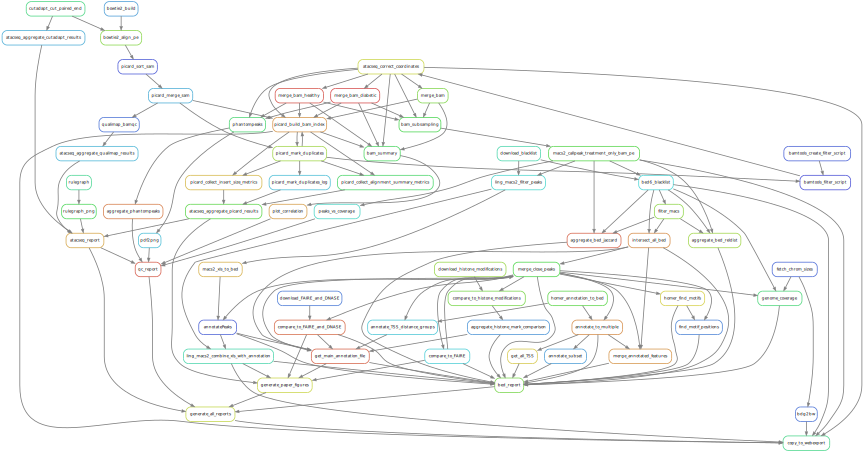
\includegraphics[height=.7\paperheight]{example_dags/rulegraph_complex.png}\hfil}\vfil}
	}
	\frame{
		\frametitle{Selecting Workflows}
		\begin{mdframed}[tikzsetting={draw=white,fill=white,fill opacity=0.8,
				line width=0pt},backgroundcolor=none,leftmargin=0,
			rightmargin=150,innertopmargin=4pt,roundcorner=10pt]
			\tableofcontents[currentsection,sections={1-4},hideothersubsections]
		\end{mdframed}
	}
}


%%%%%%%%%%%%%%%%%%%%%%%%%%%%%%%%%%%%%%%%%%%%%%%%%%%%%%%%%%%%%%%%%%%%%%%%%%%%%%%%
\begin{frame}
  \frametitle{What is this about?}
   \begin{question}[Questions]
   	 \begin{itemize}
       \item How do I get a workflow for a given scientific problem?
       \item How do I run such an arbitrary workflow?
     \end{itemize}
   \end{question} 
   \begin{docs}[Objectives]
   	  \begin{enumerate}
                      \item Introducing the workflow catalogue!
                      \item Learning the difference between ``curation'' (what some people think) and ``curation'' (what really works).
      \end{enumerate}
    \end{docs}
\end{frame}  

\subsection{The Snakemake Workflow Catalogue}

%%%%%%%%%%%%%%%%%%%%%%%%%%%%%%%%%%%%%%%%%%%%%%%%%%%%%%%%%%%%%%%%%%%%%%%%%%%%%%%
\begin{frame}
 \frametitle{Selecting and Downloading from the Workflow Catalogue}
 You can find the \Snakemake{} worfkflow catalogue, \lhref{https://snakemake.github.io/snakemake-workflow-catalog/?rules=true}{here}. It makes a difference between workflows which meet best-practice criteria - and those which do not.\newline
 \begin{columns}
   \begin{column}{0.5\textwidth}
     You can download and run any workflow. \Snakemake's portability features ensure it will work everywhere $\ldots$\pause
     \begin{warning}
     	$\ldots$ except, you most likely cannot, because of a missing cluster configuration.
     \end{warning}
   \end{column}
   \begin{column}{0.5\textwidth}
     \includegraphics[width=\textwidth]{Snakemake/Snakemake_Workflow_Catalog.png}
   \end{column}
 \end{columns}
\end{frame}

%%%%%%%%%%%%%%%%%%%%%%%%%%%%%%%%%%%%%%%%%%%%%%%%%%%%%%%%%%%%%%%%%%%%%%%%%%%%%%%
\begin{frame}
  \frametitle{Searching \emph{your} Workflow}
   \begin{columns}
  	\begin{column}{0.5\textwidth}
  		\includegraphics[width=\textwidth]{Snakemake/Searching_Workflows_in_Catalog.png}
  	\end{column}
  	\begin{column}{0.5\textwidth}
  		You can look for 
  		\begin{itemize}
  		  \item topical keywords and
  		  \item software
  		\end{itemize}
  	\end{column}
  \end{columns}
\end{frame}

%%%%%%%%%%%%%%%%%%%%%%%%%%%%%%%%%%%%%%%%%%%%%%%%%%%%%%%%%%%%%%%%%%%%%%%%%%%%%%%
\begin{frame}
	\frametitle{Workflows Compliance}
	\begin{question}[Noted this?]
	  \includegraphics[width=0.8\textwidth]{Snakemake/Snakemake_Workflow_Catalog_Categories.png}
	\end{question}
\end{frame}

%%%%%%%%%%%%%%%%%%%%%%%%%%%%%%%%%%%%%%%%%%%%%%%%%%%%%%%%%%%%%%%%%%%%%%%%%%%%%%%%
\begin{frame}[fragile]
  \frametitle{Deployment}
  Select (=click on) any desired workflow. There are three alternatives:
  \begin{enumerate}[<+->]
   \item a workflow offers a release - in which case you can download and unpack it
   \item all workflows offers a ``\altverb{git clone}'' hint
   \item or you use the \altverb{snakedeploy} to get everything you need.
  \end{enumerate}
\end{frame}

%%%%%%%%%%%%%%%%%%%%%%%%%%%%%%%%%%%%%%%%%%%%%%%%%%%%%%%%%%%%%%%%%%%%%%%%%%%%%%%%
\begin{frame}[fragile]
	\frametitle{Deployment II - Creating an Environment Fork}
	Usually, we can create an environment like:
	\begin{lstlisting}[language=Bash, style=Shell]
$ mamba create -c conda-forge -c bioconda -n snakemake \
> snakemake snakemake-executor-plugin-slurm \
> snakemake-storage-plugin-fs
    \end{lstlisting}
    This should install a \Snakemake{} environment with all necessary tools!
\end{frame}

%%%%%%%%%%%%%%%%%%%%%%%%%%%%%%%%%%%%%%%%%%%%%%%%%%%%%%%%%%%%%%%%%%%%%%%%%%%%%%%%
\begin{frame}[fragile]
	\frametitle{Deployment III - First Step!}
	Follow step 2 of a selected workflow usage instructions:
	\begin{columns}
		\begin{column}{0.4\textwidth}
			\centering
			\includegraphics[width=0.95\textwidth]{Snakemake/deploy_workflow}
		\end{column}
	    \begin{column}{0.6\textwidth}
	    	A usual command is:
	    	\begin{lstlisting}[language=Bash, style=Shell]
$ snakedeploy deploy-workflow \
> <URL>
	    	\end{lstlisting}
    	    This will create the directories \altverb{workflow} and \altverb{config} in your current directory.
    	    \begin{hint}
    	    	Alternatively, you may navigate to the repository of your desired workflow and download the entire workflow.
    	    \end{hint}
	    \end{column}
	\end{columns}
\end{frame}

%%%%%%%%%%%%%%%%%%%%%%%%%%%%%%%%%%%%%%%%%%%%%%%%%%%%%%%%%%%%%%%%%%%%%%%%%%%%%%%%
\begin{frame}[fragile]
	\frametitle{Finalizing the Deploymment}

		We could now deploy our sample workflow:
		\begin{itemize}
			\item Please create a directory \altverb{mkdir -p ~/example_workflow}
			\item Change to this directory.
			\item Deploy our sample workflow with
		\end{itemize}
        \begin{lstlisting}[language=Bash, style=Shell]
$ snakedeploy deploy-workflow \
> <++course.deploy_url++>
       \end{lstlisting}
\end{frame}


%%%%%%%%%%%%%%%%%%%%%%%%%%%%%%%%%%%%%%%%%%%%%%%%%%%%%%%%%%%%%%%%%%%%%%%%%%%%%%%%
\begin{frame}[fragile]
  \frametitle{Running Workflows on Cluster (or other environment)}
  Most likely a specific workflow never has been testing on \emph{your} computer before. It is almost ensured it will run on arbitrary servers, but clusters are a different story. \newline
  So
  \begin{itemize}[<+->]
   \item try to parameterize your workflow as we will learn and create a "profile"
   \item if it gives issues and you know how to correct it, ``fork'' the worklow and create a pull request
   \item if you cannot fix it, create a bug report
  \end{itemize}
\end{frame}

%%%%%%%%%%%%%%%%%%%%%%%%%%%%%%%%%%%%%%%%%%%%%%%%%%%%%%%%%%%%%%%%%%%%%%%%%%%%%%%%
\begin{frame}
  \frametitle{\Interlude{Learn git!}}
  If you do not know what ``fork'' and ``pull request'' means, learn git!
  \begin{itemize}[<+->]
   \item there are courses
   \item and lots of online material
   \item and books
  \end{itemize}
  \pause
  \begin{warning}
  	Knowing git is essential in data analysis!
  \end{warning}
\end{frame}

%%%%%%%%%%%%%%%%%%%%%%%%%%%%%%%%%%%%%%%%%%%%%%%%%%%%%%%%%%%%%%%%%%%%%%%%%%%%%%%%
\begin{frame}[fragile]
  \frametitle{\HandsOn{Configuring the Workflow}}
  It is now time to configure and parameterize the workflow.
  \pause
  \begin{hint}
  	As the configuration is workflow dependent you need to follow instructions, now.
  \end{hint}
  \pause
  Eventually start the workflow using:
  \begin{lstlisting}[language=Bash, style=Shell]
$ snakemake --executor slurm \
> -j unlimited \
> --configfile <path to file> \
> --workflow-profile <path to directory> \
> --directory <path to your course output>
  \end{lstlisting}
  \pause
  \begin{hint}
  	We will learn a few tricks to shorten this line.
  \end{hint}
\end{frame}



%%%%%%%%%%%%%%%%%%%%%%%%%%%%%%%%%%%%%%%%%%%%%%%%%%%%%%%%%%%%%%%%%%%%%%%%%%%%%%%%
% \include{common/Using_Workflow_Configs}

%%%%%%%%%%%%%%%%%%%%%%%%%%%%%%%%%%%%%%%%%%%%%%%%%%%%%%%%%%%%%%%%%%%%%%%%%%%%%%%%
%%%%%%%%%%%%%%%%%%%%%%%%%%%%%%%%%%%%%%%%%%%%%%%%%%%%%%%%%%%%%%%%%%%%%%%%%%%%%%%%
\section{Plotting DAGs}
{   
	\usebackgroundtemplate{
		\vbox to \paperheight{\vfil\hbox to \paperwidth{\hfil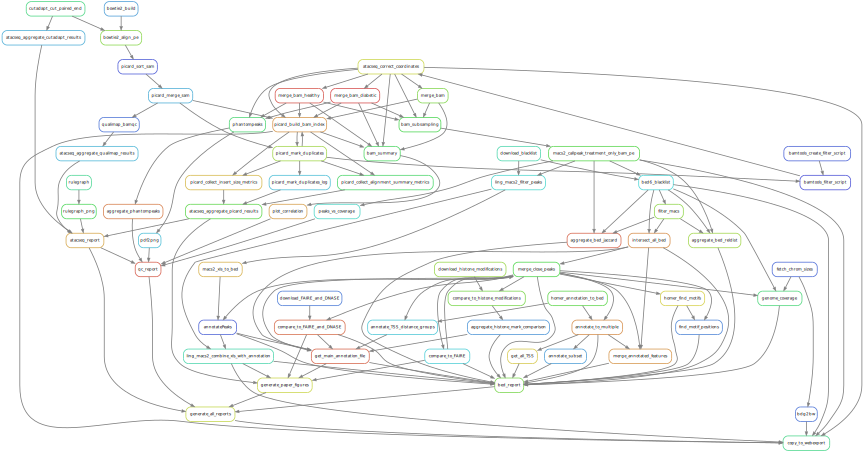
\includegraphics[height=\paperheight]{example_dags/rulegraph_complex.png}\hfil}\vfil}
		% source: https://en.m.wikipedia.org/wiki/File:Text-x-python.svg
	}
	\frame{
		\frametitle{Plotting Workflow Graphs}
		\begin{mdframed}[tikzsetting={draw=white,fill=white,fill opacity=0.8,
				line width=0pt},backgroundcolor=none,leftmargin=0,
			rightmargin=150,innertopmargin=4pt,roundcorner=10pt]
			\tableofcontents[currentsection,sections={1-4},hideothersubsections]
		\end{mdframed}
	}
}

%%%%%%%%%%%%%%%%%%%%%%%%%%%%%%%%%%%%%%%%%%%%%%%%%%%%%%%%%%%%%%%%%%%%%%%%%%%%%%%%
\begin{frame}
  \frametitle{What is this about?}
   \begin{question}[Questions]
   	 \begin{itemize}
       \item How do we plot our workflows for a publication?
     \end{itemize}
   \end{question}
   \begin{docs}[Objectives]
   	  \begin{enumerate} 
                      \item Learn to plot workflows using \Snakemake{} and GraphViz.
      \end{enumerate}
   \end{docs}
\end{frame}

%%%%%%%%%%%%%%%%%%%%%%%%%%%%%%%%%%%%%%%%%%%%%%%%%%%%%%%%%%%%%%%%%%%%%%%%%%%%%%%%
\begin{frame}[fragile]
  \frametitle{\HandsOn{Plotting the Workflow}}
  \Snakemake{} has a build-in plotting feature. Run 
  \begin{lstlisting}[language=Bash, style=Shell]
$ snakemake --rulegraph | dot -Tpng > <your_workflow.png>
  \end{lstlisting}
  to plot your workflow graph. And
  \begin{lstlisting}[language=Bash, style=Shell]
$ display <your_workflow.png>
  \end{lstlisting}
  to display the workflow.
\end{frame}

%%%%%%%%%%%%%%%%%%%%%%%%%%%%%%%%%%%%%%%%%%%%%%%%%%%%%%%%%%%%%%%%%%%%%%%%%%%%%%%%
\begin{frame}
  \frametitle{Your DAG:}
  \centering
  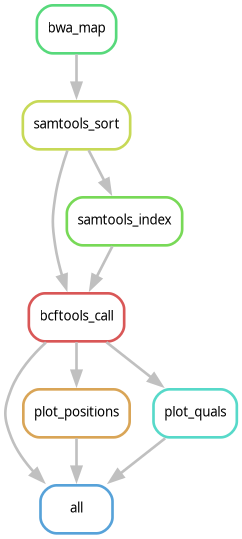
\includegraphics[height=0.5\textheight]{workflows/rulegraph_lifescience.png}
\end{frame}

%%%%%%%%%%%%%%%%%%%%%%%%%%%%%%%%%%%%%%%%%%%%%%%%%%%%%%%%%%%%%%%%%%%%%%%%%%%%%%%%
\begin{frame}[fragile]
  \frametitle{\HandsOn{Produce different Plots}}
  What do you observe, if you try:
  \begin{lstlisting}[language=Bash, style=Shell,basicstyle=\footnotesize]
$ snakemake --rulegraph | dot -Tpng > <your_rulegraph.png>
$ # or
$ snakemake --filegraph | dot -Tpng > <your_filegraph.png>
$ # or
$ snakemake --dag | dot -Tpng > <your_dag.png>
$ # or --dag again after
$ snakemake --delete-all-output -c1
  \end{lstlisting}
\end{frame}

%%%%%%%%%%%%%%%%%%%%%%%%%%%%%%%%%%%%%%%%%%%%%%%%%%%%%%%%%%%%%%%%%%%%%%%%%%%%%%%%
\begin{frame}[fragile]
 \frametitle{Plot Comparison}
 \begin{figure}
  \centering
  \subfloat[\centering \altverb{--rulegraph}]{{ 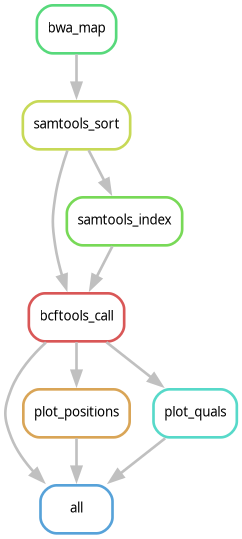
\includegraphics[width=0.2\textwidth, height=0.5\textheight]{workflows/rulegraph_lifescience.png} }}
  \subfloat[\centering \altverb{--filegraph}]{{ 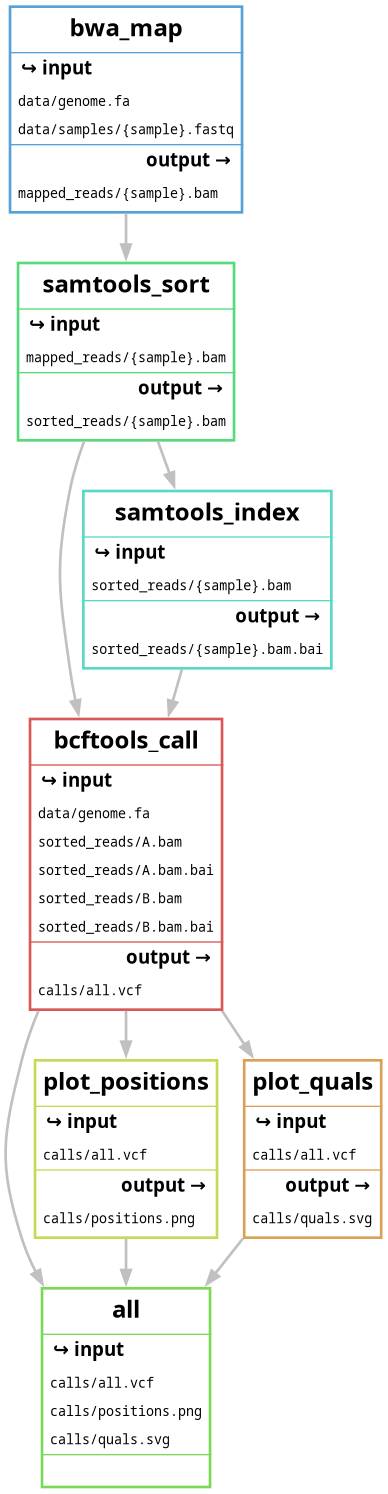
\includegraphics[width=0.2\textwidth, height=0.5\textheight]{workflows/filegraph_lifescience.png} }}
  \subfloat[\centering \altverb{--dag}, with rules done]{{ 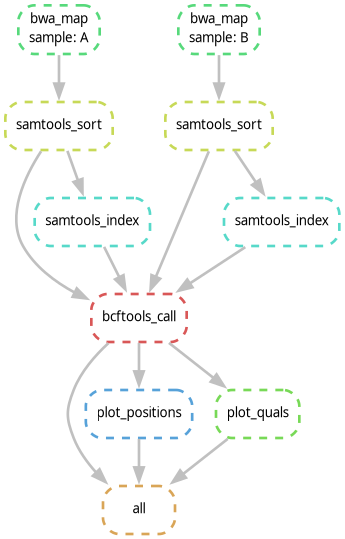
\includegraphics[width=0.2\textwidth, height=0.5\textheight]{workflows/dag_lifescience.png} }}
  \subfloat[\centering \altverb{--dag}, with rules still to do]{{ 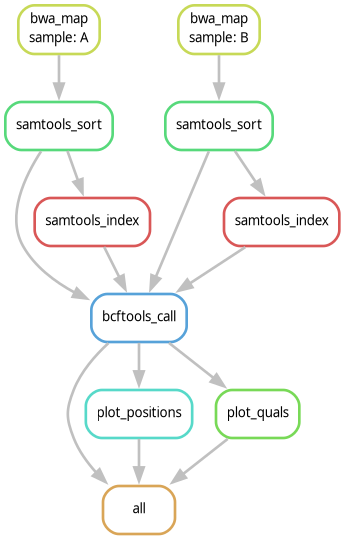
\includegraphics[width=0.2\textwidth, height=0.5\textheight]{workflows/dag_full_lifescience.png} }}
\end{figure}

\end{frame}






%%%%%%%%%%%%%%%%%%%%%%%%%%%%%%%%%%%%%%%%%%%%%%%%%%%%%%%%%%%%%%%%%%%%%%%%%%%%%%%%
%%%%%%%%%%%%%%%%%%%%%%%%%%%%%%%%%%%%%%%%%%%%%%%%%%%%%%%%%%%%%%%%%%%%%%%%%%%%%%%%
\section{How does Clustercomputing work?}
{   
	\usebackgroundtemplate{
		\vbox to \paperheight{\vfil\hbox to \paperwidth{\hfil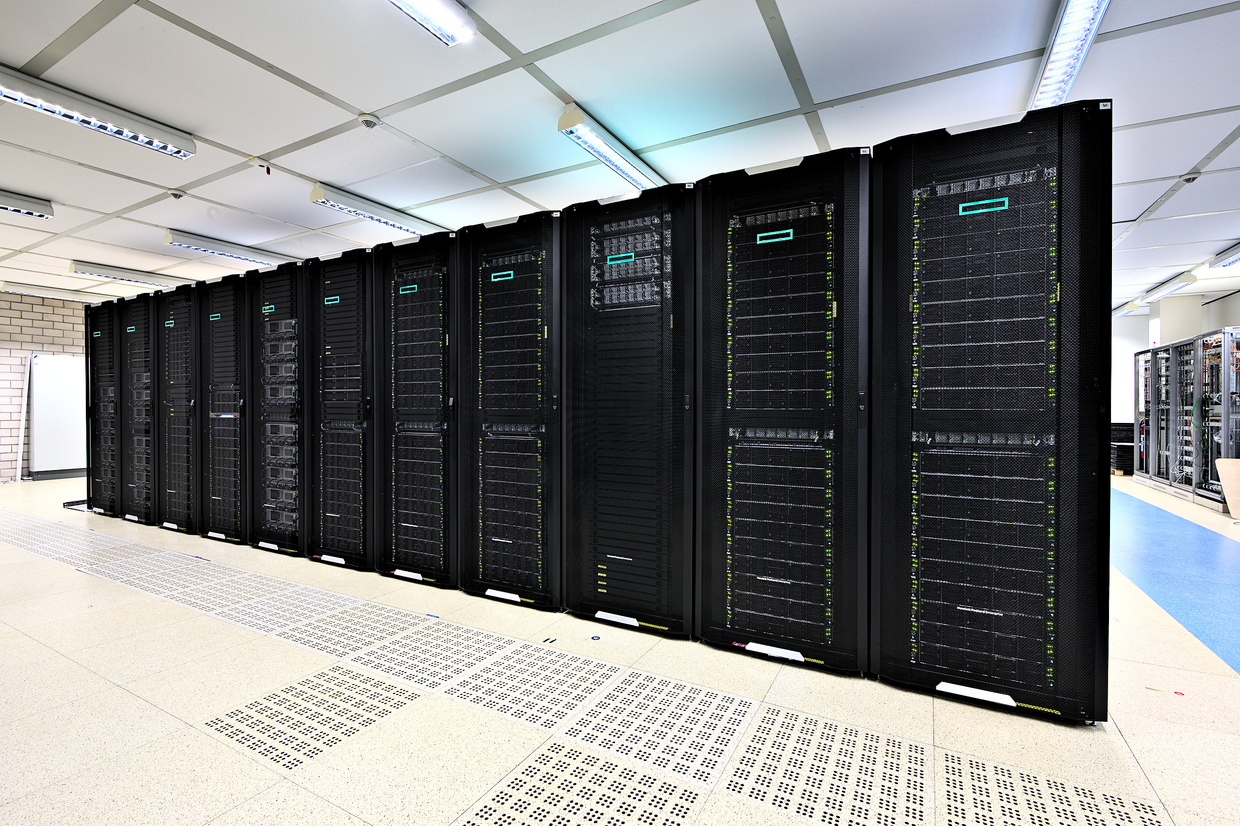
\includegraphics[height=\paperheight]{misc/cluster_kit}\hfil}\vfil}
		% source: https://en.m.wikipedia.org/wiki/File:Text-x-python.svg
	}
	\frame{
		\frametitle{Running ordinary Batch Scripts}
		\begin{mdframed}[tikzsetting={draw=white,fill=white,fill opacity=0.8,
				line width=0pt},backgroundcolor=none,leftmargin=0,
			rightmargin=150,innertopmargin=4pt,roundcorner=10pt]
			\tableofcontents[currentsection,sections={1-4},hideothersubsections]
		\end{mdframed}
	}
}


%%%%%%%%%%%%%%%%%%%%%%%%%%%%%%%%%%%%%%%%%%%%%%%%%%%%%%%%%%%%%%%%%%%%%%%%%%%%%%%%
\begin{frame}
  \frametitle{What is this about?}
    \begin{question}
   	  \begin{itemize}
        \item How does ordinary job submission work on a cluster?
        \item How does it work using Snakemake? (Which parameterization is necessary?)
      \end{itemize}
   \end{question}
   \begin{docs}[Objectives]
   	 \begin{enumerate}
   	 	\item Get a feeling for the SLURM batch system.
   	 	\item We want to give you an idea of building a workflow with \emph{pure} batch system commands, first.
     \end{enumerate}
   \end{docs}
\end{frame}


%%%%%%%%%%%%%%%%%%%%%%%%%%%%%%%%%%%%%%%%%%%%%%%%%%%%%%%%%%%%%%%%%%%%%%%%%%%%%%%%
\subsection*{The \slurm Scheduler}

%%%%%%%%%%%%%%%%%%%%%%%%%%%%%%%%%%%%%%%%%%%%%%%%%%%%%%%%%%%%%%%%%%%%%%%%%%%%%%%% 
\begin{frame}
  \frametitle{What is a scheduler?}
  On HPC systems you do not \emph{just start}, you need a \emph{``scheduler''}.
  So, what's that?\newline
  A scheduler (or ``batch system'') on a HPC system should\ldots
  \begin{itemize}
  \item provide an interface to help defining workflows and/or job dependencies
  \item enable automatic submission of executions
  \item provide interfaces to monitor the executions
  \item prioritise the execution order of unrelated jobs
  \end{itemize}
  \begin{columns}
    \begin{column}{0.8\linewidth}
      This is an micro-intro to the \slurm batch system.
    \end{column}
    \begin{column}{0.2\linewidth}
      \begin{figure}
        \centering
        \includegraphics[height=1.5cm,width=1.5cm]{logos/slurm_logo.png}
      \end{figure}
    \end{column}
  \end{columns}
  \vfill
\end{frame}

%%%%%%%%%%%%%%%%%%%%%%%%%%%%%%%%%%%%%%%%%%%%%%%%%%%%%%%%%%%%%%%%%%%%%%%%%%%%%%%% 
\begin{frame}
  \frametitle{Promises, promises and even more promises}
  How does a scheduler work?
  \pause
  \begin{block}{You tell it\ldots}
    \begin{itemize}
    \item how much memory (RAM, scratch space) your job will need.\pause
    \item how much time you will spend on it.\pause
    \item how many CPUs you will need (and in which combination).\pause
    \item whether you need something special (e.g. a GPU).
    \end{itemize}
  \end{block}
  \pause \vspace{-0.2cm}
  \begin{exampleblock}{The scheduler will act:}
    \begin{itemize}
    \item It will queue up your job (and decide when it will start relative to others).\pause
    \item It will decide where your job will run physically (which hosts).\pause
    \item Eventually it will start your job (if everything was correct).
    \end{itemize}
  \end{exampleblock}
  \vfill
\end{frame}

\setcounter{preframe_handson}{\value{handson}}
%%%%%%%%%%%%%%%%%%%%%%%%%%%%%%%%%%%%%%%%%%%%%%%%%%%%%%%%%%%%%%%%%%%%%%%%%%%%%%%% 
\begin{frame}[fragile]
  \setcounter{handson}{\value{preframe_handson}}
  \frametitle{\HandsOn{Your first job script}}
  \begin{hint}
  	    From now on, we will be scripting examples (cloze-based). For this you will
        need an editor. If you do not know any other editor, use \texttt{gedit}:
  \end{hint}
  \begin{lstlisting}[language=Bash, style=Shell, basicstyle=\scriptsize]
$ # cd into appropriate directory
$ # Start gedit with the command 
$ gedit &
  \end{lstlisting}
  \begin{hint}
  	The \texttt{\&} will put the editor into the background.
  \end{hint} 
\end{frame}

%%%%%%%%%%%%%%%%%%%%%%%%%%%%%%%%%%%%%%%%%%%%%%%%%%%%%%%%%%%%%%%%%%%%%%%%%%%%%%% 
\input{<++course.hello_world_script++>}

%%%%%%%%%%%%%%%%%%%%%%%%%%%%%%%%%%%%%%%%%%%%%%%%%%%%%%%%%%%%%%%%%%%%%%%%%%%%%%%% 
\begin{frame}[fragile]%
	\frametitle{Please Imaging \ldots}
	Now, thing of your analysis workflow: QC, preprocessing, processing, analysis, post-processing and plotting and \ldots \newline
	\pause
	All this \emph{can} be achieved with SLURM, too all with bash:
	\begin{lstlisting}[language=Bash, style=Shell]
# First, do some pre-processing for the first job.
...
# Then, submit a job without dependencies.
jid1=$(sbatch ... job1.sh)
# NOTE: ALL 'job*sh' scripts are bash scripts,
#       with more logic than the "hello world" script.		

# Next, do some more logic as pre-processing for the 
# follow-up jobs. ...
# multiple jobs can depend on a single job
jid2=$(sbatch --dependency=afterany:$jid1 ... job2.sh)
jid3=$(sbatch --dependency=afterany:$jid1 ... job3.sh)
	\end{lstlisting}
    etc. can easily be a few thousand lines for \emph{every} workflow.
	\vfill
\end{frame}


%%%%%%%%%%%%%%%%%%%%%%%%%%%%%%%%%%%%%%%%%%%%%%%%%%%%%%%%%%%%%%%%%%%%%%%%%%%%%%%% 
\begin{frame}
  \frametitle{End of HPC Intro}
  We could co on with \emph{many} details with regards to the scheduler, the file system, etc..
  \begin{block}{HPC Courses}
   HPC teams offers courses to:
   \begin{itemize}
    \item HPC Intro
    \item Bash Intro
    \item Research Data Management
    \item many other topics
   \end{itemize}
  \end{block}
  \pause
  \begin{hint}[What's next]
      We are going to parameterize our workflow\textbf{s} for clusters and for our applications in \Snakemake!
  \end{hint}
\end{frame}







%%%%%%%%%%%%%%%%%%%%%%%%%%%%%%%%%%%%%%%%%%%%%%%%%%%%%%%%%%%%%%%%%%%%%%%%%%%%%%%%
%%%%%%%%%%%%%%%%%%%%%%%%%%%%%%%%%%%%%%%%%%%%%%%%%%%%%%%%%%%%%%%%%%%%%%%%%%%%%%%%
\section{Parameterizing your Workflow (II) - I/O}
{   
	\usebackgroundtemplate{
		\vbox to \paperheight{\vfil\hbox to \paperwidth{\hfil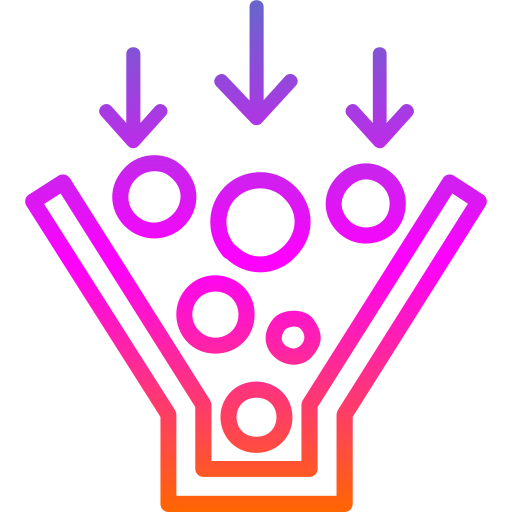
\includegraphics[height=\paperheight]{misc/bottleneck.png}\hfil}\vfil}
	}
	\frame{
		\frametitle{Avoiding I/O Contention}
		\begin{mdframed}[tikzsetting={draw=white,fill=white,fill opacity=0.8,
				line width=0pt},backgroundcolor=none,leftmargin=0,
			rightmargin=150,innertopmargin=4pt,roundcorner=10pt]
			\tableofcontents[currentsection,sections={1-4},hideothersubsections]
			\vspace{1em}
			\tiny \lhref{https://www.flaticon.com/free-icon/bottleneck_10803803}{from Flaticon}
		\end{mdframed}
	}
}
%%%%%%%%%%%%%%%%%%%%%%%%%%%%%%%%%%%%%%%%%%%%%%%%%%%%%%%%%%%%%%%%%%%%%%%%%%%%%%%%
\begin{frame}
  \frametitle{What is this about?}
  \begin{question}[Questions]
   	\begin{itemize}
      \item How do we avoid I/O contention?
      \item How do we account for file system latency?
    \end{itemize}
  \end{question}
   \begin{docs}[Objectives]
   	 \begin{enumerate} 
        \item Learn how to tune \Snakemake{} to mitigate I/O contention.
        \item Learn how to configure \Snakemake{} to allow for file system latency.
    \end{enumerate}
  \end{docs}
\end{frame}

%%%%%%%%%%%%%%%%%%%%%%%%%%%%%%%%%%%%%%%%%%%%%%%%%%%%%%%%%%%%%%%%%%%%%%%%%%%%%%%%
\begin{frame}
	\frametitle{\Interlude{What is Random Access?}}
	\vspace{-1.5em}
	\begin{figure}
		\centering
		\begin{tikzpicture}
			\node[name=sa] at (3.5,10) { \lhref{https://en.wikipedia.org/wiki/Random_access}{Sequential Access} };
			\foreach[count=\y from 2] \x in {1,...,11}{
				\draw[thick,black,midway,draw] (\x,8.75) rectangle node[name=s\x] {} (\y,8.25);
			}       
			\foreach[count=\y from 2] \x in  {1, ..., 10} {
					\path[->] ([yshift=.6em]s\x.north west) edge[bend left=30] ([yshift=.6em]s\y.north west);
			}
			%         \path[->] ([yshift=.6em]s1.north) edge [bend left=30] ([yshift=.6em]s2.north) ;
			
			\node[name=ra] at (3.5,7) { Random Access };
			\foreach[count=\y from 2] \x in {1,...,11}{
				\draw[thick,black,midway,draw] (\x,5.75) rectangle node[name=r\x] {} (\y,5.25);
			}
		
			\path[->] ([yshift=.6em]r1.north) edge [bend left=30] ([yshift=.6em]r5.north) ;
			\path[->] ([yshift=.6em]r5.north) edge [bend right=60] ([yshift=.6em]r2.north) ;
			\path[->] ([yshift=.6em]r2.north) edge [bend left=30] ([yshift=.6em]r3.north) ;
			\path[->] ([yshift=.6em]r3.north) edge [bend left=30] ([yshift=.6em]r11.north) ;
			\path[->] ([yshift=.6em]r11.north) edge [bend right=30] ([yshift=.6em]r7.north) ;
			\path[->] ([yshift=.6em]r7.north) edge [bend right=30] ([yshift=.6em]r6.north) ;
			\path[->] ([yshift=.6em]r6.north) edge [bend left=60] ([yshift=.6em]r8.north) ;
			\path[->] ([yshift=.6em]r8.north) edge [bend right=50] ([yshift=.6em]r4.north) ;
		\end{tikzpicture}
	\end{figure}
\end{frame}

%%%%%%%%%%%%%%%%%%%%%%%%%%%%%%%%%%%%%%%%%%%%%%%%%%%%%%%%%%%%%%%%%%%%%%%%%%%%%%%%
\begin{frame}
	\frametitle{\Interlude{What is Random Access?}}
	\begin{question}
	  \begin{itemize}
	  	\item What causes Random Access?
	  	\item Why is it harmful? What can we do?
	  \end{itemize}
    \end{question}
	\pause
	\begin{columns}[t]
	  \begin{column}{0.5\textwidth}
	  	Causes:
	  	\hrule
	  	\begin{itemize}
	  	  \item a number of (threaded) apps accessing the same file space (e.g. reference data)
	  	  \item a number of apps accessing a file space exceeding the file system cache size
	  	\end{itemize}
  	     Will slow parallel file systems and your data analysis!
	  \end{column}
      \begin{column}{0.5\textwidth}
      	Remedies:
      	\hrule
      	\begin{itemize}
      		\item copy data to/from compute nodes equipped with SSD
      		\item use a RAM disk (RAM = random access memory) - which many clusters provide
      	\end{itemize}
      \end{column}
	\end{columns}	
\end{frame}

%%%%%%%%%%%%%%%%%%%%%%%%%%%%%%%%%%%%%%%%%%%%%%%%%%%%%%%%%%%%%%%%%%%%%%%%%%%%%%%%
\begin{frame}
  \frametitle{\Interlude{What is File System Latency?}}
    \centering
	\begin{tikzpicture}[line cap=rect,line width=3pt, 
		datastore/.style={draw, rounded rectangle, rounded rectangle east arc=concave, rounded rectangle arc length=150},
		]
	  \tikzstyle{storage} = [rectangle, minimum width=3cm, minimum height=1cm, text width=3cm, text centered, draw=black]
	  
	  \filldraw [fill=cyan] (0,0) circle [radius=1cm];
	  \foreach \angle [count=\xi] in {60,30,...,-270}
	  {
		\draw[line width=0.5pt] (\angle:0.9cm) -- (\angle:1cm);
		\node[font=\small] at (\angle:0.68cm) {\textsf{\xi}};
	  }
	  \foreach \angle in {0,90,180,270}
	  \draw[line width=1pt] (\angle:0.8cm) -- (\angle:1cm);
	  \draw (0,0) -- (120:0.4cm);
	  \draw (0,0) -- (90:.5cm);
	  
	  \node (sto1) [datastore] at (-4, 0) {Storage};
	  \node at (4, 0) {\includegraphics[width=.25\textwidth]{misc/data_center.png}};
  \end{tikzpicture}
  \begin{docs}{File System Latency}
  	The time it takes from the file system to the client and back.
  \end{docs}
\end{frame}

%%%%%%%%%%%%%%%%%%%%%%%%%%%%%%%%%%%%%%%%%%%%%%%%%%%%%%%%%%%%%%%%%%%%%%%%%%%%%%%%
\begin{frame}
  \frametitle{\Interlude{What is File System Latency? II}}
  \begin{docs}{Background}
  	Some clusters use NFS (Network File System). There, file system latency \emph{can} be an issue.\newline
  	\pause
  	On parallel file systems, the latency usually is very low. 
  \end{docs}	
\end{frame}


%%%%%%%%%%%%%%%%%%%%%%%%%%%%%%%%%%%%%%%%%%%%%%%%%%%%%%%%%%%%%%%%%%%%%%%%%%%%%%%%
\subsection{Global Workflow Configuration}

%%%%%%%%%%%%%%%%%%%%%%%%%%%%%%%%%%%%%%%%%%%%%%%%%%%%%%%%%%%%%%%%%%%%%%%%%%%%%%%%
\begin{frame}[fragile]
  \frametitle{\Snakemake{} Profiles}
  \begin{hint}
  	Profiles can shorten your command lines and be an easy remedy for the described issues!
  \end{hint}
  \pause
  Two kinds of profiles are supported:
  \begin{itemize}[<+->]
  	\item A global profile that is defined in a system-wide or user-specific configuration directory (on Linux, this will be \altverb{\~/.config/snakemake} and \altverb{/etc/xdg/snakemake}, you can find the answer for your system via \altverb{snakemake --help}).
  	\item A workflow specific profile that is defined via a flag (\altverb{--workflow-profile}) or searched in a default location (profile/default) in the working directory or next to the \altverb{Snakefile}.
  \end{itemize}
\end{frame}

%%%%%%%%%%%%%%%%%%%%%%%%%%%%%%%%%%%%%%%%%%%%%%%%%%%%%%%%%%%%%%%%%%%%%%%%%%%%%%%%
\begin{frame}[fragile]
  \frametitle{Your Profile}
    \begin{onlyenv}<1| handout:0>
      Your first line forces the executor to be set to \slurm - persistently.
      \begin{lstlisting}[language=Bash, style=Shell]
executor: slurm
     \end{lstlisting}
     No more, \altverb{snakemake --executor slurm ...}!
   \end{onlyenv}
   \begin{onlyenv}<2| handout:0>
   	 The next line tells \Snakemake to wait for 5 seconds, if output files are not present (because we are working with parallel file systems). 
   	 \begin{lstlisting}[language=Bash, style=Shell]
executor: slurm
latency-wait: 5
   	 \end{lstlisting}
    \end{onlyenv}
    \begin{onlyenv}<3| handout:0>
      The entire rest, will tell the storage plugin (\altverb{snakemake-storage-plugin-fs}) to stage in to the node-local storage on your cluster, for \emph{every} job and to copy back your results. When dealing with I/O intensive jobs, this can boost your performance tremendously. 
      \begin{lstlisting}[language=Bash, style=Shell]
executor: slurm
latency-wait: 5
default-storage-provider: fs
shared-fs-usage:
  - persistence
  - sources
  - source-cache
remote-job-local-storage-prefix: |
    <++cluster.remotejoblocalstorageprefix++>
local-storage-prefix: <++cluster.localstorageprefix++>
    \end{lstlisting}
   \end{onlyenv}
   \begin{onlyenv}<4| handout:1>
   	The complete configuration out to be in \altverb{\~/.config/snakemake/config.yaml}
   	\begin{lstlisting}[language=Bash, style=Shell]
executor: slurm
latency-wait: 5
default-storage-provider: fs
shared-fs-usage:
  - persistence
  - sources
  - source-cache
remote-job-local-storage-prefix: |
     <++cluster.remotejoblocalstorageprefix++>
local-storage-prefix: <++cluster.localstorageprefix++>
    \end{lstlisting}
  \end{onlyenv}
\end{frame}


%%%%%%%%%%%%%%%%%%%%%%%%%%%%%%%%%%%%%%%%%%%%%%%%%%%%%%%%%%%%%%%%%%%%%%%%%%%%%%%%
\begin{frame}[fragile]
	\frametitle{\HandsOn{Running with a Profile I}}
	Enter 
	\begin{lstlisting}[language=Bash, style=Shell]
export SNAKEMAKE_PROFILE="$HOME/.config/snakemake"
    \end{lstlisting}
	in your \altverb{.bashrc}
\end{frame}

%%%%%%%%%%%%%%%%%%%%%%%%%%%%%%%%%%%%%%%%%%%%%%%%%%%%%%%%%%%%%%%%%%%%%%%%%%%%%%%%
\begin{frame}[fragile]
	\frametitle{\HandsOn{Running with a Profile II}}
	Copy the configuration file:
	\begin{lstlisting}[language=Bash, style=Shell]
$ mkdir -p ~/.config/snakemake
$ cp ~/workflows/config.yaml \
> ~/.config/snakemake/.
	\end{lstlisting}
    Activate the new settings:
    \begin{lstlisting}[language=Bash, style=Shell]
$ source ~/.bashrc
    \end{lstlisting}
    And run the workflow - just for fun:
    \begin{lstlisting}[language=Bash, style=Shell]
$ snakemake -F # just this one flag!
    \end{lstlisting}
\end{frame}

	


      
%%%%%%%%%%%%%%%%%%%%%%%%%%%%%%%%%%%%%%%%%%%%%%%%%%%%%%%%%%%%%%%%%%%%%%%%%%%%%%%%
\include{common/Reports}    

%%%%%%%%%%%%%%%%%%%%%%%%%%%%%%%%%%%%%%%%%%%%%%%%%%%%%%%%%%%%%%%%%%%%%%%%%%%%%%%%
%%%%%%%%%%%%%%%%%%%%%%%%%%%%%%%%%%%%%%%%%%%%%%%%%%%%%%%%%%%%%%%%%%%%%%%%%%%%%%%%%
\section{Snakemake Wrappers}
{   
	\usebackgroundtemplate{
		\vbox to \paperheight{\vfil\hbox to \paperwidth{\hfil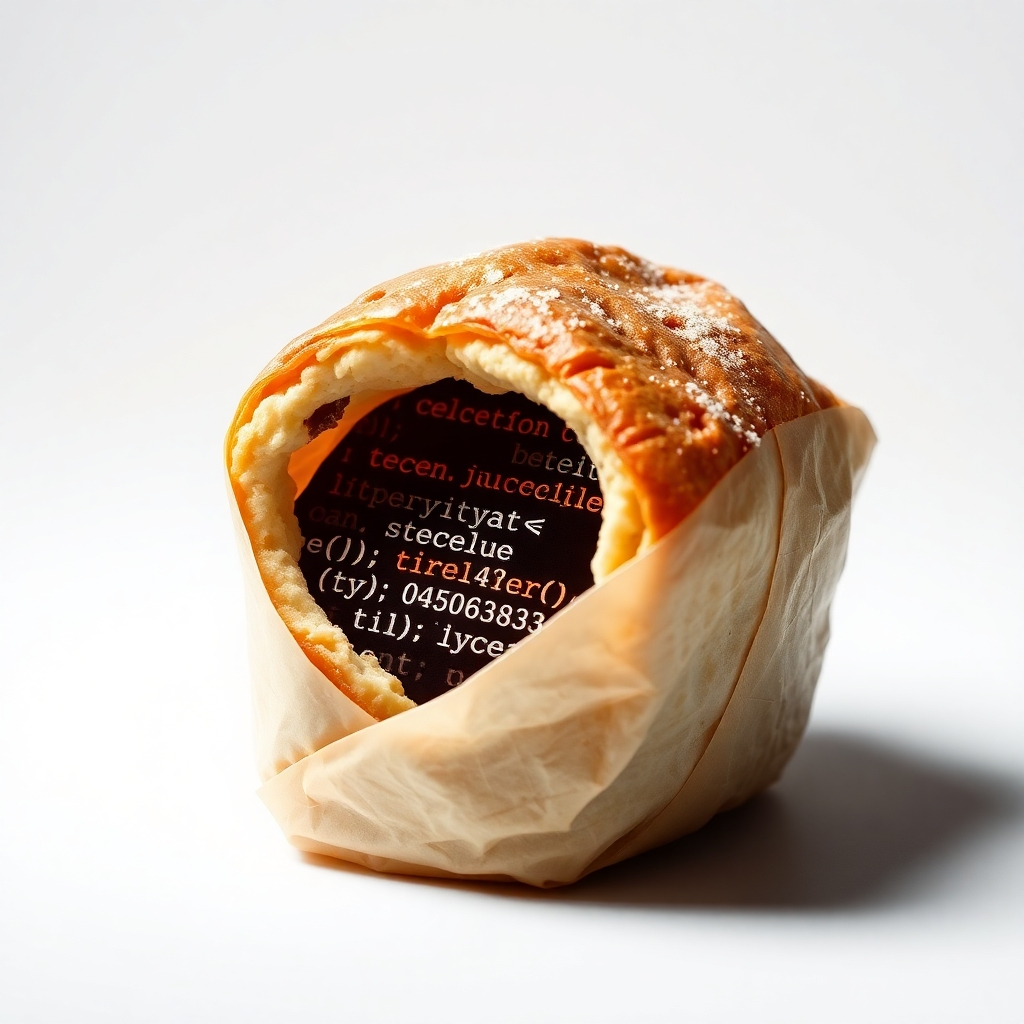
\includegraphics[height=.7\paperheight]{misc/wrapper.jpg}\hfil}\vfil}
	}
	\frame{
		\frametitle{Using \Snakemake-Wrappers}
		\begin{mdframed}[tikzsetting={draw=white,fill=white,fill opacity=0.8,
				line width=0pt},backgroundcolor=none,leftmargin=0,
			rightmargin=150,innertopmargin=4pt,roundcorner=10pt]
			\tableofcontents[currentsection,sections={1-4},hideothersubsections]
		\end{mdframed}
	}
}

%%%%%%%%%%%%%%%%%%%%%%%%%%%%%%%%%%%%%%%%%%%%%%%%%%%%%%%%%%%%%%%%%%%%%%%%%%%%%%%%
\subsection{Using Wrappers}

%%%%%%%%%%%%%%%%%%%%%%%%%%%%%%%%%%%%%%%%%%%%%%%%%%%%%%%%%%%%%%%%%%%%%%%%%%%%%%%%
\begin{frame}
    \frametitle{What is this about?}
    \begin{question}[Questions]
        \begin{itemize}
            \item What is a \Snakemake{} Wrapper?
            \item How can \Snakemake{} wrappers be used to write reproducible workflows?
        \end{itemize}
    \end{question}
    \begin{docs}[Objectives]
        \begin{enumerate}
            \item Introduce the concept of \Snakemake{} wrappers
            \item Include \Snakemake{} wrappers in your workflows
            \item Reproducibility of \Snakemake{} wrappers
        \end{enumerate}
    \end{docs}
\end{frame}

%%%%%%%%%%%%%%%%%%%%%%%%%%%%%%%%%%%%%%%%%%%%%%%%%%%%%%%%%%%%%%%%%%%%%%%%%%%%%%%%
\begin{frame}{Introduction to Wrappers}
    For a single tool, \Snakemake{} Wrappers do:
    \begin{itemize}[<+->]
        \item Document usage
        \item Describe the dependencies
        \item Provide a way to call the tool with information from Snakemake
    \end{itemize}
    This setup makes Snakemake wrappers reusable across multiple workflows.
\end{frame}

%%%%%%%%%%%%%%%%%%%%%%%%%%%%%%%%%%%%%%%%%%%%%%%%%%%%%%%%%%%%%%%%%%%%%%%%%%%%%%%%
\begin{frame}{Introduction to Wrappers}
    Wrappers consist of three components:
    \begin{enumerate}
        \item A description of their usage (\altverb{meta.yaml})
        \item A conda environment description of all dependencies of the tool (\altverb{environment.yaml})
        \item A python script that invokes the tool (\altverb{wrapper.py})
    \end{enumerate}
    Since they are reusable, there is a large repository online of tried and tested 
    wrappers written by the community:
    \pause
    \begin{docs}
    	You can browse the \lhref{https://snakemake-wrappers.readthedocs.io}{snakemake-wrapper overview page} to select your desired wrapper. New Wrappers are added frequently.
    \end{docs}
\end{frame}

%%%%%%%%%%%%%%%%%%%%%%%%%%%%%%%%%%%%%%%%%%%%%%%%%%%%%%%%%%%%%%%%%%%%%%%%%%%%%%%%
\begin{frame}[fragile]
	\frametitle{\Interlude{Dealing with multiple Extensions}}
	\begin{warning}
		So far, we were referring to \emph{one} file. But alignment software like \altverb{bwa} requires all those files with multiple extensions! {\bf This is not safe!}
	\end{warning}
    To require multiple extensions \Snakemake provides the \altverb{multiext()}-function:
    \begin{lstlisting}[language=Python,style=Python]
rule bwa_map:
    input:
      ...
      idx=multiext("genome", ".amb", ".fa",
                   ".ann", ".bwt", ".pac", ".sa")
      ...
    \end{lstlisting}
	Now, \emph{all} listed extensions are required to be present for the file with the prefix \altverb{genome}!
\end{frame}



%%%%%%%%%%%%%%%%%%%%%%%%%%%%%%%%%%%%%%%%%%%%%%%%%%%%%%%%%%%%%%%%%%%%%%%%%%%%%%%%
\begin{frame}[fragile]{Using Wrappers - The Example}
	\begin{docs}
		The following example uses the \altverb{bwa-mem} wrapper from the \Snakemake-community wrappers repository. The example is specific and let us illustrate the usage.
		We will cover the usage step by step and specifically:
		\begin{itemize}
			\item How to find a wrapper?
			\item How to use a wrapper.
		\end{itemize}
	\end{docs}
\end{frame}

%%%%%%%%%%%%%%%%%%%%%%%%%%%%%%%%%%%%%%%%%%%%%%%%%%%%%%%%%%%%%%%%%%%%%%%%%%%%%%%%
\begin{frame}[fragile]{Using Wrappers}
    Using \Snakemake{} wrappers ease your life as a workflow programmer:
    \begin{lstlisting}[language=Python,style=Python,basicstyle=\footnotesize]
rule bwa_map:
    input:
        reads=["input/{sample}_1.fq.gz", 
               "input/{sample}_2.fq.gz"],
        idx=multiext("genome", ".amb", 
                 ".ann", ".bwt", ".pac", ".sa"),
    output:
        "output/{sample}.bam"
    params:
        extra=r"-R '@RG\tID:{sample}\tSM:{sample}'",
        sorting="none",  
        sort_order="queryname",  
        sort_extra="", 
    threads: 8
    wrapper:
        "v3.2.0/bio/bwa/mem"
    \end{lstlisting}
\end{frame}

%%%%%%%%%%%%%%%%%%%%%%%%%%%%%%%%%%%%%%%%%%%%%%%%%%%%%%%%%%%%%%%%%%%%%%%%%%%%%%%%
\begin{frame}[fragile]{Using Wrappers: Calling a Wrapper}
	The \altverb{wrapper} directive signals that \Snakemake{} should execute this rule with
	a wrapper.
	\begin{lstlisting}[language=Python,style=Python,basicstyle=\small]
rule bwa_map:
	...
	@wrapper:@
		@"v3.2.0/bio/bwa/mem"@
	\end{lstlisting}
	\begin{docs}
		\begin{columns}
			\begin{column}{0.5\textwidth}
				Here, we instruct the code to run with the \altverb{wrapper}-directive.
				It specifies 
				\begin{itemize}
					\item a version
					\item a directory
					\item and selects a tool.
				\end{itemize}
			\end{column}
			\begin{column}{0.5\textwidth}\pause
				The path to the tool is given relative to the workflow or a path given by the \altverb{--wrapper-prefix}
				flag. By default \Snakemake automatically downloads wrappers from the  \lhref{https://github.com/snakemake/snakemake-wrappers}{wrappers} repository.
		    \end{column}	
		\end{columns}
	\end{docs}
\end{frame}

%%%%%%%%%%%%%%%%%%%%%%%%%%%%%%%%%%%%%%%%%%%%%%%%%%%%%%%%%%%%%%%%%%%%%%%%%%%%%%%%
\begin{frame}[fragile]{Using Wrappers: In- and Output}
    \altverb{input} and \altverb{output} of the rules has to match the definition of the wrapper:
    \begin{lstlisting}[language=Python,style=Python,basicstyle=\tiny]
rule bwa_map:
    input:
        reads=["input/{sample}_1.fq.gz", 
               "input/{sample}_2.fq.gz"],
        idx=multiext("genome", ".amb", ".ann", 
                     ".bwt", ".pac", ".sa"),
    output:
        "output/{sample}.bam"
    ...
    \end{lstlisting}
    \begin{docs}
        The \altverb{bwa-mem} wrapper expects an input object with two attributes
        \altverb{reads} and \altverb{idx} and writes to a single output file.\newline
        The example builds on short reads (hence: 2 inputs) and the \altverb{multiext}-directive allows samples to have multiple different extensions.
    \end{docs}
\end{frame}

%%%%%%%%%%%%%%%%%%%%%%%%%%%%%%%%%%%%%%%%%%%%%%%%%%%%%%%%%%%%%%%%%%%%%%%%%%%%%%%%
\begin{frame}[fragile]{Using Wrappers: Parameters}
    Parameters may be used by wrappers to influence the behaviour, settings or resource usage.
    \begin{lstlisting}[language=Python,style=Python,basicstyle=\tiny]
rule bwa_map:
    ...
    params:
        extra=r"-R '@RG\tID:{sample}\tSM:{sample}'",
        sorting="none",  # Can be 'none', 'samtools' or 'picard'.
        sort_order="queryname",  # Can be 'queryname' or 'coordinate'.
        sort_extra="",  # Extra args for samtools/picard.
    threads: 8
    ...
    \end{lstlisting}
    \begin{docs}
        \altverb{bwa-mem} supports custom arguments like \altverb{sort_order} and
        the common \altverb{extra} flag, that is used to supply command line parameters
        for the invocation of the tool. The \altverb{threads} and \altverb{resources}
        settings from a Snakemake rule are also commonly used to set memory or parallelization parameters for each tool.
    \end{docs}
\end{frame}
 
 %%%%%%%%%%%%%%%%%%%%%%%%%%%%%%%%%%%%%%%%%%%%%%%%%%%%%%%%%%%%%%%%%%%%%%%%%%%%%%%%
 \begin{frame}{Advantages of Wrappers}
     Using wrappers has many great advantages compared to \altverb{run} or \altverb{shell}:
     \begin{itemize}[<+->]
         \item Code is reusable across workflows and can be shared with others
         \item Complex invocations of tools do not clutter your \Snakemake{} workflow definitions
         \item With versioned wrappers, you workflow is easily reproducible
         \item Community wrappers often get you started quickly using a new tool correctly
     \end{itemize}
 \end{frame}


%%%%%%%%%%%%%%%%%%%%%%%%%%%%%%%%%%%%%%%%%%%%%%%%%%%%%%%%%%%%%%%%%%%%%%%%%%%%%%%%
%%%%%%%%%%%%%%%%%%%%%%%%%%%%%%%%%%%%%%%%%%%%%%%%%%%%%%%%%%%%%%%%%%%%%%%%%%%%%%%%
\section{Fine Tuning Cluster Behaviour}
{   
	\usebackgroundtemplate{
		\vbox to \paperheight{\vfil\hbox to \paperwidth{\hfil\includegraphics[height=.7\paperheight]{misc/radio-am-und-fm-tuner.png}\hfil}\vfil}
	}
	\frame{
		\frametitle{Fine Tuning!}
		\begin{mdframed}[tikzsetting={draw=white,fill=white,fill opacity=0.8,
				line width=0pt},backgroundcolor=none,leftmargin=0,
			rightmargin=150,innertopmargin=4pt,roundcorner=10pt]
			\tableofcontents[currentsection,sections={1-4},hideothersubsections]
		\end{mdframed}
	}
}

%<a href="https://www.flaticon.com/de/kostenlose-icons/radio" title="radio Icons">Radio Icons erstellt von Freepik - Flaticon</a>

%%%%%%%%%%%%%%%%%%%%%%%%%%%%%%%%%%%%%%%%%%%%%%%%%%%%%%%%%%%%%%%%%%%%%%%%%%%%%%%%
\begin{frame}
	\frametitle{What is this about?}
	\begin{question}[Questions]
		\begin{itemize}
			\item What if I really need to submit \textbf{\textsc many} jobs?
	        \item Will crash the cluster?
	        \item My admins report a slow accounting DB. How do I cope with that?
		\end{itemize}
	\end{question}
	\begin{docs}[Objectives]
		\begin{enumerate}
			\item Learning how throttle job submission with \Snakemake{}.
			\item Knowing how to limit the status request from \Snakemake to SLURM.
		\end{enumerate}
	\end{docs}
\end{frame}

%%%%%%%%%%%%%%%%%%%%%%%%%%%%%%%%%%%%%%%%%%%%%%%%%%%%%%%%%%%%%%%%%%%%%%%%%%%%%%%%%
\begin{frame}[fragile]
	\frametitle{Limiting Job Submission Rates}
	\begin{docs}
		We can limit the number of jobs submitted per second with the \altvberb{--max-jobs-per-second} flag.\newline
		\emph{However}, this is only necessary, when dealing with an enormous load of jobs ($\gg$ 1.000 -- 10.000 jobs)\newline\pause
		The default is 10 per second.
	\end{docs}
    \begin{lstlisting}[language=Bash, style=Shell]
$ snakemake --max-job-per-second=0.1
   \end{lstlisting}	
   The value may be a fraction (here: 1 job per ten seconds). Or simply
   \begin{lstlisting}[language=Bash, style=Shell]
$ snakemake --max-job-per-second=5
   \end{lstlisting}
   which would half the submission rate (5 instead of 10)
\end{frame}

%%%%%%%%%%%%%%%%%%%%%%%%%%%%%%%%%%%%%%%%%%%%%%%%%%%%%%%%%%%%%%%%%%%%%%%%%%%%%%%%%
\begin{frame}[fragile]
	\frametitle{Limiting Job Status Queries}
	\begin{docs}
		The SLURM executor plugin has its own limiter and ensures that the accounting data base is not overwhelmed.\newline
		The \altverb{--max-status-checks-per-second} flag allows us to throttle the number of status queries per second.\newline
		The default is at 10. -- Usefull for local jobs, only.
    \end{docs}
\end{frame}

%%%%%%%%%%%%%%%%%%%%%%%%%%%%%%%%%%%%%%%%%%%%%%%%%%%%%%%%%%%%%%%%%%%%%%%%%%%%%%%%
% \include{common/Contributing} 
\end{document}

"
\ifdefined\ishandout
\PassOptionsToClass{handout}{beamer}
\fi

\documentclass[english,xcolor=pdftex,dvipsnames]{beamer} 

% to typeset only a few slide sets, set them here during development
%\includeonly{Why_Workflows}

\usepackage{etoolbox}
%\setbeamertemplate{mini frames}[box]
\usepackage{babel}
\usepackage[utf8]{inputenc}
\usepackage[T1]{fontenc}
\usepackage{amsfonts,amsmath,amssymb}
\usepackage{textgreek}
\usepackage{wrapfig}

\usepackage[load-configurations=binary,binary-units=true]{siunitx}
\usepackage[normalem]{ulem} % for strikethrough with \sout

\usepackage{color,colortbl}
\usepackage{upquote}

\usepackage{pifont}

\definecolor{pblue}{RGB}{45,106,148}
\definecolor{pdarkblue}{RGB}{35,71,100}
\definecolor{plightblue}{RGB}{90,159,212}
\definecolor{pyellow}{RGB}{255,212,59}
\definecolor{pdarkyellow}{RGB}{255,188,41}
\definecolor{orange}{RGB}{255,165,0}
\definecolor{plightyellow}{RGB}{255,232,115}
\definecolor{pdarkgrey}{RGB}{100,100,100}
\definecolor{pgrey}{RGB}{153,153,153}
\definecolor{plightgrey}{RGB}{233,233,233}
\definecolor{plightgrey2}{RGB}{247,247,247}
\definecolor{pnavy}{RGB}{0,0,170}
\definecolor{BrickRed}{RGB}{150,22,11}
\definecolor{BlueViolet}{RGB}{138, 43, 226}
\definecolor{PineGreen}{RGB}{0, 51, 0}
\definecolor{light-gray}{gray}{0.95}

\definecolor{UniRot}{RGB}{193,0,42}
\definecolor{UniDunkelGrau}{RGB}{99,99,99}
\definecolor{UniHellGrau}{RGB}{172,172,172}

\definecolor{UrlColor}{rgb}{0,0.08,0.45}
\definecolor{links}{rgb}{0,0,0}

\usetheme{<++layout.theme++>} % Pittsburgh, CambridgeUS
\usecolortheme{<++layout.colortheme++>} %wolverine | crane | beaver | seahorse
\useinnertheme{rounded} 
\useoutertheme{default}
\usefonttheme{default}
%\setbeamercovered{transparent}
\setbeamertemplate{footline}[frame number]

% remove the navigation symbols
\setbeamertemplate{navigation symbols}{}

% side margins
\setbeamersize{text margin left=0.5cm, text margin right=0.5cm}

\setbeamercolor{structure}{<++layout.beamercolor_structure++>}% to modify  immediately all palettes
\setbeamercolor{title}{<++layout.beamercolor_title++>}
\setbeamercolor{title in head/foot}{<++layout.beamercolor_title_head++>}

\setbeamercolor{block title}{<++layout.beamercolor_block_title++>}
\setbeamercolor{block body}{<++layout.beamercolor_block_body++>}

% \setbeamercolor{block title}{fg=white,bg=orange}
\setbeamercolor{block title alerted}{<++layout.beamercolor_block_title++>}
\setbeamercolor{block title example}{<++layout.beamercolor_block_title++>}

% enables two line cols in tabular envs
\newcommand{\specialcell}[2][c]{%
  \begin{tabular}[#1]{@{}c@{}}#2\end{tabular}}
\usepackage{subfig}
\usepackage{tikz}
\usetikzlibrary{arrows,shapes,snakes,backgrounds,positioning,shadows,decorations,trees,decorations.pathreplacing, graphs}
\usepackage{tkz-graph}

%\usepackage{tikzpeople}
\usepackage{smartdiagram}
\usesmartdiagramlibrary{additions}

%\usepackage{mdframed}

\usepackage{adjustbox} % to adjust tikzpictures within slides


\addtobeamertemplate{footline}{}{%
\begin{tikzpicture}[remember picture,overlay]
\node[anchor=south west,yshift=2pt] at (current page.south west) {\includegraphics[height=0.8cm]{../images/logos/zdv_logo.png}};
\end{tikzpicture}}

\usepackage[tikz]{bclogo}
\newenvironment{task}[1][Task]{\bclogo[arrondi=0.1,logo=\bcoutil]{#1}}{\endbclogo}
\newenvironment{docs}[1][Documentation]{\bclogo[arrondi=0.1,logo=\bcplume]{#1}}{\endbclogo}
\newenvironment{hint}[1][Hint]{\bclogo[arrondi=0.1,logo=\bcinfo]{#1}}{\endbclogo}
\newenvironment{warning}[1][Warning]{\bclogo[arrondi=0.1,logo=\bcattention]{#1}}{\endbclogo}
% ``d/Definition'' is already defined ;-)
\newenvironment{explanation}[1][Definition]{\bclogo[arrondi=0.1,logo=\bcplume]{#1}}{\endbclogo}
\newenvironment{question}[1][Question]{\bclogo[arrondi=0.1,logo=\bcquestion]{#1}}{\endbclogo}


%%%%%%%%%%%%%%%%%
%% PLEASE NOTE %%
%%%%%%%%%%%%%%%%%
% frames containing ``Hand Out'' or ``Interlude'' should be started:

% \setcounter{preframe_handson}{\value{handson}}
% \begin{frame}[fragile]
%   \setcounter{handson}{\value{preframe_handson}}
%   \frametitle{\HandsOn{Using \texttt{find}}}

% or

% \setcounter{preframe_interlude}{\value{interlude}}
% \begin{frame}[fragile]
%   \setcounter{interlude}{\value{preframe_interlude}}
%   \frametitle{Interlude -- Parameter Extension}

% respectively.

\newcounter{handson}
\setcounter{handson}{1}
\newcounter{preframe_handson}
\setcounter{preframe_handson}{1}
\newcommand{\HandsOn}[1]{Hands On \Roman{handson} -- #1 \addtocounter{handson}{1}}
%\newcommand{\HandsOn}[1]{Hands On -- #1}

%TODO: Merge ``HandsOn'' && ``Excercise''
\newcounter{exercise}
\setcounter{exercise}{1}
% \newcommand{\Exercise}{\theexercise . Excercise \addtocounter{exercise}{1}}

% Bugfix of the Exercise command: avoid the annoying counter
\newcommand{\Exercise}{\theexercise . Excercise \addtocounter{exercise}{1}}

\newcounter{interlude}
\setcounter{interlude}{1}
\newcounter{preframe_interlude}
\setcounter{preframe_interlude}{1}

%\newcommand{\Interlude}[1]{Interlude \Roman{interlude} -- #1 \addtocounter{interlude}{1}}

% Bugfix of the Interlude command: avoid the annoying counter!
\newcommand{\Interlude}[1]{Interlude -- #1}

\usepackage{marvosym}
\usepackage{multicol}

\usepackage{hhline}

\usepackage{times}

% will decrease the font size for one frame
\newcommand\Fontvi{\fontsize{6}{7.2}\selectfont}
% 
\usepackage{dirtree,float} % for directory tree listings
\usepackage[nodisplayskipstretch]{setspace}


\usepackage{verbatim}
\usepackage{listings}

\newcommand\YAMLcolonstyle{\color{red}\mdseries}
\newcommand\YAMLkeystyle{\color{black}\bfseries}
\newcommand\YAMLvaluestyle{\color{blue}\mdseries}

\makeatletter

% here is a macro expanding to the name of the language
% (handy if you decide to change it further down the road)
\newcommand\language@yaml{yaml}

\expandafter\expandafter\expandafter\lstdefinelanguage
\expandafter{\language@yaml}
{
	keywords={true,false,null,y,n},
	keywordstyle=\color{darkgray}\bfseries,
	basicstyle=\YAMLkeystyle,                                 % assuming a key comes first
	sensitive=false,
	comment=[l]{\#},
	morecomment=[s]{/*}{*/},
	commentstyle=\color{purple}\ttfamily,
	stringstyle=\YAMLvaluestyle\ttfamily,
	moredelim=[l][\color{orange}]{\&},
	moredelim=[l][\color{magenta}]{*},
	moredelim=**[il][\YAMLcolonstyle{:}\YAMLvaluestyle]{:},   % switch to value style at :
	morestring=[b]',
	morestring=[b]",
	literate =    {---}{{\ProcessThreeDashes}}3
	{>}{{\textcolor{red}\textgreater}}1     
	{|}{{\textcolor{red}\textbar}}1 
	{\ -\ }{{\mdseries\ -\ }}3,
}

% switch to key style at EOL
\lst@AddToHook{EveryLine}{\ifx\lst@language\language@yaml\YAMLkeystyle\fi}
\makeatother

\newcommand\ProcessThreeDashes{\llap{\color{cyan}\mdseries-{-}-}}


\makeatletter
\newcommand\applyCurrentFontsize
{%
	% we first save the current fontsize, baseline-skip,
	% and listings' basicstyle
	\let\f@sizeS@ved\f@size%
	\let\f@baselineskipS@ved\f@baselineskip%
	\let\basicstyleS@ved\lst@basicstyle%
	% we now change the fontsize of listings' basicstyle
	\renewcommand\lst@basicstyle%
	{%
		\basicstyleS@ved%
		\fontsize{\f@sizeS@ved}{\f@baselineskipS@ved}%
		\selectfont%
	}%
}
\makeatother

\newcommand{\altverb}[2][{}]{\colorbox{plightgrey}{\applyCurrentFontsize \lstinline[language={#1}]{#2}}}



\lstloadlanguages{Python,bash,C++}
\lstset{showspaces=false,
basicstyle=\small,
showstringspaces=false}

\lstdefinestyle{tree}{
    literate=
    {├}{{smash{raisebox{-1ex}{rule{1pt}{baselineskip}}}raisebox{0.5ex}{rule{1ex}{1pt}}}}1 
    {─}{{raisebox{0.5ex}{rule{1.5ex}{1pt}}}}1 
    {└}{{smash{raisebox{0.5ex}{rule{1pt}{dimexprbaselineskip-1.5ex}}}raisebox{0.5ex}{rule{1ex}{1pt}}}}1 
  }

%default python listings:
\lstdefinestyle{Python}
{
  language=Python,
  basicstyle=\small,
  showstringspaces=false,
  stepnumber=5,
  numberstyle=\tiny,
  numbersep=5pt,
  showspaces=false,
  frame=single,
  framerule=0.4pt,
  rulecolor=\color{pgrey},
  backgroundcolor=\color{white},
  stringstyle=\color{BrickRed},
  keywordstyle=\color{BlueViolet}\bfseries,
  commentstyle=\color{PineGreen}\bfseries,
  identifierstyle={},
  emph={[10]self}, emphstyle={[10]\color{pblue}},
  emph={[11]yield}, emphstyle={[11]\color{pblue}},
  moredelim=**[is][\bfseries\color{red}]{@}{@},
  literate={\\@}{{\makeatletter @ \makeatother}}1
}

\lstdefinestyle{R}
{
  language=R,
  basicstyle=\small,
  showstringspaces=false,
  stepnumber=5,
  numberstyle=\tiny,
  numbersep=5pt,
  showspaces=false,
  frame=single,
  framerule=0.4pt,
  rulecolor=\color{pgrey},
  backgroundcolor=\color{white},
  stringstyle=\color{BrickRed},
  keywordstyle=\color{BlueViolet}\bfseries,
  commentstyle=\color{PineGreen}\bfseries,
  identifierstyle={},
  emph={[10]self}, emphstyle={[10]\color{pblue}},
  emph={[11]yield}, emphstyle={[11]\color{pblue}},
}

%default python listings:
\lstdefinestyle{C++}
{
  language=C++,
  basicstyle=\small,
  showstringspaces=false,
  stepnumber=5,
  numberstyle=\tiny,
  numbersep=5pt,
  showspaces=false,
  frame=single,
  framerule=0.4pt,
  rulecolor=\color{pgrey},
  backgroundcolor=\color{white},
  stringstyle=\color{BrickRed},
  keywordstyle=\color{BlueViolet}\bfseries,
  commentstyle=\color{PineGreen}\bfseries,
  identifierstyle={},
  emph={[10]self}, emphstyle={[10]\color{pblue}},
  emph={[11]yield}, emphstyle={[11]\color{pblue}},
}

\newcommand{\CC}{C\nolinebreak\hspace{-.05em}\raisebox{1ex}{\tiny\bf +}\nolinebreak\hspace{-.10em}\raisebox{1ex}{\tiny\bf +}}

%default shell listings:
\lstdefinestyle{Shell}
{
  language=Bash,
  basicstyle=\ttfamily\small,
  showstringspaces=false,
  frame=single,
  framerule=0.4pt,
  rulecolor=\color{pgrey},
  backgroundcolor=\color{plightgrey2},
  stringstyle=\color{BrickRed},
  keywordstyle=\color{BlueViolet},
  commentstyle=\color{PineGreen}\bfseries,
  identifierstyle=\color{black},
  emph={[10]\$,>>>}, emphstyle={[10]\color{pblue}},
  moredelim=**[is][\bfseries\color{red}]{@}{@},
  literate={\\@}{{\makeatletter @ \makeatother}}1
}

%default plain listings (e.g. for config files):https://www.google.com/search?client=firefox-b-e&q=conrad
\lstdefinestyle{Plain}
{ 
  stepnumber=5,
  numberstyle=\tiny,
  numbersep=5pt,
  language=Bash,
  basicstyle=\ttfamily\small,
  showstringspaces=false,
  frame=single,
  framerule=0.4pt,
  rulecolor=\color{pgrey},
  backgroundcolor=\color{plightgrey2},
  stringstyle=\color{black},
  keywordstyle=\color{black},
  commentstyle=\color{blue}\bfseries,
  identifierstyle=\color{black},
  breaklines=true,
  emph={[10]\$,>>>}, emphstyle={[10]\color{pblue}}
}

\lstdefinelanguage{XML}
{
  frame=single,
  framerule=0.4pt,
  rulecolor=\color{pgrey},
  backgroundcolor=\color{plightgrey2},
  stringstyle=\color{black},
  keywordstyle=\color{black},
  commentstyle=\color{blue}\bfseries,
  identifierstyle=\color{black},
  emph={[10]\$,>>>}, emphstyle={[10]\color{pblue}}
  morestring=[b]",
  morestring=[s]{>}{<},
  morecomment=[s]{<?}{?>},
  morekeywords={xmlns,version,type}% list your attributes here
}

\newcommand{\bibtex}{\textsc{Bib}\TeX}

%%% https://tex.stackexchange.com/questions/99316/symbol-for-external-links
\newcommand{\LinkSymbol}{%
  \tikz[x=1.2ex, y=1.2ex, baseline=-0.05ex]{% 
    \begin{scope}[x=1ex, y=1ex]
      \clip (-0.1,-0.1) 
      --++ (-0, 1.2) 
      --++ (0.6, 0) 
      --++ (0, -0.6) 
      --++ (0.6, 0) 
      --++ (0, -1);
      \path[draw, 
      line width = 0.5, 
      rounded corners=0.5] 
      (0,0) rectangle (1,1);
    \end{scope}
    \path[draw, line width = 0.5] (0.5, 0.5) 
    -- (1, 1);
    \path[draw, line width = 0.5] (0.6, 1) 
    -- (1, 1) -- (1, 0.6);
  }
}
\newcommand{\lhref}[2]{\href{#1}{#2\,\LinkSymbol}}

%%%% shortcuts for uniform appearance of common strings %%%%
\newcommand{\slurm}{\textsc{slurm}~}
\makeatletter
\newcommand{\rmnum}[1]{\romannumeral #1}
\newcommand{\Rmnum}[1]{\expandafter\@slowromancap\romannumeral #1@}
\makeatother

%%%% nicer typesetting the snakemake project
\newcommand{\Snakemake}{\mbox{
	\begingroup\normalfont
	\includegraphics[height=\texorpdfstring{\fontcharht\font`\B}]{logos/Snakemake.png}
	\textbf{Snakemake}
    \endgroup}
}


%\newcommand{\pathtoexercise}[1]{\path{/lustre/project/m2_jgu-ngstraing/workflows/#1}}
%\newcommand{\pathtoexercise}[1]{\path{ \DTLfetch{data}{thekey}{#1}{thevalue}   }}
\newcommand{\pathtoclozure}[1]{\path{workflows/tutorial/#1}}
\newcommand{\pathtosolutions}[1]{\path{/lustre/project/hpckurs/solutions/#1}}

\setcounter{tocdepth}{1}

% this allows turning of footlines for particular slides
\setbeamertemplate{footline}[frame number]
% to use it, perform:

% \begin{frame}
% normal frame
% \end{frame}
% 
% \begingroup
% \setbeamertemplate{footline}{}
% \begin{frame}
% without footline
% \end{frame}
% \endgroup

%--------------------%
% Meta-Info 
%--------------------%


\author[Snakemake Teaching Alliance]{The "Snakemake Teaching Alliance"}
\date{<++course.date++>}

\hypersetup{colorlinks,linkcolor=,urlcolor=links}

\graphicspath{{../images/}{../logos}}


% Passe captions an
\setbeamertemplate{caption}{\insertcaption}
% \setbeamerfont{caption}{size=\scriptsize}
\setlength\abovecaptionskip{-2.5pt}
\setlength\belowcaptionskip{0pt}



% For every picture that defines or uses external nodes, you'll have to
% apply the 'remember picture' style. To avoid some typing, we'll apply
% the style to all pictures.
\tikzstyle{every picture}+=[remember picture]
\tikzstyle{na} = [baseline=-.5ex]

% Add an include hook to error when a file is missing,
% to be able to recognize missing \include files on the
% CI.
% from: https://tex.stackexchange.com/questions/620515/how-to-force-latex-to-error-when-an-include-file-is-missing-misspelled
\makeatletter
\def\mkfilename#1{%
  \if\relax\detokenize\expandafter{#1}\relax\else#1/\fi}
\AddToHook{include/before}%
  {\IfFileExists{\mkfilename\CurrentFilePath\CurrentFile}{}
     {\GenericError{}{Error: File \mkfilename\CurrentFilePath\CurrentFile.tex not found!}{\@gobble}{}}}
\makeatother


\title[<++course.shorttitle++>]{<+++ if course.title is defined +++><++course.tittle++><+++else+++>An Introduction to HPC-conformant Scientific Workflows with \Snakemake<+++endif+++>} 

\subtitle{<+++ if course.subtitle is defined +++><++course.subtitle++><+++else+++>Deployment<+++endif+++> - <++course.edition++>} 

%%%%%%%%%%%%%%%%%%%%%%%%%%%%%%%%%%%%%%%%%%%%%%%%%%%%%%%%%%%%%%%%%%%%%%%%%%%%%%%%
%%%%%%%%%%%%%%%%%%%%%%%%%%%%%%%%%%%%%%%%%%%%%%%%%%%%%%%%%%%%%%%%%%%%%%%%%%%%%%%%
\begin{document}
%%%%%%%%%%%%%%%%%%%%%%%%%%%%%%%%%%%%%%%%%%%%%%%%%%%%%%%%%%%%%%%%%%%%%%%%%%%%%%%%
%%%%%%%%%%%%%%%%%%%%%%%%%%%%%%%%%%%%%%%%%%%%%%%%%%%%%%%%%%%%%%%%%%%%%%%%%%%%%%%%

% attempts a better type setting for hboxes (might result in less overful warnings)
\sloppy

%%%%%%%%%%%%%%%%%%%%%%%%%%%%%%%%%%%%%%%%%%%%%%%%%%%%%%%%%%%%%%%%%%%%%%%%%%%%%%%% 
\begin{frame}[plain] % plain erzeugt Titelseite ohne Kopf- und Fußzeile
  \titlepage
\end{frame}

%%%%%%%%%%%%%%%%%%%%%%%%%%%%%%%%%%%%%%%%%%%%%%%%%%%%%%%%%%%%%%%%%%%%%%%%%%%%%%%%
%%%%%%%%%%%%%%%%%%%%%%%%%%%%%%%%%%%%%%%%%%%%%%%%%%%%%%%%%%%%%%%%%%%%%%%%%%%%%%%%
\begin{frame}
  \frametitle{Honour where Honour is due}
  The current \Snakemake HPC Teaching Alliance contributors:
  \begin{columns}
  	\begin{column}{.5\textwidth}
  	   \begin{itemize}
  	   	\item Johannes Köster \includegraphics[height=\baselineskip]{logos/signet_ude_rgb}
  	   	\item Lukas Hellmann \includegraphics[height=\baselineskip]{logos/logo_schriftzug.jpg}
  	   	\item Christian Meesters \includegraphics[height=\baselineskip]{logos/logo_schriftzug.jpg}
  	   	\item Malte Petersen \includegraphics[height=\baselineskip]{logos/UNI_Bonn_Logo_Standard+HPCA.pdf}
  	   	\item Fabian Brand \includegraphics[height=\baselineskip]{logos/UNI_Bonn_Logo_Standard+HPCA.pdf}
  	   	\item Florian Boecker \includegraphics[height=\baselineskip]{logos/UNI_Bonn_Logo_Standard_RZ.pdf}
  	   \end{itemize}	
  	\end{column}
    \begin{column}{.5\textwidth}
      \begin{itemize}
    	\item Martin Paleico \includegraphics[height=\baselineskip]{logos/gwdg.jpg}
    	\item Aasish Kumar Sharma \includegraphics[height=\baselineskip]{logos/gwdg.jpg}
    	\item See how to contribute \lhref{https://github.com/snakemake/snakemake-hpc-teaching-material}{on our repository.}
      \end{itemize}
    \end{column}
  \end{columns}
  \vfill
  The concept article is published in \lhref{https://doi.org/10.14279/eceasst.v83.2600}{the  "Electronic Communications of the EASST"} - the European Association for the Study of Science and Technology.
		
\end{frame}



%%%%%%%%%%%%%%%%%%%%%%%%%%%%%%%%%%%%%%%%%%%%%%%%%%%%%%%%%%%%%%%%%%%%%%%%%%%%%%%%
%%%%%%%%%%%%%%%%%%%%%%%%%%%%%%%%%%%%%%%%%%%%%%%%%%%%%%%%%%%%%%%%%%%%%%%%%%%%%%%%
\section{Why Workflows}
{   
	\usebackgroundtemplate{
		\vbox to \paperheight{\vfil\hbox to \paperwidth{\hfil\includegraphics[height=.7\paperheight]{humor/DALLE_LEGO-scientist-thinking}\hfil}\vfil}
	}
	\frame{
		\frametitle{Why use Workflow Managers?}
		\begin{mdframed}[tikzsetting={draw=white,fill=white,fill opacity=0.8,
				line width=0pt},backgroundcolor=none,leftmargin=0,
			rightmargin=150,innertopmargin=4pt,roundcorner=10pt]
			\tableofcontents[currentsection,sections={1-4},hideothersubsections]
		\end{mdframed}
	    \vspace{12mm}\hfill{\tiny \lhref{https://zenodo.org/records/11147887}{from Ewa Bres \& Christian Bittner}}
	}
}

%%%%%%%%%%%%%%%%%%%%%%%%%%%%%%%%%%%%%%%%%%%%%%%%%%%%%%%%%%%%%%%%%%%%%%%%%%%%%%%%
\begin{frame}
  \frametitle{What is this about?}
   \begin{question}[Questions]
   	 \begin{itemize}
        \item I can code everything! Can I?
        \item What is the benefit of a workflow system?
        \item What distinguishes a workflow system from a ``pipeline''?
     \end{itemize}
   \end{question}
   \begin{docs}[Objectives]
   	  \begin{enumerate}
         \item Introducing workflow engines - particularly \Snakemake!
      \end{enumerate}
   \end{docs}
\end{frame}  

%%%%%%%%%%%%%%%%%%%%%%%%%%%%%%%%%%%%%%%%%%%%%%%%%%%%%%%%%%%%%%%%%%%%%%%%%%%%%%%%
\begin{frame}
  \frametitle{Data Analysis}
  \centering
  \begin{onlyenv}<1| handout:0>
    \begin{tikzpicture}
      \path[use as bounding box] (0.7,0) rectangle (12,8);
      \node[inner sep=0pt] (analysis_1) at (5,5.5)
         {\includegraphics[width=0.7\textwidth]{Snakemake/analysis_1.png}};   
      \node at (7, 3.5) %[below=-0.4cm of analysis_1, xshift=2.7cm] at (current page.center)
         {\includegraphics[width=0.45\textwidth]{Snakemake/phd_left.png}};
      \node at (6, 1) {\begin{minipage}{0.75\textwidth}\footnotesize
                        Idea from the official \lhref{https://slides.com/johanneskoester/snakemake-tutorial}{\Snakemake} course (with permission), image from \lhref{https://phdcomics.com/comics.php}{PhD comics}.
                       \end{minipage}
      };
    \end{tikzpicture}    
  \end{onlyenv}
  
  \begin{onlyenv}<2| handout:1>
    \begin{tikzpicture}
      \path[use as bounding box] (0.7,0) rectangle (12,8);
      \node[inner sep=0pt] (analysis_full) at (5,5.5)
         {\includegraphics[width=0.7\textwidth]{Snakemake/analysis_full.png}};   
      \node at (7,3.5) % [below=-0.4cm of analysis_full, xshift=2.7cm]
         {\includegraphics[width=0.45\textwidth]{Snakemake/phd_full.png}};
      \node at (6, 1) {\begin{minipage}{0.75\textwidth}\footnotesize
                        Idea from the official \lhref{https://slides.com/johanneskoester/snakemake-tutorial}{\Snakemake} course (with permission), image from \lhref{https://phdcomics.com/comics.php}{PhD comics}.
                       \end{minipage}
      };
    \end{tikzpicture}
  \end{onlyenv}
\end{frame}

%%%%%%%%%%%%%%%%%%%%%%%%%%%%%%%%%%%%%%%%%%%%%%%%%%%%%%%%%%%%%%%%%%%%%%%%%%%%%%%%
\begin{frame}
  \frametitle{Goals of Reproducibility}
  \Huge
  \begin{enumerate}
   \item Dispel Doubts
   \item Facilitate Further Experimentation
  \end{enumerate}
  \vfill
  \footnotesize{Idea from \lhref{https://elephly.net/downies/2023-dfn-slides.pdf}{DFN slides}.}
\end{frame}

%%%%%%%%%%%%%%%%%%%%%%%%%%%%%%%%%%%%%%%%%%%%%%%%%%%%%%%%%%%%%%%%%%%%%%%%%%%%%%%%
\begin{frame}
  \frametitle{Reproducible Data Analysis}
  \centering
  \begin{onlyenv}<1| handout:0>
    \begin{tikzpicture}
      \path[use as bounding box] (0.7,0) rectangle (12,8);
      \node at (5.5, 5) {\includegraphics[width=0.7\textwidth]{Snakemake/automation.png}};
      \node at (8.5, 2) {\begin{minipage}{0.65\textwidth}
                             \textbf{From raw data to final figures:}
                             \begin{itemize}
                                \item \textbf{document} parameters, tools, versions
                                \item \textbf{execute} without manual intervention
                              \end{itemize}
                           \end{minipage}
                           };
    \end{tikzpicture}
  \end{onlyenv}
  \begin{onlyenv}<2| handout:0>
    \begin{tikzpicture}
      \path[use as bounding box] (0.7,0) rectangle (12,8);
      \node at (5.5, 5) {\includegraphics[width=0.7\textwidth]{Snakemake/scalability.png}};
      \node at (8.5, 2) {\begin{minipage}{0.65\textwidth}
                             \textbf{Handle parallelization:}
                             \begin{itemize}
                                \item execute for tens of thousands of datasets
                                \item efficiently use any computing platform
                              \end{itemize}
                           \end{minipage}
                           };
    \end{tikzpicture}
  \end{onlyenv}
  \begin{onlyenv}<3| handout:1>
    \begin{tikzpicture}
      \path[use as bounding box] (0.7,0) rectangle (12,8);
      \node at (5.5, 5) {\includegraphics[width=0.7\textwidth]{Snakemake/portability.png}};
      \node at (8.5, 2) {\begin{minipage}{0.65\textwidth}
                             \textbf{Handle deployment:}\newline
                             be able to easily execute analyses on a different system/platform/infrastructure
                           \end{minipage}
                           };
    \end{tikzpicture}
  \end{onlyenv}
\end{frame}

%%%%%%%%%%%%%%%%%%%%%%%%%%%%%%%%%%%%%%%%%%%%%%%%%%%%%%%%%%%%%%%%%%%%%%%%%%%%%%%%
\begin{frame}
  \frametitle{Beyond Reproducibility}
  \begin{onlyenv}<1| handout:0>
    \begin{figure}
      \centering
      \includegraphics[width=0.85\textwidth]{Snakemake/reproducibility_only.png}
    \end{figure}
  \end{onlyenv}
  \begin{onlyenv}<2| handout:0>
    \begin{figure}
      \centering
      \includegraphics[width=0.85\textwidth]{Snakemake/reproducibility_empty.png}
    \end{figure}
  \end{onlyenv}
  \begin{onlyenv}<3| handout:0>
    \begin{figure}
      \centering
      \includegraphics[width=0.85\textwidth]{Snakemake/reproducibility_left.png}
    \end{figure}
  \end{onlyenv}
    \begin{onlyenv}<4| handout:1>
      \begin{figure}
        \centering
        \includegraphics[width=0.85\textwidth]{Snakemake/reproducibility_full.png}
      \end{figure}
  \end{onlyenv}
  \footnotesize{\lhref{https://doi.org/10.12688/f1000research.29032.2}{From the official \Snakemake-paper.}}
\end{frame}


%%%%%%%%%%%%%%%%%%%%%%%%%%%%%%%%%%%%%%%%%%%%%%%%%%%%%%%%%%%%%%%%%%%%%%%%%%%%%%%%
\subsection{Goals, Background \& Outline}

%%%%%%%%%%%%%%%%%%%%%%%%%%%%%%%%%%%%%%%%%%%%%%%%%%%%%%%%%%%%%%%%%%%%%%%%%%%%%%%%
\begin{frame}
  \frametitle{Questions}
  \begin{question}[The questions you most probably have when starting your Analysis:]
  	\begin{itemize}
      \item How to start quickly (with the lowest amount of overhead)?
      \item What are the necessary tools?
    \end{itemize}
  \end{question}
                                                                               
  \begin{question}[Our question to you:]
  	 How do you get this information? And: Is reproducibility and sustainability your concern?
  \end{question}
  \pause
  \begin{block}{Most frequent Sources}
   \begin{itemize}
    \item Your labmate(s)
    \item The Internet
    \item Yes, of course ... eventually, when I brag about my paper/thesis.
   \end{itemize}
  \end{block}
\end{frame}

%%%%%%%%%%%%%%%%%%%%%%%%%%%%%%%%%%%%%%%%%%%%%%%%%%%%%%%%%%%%%%%%%%%%%%%%%%%%%%%%
\begin{frame}
  \frametitle{The Workflow Approach}
  Workflow Engines answer these questions directly by providing
  \begin{itemize}
   \item entire Workflows can be selected and can be put to action.
   \item executing routines reliably.
  \end{itemize}
\end{frame}

%%%%%%%%%%%%%%%%%%%%%%%%%%%%%%%%%%%%%%%%%%%%%%%%%%%%%%%%%%%%%%%%%%%%%%%%%%%%%%%%
\begin{frame}
  \frametitle{Going HPC}
  \begin{question}
  	Why would you want to work on a cluster?
  \end{question}
  \pause
  Answers may include:
  \begin{itemize}[<+->]
   \item compute power and ressources for big data
   \item launching scalable (and otherwise portable) workflows with workflow engines
  \end{itemize}
\end{frame}


%%%%%%%%%%%%%%%%%%%%%%%%%%%%%%%%%%%%%%%%%%%%%%%%%%%%%%%%%%%%%%%%%%%%%%%%%%%%%%%%
%%%%%%%%%%%%%%%%%%%%%%%%%%%%%%%%%%%%%%%%%%%%%%%%%%%%%%%%%%%%%%%%%%%%%%%%%%%%%%%%
\section{About Snakemake}
{   
	\usebackgroundtemplate{
		\vbox to \paperheight{\vfil\hbox to \paperwidth{\hfil\includegraphics[height=\paperheight]{logos/Wild_Python.jpg}\hfil}\vfil}
	}
	\frame{
		\frametitle{Snakemake}
		\begin{mdframed}[tikzsetting={draw=white,fill=white,fill opacity=0.8,
				line width=0pt},backgroundcolor=none,leftmargin=0,
			rightmargin=150,innertopmargin=4pt,roundcorner=10pt]
			\tableofcontents[currentsection,sections={1-4},hideothersubsections]
		\end{mdframed}
	}
}

%%%%%%%%%%%%%%%%%%%%%%%%%%%%%%%%%%%%%%%%%%%%%%%%%%%%%%%%%%%%%%%%%%%%%%%%%%%%%%%%
\begin{frame}
	\frametitle{What is this about?}
	\begin{question}[Questions]
		\begin{itemize}
			\item What is \Snakemake?
			\item How does it work on a Cluster?
			\item What about other Workflow Management Systems?
		\end{itemize}
	\end{question}
	\begin{docs}[Objectives]
		\begin{enumerate}
			\item Introduction to \Snakemake Usage (in-depth introduction for users, only)
			\item Get an Mini-Overview about Workflow Systems
		\end{enumerate}
	\end{docs}
\end{frame}

\subsection{\Snakemake and the Workflow Catalogue}

%%%%%%%%%%%%%%%%%%%%%%%%%%%%%%%%%%%%%%%%%%%%%%%%%%%%%%%%%%%%%%%%%%%%%%%%%%%%%%%%
\begin{frame}
	\frametitle{\Snakemake}
	\begin{figure}
		\centering
		\caption*{\textbf{>1e6} downloads since 2015\newline
			\textbf{>1300} citations\newline
			\textbf{>7} citations per week since 2021}
		\includegraphics[width=0.6\textwidth]{Snakemake/paper_wall.png}
	\end{figure}
\end{frame}

%%%%%%%%%%%%%%%%%%%%%%%%%%%%%%%%%%%%%%%%%%%%%%%%%%%%%%%%%%%%%%%%%%%%%%%%%%%%%%%%
\begin{frame}
	\frametitle{\Snakemake -- Bioinformatics to Physics}
	Although developed first for Bioinformatics users, meanwhile used 
	\begin{figure}[ht]
		\begin{minipage}[b]{0.45\linewidth}
			\centering
			\vspace{-1em}
			\includegraphics[width=\textwidth]{logos/bioinformatics.png}
			\vspace{0.5em}
			\caption*{bioformatics, incl. pharmaceutical research, structural biology, etc.}
			\label{fig:a}
		\end{minipage}
		\hspace{0.5cm}
		\begin{minipage}[b]{0.45\linewidth}
			\centering
			\vspace{-0.8em}
			\includegraphics[width=\textwidth]{logos/physics.png}
			\vspace{0.5em}
			\caption*{experimental physics, fluid dynamics, high energy physics (CERN)}
			\label{fig:b}
		\end{minipage}
	\end{figure}
	%<a href="https://www.flaticon.com/free-icons/bioinformatics" title="bioinformatics icons">Bioinformatics icons created by Freepik - Flaticon</a>
\end{frame}


%%%%%%%%%%%%%%%%%%%%%%%%%%%%%%%%%%%%%%%%%%%%%%%%%%%%%%%%%%%%%%%%%%%%%%%%%%%%%%%%
\begin{frame}
	\frametitle{The \Snakemake{} Catalogue}
	\begin{columns}
		\begin{column}{0.5\textwidth}
			\begin{itemize}[<+->]
				\item Extremely feature rich: \lhref{https://snakemake.github.io/snakemake-workflow-catalog/}{over 1800 workflows (mostly bioinformatics)}
				\item Almost a hundred standardized workflows ready to use (meaning: well documented and with automatic deployment)
				\item Cluster batch systems are supported (and support for various cloud systems, too)
				\item There is an option to include Nextflow wrappers, too.
			\end{itemize}
		\end{column}
		\begin{column}{0.5\textwidth}
			\begin{figure}
				\includegraphics[width=\textwidth]{Snakemake/Snakemake_Workflow_Catalog.png}
				\vspace{0.5em}
				\caption*{Screenshot of the Workflow Catalogue}
			\end{figure}
		\end{column}
	\end{columns}
\end{frame}

%%%%%%%%%%%%%%%%%%%%%%%%%%%%%%%%%%%%%%%%%%%%%%%%%%%%%%%%%%%%%%%%%%%%%%%%%%%%%%%%
\subsection{Background}

%%%%%%%%%%%%%%%%%%%%%%%%%%%%%%%%%%%%%%%%%%%%%%%%%%%%%%%%%%%%%%%%%%%%%%%%%%%%%%%%
\begin{frame}[fragile]
	\frametitle{How does \Snakemake on a Cluster work?}
	\begin{columns}[T]
		\begin{column}{.5\textwidth}
			\only<3->{\includegraphics[width=0.95\textwidth]{misc/cluster_scheme.png}}
		\end{column}
		\begin{column}{.5\textwidth}
			\begin{itemize}[<+->]
				\item Snakemake is triggered on the command line:
				\begin{lstlisting}[language=Bash, style=Shell]
$ snakemake [<arguments>]
				\end{lstlisting} 
			    \item users need to fill in the parameters of their workflow (e.\,g. input path(s) in a file)
			    \item Snakemake will run on the login-node and spawn your jobs on the cluster using a
			    \item cluster specific configuration file 
			\end{itemize}
		    \pause
			It is capable to remove temporary files and support various archiving systems.
		\end{column}
	\end{columns}
\end{frame}

%%%%%%%%%%%%%%%%%%%%%%%%%%%%%%%%%%%%%%%%%%%%%%%%%%%%%%%%%%%%%%%%%%%%%%%%%%%%%%%%
\begin{frame}[fragile]
  \frametitle{"Spawn Jobs on a Cluster?!" - What does it mean?}
  \begin{hint}
  	Here, we explain to users the difference between PC and Servers and HPC Systems. You will get the Admin background, only.
  \end{hint}
  \pause
  \begin{itemize}[<+->]
  	\item \Snakemake is triggered on a login-node, only.
  	\item It will submit jobs \ldots
  	\item \ldots and keeps running (without CPU load!) to monitor the job execution.
  	\item depending on the workflow, it will download or plot with minor CPU load on the login node. (Hard to notice with a simple \verb+top+ command.)
  \end{itemize}
\end{frame}

%%%%%%%%%%%%%%%%%%%%%%%%%%%%%%%%%%%%%%%%%%%%%%%%%%%%%%%%%%%%%%%%%%%%%%%%%%%%%%%%
\begin{frame}
   \frametitle{Benefit of Cluster Usage}
   \begin{columns}
   	 \begin{column}{0.6\textwidth}
   	 	\centering
   	 	\includegraphics[width=0.8\textwidth]{workflows/molecular_screening_dag.jpeg}
   	 \end{column}
     \begin{column}{0.6\textwidth}
     	{\footnotesize
     		\Snakemake offers
     		\begin{itemize}[<+->]
     		  \item to carry out Nextflow wrappers
     		  \item to react on your input \newline $\Rightarrow$  more samples, more jobs
     		  \item to be a remedy to I/O contention
     		  \item to be ready for real time \newline computation with cluster support
     		  \item to support you from your input \newline to publication
     		  \item \ldots
     		\end{itemize}
     	}
     \end{column}
   \end{columns}
\end{frame}
	

%%%%%%%%%%%%%%%%%%%%%%%%%%%%%%%%%%%%%%%%%%%%%%%%%%%%%%%%%%%%%%%%%%%%%%%%%%%%%%%%
%%%%%%%%%%%%%%%%%%%%%%%%%%%%%%%%%%%%%%%%%%%%%%%%%%%%%%%%%%%%%%%%%%%%%%%%%%%%%%%%
\section{Getting your Sample Data}
{   
	\usebackgroundtemplate{
		\vbox to \paperheight{\vfil\hbox to \paperwidth{\hfil\includegraphics[height=.7\paperheight]{transfer/data-transfer-icon.png}\hfil}\vfil}
	}
	\frame{
		\frametitle{Retrieving your Sample Data}
		\begin{mdframed}[tikzsetting={draw=white,fill=white,fill opacity=0.8,
				line width=0pt},backgroundcolor=none,leftmargin=0,
			rightmargin=150,innertopmargin=4pt,roundcorner=10pt]
			\tableofcontents[currentsection,sections={1-4},hideothersubsections]
		\end{mdframed}
	}
}


%%%%%%%%%%%%%%%%%%%%%%%%%%%%%%%%%%%%%%%%%%%%%%%%%%%%%%%%%%%%%%%%%%%%%%%%%%%%%%%%
\begin{frame}
	\frametitle{What is this about?}
	\begin{question}[Questions]\begin{itemize}
			\item No Question: We just need to get sample data!
		\end{itemize}
	\end{question}
	\begin{docs}[Objectives]
		\begin{enumerate}
			\item And that, getting our setup, is our objective.
		\end{enumerate}
	\end{docs}
\end{frame}

%%%%%%%%%%%%%%%%%%%%%%%%%%%%%%%%%%%%%%%%%%%%%%%%%%%%%%%%%%%%%%%%%%%%%%%%%%%%%%% 
\begin{frame}[fragile]
  \frametitle{\HandsOn{Getting Your Course Material I}}
  We shall copy a few install scripts (which also will download some sample data).\newline
  Please copy the directory \altverb{<++course.pathtosetup++>}.\newline
  \begin{hint}
  	Remember, to copy an entire directory, you can use:
  	\begin{lstlisting}[language=Bash, style=Shell]
$ cp -r <path> ~/.
  	\end{lstlisting}
    We assume that you are working in your \altverb{HOME}. Then typing the \textasciitilde{} is not necessary.
  \end{hint}
  \pause
  Now, change into the copied directory!  
\end{frame}

%%%%%%%%%%%%%%%%%%%%%%%%%%%%%%%%%%%%%%%%%%%%%%%%%%%%%%%%%%%%%%%%%%%%%%%%%%%%%%%% 
\begin{frame}[fragile]
  \frametitle{\HandsOn{Getting Your Course Material II}}
  \begin{columns}[t]
	 \begin{column}{.5\textwidth}
		When copied, \altverb{cd} into this directory.\newline The command \altverb{tree} should show:
	 \end{column}
	 \begin{column}{.5\textwidth}
	   \begin{minipage}[t]{0.5\textwidth}
		 \setstretch{0.1}
		 {\footnotesize \DTsetlength{0.2em}{1em}{0.2em}{0.4pt}{.6pt}
			 \dirtree{%
                 .1 {.}.
                 .2 {condarc}.
                 .2 {get\_tutorial.sh}.
                 .2 {install\_mamba.sh}.
                 .2 {tutorial}.
                 .3 {01\_Snakefile}.
                 .3 {02\_Snakefile}.
                 .3 {\ldots}.
			}}
      \end{minipage}
	\end{column}
  \end{columns}
\end{frame}

%%%%%%%%%%%%%%%%%%%%%%%%%%%%%%%%%%%%%%%%%%%%%%%%%%%%%%%%%%%%%%%%%%%%%%%%%%%%%%%% 
\begin{frame}[fragile]
	\frametitle{\HandsOn{Obtaining Your Tutorial Sample Data}}
	Please run the \altverb{get_tutorial.sh} script you just copied:
	\begin{lstlisting}[language=Bash, style=Shell,basicstyle=\footnotesize]
$ bash get_tutorial.sh
	\end{lstlisting}
	\begin{task}
		This script will download and unpack the sample data for this course. Please take a look in this script to understand it. Where are your sample data after running this script?
	\end{task}
\end{frame}


%%%%%%%%%%%%%%%%%%%%%%%%%%%%%%%%%%%%%%%%%%%%%%%%%%%%%%%%%%%%%%%%%%%%%%%%%%%%%%%%
%%%%%%%%%%%%%%%%%%%%%%%%%%%%%%%%%%%%%%%%%%%%%%%%%%%%%%%%%%%%%%%%%%%%%%%%%%%%%%%%
\section{Software Environment}
{   
	\usebackgroundtemplate{
	    \vbox to \paperheight{\vfil\hbox to \paperwidth{\hfil\includegraphics[height=.7\paperheight]{environment/environment.png}\hfil}\vfil}
    }
	\frame{
		\frametitle{Software Environment}
		\begin{mdframed}[tikzsetting={draw=white,fill=white,fill opacity=0.8,
				line width=0pt},backgroundcolor=none,leftmargin=0,
			rightmargin=150,innertopmargin=4pt,roundcorner=10pt]
			\tableofcontents[currentsection,sections={1-4},hideothersubsections]
		\end{mdframed}
	}
}

\begin{frame}
	\frametitle{What is this about?}
	\begin{question}[Questions]\begin{itemize}
			\item How do I get the software for a particular workflow?
			\item What is the difference in different build systems and software environments? Why does it matter for me?
		\end{itemize}
	\end{question}
	\begin{docs}[Objectives]
	  \begin{enumerate}
			\item Introducing the "Module" system provided on HPC clusters (briefly).
			\item Learning how to install software with "Conda".
			\item Knowing how to avoid conflicts between the different software provisioning schemes.
	  \end{enumerate}
    \end{docs}
\end{frame}

%%%%%%%%%%%%%%%%%%%%%%%%%%%%%%%%%%%%%%%%%%%%%%%%%%%%%%%%%%%%%%%%%%%%%%%%%%%%%%%%
\subsection{Software on HPC Systems}

%%%%%%%%%%%%%%%%%%%%%%%%%%%%%%%%%%%%%%%%%%%%%%%%%%%%%%%%%%%%%%%%%%%%%%%%%%%%%%% 
\begin{frame}
  \frametitle{Modules}
  \vspace{-1.3em}
  \begin{block}{What is a module?}
    A module collects all environment variables and settings needed for a particular software package (e.\,g. path to executable and libraries).
  \end{block}

  \vfill
\end{frame}

%TODO: discuss: is this too dense? This works for lmod (see next slide on the spider command). Too specific?
%%%%%%%%%%%%%%%%%%%%%%%%%%%%%%%%%%%%%%%%%%%%%%%%%%%%%%%%%%%%%%%%%%%%%%%%%%%%%%%
\begin{frame}[fragile]
  {Modules -- Command Overview}
  \vspace{-1em}
  \begin{itemize}
    \setlength\itemsep{-0.1em}
  \item List of all available modules
    \begin{lstlisting}[language=Bash, style=Shell]
$ module avail             # or 'module av'
    \end{lstlisting}
  \item Loading a specific module
    \begin{lstlisting}[language=Bash, style=Shell]
$ module load <modulename> # or 'module add'
    \end{lstlisting}
  \item Showing all currently loaded modules
    \begin{lstlisting}[language=Bash, style=Shell]
$ module list
    \end{lstlisting}
  \item Unloading a specific module
    \begin{lstlisting}[language=Bash, style=Shell]
$ module unload <modulename>
    \end{lstlisting}
  \item Unload all active modules
    \begin{lstlisting}[language=Bash, style=Shell]
$ module purge
    \end{lstlisting}
  \end{itemize}
  \vfill
\end{frame}

%%%%%%%%%%%%%%%%%%%%%%%%%%%%%%%%%%%%%%%%%%%%%%%%%%%%%%%%%%%%%%%%%%%%%%%%%%%%%%%
\begin{frame}[fragile]
  \frametitle{Modules -- looking for specific modules}
  Looking up modules:
  \begin{lstlisting}[language=Bash, style=Shell]
$ module spider <search string>
  \end{lstlisting}
  \pause
  \begin{task}[Looking for area specific modules]
  	Try looking for an area specific 
    module, e.\,g. in ``\texttt{bwa}''
  \end{task}
\end{frame}

%%%%%%%%%%%%%%%%%%%%%%%%%%%%%%%%%%%%%%%%%%%%%%%%%%%%%%%%%%%%%%%%%%%%%%%%%%%%%%% 
\begin{frame}[fragile]
  \frametitle{That's all Folks}
   \vspace{-0.8em}
  \begin{alertblock}{Why we will not go in depth now}
You can learn more about modules in 101-HPC courses. Later, we will learn how to use \Snakemake{} workflows, particularly curated ones, available on the web. We \emph{could} re-write and adapt them for a specific cluster, it is better to only parameterize them and do leave the workflow itself unaltered, portable. This is less cumbersome and as workflow systems, including \Snakemake{}, rely on Conda, we will have an in-depth intro to Conda, instead.
  \end{alertblock}
  \vfill
  \begin{alertblock}{Do not mix Conda with Modules}
   Do not mix Conda with module files - particularly, avoid writing \altverb{module load} commands in your \texttt{\textasciitilde/.bashrc} file.\newline
   Whenever your modules or Conda are using conflicting compilers or environments, you might not be able to execute your software or -- \emph{worse} -- will result in funny crashes with apparently no reason.
  \end{alertblock}
\end{frame}

%%%%%%%%%%%%%%%%%%%%%%%%%%%%%%%%%%%%%%%%%%%%%%%%%%%%%%%%%%%%%%%%%%%%%%%%%%%%%%% 
\subsection{Using Conda}

%%%%%%%%%%%%%%%%%%%%%%%%%%%%%%%%%%%%%%%%%%%%%%%%%%%%%%%%%%%%%%%%%%%%%%%%%%%%%%% 
\begin{frame}<handout:0> 
  \frametitle{Your Work Environment with Conda}
  \begin{columns}
    \begin{column}{0.5\textwidth}\centering
      \includegraphics[width=0.8\textwidth]{environment/environment.png}
    \end{column}
    \begin{column}{0.5\textwidth}\centering
      \includegraphics[width=0.8\textwidth]{logos/Conda_logo.png}   
    \end{column}
  \end{columns}
\end{frame}

%%%%%%%%%%%%%%%%%%%%%%%%%%%%%%%%%%%%%%%%%%%%%%%%%%%%%%%%%%%%%%%%%%%%%%%%%%%%%%% 
\begin{frame}
  \frametitle{Conda vs. Module Files}
  \begin{columns}[t]
    \begin{column}{0.5\textwidth}
      Background - \textbf{Module Files}
      \begin{itemize}
       \item module files provide environment variables per software
       \item usually software is compiled on the machine (optimized)
       \item software might be optimized for a network (MPI)
       \item due to differences in cluster naming schemes and setups portability cannot be granted
      \end{itemize}
    \end{column}
    \begin{column}{0.5\textwidth}
      Background - \textbf{Conda}
      \begin{itemize}
       \item Conda is a machine independent package management systems
       \item packaged software is provided pre-compiled (NOT optimized)
       \item Conda allows for grouping software stacks in environments, therefore ensuring portability
      \end{itemize}
    \end{column}
  \end{columns}
\end{frame}

%%%%%%%%%%%%%%%%%%%%%%%%%%%%%%%%%%%%%%%%%%%%%%%%%%%%%%%%%%%%%%%%%%%%%%%%%%%%%%% 
{   
	\usebackgroundtemplate{
		\vbox to \paperheight{\vfil\hbox to \paperwidth{\hfil\includegraphics[height=.7\paperheight]{environment/flavours.png}\hfil}\vfil}
	}
	\frame{
		\frametitle{Flavours}
		\begin{mdframed}[tikzsetting={draw=white,fill=white,fill opacity=0.8,
				line width=0pt},backgroundcolor=none,leftmargin=0,
			rightmargin=150,innertopmargin=4pt,roundcorner=10pt]
			Conda Implementations:
			\begin{itemize}
				\item Conda - Python
				\item Miniconda - Conda with little less overhead
				\item Mamba - drop-in replacement for "Conda", C\texttt{++}, parallel solver, fast
				\item \textmu-Mamba - static version of Mamba, little overhead, no "base" environment, slightly different commands
				\item pixi - different to Conda - not yet supported by \Snakemake.
			\end{itemize}
		\end{mdframed}
	}
}
%%%%%%%%%%%%%%%%%%%%%%%%%%%%%%%%%%%%%%%%%%%%%%%%%%%%%%%%%%%%%%%%%%%%%%%%%%%%%%% 
\begin{frame}[fragile]
  \frametitle{Installing Conda}
  You \emph{could} run
  \begin{lstlisting}[language=Bash, style=Shell, basicstyle=\tiny,breaklines=true ]
$ wget https://github.com/conda-forge/miniforge/releases/latest/download/Miniforge3-Linux-x86_64.sh
$ bash Miniforge3-Linux-x86_64.sh
  \end{lstlisting}
  to retrieve Mamba, now.\newline\pause
  \begin{hint}
  	We will work through the installation process \emph{together} on the slides to come.
  \end{hint}
  Instead, please execute the installer script
  \begin{lstlisting}[language=Bash, style=Shell]
$ bash install_conda.sh
  \end{lstlisting}
\end{frame} 

%%%%%%%%%%%%%%%%%%%%%%%%%%%%%%%%%%%%%%%%%%%%%%%%%%%%%%%%%%%%%%%%%%%%%%%%%%%%%%%% 
\begin{frame}[fragile]
  \frametitle{Conda - Installation - Part I}
  Start the installation script - if not done:
  \begin{lstlisting}[language=Bash, style=Shell]
$ bash install_conda.sh
  \end{lstlisting}
  You need to confirm (with ``Enter'')
  \begin{itemize}[<+->]
  	\item the license agreement
	\item the binary folder.
	\item the shell you are using (just to be on the save side)
  \end{itemize} 
  The tool will tell up about the modification of your \altverb{.bashrc} file (which is executed upon \emph{every} login - if not corrected).
\end{frame}
	
%%%%%%%%%%%%%%%%%%%%%%%%%%%%%%%%%%%%%%%%%%%%%%%%%%%%%%%%%%%%%%%%%%%%%%%%%%%%%%% 
\begin{frame}[fragile]
  \frametitle{Installing Conda - Part II}
  \footnotesize
  \begin{columns}[t]
    \begin{column}{0.5\textwidth}
       You now have a section like this in your ``\texttt{\textasciitilde/.bashrc}'':
       \begin{lstlisting}[language=Bash, style=Shell, basicstyle=\tiny, breaklines=true]
# !! Contents within this block are managed by 'conda init' !!
__conda_setup="$('<prefix>/bin/conda' 'shell.bash' 'hook' 2> /dev/null)"
if [ $? -eq 0 ]; then
    eval "$__conda_setup"
else
if [ -f "<prefix>/etc/profile.d/conda.sh" ]; then
    . "<prefix>/etc/profile.d/conda.sh"
else
    export PATH="<prefix>/bin:$PATH"
fi
fi
unset __conda_setup

if [ -f "<prefix>/etc/profile.d/mamba.sh" ]; then
    . "<prefix>/etc/profile.d/mamba.sh"
fi
# <<< conda initialize <<<
      \end{lstlisting}
      \bcattention \emph{Every} time you log-in this will be executed. Also, here, ``\texttt{<prefix>}'' denotes \emph{your} prefix.
    \end{column}
    \begin{column}{0.5\textwidth}
       \pause
       {\footnotesize Please edit your ``\texttt{\textasciitilde/.bashrc}'' file and put part in a function, to re-gain manual control:}
       \begin{lstlisting}[language=Bash, style=Shell, basicstyle=\tiny, breaklines=true]
@function conda_initialize {@
# !! Contents within this block are managed by 'conda init' !!
    __conda_setup="$('<prefix>/bin/conda' 'shell.bash' 'hook' 2> /dev/null)"
if [ $? -eq 0 ]; then
    eval "$__conda_setup"
else
if [ -f "<prefix>/etc/profile.d/conda.sh" ]; then
   . "<prefix>/etc/profile.d/conda.sh"
else
   export PATH="<prefix>/bin:$PATH"
fi
fi
unset __conda_setup

if [ -f "<prefix>/etc/profile.d/mamba.sh" ]; then 
    . "<prefix>/etc/profile.d/mamba.sh"
fi
# <<< conda initialize <<<
@}@
      \end{lstlisting}
    \end{column}
  \end{columns}
\end{frame}


%%%%%%%%%%%%%%%%%%%%%%%%%%%%%%%%%%%%%%%%%%%%%%%%%%%%%%%%%%%%%%%%%%%%%%%%%%%%%% 
\begin{frame}[fragile]
  \frametitle{Why this function in your \texttt{.bashrc}?}
  \begin{docs}
  	\begin{itemize}[<+->]
  		\item \emph{every} time you log in, the code in your \texttt{.bashrc} will be executed. Depending on your conda setup, this can be incredibly slow (another reason to use Mamba or \textmu-Mamba).
  		\item automatic inclusion of Conda/Mamba might cause interference with modules
  		\item Now, you can run \verb+conda_initialize+ in the login shell, jobs scripts, etc. upon demand and deactivate if needed.
  	\end{itemize}
  \end{docs}
\end{frame}

%%%%%%%%%%%%%%%%%%%%%%%%%%%%%%%%%%%%%%%%%%%%%%%%%%%%%%%%%%%%%%%%%%%%%%%%%%%%%%% 
\begin{frame}[fragile]
  \frametitle{Initializing Conda \& Mamba}
  To initialize Conda, simply run

  \begin{lstlisting}[language=Bash, style=Shell]
$ # only once - not necessary after new login
$ source ~/.bashrc 
  \end{lstlisting}
  Subsequently, run: 
  \begin{lstlisting}[language=Bash, style=Shell]
$ conda_initialize # if you have this function
  \end{lstlisting}
\end{frame}

%%%%%%%%%%%%%%%%%%%%%%%%%%%%%%%%%%%%%%%%%%%%%%%%%%%%%%%%%%%%%%%%%%%%%%%%%%%%%%% 
\input{<++course.condarcfile++>}

%%%%%%%%%%%%%%%%%%%%%%%%%%%%%%%%%%%%%%%%%%%%%%%%%%%%%%%%%%%%%%%%%%%%%%%%%%%%%%% 
\begin{frame}[fragile]
  \frametitle{Searching Software with Conda v. Mamba}
  First you might want to look for software. This is done with
  \begin{lstlisting}[language=Bash, style=Shell]
$ conda search <softwarename>
  \end{lstlisting}
  \pause
  \begin{task}
  	Try this with a software which comes to mind.
  \end{task}
  \pause
  This will list packages with channel and version information, e.\,g.
  \begin{lstlisting}[language=Bash, style=Shell, basicstyle=\tiny]
$ conda search minimap
<snip>
Loading channels: done
# Name                       Version           Build  Channel             
minimap                     0.2_r124               0  bioconda            
minimap                     0.2_r124      h5bf99c6_4  bioconda
....
  \end{lstlisting}
\end{frame}


%%%%%%%%%%%%%%%%%%%%%%%%%%%%%%%%%%%%%%%%%%%%%%%%%%%%%%%%%%%%%%%%%%%%%%%%%%%%%%% 
\begin{frame}
  \frametitle{Installing Software \emph{with} Conda \& Mamba - Using Environments}
  \begin{hint}It is a good habit to have
        \begin{itemize}
          \item \emph{one} environment per workflow
          \item the environment named as the workflow
          \item this way, we have a bundle of tools, activate the environment for it
          \item \Snakemake{} workflows will install the tools you need for a particular workflow - only \emph{if} these tools are still missing
         \end{itemize}
  \end{hint}
  \begin{hint}[Note]
  	For now we will not use \Snakemake{} to install our software. This topic will be covered later.
  \end{hint}
\end{frame}

%%%%%%%%%%%%%%%%%%%%%%%%%%%%%%%%%%%%%%%%%%%%%%%%%%%%%%%%%%%%%%%%%%%%%%%%%%%%%%% 
\begin{frame}<handout:0>
	\frametitle{Why we do not create a full Environment $\ldots$}
	$\ldots$ during the course.
	\begin{docs}[Background]
		If we begin to download and install together during a course (with potentially 20 or more participants) all our software, the installation process will take too long. Particularly during installation of R and Python packages 100.000 and more files would be created. 
	\end{docs}
\end{frame}

%%%%%%%%%%%%%%%%%%%%%%%%%%%%%%%%%%%%%%%%%%%%%%%%%%%%%%%%%%%%%%%%%%%%%%%%%%%%%%% 
\begin{frame}[fragile]
	\frametitle{A first Environment for \Snakemake!}
	\begin{warning}
		Do \emph{NOT} type along! The creation of environments is important knowledge, but takes too long in a course.
	\end{warning}
    \begin{onlyenv}<1|handout:0>
      We can create a new environment:
      \begin{lstlisting}[language=Bash, style=Shell]
$ conda @create@ ...
      \end{lstlisting}
      using the \altverb{create} keyword.
    \end{onlyenv}
    \begin{onlyenv}<2|handout:0>
    	We can create a new environment:
    	\begin{lstlisting}[language=Bash, style=Shell]
$ conda create \
> ...
    	\end{lstlisting}
    	you may write everything in \emph{one} line. The \altverb{\\} breaks a line and \altverb{>} continues it - it is only to fit everything on a slide.
    \end{onlyenv}
    \begin{onlyenv}<3|handout:0>
    	We can create a new environment:
    	\begin{lstlisting}[language=Bash, style=Shell]
$ conda create \
> @-n@ snakemake_base ...
    	\end{lstlisting}
    	\altverb{-n} denotes the name of the environment.
    \end{onlyenv}
    \begin{onlyenv}<4|handout:0>
    	We can create a new environment - by cloning an existing one:
    	\begin{lstlisting}[language=Bash, style=Shell]
$ conda create \
> -n snakemake_base \
> @--clone@ ...
    	\end{lstlisting}
    	\altverb{--clone} takes a environment name or path.
    \end{onlyenv}
    \begin{onlyenv}<5|handout:0>
    	We can create a new environment:
    	\begin{lstlisting}[language=Bash, style=Shell]
$ conda create \
> -c conda-forge -c bioconda \
> --clone @<++course.softwarepath++>@
    	\end{lstlisting}
    	.
    \end{onlyenv}
    \vfill
    \begin{docs}[What is an \emph{Environment}?]
    	With Conda/Mamba, we can activate and deactivate "environments". These bundle our software. I.\,e. a software stack per workflow to ensure reproducible runs with specific software versions.
    \end{docs}
\end{frame}

%%%%%%%%%%%%%%%%%%%%%%%%%%%%%%%%%%%%%%%%%%%%%%%%%%%%%%%%%%%%%%%%%%%%%%%%%%%%%%% 
\begin{frame}[fragile]
	\frametitle{\HandsOn{Activating Environments}}
	It is time to activate a shared environment:
	\begin{lstlisting}[language=Bash, style=Shell]
$ mamba activate <++course.softwarepath++>
	\end{lstlisting}
	Your prompt should now feature the name of the environment: \altverb{snakemake}.
\end{frame}

%%%%%%%%%%%%%%%%%%%%%%%%%%%%%%%%%%%%%%%%%%%%%%%%%%%%%%%%%%%%%%%%%%%%%%%%%%%%%%% 
\begin{frame}[fragile]
	\frametitle{\HandsOn{Listing Environments}}
	Over time you will have several environments. (So far, there is one plus the \altverb{base} env.) To list them all, simply run:
	\begin{lstlisting}[language=Bash, style=Shell]
$ mamba env list
	\end{lstlisting}
\end{frame}

%%%%%%%%%%%%%%%%%%%%%%%%%%%%%%%%%%%%%%%%%%%%%%%%%%%%%%%%%%%%%%%%%%%%%%%%%%%%%%%
\begin{frame}[fragile]
    \frametitle{\HandsOn{Checking on Installed Software}}
    \begin{lstlisting}[language=Bash, style=Shell]
$ (software_stack) mamba list | grep snakemake
    \end{lstlisting}
     And you should see
     \begin{lstlisting}[style=Plain]
snakemake
snakemake-executor-plugin-slurm
snakemake-executor-plugin-slurm-jobstep
snakemake-interface-common
snakemake-interface-executor-plugins
snakemake-interface-report-plugins
snakemake-interface-storage-plugins
snakemake-minimal
snakemake-storage-plugin-fs
     \end{lstlisting}
     \ldots along with version infos, channel source and hashsums of all the dependencies.
\end{frame}

%%%%%%%%%%%%%%%%%%%%%%%%%%%%%%%%%%%%%%%%%%%%%%%%%%%%%%%%%%%%%%%%%%%%%%%%%%%%%%% 
\begin{frame}[fragile]
   \frametitle{\Interlude{Managing your Prompt}}
   \begin{question}
   	Did you notice the last line in your \texttt{.condarc} file? What does it do?
   \end{question} 
   Remember:
     \begin{lstlisting}[language=Bash, style=Shell]
$ cat .condarc
....
env_prompt: '($(basename {default_env})) '
   \end{lstlisting}
   \pause
   It causes an unnamed environment prompt to shrink, e.\,g.:
   \begin{lstlisting}[language=Bash, style=Plain]
(my_env) user@host:directory $
# instead of
(/some/long/path/my_env) user@host:directory $
   \end{lstlisting}
   if you ever need to set up your environment with a path (\altverb{-p}) instead of a name, e.\,g. on systems with a file quota.
\end{frame}





%%%%%%%%%%%%%%%%%%%%%%%%%%%%%%%%%%%%%%%%%%%%%%%%%%%%%%%%%%%%%%%%%%%%%%%%%%%%%%%%
%%%%%%%%%%%%%%%%%%%%%%%%%%%%%%%%%%%%%%%%%%%%%%%%%%%%%%%%%%%%%%%%%%%%%%%%%%%%%%%%
\section{Selecting Curated Workflows}
{   
	\usebackgroundtemplate{
		\vbox to \paperheight{\vfil\hbox to \paperwidth{\hfil\includegraphics[height=.7\paperheight]{example_dags/rulegraph_complex.png}\hfil}\vfil}
	}
	\frame{
		\frametitle{Selecting Workflows}
		\begin{mdframed}[tikzsetting={draw=white,fill=white,fill opacity=0.8,
				line width=0pt},backgroundcolor=none,leftmargin=0,
			rightmargin=150,innertopmargin=4pt,roundcorner=10pt]
			\tableofcontents[currentsection,sections={1-4},hideothersubsections]
		\end{mdframed}
	}
}


%%%%%%%%%%%%%%%%%%%%%%%%%%%%%%%%%%%%%%%%%%%%%%%%%%%%%%%%%%%%%%%%%%%%%%%%%%%%%%%%
\begin{frame}
  \frametitle{What is this about?}
   \begin{question}[Questions]
   	 \begin{itemize}
       \item How do I get a workflow for a given scientific problem?
       \item How do I run such an arbitrary workflow?
     \end{itemize}
   \end{question} 
   \begin{docs}[Objectives]
   	  \begin{enumerate}
                      \item Introducing the workflow catalogue!
                      \item Learning the difference between ``curation'' (what some people think) and ``curation'' (what really works).
      \end{enumerate}
    \end{docs}
\end{frame}  

\subsection{The Snakemake Workflow Catalogue}

%%%%%%%%%%%%%%%%%%%%%%%%%%%%%%%%%%%%%%%%%%%%%%%%%%%%%%%%%%%%%%%%%%%%%%%%%%%%%%%
\begin{frame}
 \frametitle{Selecting and Downloading from the Workflow Catalogue}
 You can find the \Snakemake{} worfkflow catalogue, \lhref{https://snakemake.github.io/snakemake-workflow-catalog/?rules=true}{here}. It makes a difference between workflows which meet best-practice criteria - and those which do not.\newline
 \begin{columns}
   \begin{column}{0.5\textwidth}
     You can download and run any workflow. \Snakemake's portability features ensure it will work everywhere $\ldots$\pause
     \begin{warning}
     	$\ldots$ except, you most likely cannot, because of a missing cluster configuration.
     \end{warning}
   \end{column}
   \begin{column}{0.5\textwidth}
     \includegraphics[width=\textwidth]{Snakemake/Snakemake_Workflow_Catalog.png}
   \end{column}
 \end{columns}
\end{frame}

%%%%%%%%%%%%%%%%%%%%%%%%%%%%%%%%%%%%%%%%%%%%%%%%%%%%%%%%%%%%%%%%%%%%%%%%%%%%%%%
\begin{frame}
  \frametitle{Searching \emph{your} Workflow}
   \begin{columns}
  	\begin{column}{0.5\textwidth}
  		\includegraphics[width=\textwidth]{Snakemake/Searching_Workflows_in_Catalog.png}
  	\end{column}
  	\begin{column}{0.5\textwidth}
  		You can look for 
  		\begin{itemize}
  		  \item topical keywords and
  		  \item software
  		\end{itemize}
  	\end{column}
  \end{columns}
\end{frame}

%%%%%%%%%%%%%%%%%%%%%%%%%%%%%%%%%%%%%%%%%%%%%%%%%%%%%%%%%%%%%%%%%%%%%%%%%%%%%%%
\begin{frame}
	\frametitle{Workflows Compliance}
	\begin{question}[Noted this?]
	  \includegraphics[width=0.8\textwidth]{Snakemake/Snakemake_Workflow_Catalog_Categories.png}
	\end{question}
\end{frame}

%%%%%%%%%%%%%%%%%%%%%%%%%%%%%%%%%%%%%%%%%%%%%%%%%%%%%%%%%%%%%%%%%%%%%%%%%%%%%%%%
\begin{frame}[fragile]
  \frametitle{Deployment}
  Select (=click on) any desired workflow. There are three alternatives:
  \begin{enumerate}[<+->]
   \item a workflow offers a release - in which case you can download and unpack it
   \item all workflows offers a ``\altverb{git clone}'' hint
   \item or you use the \altverb{snakedeploy} to get everything you need.
  \end{enumerate}
\end{frame}

%%%%%%%%%%%%%%%%%%%%%%%%%%%%%%%%%%%%%%%%%%%%%%%%%%%%%%%%%%%%%%%%%%%%%%%%%%%%%%%%
\begin{frame}[fragile]
	\frametitle{Deployment II - Creating an Environment Fork}
	Usually, we can create an environment like:
	\begin{lstlisting}[language=Bash, style=Shell]
$ mamba create -c conda-forge -c bioconda -n snakemake \
> snakemake snakemake-executor-plugin-slurm \
> snakemake-storage-plugin-fs
    \end{lstlisting}
    This should install a \Snakemake{} environment with all necessary tools!
\end{frame}

%%%%%%%%%%%%%%%%%%%%%%%%%%%%%%%%%%%%%%%%%%%%%%%%%%%%%%%%%%%%%%%%%%%%%%%%%%%%%%%%
\begin{frame}[fragile]
	\frametitle{Deployment III - First Step!}
	Follow step 2 of a selected workflow usage instructions:
	\begin{columns}
		\begin{column}{0.4\textwidth}
			\centering
			\includegraphics[width=0.95\textwidth]{Snakemake/deploy_workflow}
		\end{column}
	    \begin{column}{0.6\textwidth}
	    	A usual command is:
	    	\begin{lstlisting}[language=Bash, style=Shell]
$ snakedeploy deploy-workflow \
> <URL>
	    	\end{lstlisting}
    	    This will create the directories \altverb{workflow} and \altverb{config} in your current directory.
    	    \begin{hint}
    	    	Alternatively, you may navigate to the repository of your desired workflow and download the entire workflow.
    	    \end{hint}
	    \end{column}
	\end{columns}
\end{frame}

%%%%%%%%%%%%%%%%%%%%%%%%%%%%%%%%%%%%%%%%%%%%%%%%%%%%%%%%%%%%%%%%%%%%%%%%%%%%%%%%
\begin{frame}[fragile]
	\frametitle{Finalizing the Deploymment}

		We could now deploy our sample workflow:
		\begin{itemize}
			\item Please create a directory \altverb{mkdir -p ~/example_workflow}
			\item Change to this directory.
			\item Deploy our sample workflow with
		\end{itemize}
        \begin{lstlisting}[language=Bash, style=Shell]
$ snakedeploy deploy-workflow \
> <++course.deploy_url++>
       \end{lstlisting}
\end{frame}


%%%%%%%%%%%%%%%%%%%%%%%%%%%%%%%%%%%%%%%%%%%%%%%%%%%%%%%%%%%%%%%%%%%%%%%%%%%%%%%%
\begin{frame}[fragile]
  \frametitle{Running Workflows on Cluster (or other environment)}
  Most likely a specific workflow never has been testing on \emph{your} computer before. It is almost ensured it will run on arbitrary servers, but clusters are a different story. \newline
  So
  \begin{itemize}[<+->]
   \item try to parameterize your workflow as we will learn and create a "profile"
   \item if it gives issues and you know how to correct it, ``fork'' the worklow and create a pull request
   \item if you cannot fix it, create a bug report
  \end{itemize}
\end{frame}

%%%%%%%%%%%%%%%%%%%%%%%%%%%%%%%%%%%%%%%%%%%%%%%%%%%%%%%%%%%%%%%%%%%%%%%%%%%%%%%%
\begin{frame}
  \frametitle{\Interlude{Learn git!}}
  If you do not know what ``fork'' and ``pull request'' means, learn git!
  \begin{itemize}[<+->]
   \item there are courses
   \item and lots of online material
   \item and books
  \end{itemize}
  \pause
  \begin{warning}
  	Knowing git is essential in data analysis!
  \end{warning}
\end{frame}

%%%%%%%%%%%%%%%%%%%%%%%%%%%%%%%%%%%%%%%%%%%%%%%%%%%%%%%%%%%%%%%%%%%%%%%%%%%%%%%%
\begin{frame}[fragile]
  \frametitle{\HandsOn{Configuring the Workflow}}
  It is now time to configure and parameterize the workflow.
  \pause
  \begin{hint}
  	As the configuration is workflow dependent you need to follow instructions, now.
  \end{hint}
  \pause
  Eventually start the workflow using:
  \begin{lstlisting}[language=Bash, style=Shell]
$ snakemake --executor slurm \
> -j unlimited \
> --configfile <path to file> \
> --workflow-profile <path to directory> \
> --directory <path to your course output>
  \end{lstlisting}
  \pause
  \begin{hint}
  	We will learn a few tricks to shorten this line.
  \end{hint}
\end{frame}



%%%%%%%%%%%%%%%%%%%%%%%%%%%%%%%%%%%%%%%%%%%%%%%%%%%%%%%%%%%%%%%%%%%%%%%%%%%%%%%%
% \include{common/Using_Workflow_Configs}

%%%%%%%%%%%%%%%%%%%%%%%%%%%%%%%%%%%%%%%%%%%%%%%%%%%%%%%%%%%%%%%%%%%%%%%%%%%%%%%%
%%%%%%%%%%%%%%%%%%%%%%%%%%%%%%%%%%%%%%%%%%%%%%%%%%%%%%%%%%%%%%%%%%%%%%%%%%%%%%%%
\section{Plotting DAGs}
{   
	\usebackgroundtemplate{
		\vbox to \paperheight{\vfil\hbox to \paperwidth{\hfil\includegraphics[height=\paperheight]{example_dags/rulegraph_complex.png}\hfil}\vfil}
		% source: https://en.m.wikipedia.org/wiki/File:Text-x-python.svg
	}
	\frame{
		\frametitle{Plotting Workflow Graphs}
		\begin{mdframed}[tikzsetting={draw=white,fill=white,fill opacity=0.8,
				line width=0pt},backgroundcolor=none,leftmargin=0,
			rightmargin=150,innertopmargin=4pt,roundcorner=10pt]
			\tableofcontents[currentsection,sections={1-4},hideothersubsections]
		\end{mdframed}
	}
}

%%%%%%%%%%%%%%%%%%%%%%%%%%%%%%%%%%%%%%%%%%%%%%%%%%%%%%%%%%%%%%%%%%%%%%%%%%%%%%%%
\begin{frame}
  \frametitle{What is this about?}
   \begin{question}[Questions]
   	 \begin{itemize}
       \item How do we plot our workflows for a publication?
     \end{itemize}
   \end{question}
   \begin{docs}[Objectives]
   	  \begin{enumerate} 
                      \item Learn to plot workflows using \Snakemake{} and GraphViz.
      \end{enumerate}
   \end{docs}
\end{frame}

%%%%%%%%%%%%%%%%%%%%%%%%%%%%%%%%%%%%%%%%%%%%%%%%%%%%%%%%%%%%%%%%%%%%%%%%%%%%%%%%
\begin{frame}[fragile]
  \frametitle{\HandsOn{Plotting the Workflow}}
  \Snakemake{} has a build-in plotting feature. Run 
  \begin{lstlisting}[language=Bash, style=Shell]
$ snakemake --rulegraph | dot -Tpng > <your_workflow.png>
  \end{lstlisting}
  to plot your workflow graph. And
  \begin{lstlisting}[language=Bash, style=Shell]
$ display <your_workflow.png>
  \end{lstlisting}
  to display the workflow.
\end{frame}

%%%%%%%%%%%%%%%%%%%%%%%%%%%%%%%%%%%%%%%%%%%%%%%%%%%%%%%%%%%%%%%%%%%%%%%%%%%%%%%%
\begin{frame}
  \frametitle{Your DAG:}
  \centering
  \includegraphics[height=0.5\textheight]{workflows/rulegraph_lifescience.png}
\end{frame}

%%%%%%%%%%%%%%%%%%%%%%%%%%%%%%%%%%%%%%%%%%%%%%%%%%%%%%%%%%%%%%%%%%%%%%%%%%%%%%%%
\begin{frame}[fragile]
  \frametitle{\HandsOn{Produce different Plots}}
  What do you observe, if you try:
  \begin{lstlisting}[language=Bash, style=Shell,basicstyle=\footnotesize]
$ snakemake --rulegraph | dot -Tpng > <your_rulegraph.png>
$ # or
$ snakemake --filegraph | dot -Tpng > <your_filegraph.png>
$ # or
$ snakemake --dag | dot -Tpng > <your_dag.png>
$ # or --dag again after
$ snakemake --delete-all-output -c1
  \end{lstlisting}
\end{frame}

%%%%%%%%%%%%%%%%%%%%%%%%%%%%%%%%%%%%%%%%%%%%%%%%%%%%%%%%%%%%%%%%%%%%%%%%%%%%%%%%
\begin{frame}[fragile]
 \frametitle{Plot Comparison}
 \begin{figure}
  \centering
  \subfloat[\centering \altverb{--rulegraph}]{{ \includegraphics[width=0.2\textwidth, height=0.5\textheight]{workflows/rulegraph_lifescience.png} }}
  \subfloat[\centering \altverb{--filegraph}]{{ \includegraphics[width=0.2\textwidth, height=0.5\textheight]{workflows/filegraph_lifescience.png} }}
  \subfloat[\centering \altverb{--dag}, with rules done]{{ \includegraphics[width=0.2\textwidth, height=0.5\textheight]{workflows/dag_lifescience.png} }}
  \subfloat[\centering \altverb{--dag}, with rules still to do]{{ \includegraphics[width=0.2\textwidth, height=0.5\textheight]{workflows/dag_full_lifescience.png} }}
\end{figure}

\end{frame}






%%%%%%%%%%%%%%%%%%%%%%%%%%%%%%%%%%%%%%%%%%%%%%%%%%%%%%%%%%%%%%%%%%%%%%%%%%%%%%%%
%%%%%%%%%%%%%%%%%%%%%%%%%%%%%%%%%%%%%%%%%%%%%%%%%%%%%%%%%%%%%%%%%%%%%%%%%%%%%%%%
\section{How does Clustercomputing work?}
{   
	\usebackgroundtemplate{
		\vbox to \paperheight{\vfil\hbox to \paperwidth{\hfil\includegraphics[height=\paperheight]{misc/cluster_kit}\hfil}\vfil}
		% source: https://en.m.wikipedia.org/wiki/File:Text-x-python.svg
	}
	\frame{
		\frametitle{Running ordinary Batch Scripts}
		\begin{mdframed}[tikzsetting={draw=white,fill=white,fill opacity=0.8,
				line width=0pt},backgroundcolor=none,leftmargin=0,
			rightmargin=150,innertopmargin=4pt,roundcorner=10pt]
			\tableofcontents[currentsection,sections={1-4},hideothersubsections]
		\end{mdframed}
	}
}


%%%%%%%%%%%%%%%%%%%%%%%%%%%%%%%%%%%%%%%%%%%%%%%%%%%%%%%%%%%%%%%%%%%%%%%%%%%%%%%%
\begin{frame}
  \frametitle{What is this about?}
    \begin{question}
   	  \begin{itemize}
        \item How does ordinary job submission work on a cluster?
        \item How does it work using Snakemake? (Which parameterization is necessary?)
      \end{itemize}
   \end{question}
   \begin{docs}[Objectives]
   	 \begin{enumerate}
   	 	\item Get a feeling for the SLURM batch system.
   	 	\item We want to give you an idea of building a workflow with \emph{pure} batch system commands, first.
     \end{enumerate}
   \end{docs}
\end{frame}


%%%%%%%%%%%%%%%%%%%%%%%%%%%%%%%%%%%%%%%%%%%%%%%%%%%%%%%%%%%%%%%%%%%%%%%%%%%%%%%%
\subsection*{The \slurm Scheduler}

%%%%%%%%%%%%%%%%%%%%%%%%%%%%%%%%%%%%%%%%%%%%%%%%%%%%%%%%%%%%%%%%%%%%%%%%%%%%%%%% 
\begin{frame}
  \frametitle{What is a scheduler?}
  On HPC systems you do not \emph{just start}, you need a \emph{``scheduler''}.
  So, what's that?\newline
  A scheduler (or ``batch system'') on a HPC system should\ldots
  \begin{itemize}
  \item provide an interface to help defining workflows and/or job dependencies
  \item enable automatic submission of executions
  \item provide interfaces to monitor the executions
  \item prioritise the execution order of unrelated jobs
  \end{itemize}
  \begin{columns}
    \begin{column}{0.8\linewidth}
      This is an micro-intro to the \slurm batch system.
    \end{column}
    \begin{column}{0.2\linewidth}
      \begin{figure}
        \centering
        \includegraphics[height=1.5cm,width=1.5cm]{logos/slurm_logo.png}
      \end{figure}
    \end{column}
  \end{columns}
  \vfill
\end{frame}

%%%%%%%%%%%%%%%%%%%%%%%%%%%%%%%%%%%%%%%%%%%%%%%%%%%%%%%%%%%%%%%%%%%%%%%%%%%%%%%% 
\begin{frame}
  \frametitle{Promises, promises and even more promises}
  How does a scheduler work?
  \pause
  \begin{block}{You tell it\ldots}
    \begin{itemize}
    \item how much memory (RAM, scratch space) your job will need.\pause
    \item how much time you will spend on it.\pause
    \item how many CPUs you will need (and in which combination).\pause
    \item whether you need something special (e.g. a GPU).
    \end{itemize}
  \end{block}
  \pause \vspace{-0.2cm}
  \begin{exampleblock}{The scheduler will act:}
    \begin{itemize}
    \item It will queue up your job (and decide when it will start relative to others).\pause
    \item It will decide where your job will run physically (which hosts).\pause
    \item Eventually it will start your job (if everything was correct).
    \end{itemize}
  \end{exampleblock}
  \vfill
\end{frame}

\setcounter{preframe_handson}{\value{handson}}
%%%%%%%%%%%%%%%%%%%%%%%%%%%%%%%%%%%%%%%%%%%%%%%%%%%%%%%%%%%%%%%%%%%%%%%%%%%%%%%% 
\begin{frame}[fragile]
  \setcounter{handson}{\value{preframe_handson}}
  \frametitle{\HandsOn{Your first job script}}
  \begin{hint}
  	    From now on, we will be scripting examples (cloze-based). For this you will
        need an editor. If you do not know any other editor, use \texttt{gedit}:
  \end{hint}
  \begin{lstlisting}[language=Bash, style=Shell, basicstyle=\scriptsize]
$ # cd into appropriate directory
$ # Start gedit with the command 
$ gedit &
  \end{lstlisting}
  \begin{hint}
  	The \texttt{\&} will put the editor into the background.
  \end{hint} 
\end{frame}

%%%%%%%%%%%%%%%%%%%%%%%%%%%%%%%%%%%%%%%%%%%%%%%%%%%%%%%%%%%%%%%%%%%%%%%%%%%%%%% 
\input{<++course.hello_world_script++>}

%%%%%%%%%%%%%%%%%%%%%%%%%%%%%%%%%%%%%%%%%%%%%%%%%%%%%%%%%%%%%%%%%%%%%%%%%%%%%%%% 
\begin{frame}[fragile]%
	\frametitle{Please Imaging \ldots}
	Now, thing of your analysis workflow: QC, preprocessing, processing, analysis, post-processing and plotting and \ldots \newline
	\pause
	All this \emph{can} be achieved with SLURM, too all with bash:
	\begin{lstlisting}[language=Bash, style=Shell]
# First, do some pre-processing for the first job.
...
# Then, submit a job without dependencies.
jid1=$(sbatch ... job1.sh)
# NOTE: ALL 'job*sh' scripts are bash scripts,
#       with more logic than the "hello world" script.		

# Next, do some more logic as pre-processing for the 
# follow-up jobs. ...
# multiple jobs can depend on a single job
jid2=$(sbatch --dependency=afterany:$jid1 ... job2.sh)
jid3=$(sbatch --dependency=afterany:$jid1 ... job3.sh)
	\end{lstlisting}
    etc. can easily be a few thousand lines for \emph{every} workflow.
	\vfill
\end{frame}


%%%%%%%%%%%%%%%%%%%%%%%%%%%%%%%%%%%%%%%%%%%%%%%%%%%%%%%%%%%%%%%%%%%%%%%%%%%%%%%% 
\begin{frame}
  \frametitle{End of HPC Intro}
  We could co on with \emph{many} details with regards to the scheduler, the file system, etc..
  \begin{block}{HPC Courses}
   HPC teams offers courses to:
   \begin{itemize}
    \item HPC Intro
    \item Bash Intro
    \item Research Data Management
    \item many other topics
   \end{itemize}
  \end{block}
  \pause
  \begin{hint}[What's next]
      We are going to parameterize our workflow\textbf{s} for clusters and for our applications in \Snakemake!
  \end{hint}
\end{frame}







%%%%%%%%%%%%%%%%%%%%%%%%%%%%%%%%%%%%%%%%%%%%%%%%%%%%%%%%%%%%%%%%%%%%%%%%%%%%%%%%
%%%%%%%%%%%%%%%%%%%%%%%%%%%%%%%%%%%%%%%%%%%%%%%%%%%%%%%%%%%%%%%%%%%%%%%%%%%%%%%%
\section{Parameterizing your Workflow (II) - I/O}
{   
	\usebackgroundtemplate{
		\vbox to \paperheight{\vfil\hbox to \paperwidth{\hfil\includegraphics[height=\paperheight]{misc/bottleneck.png}\hfil}\vfil}
	}
	\frame{
		\frametitle{Avoiding I/O Contention}
		\begin{mdframed}[tikzsetting={draw=white,fill=white,fill opacity=0.8,
				line width=0pt},backgroundcolor=none,leftmargin=0,
			rightmargin=150,innertopmargin=4pt,roundcorner=10pt]
			\tableofcontents[currentsection,sections={1-4},hideothersubsections]
			\vspace{1em}
			\tiny \lhref{https://www.flaticon.com/free-icon/bottleneck_10803803}{from Flaticon}
		\end{mdframed}
	}
}
%%%%%%%%%%%%%%%%%%%%%%%%%%%%%%%%%%%%%%%%%%%%%%%%%%%%%%%%%%%%%%%%%%%%%%%%%%%%%%%%
\begin{frame}
  \frametitle{What is this about?}
  \begin{question}[Questions]
   	\begin{itemize}
      \item How do we avoid I/O contention?
      \item How do we account for file system latency?
    \end{itemize}
  \end{question}
   \begin{docs}[Objectives]
   	 \begin{enumerate} 
        \item Learn how to tune \Snakemake{} to mitigate I/O contention.
        \item Learn how to configure \Snakemake{} to allow for file system latency.
    \end{enumerate}
  \end{docs}
\end{frame}

%%%%%%%%%%%%%%%%%%%%%%%%%%%%%%%%%%%%%%%%%%%%%%%%%%%%%%%%%%%%%%%%%%%%%%%%%%%%%%%%
\begin{frame}
	\frametitle{\Interlude{What is Random Access?}}
	\vspace{-1.5em}
	\begin{figure}
		\centering
		\begin{tikzpicture}
			\node[name=sa] at (3.5,10) { \lhref{https://en.wikipedia.org/wiki/Random_access}{Sequential Access} };
			\foreach[count=\y from 2] \x in {1,...,11}{
				\draw[thick,black,midway,draw] (\x,8.75) rectangle node[name=s\x] {} (\y,8.25);
			}       
			\foreach[count=\y from 2] \x in  {1, ..., 10} {
					\path[->] ([yshift=.6em]s\x.north west) edge[bend left=30] ([yshift=.6em]s\y.north west);
			}
			%         \path[->] ([yshift=.6em]s1.north) edge [bend left=30] ([yshift=.6em]s2.north) ;
			
			\node[name=ra] at (3.5,7) { Random Access };
			\foreach[count=\y from 2] \x in {1,...,11}{
				\draw[thick,black,midway,draw] (\x,5.75) rectangle node[name=r\x] {} (\y,5.25);
			}
		
			\path[->] ([yshift=.6em]r1.north) edge [bend left=30] ([yshift=.6em]r5.north) ;
			\path[->] ([yshift=.6em]r5.north) edge [bend right=60] ([yshift=.6em]r2.north) ;
			\path[->] ([yshift=.6em]r2.north) edge [bend left=30] ([yshift=.6em]r3.north) ;
			\path[->] ([yshift=.6em]r3.north) edge [bend left=30] ([yshift=.6em]r11.north) ;
			\path[->] ([yshift=.6em]r11.north) edge [bend right=30] ([yshift=.6em]r7.north) ;
			\path[->] ([yshift=.6em]r7.north) edge [bend right=30] ([yshift=.6em]r6.north) ;
			\path[->] ([yshift=.6em]r6.north) edge [bend left=60] ([yshift=.6em]r8.north) ;
			\path[->] ([yshift=.6em]r8.north) edge [bend right=50] ([yshift=.6em]r4.north) ;
		\end{tikzpicture}
	\end{figure}
\end{frame}

%%%%%%%%%%%%%%%%%%%%%%%%%%%%%%%%%%%%%%%%%%%%%%%%%%%%%%%%%%%%%%%%%%%%%%%%%%%%%%%%
\begin{frame}
	\frametitle{\Interlude{What is Random Access?}}
	\begin{question}
	  \begin{itemize}
	  	\item What causes Random Access?
	  	\item Why is it harmful? What can we do?
	  \end{itemize}
    \end{question}
	\pause
	\begin{columns}[t]
	  \begin{column}{0.5\textwidth}
	  	Causes:
	  	\hrule
	  	\begin{itemize}
	  	  \item a number of (threaded) apps accessing the same file space (e.g. reference data)
	  	  \item a number of apps accessing a file space exceeding the file system cache size
	  	\end{itemize}
  	     Will slow parallel file systems and your data analysis!
	  \end{column}
      \begin{column}{0.5\textwidth}
      	Remedies:
      	\hrule
      	\begin{itemize}
      		\item copy data to/from compute nodes equipped with SSD
      		\item use a RAM disk (RAM = random access memory) - which many clusters provide
      	\end{itemize}
      \end{column}
	\end{columns}	
\end{frame}

%%%%%%%%%%%%%%%%%%%%%%%%%%%%%%%%%%%%%%%%%%%%%%%%%%%%%%%%%%%%%%%%%%%%%%%%%%%%%%%%
\begin{frame}
  \frametitle{\Interlude{What is File System Latency?}}
    \centering
	\begin{tikzpicture}[line cap=rect,line width=3pt, 
		datastore/.style={draw, rounded rectangle, rounded rectangle east arc=concave, rounded rectangle arc length=150},
		]
	  \tikzstyle{storage} = [rectangle, minimum width=3cm, minimum height=1cm, text width=3cm, text centered, draw=black]
	  
	  \filldraw [fill=cyan] (0,0) circle [radius=1cm];
	  \foreach \angle [count=\xi] in {60,30,...,-270}
	  {
		\draw[line width=0.5pt] (\angle:0.9cm) -- (\angle:1cm);
		\node[font=\small] at (\angle:0.68cm) {\textsf{\xi}};
	  }
	  \foreach \angle in {0,90,180,270}
	  \draw[line width=1pt] (\angle:0.8cm) -- (\angle:1cm);
	  \draw (0,0) -- (120:0.4cm);
	  \draw (0,0) -- (90:.5cm);
	  
	  \node (sto1) [datastore] at (-4, 0) {Storage};
	  \node at (4, 0) {\includegraphics[width=.25\textwidth]{misc/data_center.png}};
  \end{tikzpicture}
  \begin{docs}{File System Latency}
  	The time it takes from the file system to the client and back.
  \end{docs}
\end{frame}

%%%%%%%%%%%%%%%%%%%%%%%%%%%%%%%%%%%%%%%%%%%%%%%%%%%%%%%%%%%%%%%%%%%%%%%%%%%%%%%%
\begin{frame}
  \frametitle{\Interlude{What is File System Latency? II}}
  \begin{docs}{Background}
  	Some clusters use NFS (Network File System). There, file system latency \emph{can} be an issue.\newline
  	\pause
  	On parallel file systems, the latency usually is very low. 
  \end{docs}	
\end{frame}


%%%%%%%%%%%%%%%%%%%%%%%%%%%%%%%%%%%%%%%%%%%%%%%%%%%%%%%%%%%%%%%%%%%%%%%%%%%%%%%%
\subsection{Global Workflow Configuration}

%%%%%%%%%%%%%%%%%%%%%%%%%%%%%%%%%%%%%%%%%%%%%%%%%%%%%%%%%%%%%%%%%%%%%%%%%%%%%%%%
\begin{frame}[fragile]
  \frametitle{\Snakemake{} Profiles}
  \begin{hint}
  	Profiles can shorten your command lines and be an easy remedy for the described issues!
  \end{hint}
  \pause
  Two kinds of profiles are supported:
  \begin{itemize}[<+->]
  	\item A global profile that is defined in a system-wide or user-specific configuration directory (on Linux, this will be \altverb{\~/.config/snakemake} and \altverb{/etc/xdg/snakemake}, you can find the answer for your system via \altverb{snakemake --help}).
  	\item A workflow specific profile that is defined via a flag (\altverb{--workflow-profile}) or searched in a default location (profile/default) in the working directory or next to the \altverb{Snakefile}.
  \end{itemize}
\end{frame}

%%%%%%%%%%%%%%%%%%%%%%%%%%%%%%%%%%%%%%%%%%%%%%%%%%%%%%%%%%%%%%%%%%%%%%%%%%%%%%%%
\begin{frame}[fragile]
  \frametitle{Your Profile}
    \begin{onlyenv}<1| handout:0>
      Your first line forces the executor to be set to \slurm - persistently.
      \begin{lstlisting}[language=Bash, style=Shell]
executor: slurm
     \end{lstlisting}
     No more, \altverb{snakemake --executor slurm ...}!
   \end{onlyenv}
   \begin{onlyenv}<2| handout:0>
   	 The next line tells \Snakemake to wait for 5 seconds, if output files are not present (because we are working with parallel file systems). 
   	 \begin{lstlisting}[language=Bash, style=Shell]
executor: slurm
latency-wait: 5
   	 \end{lstlisting}
    \end{onlyenv}
    \begin{onlyenv}<3| handout:0>
      The entire rest, will tell the storage plugin (\altverb{snakemake-storage-plugin-fs}) to stage in to the node-local storage on your cluster, for \emph{every} job and to copy back your results. When dealing with I/O intensive jobs, this can boost your performance tremendously. 
      \begin{lstlisting}[language=Bash, style=Shell]
executor: slurm
latency-wait: 5
default-storage-provider: fs
shared-fs-usage:
  - persistence
  - sources
  - source-cache
remote-job-local-storage-prefix: |
    <++cluster.remotejoblocalstorageprefix++>
local-storage-prefix: <++cluster.localstorageprefix++>
    \end{lstlisting}
   \end{onlyenv}
   \begin{onlyenv}<4| handout:1>
   	The complete configuration out to be in \altverb{\~/.config/snakemake/config.yaml}
   	\begin{lstlisting}[language=Bash, style=Shell]
executor: slurm
latency-wait: 5
default-storage-provider: fs
shared-fs-usage:
  - persistence
  - sources
  - source-cache
remote-job-local-storage-prefix: |
     <++cluster.remotejoblocalstorageprefix++>
local-storage-prefix: <++cluster.localstorageprefix++>
    \end{lstlisting}
  \end{onlyenv}
\end{frame}


%%%%%%%%%%%%%%%%%%%%%%%%%%%%%%%%%%%%%%%%%%%%%%%%%%%%%%%%%%%%%%%%%%%%%%%%%%%%%%%%
\begin{frame}[fragile]
	\frametitle{\HandsOn{Running with a Profile I}}
	Enter 
	\begin{lstlisting}[language=Bash, style=Shell]
export SNAKEMAKE_PROFILE="$HOME/.config/snakemake"
    \end{lstlisting}
	in your \altverb{.bashrc}
\end{frame}

%%%%%%%%%%%%%%%%%%%%%%%%%%%%%%%%%%%%%%%%%%%%%%%%%%%%%%%%%%%%%%%%%%%%%%%%%%%%%%%%
\begin{frame}[fragile]
	\frametitle{\HandsOn{Running with a Profile II}}
	Copy the configuration file:
	\begin{lstlisting}[language=Bash, style=Shell]
$ mkdir -p ~/.config/snakemake
$ cp ~/workflows/config.yaml \
> ~/.config/snakemake/.
	\end{lstlisting}
    Activate the new settings:
    \begin{lstlisting}[language=Bash, style=Shell]
$ source ~/.bashrc
    \end{lstlisting}
    And run the workflow - just for fun:
    \begin{lstlisting}[language=Bash, style=Shell]
$ snakemake -F # just this one flag!
    \end{lstlisting}
\end{frame}

	


      
%%%%%%%%%%%%%%%%%%%%%%%%%%%%%%%%%%%%%%%%%%%%%%%%%%%%%%%%%%%%%%%%%%%%%%%%%%%%%%%%
\include{common/Reports}    

%%%%%%%%%%%%%%%%%%%%%%%%%%%%%%%%%%%%%%%%%%%%%%%%%%%%%%%%%%%%%%%%%%%%%%%%%%%%%%%%
%%%%%%%%%%%%%%%%%%%%%%%%%%%%%%%%%%%%%%%%%%%%%%%%%%%%%%%%%%%%%%%%%%%%%%%%%%%%%%%%%
\section{Snakemake Wrappers}
{   
	\usebackgroundtemplate{
		\vbox to \paperheight{\vfil\hbox to \paperwidth{\hfil\includegraphics[height=.7\paperheight]{misc/wrapper.jpg}\hfil}\vfil}
	}
	\frame{
		\frametitle{Using \Snakemake-Wrappers}
		\begin{mdframed}[tikzsetting={draw=white,fill=white,fill opacity=0.8,
				line width=0pt},backgroundcolor=none,leftmargin=0,
			rightmargin=150,innertopmargin=4pt,roundcorner=10pt]
			\tableofcontents[currentsection,sections={1-4},hideothersubsections]
		\end{mdframed}
	}
}

%%%%%%%%%%%%%%%%%%%%%%%%%%%%%%%%%%%%%%%%%%%%%%%%%%%%%%%%%%%%%%%%%%%%%%%%%%%%%%%%
\subsection{Using Wrappers}

%%%%%%%%%%%%%%%%%%%%%%%%%%%%%%%%%%%%%%%%%%%%%%%%%%%%%%%%%%%%%%%%%%%%%%%%%%%%%%%%
\begin{frame}
    \frametitle{What is this about?}
    \begin{question}[Questions]
        \begin{itemize}
            \item What is a \Snakemake{} Wrapper?
            \item How can \Snakemake{} wrappers be used to write reproducible workflows?
        \end{itemize}
    \end{question}
    \begin{docs}[Objectives]
        \begin{enumerate}
            \item Introduce the concept of \Snakemake{} wrappers
            \item Include \Snakemake{} wrappers in your workflows
            \item Reproducibility of \Snakemake{} wrappers
        \end{enumerate}
    \end{docs}
\end{frame}

%%%%%%%%%%%%%%%%%%%%%%%%%%%%%%%%%%%%%%%%%%%%%%%%%%%%%%%%%%%%%%%%%%%%%%%%%%%%%%%%
\begin{frame}{Introduction to Wrappers}
    For a single tool, \Snakemake{} Wrappers do:
    \begin{itemize}[<+->]
        \item Document usage
        \item Describe the dependencies
        \item Provide a way to call the tool with information from Snakemake
    \end{itemize}
    This setup makes Snakemake wrappers reusable across multiple workflows.
\end{frame}

%%%%%%%%%%%%%%%%%%%%%%%%%%%%%%%%%%%%%%%%%%%%%%%%%%%%%%%%%%%%%%%%%%%%%%%%%%%%%%%%
\begin{frame}{Introduction to Wrappers}
    Wrappers consist of three components:
    \begin{enumerate}
        \item A description of their usage (\altverb{meta.yaml})
        \item A conda environment description of all dependencies of the tool (\altverb{environment.yaml})
        \item A python script that invokes the tool (\altverb{wrapper.py})
    \end{enumerate}
    Since they are reusable, there is a large repository online of tried and tested 
    wrappers written by the community:
    \pause
    \begin{docs}
    	You can browse the \lhref{https://snakemake-wrappers.readthedocs.io}{snakemake-wrapper overview page} to select your desired wrapper. New Wrappers are added frequently.
    \end{docs}
\end{frame}

%%%%%%%%%%%%%%%%%%%%%%%%%%%%%%%%%%%%%%%%%%%%%%%%%%%%%%%%%%%%%%%%%%%%%%%%%%%%%%%%
\begin{frame}[fragile]
	\frametitle{\Interlude{Dealing with multiple Extensions}}
	\begin{warning}
		So far, we were referring to \emph{one} file. But alignment software like \altverb{bwa} requires all those files with multiple extensions! {\bf This is not safe!}
	\end{warning}
    To require multiple extensions \Snakemake provides the \altverb{multiext()}-function:
    \begin{lstlisting}[language=Python,style=Python]
rule bwa_map:
    input:
      ...
      idx=multiext("genome", ".amb", ".fa",
                   ".ann", ".bwt", ".pac", ".sa")
      ...
    \end{lstlisting}
	Now, \emph{all} listed extensions are required to be present for the file with the prefix \altverb{genome}!
\end{frame}



%%%%%%%%%%%%%%%%%%%%%%%%%%%%%%%%%%%%%%%%%%%%%%%%%%%%%%%%%%%%%%%%%%%%%%%%%%%%%%%%
\begin{frame}[fragile]{Using Wrappers - The Example}
	\begin{docs}
		The following example uses the \altverb{bwa-mem} wrapper from the \Snakemake-community wrappers repository. The example is specific and let us illustrate the usage.
		We will cover the usage step by step and specifically:
		\begin{itemize}
			\item How to find a wrapper?
			\item How to use a wrapper.
		\end{itemize}
	\end{docs}
\end{frame}

%%%%%%%%%%%%%%%%%%%%%%%%%%%%%%%%%%%%%%%%%%%%%%%%%%%%%%%%%%%%%%%%%%%%%%%%%%%%%%%%
\begin{frame}[fragile]{Using Wrappers}
    Using \Snakemake{} wrappers ease your life as a workflow programmer:
    \begin{lstlisting}[language=Python,style=Python,basicstyle=\footnotesize]
rule bwa_map:
    input:
        reads=["input/{sample}_1.fq.gz", 
               "input/{sample}_2.fq.gz"],
        idx=multiext("genome", ".amb", 
                 ".ann", ".bwt", ".pac", ".sa"),
    output:
        "output/{sample}.bam"
    params:
        extra=r"-R '@RG\tID:{sample}\tSM:{sample}'",
        sorting="none",  
        sort_order="queryname",  
        sort_extra="", 
    threads: 8
    wrapper:
        "v3.2.0/bio/bwa/mem"
    \end{lstlisting}
\end{frame}

%%%%%%%%%%%%%%%%%%%%%%%%%%%%%%%%%%%%%%%%%%%%%%%%%%%%%%%%%%%%%%%%%%%%%%%%%%%%%%%%
\begin{frame}[fragile]{Using Wrappers: Calling a Wrapper}
	The \altverb{wrapper} directive signals that \Snakemake{} should execute this rule with
	a wrapper.
	\begin{lstlisting}[language=Python,style=Python,basicstyle=\small]
rule bwa_map:
	...
	@wrapper:@
		@"v3.2.0/bio/bwa/mem"@
	\end{lstlisting}
	\begin{docs}
		\begin{columns}
			\begin{column}{0.5\textwidth}
				Here, we instruct the code to run with the \altverb{wrapper}-directive.
				It specifies 
				\begin{itemize}
					\item a version
					\item a directory
					\item and selects a tool.
				\end{itemize}
			\end{column}
			\begin{column}{0.5\textwidth}\pause
				The path to the tool is given relative to the workflow or a path given by the \altverb{--wrapper-prefix}
				flag. By default \Snakemake automatically downloads wrappers from the  \lhref{https://github.com/snakemake/snakemake-wrappers}{wrappers} repository.
		    \end{column}	
		\end{columns}
	\end{docs}
\end{frame}

%%%%%%%%%%%%%%%%%%%%%%%%%%%%%%%%%%%%%%%%%%%%%%%%%%%%%%%%%%%%%%%%%%%%%%%%%%%%%%%%
\begin{frame}[fragile]{Using Wrappers: In- and Output}
    \altverb{input} and \altverb{output} of the rules has to match the definition of the wrapper:
    \begin{lstlisting}[language=Python,style=Python,basicstyle=\tiny]
rule bwa_map:
    input:
        reads=["input/{sample}_1.fq.gz", 
               "input/{sample}_2.fq.gz"],
        idx=multiext("genome", ".amb", ".ann", 
                     ".bwt", ".pac", ".sa"),
    output:
        "output/{sample}.bam"
    ...
    \end{lstlisting}
    \begin{docs}
        The \altverb{bwa-mem} wrapper expects an input object with two attributes
        \altverb{reads} and \altverb{idx} and writes to a single output file.\newline
        The example builds on short reads (hence: 2 inputs) and the \altverb{multiext}-directive allows samples to have multiple different extensions.
    \end{docs}
\end{frame}

%%%%%%%%%%%%%%%%%%%%%%%%%%%%%%%%%%%%%%%%%%%%%%%%%%%%%%%%%%%%%%%%%%%%%%%%%%%%%%%%
\begin{frame}[fragile]{Using Wrappers: Parameters}
    Parameters may be used by wrappers to influence the behaviour, settings or resource usage.
    \begin{lstlisting}[language=Python,style=Python,basicstyle=\tiny]
rule bwa_map:
    ...
    params:
        extra=r"-R '@RG\tID:{sample}\tSM:{sample}'",
        sorting="none",  # Can be 'none', 'samtools' or 'picard'.
        sort_order="queryname",  # Can be 'queryname' or 'coordinate'.
        sort_extra="",  # Extra args for samtools/picard.
    threads: 8
    ...
    \end{lstlisting}
    \begin{docs}
        \altverb{bwa-mem} supports custom arguments like \altverb{sort_order} and
        the common \altverb{extra} flag, that is used to supply command line parameters
        for the invocation of the tool. The \altverb{threads} and \altverb{resources}
        settings from a Snakemake rule are also commonly used to set memory or parallelization parameters for each tool.
    \end{docs}
\end{frame}
 
 %%%%%%%%%%%%%%%%%%%%%%%%%%%%%%%%%%%%%%%%%%%%%%%%%%%%%%%%%%%%%%%%%%%%%%%%%%%%%%%%
 \begin{frame}{Advantages of Wrappers}
     Using wrappers has many great advantages compared to \altverb{run} or \altverb{shell}:
     \begin{itemize}[<+->]
         \item Code is reusable across workflows and can be shared with others
         \item Complex invocations of tools do not clutter your \Snakemake{} workflow definitions
         \item With versioned wrappers, you workflow is easily reproducible
         \item Community wrappers often get you started quickly using a new tool correctly
     \end{itemize}
 \end{frame}


%%%%%%%%%%%%%%%%%%%%%%%%%%%%%%%%%%%%%%%%%%%%%%%%%%%%%%%%%%%%%%%%%%%%%%%%%%%%%%%%
%%%%%%%%%%%%%%%%%%%%%%%%%%%%%%%%%%%%%%%%%%%%%%%%%%%%%%%%%%%%%%%%%%%%%%%%%%%%%%%%
\section{Fine Tuning Cluster Behaviour}
{   
	\usebackgroundtemplate{
		\vbox to \paperheight{\vfil\hbox to \paperwidth{\hfil\includegraphics[height=.7\paperheight]{misc/radio-am-und-fm-tuner.png}\hfil}\vfil}
	}
	\frame{
		\frametitle{Fine Tuning!}
		\begin{mdframed}[tikzsetting={draw=white,fill=white,fill opacity=0.8,
				line width=0pt},backgroundcolor=none,leftmargin=0,
			rightmargin=150,innertopmargin=4pt,roundcorner=10pt]
			\tableofcontents[currentsection,sections={1-4},hideothersubsections]
		\end{mdframed}
	}
}

%<a href="https://www.flaticon.com/de/kostenlose-icons/radio" title="radio Icons">Radio Icons erstellt von Freepik - Flaticon</a>

%%%%%%%%%%%%%%%%%%%%%%%%%%%%%%%%%%%%%%%%%%%%%%%%%%%%%%%%%%%%%%%%%%%%%%%%%%%%%%%%
\begin{frame}
	\frametitle{What is this about?}
	\begin{question}[Questions]
		\begin{itemize}
			\item What if I really need to submit \textbf{\textsc many} jobs?
	        \item Will crash the cluster?
	        \item My admins report a slow accounting DB. How do I cope with that?
		\end{itemize}
	\end{question}
	\begin{docs}[Objectives]
		\begin{enumerate}
			\item Learning how throttle job submission with \Snakemake{}.
			\item Knowing how to limit the status request from \Snakemake to SLURM.
		\end{enumerate}
	\end{docs}
\end{frame}

%%%%%%%%%%%%%%%%%%%%%%%%%%%%%%%%%%%%%%%%%%%%%%%%%%%%%%%%%%%%%%%%%%%%%%%%%%%%%%%%%
\begin{frame}[fragile]
	\frametitle{Limiting Job Submission Rates}
	\begin{docs}
		We can limit the number of jobs submitted per second with the \altvberb{--max-jobs-per-second} flag.\newline
		\emph{However}, this is only necessary, when dealing with an enormous load of jobs ($\gg$ 1.000 -- 10.000 jobs)\newline\pause
		The default is 10 per second.
	\end{docs}
    \begin{lstlisting}[language=Bash, style=Shell]
$ snakemake --max-job-per-second=0.1
   \end{lstlisting}	
   The value may be a fraction (here: 1 job per ten seconds). Or simply
   \begin{lstlisting}[language=Bash, style=Shell]
$ snakemake --max-job-per-second=5
   \end{lstlisting}
   which would half the submission rate (5 instead of 10)
\end{frame}

%%%%%%%%%%%%%%%%%%%%%%%%%%%%%%%%%%%%%%%%%%%%%%%%%%%%%%%%%%%%%%%%%%%%%%%%%%%%%%%%%
\begin{frame}[fragile]
	\frametitle{Limiting Job Status Queries}
	\begin{docs}
		The SLURM executor plugin has its own limiter and ensures that the accounting data base is not overwhelmed.\newline
		The \altverb{--max-status-checks-per-second} flag allows us to throttle the number of status queries per second.\newline
		The default is at 10. -- Usefull for local jobs, only.
    \end{docs}
\end{frame}

%%%%%%%%%%%%%%%%%%%%%%%%%%%%%%%%%%%%%%%%%%%%%%%%%%%%%%%%%%%%%%%%%%%%%%%%%%%%%%%%
% \include{common/Contributing} 
\end{document}

"
\ifdefined\ishandout
\PassOptionsToClass{handout}{beamer}
\fi

\documentclass[english,xcolor=pdftex,dvipsnames,aspectratio=<+++ if course.aspectratio is defined +++><++course.aspectratio++><+++else+++>43<+++endif+++>]{beamer} 

% to typeset only a few slide sets, set them here during development
%\includeonly{Why_Workflows}

\usepackage{etoolbox}
%\setbeamertemplate{mini frames}[box]
\usepackage{babel}
\usepackage[utf8]{inputenc}
\usepackage[T1]{fontenc}
\usepackage{amsfonts,amsmath,amssymb}
\usepackage{textgreek}
\usepackage{wrapfig}

\usepackage[load-configurations=binary,binary-units=true]{siunitx}
\usepackage[normalem]{ulem} % for strikethrough with \sout

\usepackage{color,colortbl}
\usepackage{upquote}

\usepackage{pifont}

\definecolor{pblue}{RGB}{45,106,148}
\definecolor{pdarkblue}{RGB}{35,71,100}
\definecolor{plightblue}{RGB}{90,159,212}
\definecolor{pyellow}{RGB}{255,212,59}
\definecolor{pdarkyellow}{RGB}{255,188,41}
\definecolor{orange}{RGB}{255,165,0}
\definecolor{plightyellow}{RGB}{255,232,115}
\definecolor{pdarkgrey}{RGB}{100,100,100}
\definecolor{pgrey}{RGB}{153,153,153}
\definecolor{plightgrey}{RGB}{233,233,233}
\definecolor{plightgrey2}{RGB}{247,247,247}
\definecolor{pnavy}{RGB}{0,0,170}
\definecolor{BrickRed}{RGB}{150,22,11}
\definecolor{BlueViolet}{RGB}{138, 43, 226}
\definecolor{PineGreen}{RGB}{0, 51, 0}
\definecolor{light-gray}{gray}{0.95}

\definecolor{UniRot}{RGB}{193,0,42}
\definecolor{UniDunkelGrau}{RGB}{99,99,99}
\definecolor{UniHellGrau}{RGB}{172,172,172}

\definecolor{UrlColor}{rgb}{0,0.08,0.45}
\definecolor{links}{rgb}{0,0,0}

\usetheme{<++layout.theme++>} % Pittsburgh, CambridgeUS
\usecolortheme{<++layout.colortheme++>} %wolverine | crane | beaver | seahorse
\useinnertheme{rounded} 
\useoutertheme{default}
\usefonttheme{default}
%\setbeamercovered{transparent}
\setbeamertemplate{footline}[frame number]

% remove the navigation symbols
\setbeamertemplate{navigation symbols}{}

% side margins
\setbeamersize{text margin left=0.5cm, text margin right=0.5cm}

\setbeamercolor{structure}{<++layout.beamercolor_structure++>}% to modify  immediately all palettes
\setbeamercolor{title}{<++layout.beamercolor_title++>}
\setbeamercolor{title in head/foot}{<++layout.beamercolor_title_head++>}

\setbeamercolor{block title}{<++layout.beamercolor_block_title++>}
\setbeamercolor{block body}{<++layout.beamercolor_block_body++>}

% \setbeamercolor{block title}{fg=white,bg=orange}
\setbeamercolor{block title alerted}{<++layout.beamercolor_block_title++>}
\setbeamercolor{block title example}{<++layout.beamercolor_block_title++>}

% enables two line cols in tabular envs
\newcommand{\specialcell}[2][c]{%
  \begin{tabular}[#1]{@{}c@{}}#2\end{tabular}}
\usepackage{subfig}
\usepackage{tikz}
\usetikzlibrary{arrows,shapes,snakes,backgrounds,positioning,shadows,decorations,trees,decorations.pathreplacing, graphs}
\usepackage{tkz-graph}

%\usepackage{tikzpeople}
\usepackage{smartdiagram}
\usesmartdiagramlibrary{additions}

%\usepackage{mdframed}

\usepackage{adjustbox} % to adjust tikzpictures within slides


\addtobeamertemplate{footline}{}{%
\begin{tikzpicture}[remember picture,overlay]
\node[anchor=south west,yshift=2pt] at (current page.south west) {\includegraphics[height=0.8cm]{../images/logos/zdv_logo.png}};
\end{tikzpicture}}

\usepackage[tikz]{bclogo}
\newenvironment{task}[1][Task]{\bclogo[arrondi=0.1,logo=\bcoutil]{#1}}{\endbclogo}
\newenvironment{docs}[1][Documentation]{\bclogo[arrondi=0.1,logo=\bcplume]{#1}}{\endbclogo}
\newenvironment{hint}[1][Hint]{\bclogo[arrondi=0.1,logo=\bcinfo]{#1}}{\endbclogo}
\newenvironment{warning}[1][Warning]{\bclogo[arrondi=0.1,logo=\bcattention]{#1}}{\endbclogo}
% ``d/Definition'' is already defined ;-)
\newenvironment{explanation}[1][Definition]{\bclogo[arrondi=0.1,logo=\bcplume]{#1}}{\endbclogo}
\newenvironment{question}[1][Question]{\bclogo[arrondi=0.1,logo=\bcquestion]{#1}}{\endbclogo}


%%%%%%%%%%%%%%%%%
%% PLEASE NOTE %%
%%%%%%%%%%%%%%%%%
% frames containing ``Hand Out'' or ``Interlude'' should be started:

% \setcounter{preframe_handson}{\value{handson}}
% \begin{frame}[fragile]
%   \setcounter{handson}{\value{preframe_handson}}
%   \frametitle{\HandsOn{Using \texttt{find}}}

% or

% \setcounter{preframe_interlude}{\value{interlude}}
% \begin{frame}[fragile]
%   \setcounter{interlude}{\value{preframe_interlude}}
%   \frametitle{Interlude -- Parameter Extension}

% respectively.

\newcounter{handson}
\setcounter{handson}{1}
\newcounter{preframe_handson}
\setcounter{preframe_handson}{1}
\newcommand{\HandsOn}[1]{Hands On \Roman{handson} -- #1 \addtocounter{handson}{1}}
%\newcommand{\HandsOn}[1]{Hands On -- #1}

%TODO: Merge ``HandsOn'' && ``Excercise''
\newcounter{exercise}
\setcounter{exercise}{1}
% \newcommand{\Exercise}{\theexercise . Excercise \addtocounter{exercise}{1}}

% Bugfix of the Exercise command: avoid the annoying counter
\newcommand{\Exercise}{\theexercise . Excercise \addtocounter{exercise}{1}}

\newcounter{interlude}
\setcounter{interlude}{1}
\newcounter{preframe_interlude}
\setcounter{preframe_interlude}{1}

%\newcommand{\Interlude}[1]{Interlude \Roman{interlude} -- #1 \addtocounter{interlude}{1}}

% Bugfix of the Interlude command: avoid the annoying counter!
\newcommand{\Interlude}[1]{Interlude -- #1}

\usepackage{marvosym}
\usepackage{multicol}

\usepackage{hhline}

\usepackage{times}

% will decrease the font size for one frame
\newcommand\Fontvi{\fontsize{6}{7.2}\selectfont}
% 
\usepackage{dirtree,float} % for directory tree listings
\usepackage[nodisplayskipstretch]{setspace}


\usepackage{verbatim}
\usepackage{listings}

\newcommand\YAMLcolonstyle{\color{red}\mdseries}
\newcommand\YAMLkeystyle{\color{black}\bfseries}
\newcommand\YAMLvaluestyle{\color{blue}\mdseries}

\makeatletter

% here is a macro expanding to the name of the language
% (handy if you decide to change it further down the road)
\newcommand\language@yaml{yaml}

\expandafter\expandafter\expandafter\lstdefinelanguage
\expandafter{\language@yaml}
{
	keywords={true,false,null,y,n},
	keywordstyle=\color{darkgray}\bfseries,
	basicstyle=\YAMLkeystyle,                                 % assuming a key comes first
	sensitive=false,
	comment=[l]{\#},
	morecomment=[s]{/*}{*/},
	commentstyle=\color{purple}\ttfamily,
	stringstyle=\YAMLvaluestyle\ttfamily,
	moredelim=[l][\color{orange}]{\&},
	moredelim=[l][\color{magenta}]{*},
	moredelim=**[il][\YAMLcolonstyle{:}\YAMLvaluestyle]{:},   % switch to value style at :
	morestring=[b]',
	morestring=[b]",
	literate =    {---}{{\ProcessThreeDashes}}3
	{>}{{\textcolor{red}\textgreater}}1     
	{|}{{\textcolor{red}\textbar}}1 
	{\ -\ }{{\mdseries\ -\ }}3,
}

% switch to key style at EOL
\lst@AddToHook{EveryLine}{\ifx\lst@language\language@yaml\YAMLkeystyle\fi}
\makeatother

\newcommand\ProcessThreeDashes{\llap{\color{cyan}\mdseries-{-}-}}


\makeatletter
\newcommand\applyCurrentFontsize
{%
	% we first save the current fontsize, baseline-skip,
	% and listings' basicstyle
	\let\f@sizeS@ved\f@size%
	\let\f@baselineskipS@ved\f@baselineskip%
	\let\basicstyleS@ved\lst@basicstyle%
	% we now change the fontsize of listings' basicstyle
	\renewcommand\lst@basicstyle%
	{%
		\basicstyleS@ved%
		\fontsize{\f@sizeS@ved}{\f@baselineskipS@ved}%
		\selectfont%
	}%
}
\makeatother

\newcommand{\altverb}[2][{}]{\colorbox{plightgrey}{\applyCurrentFontsize \lstinline[language={#1}]{#2}}}



\lstloadlanguages{Python,bash,C++}
\lstset{showspaces=false,
basicstyle=\small,
showstringspaces=false}

\lstdefinestyle{tree}{
    literate=
    {├}{{smash{raisebox{-1ex}{rule{1pt}{baselineskip}}}raisebox{0.5ex}{rule{1ex}{1pt}}}}1 
    {─}{{raisebox{0.5ex}{rule{1.5ex}{1pt}}}}1 
    {└}{{smash{raisebox{0.5ex}{rule{1pt}{dimexprbaselineskip-1.5ex}}}raisebox{0.5ex}{rule{1ex}{1pt}}}}1 
  }

%default python listings:
\lstdefinestyle{Python}
{
  language=Python,
  basicstyle=\small,
  showstringspaces=false,
  stepnumber=5,
  numberstyle=\tiny,
  numbersep=5pt,
  showspaces=false,
  frame=single,
  framerule=0.4pt,
  rulecolor=\color{pgrey},
  backgroundcolor=\color{white},
  stringstyle=\color{BrickRed},
  keywordstyle=\color{BlueViolet}\bfseries,
  commentstyle=\color{PineGreen}\bfseries,
  identifierstyle={},
  emph={[10]self}, emphstyle={[10]\color{pblue}},
  emph={[11]yield}, emphstyle={[11]\color{pblue}},
  moredelim=**[is][\bfseries\color{red}]{@}{@},
  literate={\\@}{{\makeatletter @ \makeatother}}1
}

\lstdefinestyle{R}
{
  language=R,
  basicstyle=\small,
  showstringspaces=false,
  stepnumber=5,
  numberstyle=\tiny,
  numbersep=5pt,
  showspaces=false,
  frame=single,
  framerule=0.4pt,
  rulecolor=\color{pgrey},
  backgroundcolor=\color{white},
  stringstyle=\color{BrickRed},
  keywordstyle=\color{BlueViolet}\bfseries,
  commentstyle=\color{PineGreen}\bfseries,
  identifierstyle={},
  emph={[10]self}, emphstyle={[10]\color{pblue}},
  emph={[11]yield}, emphstyle={[11]\color{pblue}},
}

%default python listings:
\lstdefinestyle{C++}
{
  language=C++,
  basicstyle=\small,
  showstringspaces=false,
  stepnumber=5,
  numberstyle=\tiny,
  numbersep=5pt,
  showspaces=false,
  frame=single,
  framerule=0.4pt,
  rulecolor=\color{pgrey},
  backgroundcolor=\color{white},
  stringstyle=\color{BrickRed},
  keywordstyle=\color{BlueViolet}\bfseries,
  commentstyle=\color{PineGreen}\bfseries,
  identifierstyle={},
  emph={[10]self}, emphstyle={[10]\color{pblue}},
  emph={[11]yield}, emphstyle={[11]\color{pblue}},
}

\newcommand{\CC}{C\nolinebreak\hspace{-.05em}\raisebox{1ex}{\tiny\bf +}\nolinebreak\hspace{-.10em}\raisebox{1ex}{\tiny\bf +}}

%default shell listings:
\lstdefinestyle{Shell}
{
  language=Bash,
  basicstyle=\ttfamily\small,
  showstringspaces=false,
  frame=single,
  framerule=0.4pt,
  rulecolor=\color{pgrey},
  backgroundcolor=\color{plightgrey2},
  stringstyle=\color{BrickRed},
  keywordstyle=\color{BlueViolet},
  commentstyle=\color{PineGreen}\bfseries,
  identifierstyle=\color{black},
  emph={[10]\$,>>>}, emphstyle={[10]\color{pblue}},
  moredelim=**[is][\bfseries\color{red}]{@}{@},
  literate={\\@}{{\makeatletter @ \makeatother}}1
}

%default plain listings (e.g. for config files):https://www.google.com/search?client=firefox-b-e&q=conrad
\lstdefinestyle{Plain}
{ 
  stepnumber=5,
  numberstyle=\tiny,
  numbersep=5pt,
  language=Bash,
  basicstyle=\ttfamily\small,
  showstringspaces=false,
  frame=single,
  framerule=0.4pt,
  rulecolor=\color{pgrey},
  backgroundcolor=\color{plightgrey2},
  stringstyle=\color{black},
  keywordstyle=\color{black},
  commentstyle=\color{blue}\bfseries,
  identifierstyle=\color{black},
  breaklines=true,
  emph={[10]\$,>>>}, emphstyle={[10]\color{pblue}}
}

\lstdefinelanguage{XML}
{
  frame=single,
  framerule=0.4pt,
  rulecolor=\color{pgrey},
  backgroundcolor=\color{plightgrey2},
  stringstyle=\color{black},
  keywordstyle=\color{black},
  commentstyle=\color{blue}\bfseries,
  identifierstyle=\color{black},
  emph={[10]\$,>>>}, emphstyle={[10]\color{pblue}}
  morestring=[b]",
  morestring=[s]{>}{<},
  morecomment=[s]{<?}{?>},
  morekeywords={xmlns,version,type}% list your attributes here
}

\newcommand{\bibtex}{\textsc{Bib}\TeX}

%%% https://tex.stackexchange.com/questions/99316/symbol-for-external-links
\newcommand{\LinkSymbol}{%
  \tikz[x=1.2ex, y=1.2ex, baseline=-0.05ex]{% 
    \begin{scope}[x=1ex, y=1ex]
      \clip (-0.1,-0.1) 
      --++ (-0, 1.2) 
      --++ (0.6, 0) 
      --++ (0, -0.6) 
      --++ (0.6, 0) 
      --++ (0, -1);
      \path[draw, 
      line width = 0.5, 
      rounded corners=0.5] 
      (0,0) rectangle (1,1);
    \end{scope}
    \path[draw, line width = 0.5] (0.5, 0.5) 
    -- (1, 1);
    \path[draw, line width = 0.5] (0.6, 1) 
    -- (1, 1) -- (1, 0.6);
  }
}
\newcommand{\lhref}[2]{\href{#1}{#2\,\LinkSymbol}}

%%%% shortcuts for uniform appearance of common strings %%%%
\newcommand{\slurm}{\textsc{slurm}~}
\makeatletter
\newcommand{\rmnum}[1]{\romannumeral #1}
\newcommand{\Rmnum}[1]{\expandafter\@slowromancap\romannumeral #1@}
\makeatother

%%%% nicer typesetting the snakemake project
\newcommand{\Snakemake}{\mbox{
	\begingroup\normalfont
	\includegraphics[height=\texorpdfstring{\fontcharht\font`\B}]{logos/Snakemake.png}
	\textbf{Snakemake}
    \endgroup}
}


%\newcommand{\pathtoexercise}[1]{\path{/lustre/project/m2_jgu-ngstraing/workflows/#1}}
%\newcommand{\pathtoexercise}[1]{\path{ \DTLfetch{data}{thekey}{#1}{thevalue}   }}
\newcommand{\pathtoclozure}[1]{\path{workflows/tutorial/#1}}
\newcommand{\pathtosolutions}[1]{\path{/lustre/project/hpckurs/solutions/#1}}

\setcounter{tocdepth}{1}

% this allows turning of footlines for particular slides
\setbeamertemplate{footline}[frame number]
% to use it, perform:

% \begin{frame}
% normal frame
% \end{frame}
% 
% \begingroup
% \setbeamertemplate{footline}{}
% \begin{frame}
% without footline
% \end{frame}
% \endgroup

%--------------------%
% Meta-Info 
%--------------------%


\author[Snakemake Teaching Alliance]{The "Snakemake Teaching Alliance"}
\date{<++course.date++>}

\hypersetup{colorlinks,linkcolor=,urlcolor=links}

\graphicspath{{../images/}{../logos}}


% Passe captions an
\setbeamertemplate{caption}{\insertcaption}
% \setbeamerfont{caption}{size=\scriptsize}
\setlength\abovecaptionskip{-2.5pt}
\setlength\belowcaptionskip{0pt}



% For every picture that defines or uses external nodes, you'll have to
% apply the 'remember picture' style. To avoid some typing, we'll apply
% the style to all pictures.
\tikzstyle{every picture}+=[remember picture]
\tikzstyle{na} = [baseline=-.5ex]

% Add an include hook to error when a file is missing,
% to be able to recognize missing \include files on the
% CI.
% from: https://tex.stackexchange.com/questions/620515/how-to-force-latex-to-error-when-an-include-file-is-missing-misspelled
\makeatletter
\def\mkfilename#1{%
  \if\relax\detokenize\expandafter{#1}\relax\else#1/\fi}
\AddToHook{include/before}%
  {\IfFileExists{\mkfilename\CurrentFilePath\CurrentFile}{}
     {\GenericError{}{Error: File \mkfilename\CurrentFilePath\CurrentFile.tex not found!}{\@gobble}{}}}
\makeatother


\title[<++course.shorttitle++>]{<+++ if course.title is defined +++><++course.tittle++><+++else+++>An Introduction to HPC-conformant Scientific Workflows with \Snakemake<+++endif+++>} 

\subtitle{<+++ if course.subtitle is defined +++><++course.subtitle++><+++else+++>Programming and Deployment<+++endif+++> - <++course.edition++>\newline by <++instructor.name++>} 

\ifdefined\ishandout
\usepackage{background}
\backgroundsetup{
	placement=center,
	angle=30,
	scale=1,
	contents={\footnodesize Handout from Snakemake Teaching Alliance by <++instructor.name++>},
	opacity=1
}
\setbeamertemplate{background}{\BgMaterial}
\fi

%%%%%%%%%%%%%%%%%%%%%%%%%%%%%%%%%%%%%%%%%%%%%%%%%%%%%%%%%%%%%%%%%%%%%%%%%%%%%%%%
%%%%%%%%%%%%%%%%%%%%%%%%%%%%%%%%%%%%%%%%%%%%%%%%%%%%%%%%%%%%%%%%%%%%%%%%%%%%%%%%
\begin{document}
%%%%%%%%%%%%%%%%%%%%%%%%%%%%%%%%%%%%%%%%%%%%%%%%%%%%%%%%%%%%%%%%%%%%%%%%%%%%%%%%
%%%%%%%%%%%%%%%%%%%%%%%%%%%%%%%%%%%%%%%%%%%%%%%%%%%%%%%%%%%%%%%%%%%%%%%%%%%%%%%%

% attempts a better type setting for hboxes (might result in less overful warnings)
\sloppy

%%%%%%%%%%%%%%%%%%%%%%%%%%%%%%%%%%%%%%%%%%%%%%%%%%%%%%%%%%%%%%%%%%%%%%%%%%%%%%%% 
\begin{frame}[plain] % plain erzeugt Titelseite ohne Kopf- und Fußzeile
  \titlepage
\end{frame}

%%%%%%%%%%%%%%%%%%%%%%%%%%%%%%%%%%%%%%%%%%%%%%%%%%%%%%%%%%%%%%%%%%%%%%%%%%%%%%%%
%%%%%%%%%%%%%%%%%%%%%%%%%%%%%%%%%%%%%%%%%%%%%%%%%%%%%%%%%%%%%%%%%%%%%%%%%%%%%%%%
\begin{frame}
  \frametitle{Honour where Honour is due}
  The current \Snakemake HPC Teaching Alliance contributors:
  \begin{columns}
  	\begin{column}{.5\textwidth}
  	   \begin{itemize}
  	   	\item Johannes Köster \includegraphics[height=\baselineskip]{logos/signet_ude_rgb}
  	   	\item Lukas Hellmann \includegraphics[height=\baselineskip]{logos/logo_schriftzug.jpg}
  	   	\item Christian Meesters \includegraphics[height=\baselineskip]{logos/logo_schriftzug.jpg}
  	   	\item Malte Petersen \includegraphics[height=\baselineskip]{logos/UNI_Bonn_Logo_Standard+HPCA.pdf}
  	   	\item Fabian Brand \includegraphics[height=\baselineskip]{logos/UNI_Bonn_Logo_Standard+HPCA.pdf}
  	   	\item Florian Boecker \includegraphics[height=\baselineskip]{logos/UNI_Bonn_Logo_Standard_RZ.pdf}
  	   \end{itemize}	
  	\end{column}
    \begin{column}{.5\textwidth}
      \begin{itemize}
    	\item Martin Paleico \includegraphics[height=\baselineskip]{logos/gwdg.jpg}
    	\item Aasish Kumar Sharma \includegraphics[height=\baselineskip]{logos/gwdg.jpg}
    	\item See how to contribute \lhref{https://github.com/snakemake/snakemake-hpc-teaching-material}{on our repository.}
      \end{itemize}
    \end{column}
  \end{columns}
  \vfill
  The concept article is published in \lhref{https://doi.org/10.14279/eceasst.v83.2600}{the  "Electronic Communications of the EASST"} - the European Association for the Study of Science and Technology.
		
\end{frame}



%%%%%%%%%%%%%%%%%%%%%%%%%%%%%%%%%%%%%%%%%%%%%%%%%%%%%%%%%%%%%%%%%%%%%%%%%%%%%%%%
%%%%%%%%%%%%%%%%%%%%%%%%%%%%%%%%%%%%%%%%%%%%%%%%%%%%%%%%%%%%%%%%%%%%%%%%%%%%%%%%
{   
	\usebackgroundtemplate{
		\vbox to \paperheight{\vfil\hbox to \paperwidth{\hfil\includegraphics[height=\paperheight]{humor/frustration_to_heureka.jpg}\hfil}\vfil}
		
	}
	\frame{
		\frametitle{Before we begin \ldots}
		\vspace{8.5em}
		\begin{mdframed}[tikzsetting={draw=white,fill=white,fill opacity=0.8,
				line width=0pt},backgroundcolor=none,leftmargin=0,
			rightmargin=50,innertopmargin=4pt,roundcorner=10pt]
			Yes, you will make mistakes. This is \ldots
			\begin{itemize}
				\item normal (it happens to \emph{all} of us)
				\item no reason to despair - you / we can learn from mistakes!
				\item just a reason to ask
			\end{itemize}
		\end{mdframed}
	    \vfill\hfil \hfill{\tiny image: own creation with Stable Diffusion}
	}
}

%%%%%%%%%%%%%%%%%%%%%%%%%%%%%%%%%%%%%%%%%%%%%%%%%%%%%%%%%%%%%%%%%%%%%%%%%%%%%%%%
%%%%%%%%%%%%%%%%%%%%%%%%%%%%%%%%%%%%%%%%%%%%%%%%%%%%%%%%%%%%%%%%%%%%%%%%%%%%%%%%
\section{Why Workflows}
{   
	\usebackgroundtemplate{
		\vbox to \paperheight{\vfil\hbox to \paperwidth{\hfil\includegraphics[height=.7\paperheight]{humor/DALLE_LEGO-scientist-thinking}\hfil}\vfil}
	}
	\frame{
		\frametitle{Why use Workflow Managers?}
		\begin{mdframed}[tikzsetting={draw=white,fill=white,fill opacity=0.8,
				line width=0pt},backgroundcolor=none,leftmargin=0,
			rightmargin=150,innertopmargin=4pt,roundcorner=10pt]
			\tableofcontents[currentsection,sections={1-4},hideothersubsections]
		\end{mdframed}
	    \vspace{12mm}\hfill{\tiny \lhref{https://zenodo.org/records/11147887}{from Ewa Bres \& Christian Bittner}}
	}
}

%%%%%%%%%%%%%%%%%%%%%%%%%%%%%%%%%%%%%%%%%%%%%%%%%%%%%%%%%%%%%%%%%%%%%%%%%%%%%%%%
\begin{frame}
  \frametitle{What is this about?}
   \begin{question}[Questions]
   	 \begin{itemize}
        \item I can code everything! Can I?
        \item What is the benefit of a workflow system?
        \item What distinguishes a workflow system from a ``pipeline''?
     \end{itemize}
   \end{question}
   \begin{docs}[Objectives]
   	  \begin{enumerate}
         \item Introducing workflow engines - particularly \Snakemake!
      \end{enumerate}
   \end{docs}
\end{frame}  

%%%%%%%%%%%%%%%%%%%%%%%%%%%%%%%%%%%%%%%%%%%%%%%%%%%%%%%%%%%%%%%%%%%%%%%%%%%%%%%%
\begin{frame}
  \frametitle{Data Analysis}
  \centering
  \begin{onlyenv}<1| handout:0>
    \begin{tikzpicture}
      \path[use as bounding box] (0.7,0) rectangle (12,8);
      \node[inner sep=0pt] (analysis_1) at (5,5.5)
         {\includegraphics[width=0.7\textwidth]{Snakemake/analysis_1.png}};   
      \node at (7, 3.5) %[below=-0.4cm of analysis_1, xshift=2.7cm] at (current page.center)
         {\includegraphics[width=0.45\textwidth]{Snakemake/phd_left.png}};
      \node at (6, 1) {\begin{minipage}{0.75\textwidth}\footnotesize
                        Idea from the official \lhref{https://slides.com/johanneskoester/snakemake-tutorial}{\Snakemake} course (with permission), image from \lhref{https://phdcomics.com/comics.php}{PhD comics}.
                       \end{minipage}
      };
    \end{tikzpicture}    
  \end{onlyenv}
  
  \begin{onlyenv}<2| handout:1>
    \begin{tikzpicture}
      \path[use as bounding box] (0.7,0) rectangle (12,8);
      \node[inner sep=0pt] (analysis_full) at (5,5.5)
         {\includegraphics[width=0.7\textwidth]{Snakemake/analysis_full.png}};   
      \node at (7,3.5) % [below=-0.4cm of analysis_full, xshift=2.7cm]
         {\includegraphics[width=0.45\textwidth]{Snakemake/phd_full.png}};
      \node at (6, 1) {\begin{minipage}{0.75\textwidth}\footnotesize
                        Idea from the official \lhref{https://slides.com/johanneskoester/snakemake-tutorial}{\Snakemake} course (with permission), image from \lhref{https://phdcomics.com/comics.php}{PhD comics}.
                       \end{minipage}
      };
    \end{tikzpicture}
  \end{onlyenv}
\end{frame}

%%%%%%%%%%%%%%%%%%%%%%%%%%%%%%%%%%%%%%%%%%%%%%%%%%%%%%%%%%%%%%%%%%%%%%%%%%%%%%%%
\begin{frame}
  \frametitle{Goals of Reproducibility}
  \Huge
  \begin{enumerate}
   \item Dispel Doubts
   \item Facilitate Further Experimentation
  \end{enumerate}
  \vfill
  \footnotesize{Idea from \lhref{https://elephly.net/downies/2023-dfn-slides.pdf}{DFN slides}.}
\end{frame}

%%%%%%%%%%%%%%%%%%%%%%%%%%%%%%%%%%%%%%%%%%%%%%%%%%%%%%%%%%%%%%%%%%%%%%%%%%%%%%%%
\begin{frame}
  \frametitle{Reproducible Data Analysis}
  \centering
  \begin{onlyenv}<1| handout:0>
    \begin{tikzpicture}
      \path[use as bounding box] (0.7,0) rectangle (12,8);
      \node at (5.5, 5) {\includegraphics[width=0.7\textwidth]{Snakemake/automation.png}};
      \node at (8.5, 2) {\begin{minipage}{0.65\textwidth}
                             \textbf{From raw data to final figures:}
                             \begin{itemize}
                                \item \textbf{document} parameters, tools, versions
                                \item \textbf{execute} without manual intervention
                              \end{itemize}
                           \end{minipage}
                           };
    \end{tikzpicture}
  \end{onlyenv}
  \begin{onlyenv}<2| handout:0>
    \begin{tikzpicture}
      \path[use as bounding box] (0.7,0) rectangle (12,8);
      \node at (5.5, 5) {\includegraphics[width=0.7\textwidth]{Snakemake/scalability.png}};
      \node at (8.5, 2) {\begin{minipage}{0.65\textwidth}
                             \textbf{Handle parallelization:}
                             \begin{itemize}
                                \item execute for tens of thousands of datasets
                                \item efficiently use any computing platform
                              \end{itemize}
                           \end{minipage}
                           };
    \end{tikzpicture}
  \end{onlyenv}
  \begin{onlyenv}<3| handout:1>
    \begin{tikzpicture}
      \path[use as bounding box] (0.7,0) rectangle (12,8);
      \node at (5.5, 5) {\includegraphics[width=0.7\textwidth]{Snakemake/portability.png}};
      \node at (8.5, 2) {\begin{minipage}{0.65\textwidth}
                             \textbf{Handle deployment:}\newline
                             be able to easily execute analyses on a different system/platform/infrastructure
                           \end{minipage}
                           };
    \end{tikzpicture}
  \end{onlyenv}
\end{frame}

%%%%%%%%%%%%%%%%%%%%%%%%%%%%%%%%%%%%%%%%%%%%%%%%%%%%%%%%%%%%%%%%%%%%%%%%%%%%%%%%
\begin{frame}
  \frametitle{Beyond Reproducibility}
  \begin{onlyenv}<1| handout:0>
    \begin{figure}
      \centering
      \includegraphics[width=0.85\textwidth]{Snakemake/reproducibility_only.png}
    \end{figure}
  \end{onlyenv}
  \begin{onlyenv}<2| handout:0>
    \begin{figure}
      \centering
      \includegraphics[width=0.85\textwidth]{Snakemake/reproducibility_empty.png}
    \end{figure}
  \end{onlyenv}
  \begin{onlyenv}<3| handout:0>
    \begin{figure}
      \centering
      \includegraphics[width=0.85\textwidth]{Snakemake/reproducibility_left.png}
    \end{figure}
  \end{onlyenv}
    \begin{onlyenv}<4| handout:1>
      \begin{figure}
        \centering
        \includegraphics[width=0.85\textwidth]{Snakemake/reproducibility_full.png}
      \end{figure}
  \end{onlyenv}
  \footnotesize{\lhref{https://doi.org/10.12688/f1000research.29032.2}{From the official \Snakemake-paper.}}
\end{frame}


%%%%%%%%%%%%%%%%%%%%%%%%%%%%%%%%%%%%%%%%%%%%%%%%%%%%%%%%%%%%%%%%%%%%%%%%%%%%%%%%
\subsection{Goals, Background \& Outline}

%%%%%%%%%%%%%%%%%%%%%%%%%%%%%%%%%%%%%%%%%%%%%%%%%%%%%%%%%%%%%%%%%%%%%%%%%%%%%%%%
\begin{frame}
  \frametitle{Questions}
  \begin{question}[The questions you most probably have when starting your Analysis:]
  	\begin{itemize}
      \item How to start quickly (with the lowest amount of overhead)?
      \item What are the necessary tools?
    \end{itemize}
  \end{question}
                                                                               
  \begin{question}[Our question to you:]
  	 How do you get this information? And: Is reproducibility and sustainability your concern?
  \end{question}
  \pause
  \begin{block}{Most frequent Sources}
   \begin{itemize}
    \item Your labmate(s)
    \item The Internet
    \item Yes, of course ... eventually, when I brag about my paper/thesis.
   \end{itemize}
  \end{block}
\end{frame}

%%%%%%%%%%%%%%%%%%%%%%%%%%%%%%%%%%%%%%%%%%%%%%%%%%%%%%%%%%%%%%%%%%%%%%%%%%%%%%%%
\begin{frame}
  \frametitle{The Workflow Approach}
  Workflow Engines answer these questions directly by providing
  \begin{itemize}
   \item entire Workflows can be selected and can be put to action.
   \item executing routines reliably.
  \end{itemize}
\end{frame}

%%%%%%%%%%%%%%%%%%%%%%%%%%%%%%%%%%%%%%%%%%%%%%%%%%%%%%%%%%%%%%%%%%%%%%%%%%%%%%%%
\begin{frame}
  \frametitle{Going HPC}
  \begin{question}
  	Why would you want to work on a cluster?
  \end{question}
  \pause
  Answers may include:
  \begin{itemize}[<+->]
   \item compute power and ressources for big data
   \item launching scalable (and otherwise portable) workflows with workflow engines
  \end{itemize}
\end{frame}


%%%%%%%%%%%%%%%%%%%%%%%%%%%%%%%%%%%%%%%%%%%%%%%%%%%%%%%%%%%%%%%%%%%%%%%%%%%%%%%%
%%%%%%%%%%%%%%%%%%%%%%%%%%%%%%%%%%%%%%%%%%%%%%%%%%%%%%%%%%%%%%%%%%%%%%%%%%%%%%%%
\section{About Snakemake}
{   
	\usebackgroundtemplate{
		\vbox to \paperheight{\vfil\hbox to \paperwidth{\hfil\includegraphics[height=\paperheight]{logos/Wild_Python.jpg}\hfil}\vfil}
	}
	\frame{
		\frametitle{Snakemake}
		\begin{mdframed}[tikzsetting={draw=white,fill=white,fill opacity=0.8,
				line width=0pt},backgroundcolor=none,leftmargin=0,
			rightmargin=150,innertopmargin=4pt,roundcorner=10pt]
			\tableofcontents[currentsection,sections={1-4},hideothersubsections]
		\end{mdframed}
	}
}

%%%%%%%%%%%%%%%%%%%%%%%%%%%%%%%%%%%%%%%%%%%%%%%%%%%%%%%%%%%%%%%%%%%%%%%%%%%%%%%%
\begin{frame}
	\frametitle{What is this about?}
	\begin{question}[Questions]
		\begin{itemize}
			\item What is \Snakemake?
			\item How does it work on a Cluster?
			\item What about other Workflow Management Systems?
		\end{itemize}
	\end{question}
	\begin{docs}[Objectives]
		\begin{enumerate}
			\item Introduction to \Snakemake Usage (in-depth introduction for users, only)
			\item Get an Mini-Overview about Workflow Systems
		\end{enumerate}
	\end{docs}
\end{frame}

\subsection{\Snakemake and the Workflow Catalogue}

%%%%%%%%%%%%%%%%%%%%%%%%%%%%%%%%%%%%%%%%%%%%%%%%%%%%%%%%%%%%%%%%%%%%%%%%%%%%%%%%
\begin{frame}
	\frametitle{\Snakemake}
	\begin{figure}
		\centering
		\caption*{\textbf{>1e6} downloads since 2015\newline
			\textbf{>1300} citations\newline
			\textbf{>7} citations per week since 2021}
		\includegraphics[width=0.6\textwidth]{Snakemake/paper_wall.png}
	\end{figure}
\end{frame}

%%%%%%%%%%%%%%%%%%%%%%%%%%%%%%%%%%%%%%%%%%%%%%%%%%%%%%%%%%%%%%%%%%%%%%%%%%%%%%%%
\begin{frame}
	\frametitle{\Snakemake -- Bioinformatics to Physics}
	Although developed first for Bioinformatics users, meanwhile used 
	\begin{figure}[ht]
		\begin{minipage}[b]{0.45\linewidth}
			\centering
			\vspace{-1em}
			\includegraphics[width=\textwidth]{logos/bioinformatics.png}
			\vspace{0.5em}
			\caption*{bioformatics, incl. pharmaceutical research, structural biology, etc.}
			\label{fig:a}
		\end{minipage}
		\hspace{0.5cm}
		\begin{minipage}[b]{0.45\linewidth}
			\centering
			\vspace{-0.8em}
			\includegraphics[width=\textwidth]{logos/physics.png}
			\vspace{0.5em}
			\caption*{experimental physics, fluid dynamics, high energy physics (CERN)}
			\label{fig:b}
		\end{minipage}
	\end{figure}
	%<a href="https://www.flaticon.com/free-icons/bioinformatics" title="bioinformatics icons">Bioinformatics icons created by Freepik - Flaticon</a>
\end{frame}


%%%%%%%%%%%%%%%%%%%%%%%%%%%%%%%%%%%%%%%%%%%%%%%%%%%%%%%%%%%%%%%%%%%%%%%%%%%%%%%%
\begin{frame}
	\frametitle{The \Snakemake{} Catalogue}
	\begin{columns}
		\begin{column}{0.5\textwidth}
			\begin{itemize}[<+->]
				\item Extremely feature rich: \lhref{https://snakemake.github.io/snakemake-workflow-catalog/}{over 1800 workflows (mostly bioinformatics)}
				\item Almost a hundred standardized workflows ready to use (meaning: well documented and with automatic deployment)
				\item Cluster batch systems are supported (and support for various cloud systems, too)
				\item There is an option to include Nextflow wrappers, too.
			\end{itemize}
		\end{column}
		\begin{column}{0.5\textwidth}
			\begin{figure}
				\includegraphics[width=\textwidth]{Snakemake/Snakemake_Workflow_Catalog.png}
				\vspace{0.5em}
				\caption*{Screenshot of the Workflow Catalogue}
			\end{figure}
		\end{column}
	\end{columns}
\end{frame}

%%%%%%%%%%%%%%%%%%%%%%%%%%%%%%%%%%%%%%%%%%%%%%%%%%%%%%%%%%%%%%%%%%%%%%%%%%%%%%%%
\subsection{Background}

%%%%%%%%%%%%%%%%%%%%%%%%%%%%%%%%%%%%%%%%%%%%%%%%%%%%%%%%%%%%%%%%%%%%%%%%%%%%%%%%
\begin{frame}[fragile]
	\frametitle{How does \Snakemake on a Cluster work?}
	\begin{columns}[T]
		\begin{column}{.5\textwidth}
			\only<3->{\includegraphics[width=0.95\textwidth]{misc/cluster_scheme.png}}
		\end{column}
		\begin{column}{.5\textwidth}
			\begin{itemize}[<+->]
				\item Snakemake is triggered on the command line:
				\begin{lstlisting}[language=Bash, style=Shell]
$ snakemake [<arguments>]
				\end{lstlisting} 
			    \item users need to fill in the parameters of their workflow (e.\,g. input path(s) in a file)
			    \item Snakemake will run on the login-node and spawn your jobs on the cluster using a
			    \item cluster specific configuration file 
			\end{itemize}
		    \pause
			It is capable to remove temporary files and support various archiving systems.
		\end{column}
	\end{columns}
\end{frame}

%%%%%%%%%%%%%%%%%%%%%%%%%%%%%%%%%%%%%%%%%%%%%%%%%%%%%%%%%%%%%%%%%%%%%%%%%%%%%%%%
\begin{frame}[fragile]
  \frametitle{"Spawn Jobs on a Cluster?!" - What does it mean?}
  \begin{hint}
  	Here, we explain to users the difference between PC and Servers and HPC Systems. You will get the Admin background, only.
  \end{hint}
  \pause
  \begin{itemize}[<+->]
  	\item \Snakemake is triggered on a login-node, only.
  	\item It will submit jobs \ldots
  	\item \ldots and keeps running (without CPU load!) to monitor the job execution.
  	\item depending on the workflow, it will download or plot with minor CPU load on the login node. (Hard to notice with a simple \verb+top+ command.)
  \end{itemize}
\end{frame}

%%%%%%%%%%%%%%%%%%%%%%%%%%%%%%%%%%%%%%%%%%%%%%%%%%%%%%%%%%%%%%%%%%%%%%%%%%%%%%%%
\begin{frame}
   \frametitle{Benefit of Cluster Usage}
   \begin{columns}
   	 \begin{column}{0.6\textwidth}
   	 	\centering
   	 	\includegraphics[width=0.8\textwidth]{workflows/molecular_screening_dag.jpeg}
   	 \end{column}
     \begin{column}{0.6\textwidth}
     	{\footnotesize
     		\Snakemake offers
     		\begin{itemize}[<+->]
     		  \item to carry out Nextflow wrappers
     		  \item to react on your input \newline $\Rightarrow$  more samples, more jobs
     		  \item to be a remedy to I/O contention
     		  \item to be ready for real time \newline computation with cluster support
     		  \item to support you from your input \newline to publication
     		  \item \ldots
     		\end{itemize}
     	}
     \end{column}
   \end{columns}
\end{frame}
	

%%%%%%%%%%%%%%%%%%%%%%%%%%%%%%%%%%%%%%%%%%%%%%%%%%%%%%%%%%%%%%%%%%%%%%%%%%%%%%%%
\include{<++course.editorfile++>}

%%%%%%%%%%%%%%%%%%%%%%%%%%%%%%%%%%%%%%%%%%%%%%%%%%%%%%%%%%%%%%%%%%%%%%%%%%%%%%%%
%%%%%%%%%%%%%%%%%%%%%%%%%%%%%%%%%%%%%%%%%%%%%%%%%%%%%%%%%%%%%%%%%%%%%%%%%%%%%%%%
\section{Software Environment}
{   
	\usebackgroundtemplate{
	    \vbox to \paperheight{\vfil\hbox to \paperwidth{\hfil\includegraphics[height=.7\paperheight]{environment/environment.png}\hfil}\vfil}
    }
	\frame{
		\frametitle{Software Environment}
		\begin{mdframed}[tikzsetting={draw=white,fill=white,fill opacity=0.8,
				line width=0pt},backgroundcolor=none,leftmargin=0,
			rightmargin=150,innertopmargin=4pt,roundcorner=10pt]
			\tableofcontents[currentsection,sections={1-4},hideothersubsections]
		\end{mdframed}
	}
}

\begin{frame}
	\frametitle{What is this about?}
	\begin{question}[Questions]\begin{itemize}
			\item How do I get the software for a particular workflow?
			\item What is the difference in different build systems and software environments? Why does it matter for me?
		\end{itemize}
	\end{question}
	\begin{docs}[Objectives]
	  \begin{enumerate}
			\item Introducing the "Module" system provided on HPC clusters (briefly).
			\item Learning how to install software with "Conda".
			\item Knowing how to avoid conflicts between the different software provisioning schemes.
	  \end{enumerate}
    \end{docs}
\end{frame}

%%%%%%%%%%%%%%%%%%%%%%%%%%%%%%%%%%%%%%%%%%%%%%%%%%%%%%%%%%%%%%%%%%%%%%%%%%%%%%%%
\subsection{Software on HPC Systems}

%%%%%%%%%%%%%%%%%%%%%%%%%%%%%%%%%%%%%%%%%%%%%%%%%%%%%%%%%%%%%%%%%%%%%%%%%%%%%%% 
\begin{frame}
  \frametitle{Modules}
  \vspace{-1.3em}
  \begin{block}{What is a module?}
    A module collects all environment variables and settings needed for a particular software package (e.\,g. path to executable and libraries).
  \end{block}

  \vfill
\end{frame}

%TODO: discuss: is this too dense? This works for lmod (see next slide on the spider command). Too specific?
%%%%%%%%%%%%%%%%%%%%%%%%%%%%%%%%%%%%%%%%%%%%%%%%%%%%%%%%%%%%%%%%%%%%%%%%%%%%%%%
\begin{frame}[fragile]
  {Modules -- Command Overview}
  \vspace{-1em}
  \begin{itemize}
    \setlength\itemsep{-0.1em}
  \item List of all available modules
    \begin{lstlisting}[language=Bash, style=Shell]
$ module avail             # or 'module av'
    \end{lstlisting}
  \item Loading a specific module
    \begin{lstlisting}[language=Bash, style=Shell]
$ module load <modulename> # or 'module add'
    \end{lstlisting}
  \item Showing all currently loaded modules
    \begin{lstlisting}[language=Bash, style=Shell]
$ module list
    \end{lstlisting}
  \item Unloading a specific module
    \begin{lstlisting}[language=Bash, style=Shell]
$ module unload <modulename>
    \end{lstlisting}
  \item Unload all active modules
    \begin{lstlisting}[language=Bash, style=Shell]
$ module purge
    \end{lstlisting}
  \end{itemize}
  \vfill
\end{frame}

%%%%%%%%%%%%%%%%%%%%%%%%%%%%%%%%%%%%%%%%%%%%%%%%%%%%%%%%%%%%%%%%%%%%%%%%%%%%%%%
\begin{frame}[fragile]
  \frametitle{Modules -- looking for specific modules}
  Looking up modules:
  \begin{lstlisting}[language=Bash, style=Shell]
$ module spider <search string>
  \end{lstlisting}
  \pause
  \begin{task}[Looking for area specific modules]
  	Try looking for an area specific 
    module, e.\,g. in ``\texttt{bwa}''
  \end{task}
\end{frame}

%%%%%%%%%%%%%%%%%%%%%%%%%%%%%%%%%%%%%%%%%%%%%%%%%%%%%%%%%%%%%%%%%%%%%%%%%%%%%%% 
\begin{frame}[fragile]
  \frametitle{That's all Folks}
   \vspace{-0.8em}
  \begin{alertblock}{Why we will not go in depth now}
You can learn more about modules in 101-HPC courses. Later, we will learn how to use \Snakemake{} workflows, particularly curated ones, available on the web. We \emph{could} re-write and adapt them for a specific cluster, it is better to only parameterize them and do leave the workflow itself unaltered, portable. This is less cumbersome and as workflow systems, including \Snakemake{}, rely on Conda, we will have an in-depth intro to Conda, instead.
  \end{alertblock}
  \vfill
  \begin{alertblock}{Do not mix Conda with Modules}
   Do not mix Conda with module files - particularly, avoid writing \altverb{module load} commands in your \texttt{\textasciitilde/.bashrc} file.\newline
   Whenever your modules or Conda are using conflicting compilers or environments, you might not be able to execute your software or -- \emph{worse} -- will result in funny crashes with apparently no reason.
  \end{alertblock}
\end{frame}

%%%%%%%%%%%%%%%%%%%%%%%%%%%%%%%%%%%%%%%%%%%%%%%%%%%%%%%%%%%%%%%%%%%%%%%%%%%%%%% 
\subsection{Using Conda}

%%%%%%%%%%%%%%%%%%%%%%%%%%%%%%%%%%%%%%%%%%%%%%%%%%%%%%%%%%%%%%%%%%%%%%%%%%%%%%% 
\begin{frame}<handout:0> 
  \frametitle{Your Work Environment with Conda}
  \begin{columns}
    \begin{column}{0.5\textwidth}\centering
      \includegraphics[width=0.8\textwidth]{environment/environment.png}
    \end{column}
    \begin{column}{0.5\textwidth}\centering
      \includegraphics[width=0.8\textwidth]{logos/Conda_logo.png}   
    \end{column}
  \end{columns}
\end{frame}

%%%%%%%%%%%%%%%%%%%%%%%%%%%%%%%%%%%%%%%%%%%%%%%%%%%%%%%%%%%%%%%%%%%%%%%%%%%%%%% 
\begin{frame}
  \frametitle{Conda vs. Module Files}
  \begin{columns}[t]
    \begin{column}{0.5\textwidth}
      Background - \textbf{Module Files}
      \begin{itemize}
       \item module files provide environment variables per software
       \item usually software is compiled on the machine (optimized)
       \item software might be optimized for a network (MPI)
       \item due to differences in cluster naming schemes and setups portability cannot be granted
      \end{itemize}
    \end{column}
    \begin{column}{0.5\textwidth}
      Background - \textbf{Conda}
      \begin{itemize}
       \item Conda is a machine independent package management systems
       \item packaged software is provided pre-compiled (NOT optimized)
       \item Conda allows for grouping software stacks in environments, therefore ensuring portability
      \end{itemize}
    \end{column}
  \end{columns}
\end{frame}

%%%%%%%%%%%%%%%%%%%%%%%%%%%%%%%%%%%%%%%%%%%%%%%%%%%%%%%%%%%%%%%%%%%%%%%%%%%%%%% 
{   
	\usebackgroundtemplate{
		\vbox to \paperheight{\vfil\hbox to \paperwidth{\hfil\includegraphics[height=.7\paperheight]{environment/flavours.png}\hfil}\vfil}
	}
	\frame{
		\frametitle{Flavours}
		\begin{mdframed}[tikzsetting={draw=white,fill=white,fill opacity=0.8,
				line width=0pt},backgroundcolor=none,leftmargin=0,
			rightmargin=150,innertopmargin=4pt,roundcorner=10pt]
			Conda Implementations:
			\begin{itemize}
				\item Conda - Python
				\item Miniconda - Conda with little less overhead
				\item Mamba - drop-in replacement for "Conda", C\texttt{++}, parallel solver, fast
				\item \textmu-Mamba - static version of Mamba, little overhead, no "base" environment, slightly different commands
				\item pixi - different to Conda - not yet supported by \Snakemake.
			\end{itemize}
		\end{mdframed}
	}
}
%%%%%%%%%%%%%%%%%%%%%%%%%%%%%%%%%%%%%%%%%%%%%%%%%%%%%%%%%%%%%%%%%%%%%%%%%%%%%%% 
\begin{frame}[fragile]
  \frametitle{Installing Conda}
  You \emph{could} run
  \begin{lstlisting}[language=Bash, style=Shell, basicstyle=\tiny,breaklines=true ]
$ wget https://github.com/conda-forge/miniforge/releases/latest/download/Miniforge3-Linux-x86_64.sh
$ bash Miniforge3-Linux-x86_64.sh
  \end{lstlisting}
  to retrieve Mamba, now.\newline\pause
  \begin{hint}
  	We will work through the installation process \emph{together} on the slides to come.
  \end{hint}
  Instead, please execute the installer script
  \begin{lstlisting}[language=Bash, style=Shell]
$ bash install_conda.sh
  \end{lstlisting}
\end{frame} 

%%%%%%%%%%%%%%%%%%%%%%%%%%%%%%%%%%%%%%%%%%%%%%%%%%%%%%%%%%%%%%%%%%%%%%%%%%%%%%%% 
\begin{frame}[fragile]
  \frametitle{Conda - Installation - Part I}
  Start the installation script - if not done:
  \begin{lstlisting}[language=Bash, style=Shell]
$ bash install_conda.sh
  \end{lstlisting}
  You need to confirm (with ``Enter'')
  \begin{itemize}[<+->]
  	\item the license agreement
	\item the binary folder.
	\item the shell you are using (just to be on the save side)
  \end{itemize} 
  The tool will tell up about the modification of your \altverb{.bashrc} file (which is executed upon \emph{every} login - if not corrected).
\end{frame}
	
%%%%%%%%%%%%%%%%%%%%%%%%%%%%%%%%%%%%%%%%%%%%%%%%%%%%%%%%%%%%%%%%%%%%%%%%%%%%%%% 
\begin{frame}[fragile]
  \frametitle{Installing Conda - Part II}
  \footnotesize
  \begin{columns}[t]
    \begin{column}{0.5\textwidth}
       You now have a section like this in your ``\texttt{\textasciitilde/.bashrc}'':
       \begin{lstlisting}[language=Bash, style=Shell, basicstyle=\tiny, breaklines=true]
# !! Contents within this block are managed by 'conda init' !!
__conda_setup="$('<prefix>/bin/conda' 'shell.bash' 'hook' 2> /dev/null)"
if [ $? -eq 0 ]; then
    eval "$__conda_setup"
else
if [ -f "<prefix>/etc/profile.d/conda.sh" ]; then
    . "<prefix>/etc/profile.d/conda.sh"
else
    export PATH="<prefix>/bin:$PATH"
fi
fi
unset __conda_setup

if [ -f "<prefix>/etc/profile.d/mamba.sh" ]; then
    . "<prefix>/etc/profile.d/mamba.sh"
fi
# <<< conda initialize <<<
      \end{lstlisting}
      \bcattention \emph{Every} time you log-in this will be executed. Also, here, ``\texttt{<prefix>}'' denotes \emph{your} prefix.
    \end{column}
    \begin{column}{0.5\textwidth}
       \pause
       {\footnotesize Please edit your ``\texttt{\textasciitilde/.bashrc}'' file and put part in a function, to re-gain manual control:}
       \begin{lstlisting}[language=Bash, style=Shell, basicstyle=\tiny, breaklines=true]
@function conda_initialize {@
# !! Contents within this block are managed by 'conda init' !!
    __conda_setup="$('<prefix>/bin/conda' 'shell.bash' 'hook' 2> /dev/null)"
if [ $? -eq 0 ]; then
    eval "$__conda_setup"
else
if [ -f "<prefix>/etc/profile.d/conda.sh" ]; then
   . "<prefix>/etc/profile.d/conda.sh"
else
   export PATH="<prefix>/bin:$PATH"
fi
fi
unset __conda_setup

if [ -f "<prefix>/etc/profile.d/mamba.sh" ]; then 
    . "<prefix>/etc/profile.d/mamba.sh"
fi
# <<< conda initialize <<<
@}@
      \end{lstlisting}
    \end{column}
  \end{columns}
\end{frame}


%%%%%%%%%%%%%%%%%%%%%%%%%%%%%%%%%%%%%%%%%%%%%%%%%%%%%%%%%%%%%%%%%%%%%%%%%%%%%% 
\begin{frame}[fragile]
  \frametitle{Why this function in your \texttt{.bashrc}?}
  \begin{docs}
  	\begin{itemize}[<+->]
  		\item \emph{every} time you log in, the code in your \texttt{.bashrc} will be executed. Depending on your conda setup, this can be incredibly slow (another reason to use Mamba or \textmu-Mamba).
  		\item automatic inclusion of Conda/Mamba might cause interference with modules
  		\item Now, you can run \verb+conda_initialize+ in the login shell, jobs scripts, etc. upon demand and deactivate if needed.
  	\end{itemize}
  \end{docs}
\end{frame}

%%%%%%%%%%%%%%%%%%%%%%%%%%%%%%%%%%%%%%%%%%%%%%%%%%%%%%%%%%%%%%%%%%%%%%%%%%%%%%% 
\begin{frame}[fragile]
  \frametitle{Initializing Conda \& Mamba}
  To initialize Conda, simply run

  \begin{lstlisting}[language=Bash, style=Shell]
$ # only once - not necessary after new login
$ source ~/.bashrc 
  \end{lstlisting}
  Subsequently, run: 
  \begin{lstlisting}[language=Bash, style=Shell]
$ conda_initialize # if you have this function
  \end{lstlisting}
\end{frame}

%%%%%%%%%%%%%%%%%%%%%%%%%%%%%%%%%%%%%%%%%%%%%%%%%%%%%%%%%%%%%%%%%%%%%%%%%%%%%%% 
\input{<++course.condarcfile++>}

%%%%%%%%%%%%%%%%%%%%%%%%%%%%%%%%%%%%%%%%%%%%%%%%%%%%%%%%%%%%%%%%%%%%%%%%%%%%%%% 
\begin{frame}[fragile]
  \frametitle{Searching Software with Conda v. Mamba}
  First you might want to look for software. This is done with
  \begin{lstlisting}[language=Bash, style=Shell]
$ conda search <softwarename>
  \end{lstlisting}
  \pause
  \begin{task}
  	Try this with a software which comes to mind.
  \end{task}
  \pause
  This will list packages with channel and version information, e.\,g.
  \begin{lstlisting}[language=Bash, style=Shell, basicstyle=\tiny]
$ conda search minimap
<snip>
Loading channels: done
# Name                       Version           Build  Channel             
minimap                     0.2_r124               0  bioconda            
minimap                     0.2_r124      h5bf99c6_4  bioconda
....
  \end{lstlisting}
\end{frame}


%%%%%%%%%%%%%%%%%%%%%%%%%%%%%%%%%%%%%%%%%%%%%%%%%%%%%%%%%%%%%%%%%%%%%%%%%%%%%%% 
\begin{frame}
  \frametitle{Installing Software \emph{with} Conda \& Mamba - Using Environments}
  \begin{hint}It is a good habit to have
        \begin{itemize}
          \item \emph{one} environment per workflow
          \item the environment named as the workflow
          \item this way, we have a bundle of tools, activate the environment for it
          \item \Snakemake{} workflows will install the tools you need for a particular workflow - only \emph{if} these tools are still missing
         \end{itemize}
  \end{hint}
  \begin{hint}[Note]
  	For now we will not use \Snakemake{} to install our software. This topic will be covered later.
  \end{hint}
\end{frame}

%%%%%%%%%%%%%%%%%%%%%%%%%%%%%%%%%%%%%%%%%%%%%%%%%%%%%%%%%%%%%%%%%%%%%%%%%%%%%%% 
\begin{frame}<handout:0>
	\frametitle{Why we do not create a full Environment $\ldots$}
	$\ldots$ during the course.
	\begin{docs}[Background]
		If we begin to download and install together during a course (with potentially 20 or more participants) all our software, the installation process will take too long. Particularly during installation of R and Python packages 100.000 and more files would be created. 
	\end{docs}
\end{frame}

%%%%%%%%%%%%%%%%%%%%%%%%%%%%%%%%%%%%%%%%%%%%%%%%%%%%%%%%%%%%%%%%%%%%%%%%%%%%%%% 
\begin{frame}[fragile]
	\frametitle{A first Environment for \Snakemake!}
	\begin{warning}
		Do \emph{NOT} type along! The creation of environments is important knowledge, but takes too long in a course.
	\end{warning}
    \begin{onlyenv}<1|handout:0>
      We can create a new environment:
      \begin{lstlisting}[language=Bash, style=Shell]
$ conda @create@ ...
      \end{lstlisting}
      using the \altverb{create} keyword.
    \end{onlyenv}
    \begin{onlyenv}<2|handout:0>
    	We can create a new environment:
    	\begin{lstlisting}[language=Bash, style=Shell]
$ conda create \
> ...
    	\end{lstlisting}
    	you may write everything in \emph{one} line. The \altverb{\\} breaks a line and \altverb{>} continues it - it is only to fit everything on a slide.
    \end{onlyenv}
    \begin{onlyenv}<3|handout:0>
    	We can create a new environment:
    	\begin{lstlisting}[language=Bash, style=Shell]
$ conda create \
> @-n@ snakemake_base ...
    	\end{lstlisting}
    	\altverb{-n} denotes the name of the environment.
    \end{onlyenv}
    \begin{onlyenv}<4|handout:0>
    	We can create a new environment - by cloning an existing one:
    	\begin{lstlisting}[language=Bash, style=Shell]
$ conda create \
> -n snakemake_base \
> @--clone@ ...
    	\end{lstlisting}
    	\altverb{--clone} takes a environment name or path.
    \end{onlyenv}
    \begin{onlyenv}<5|handout:0>
    	We can create a new environment:
    	\begin{lstlisting}[language=Bash, style=Shell]
$ conda create \
> -c conda-forge -c bioconda \
> --clone @<++course.softwarepath++>@
    	\end{lstlisting}
    	.
    \end{onlyenv}
    \vfill
    \begin{docs}[What is an \emph{Environment}?]
    	With Conda/Mamba, we can activate and deactivate "environments". These bundle our software. I.\,e. a software stack per workflow to ensure reproducible runs with specific software versions.
    \end{docs}
\end{frame}

%%%%%%%%%%%%%%%%%%%%%%%%%%%%%%%%%%%%%%%%%%%%%%%%%%%%%%%%%%%%%%%%%%%%%%%%%%%%%%% 
\begin{frame}[fragile]
	\frametitle{\HandsOn{Activating Environments}}
	It is time to activate a shared environment:
	\begin{lstlisting}[language=Bash, style=Shell]
$ mamba activate <++course.softwarepath++>
	\end{lstlisting}
	Your prompt should now feature the name of the environment: \altverb{snakemake}.
\end{frame}

%%%%%%%%%%%%%%%%%%%%%%%%%%%%%%%%%%%%%%%%%%%%%%%%%%%%%%%%%%%%%%%%%%%%%%%%%%%%%%% 
\begin{frame}[fragile]
	\frametitle{\HandsOn{Listing Environments}}
	Over time you will have several environments. (So far, there is one plus the \altverb{base} env.) To list them all, simply run:
	\begin{lstlisting}[language=Bash, style=Shell]
$ mamba env list
	\end{lstlisting}
\end{frame}

%%%%%%%%%%%%%%%%%%%%%%%%%%%%%%%%%%%%%%%%%%%%%%%%%%%%%%%%%%%%%%%%%%%%%%%%%%%%%%%
\begin{frame}[fragile]
    \frametitle{\HandsOn{Checking on Installed Software}}
    \begin{lstlisting}[language=Bash, style=Shell]
$ (software_stack) mamba list | grep snakemake
    \end{lstlisting}
     And you should see
     \begin{lstlisting}[style=Plain]
snakemake
snakemake-executor-plugin-slurm
snakemake-executor-plugin-slurm-jobstep
snakemake-interface-common
snakemake-interface-executor-plugins
snakemake-interface-report-plugins
snakemake-interface-storage-plugins
snakemake-minimal
snakemake-storage-plugin-fs
     \end{lstlisting}
     \ldots along with version infos, channel source and hashsums of all the dependencies.
\end{frame}

%%%%%%%%%%%%%%%%%%%%%%%%%%%%%%%%%%%%%%%%%%%%%%%%%%%%%%%%%%%%%%%%%%%%%%%%%%%%%%% 
\begin{frame}[fragile]
   \frametitle{\Interlude{Managing your Prompt}}
   \begin{question}
   	Did you notice the last line in your \texttt{.condarc} file? What does it do?
   \end{question} 
   Remember:
     \begin{lstlisting}[language=Bash, style=Shell]
$ cat .condarc
....
env_prompt: '($(basename {default_env})) '
   \end{lstlisting}
   \pause
   It causes an unnamed environment prompt to shrink, e.\,g.:
   \begin{lstlisting}[language=Bash, style=Plain]
(my_env) user@host:directory $
# instead of
(/some/long/path/my_env) user@host:directory $
   \end{lstlisting}
   if you ever need to set up your environment with a path (\altverb{-p}) instead of a name, e.\,g. on systems with a file quota.
\end{frame}





%%%%%%%%%%%%%%%%%%%%%%%%%%%%%%%%%%%%%%%%%%%%%%%%%%%%%%%%%%%%%%%%%%%%%%%%%%%%%%%%
%%%%%%%%%%%%%%%%%%%%%%%%%%%%%%%%%%%%%%%%%%%%%%%%%%%%%%%%%%%%%%%%%%%%%%%%%%%%%%%%
\section{How does Clustercomputing work?}
{   
	\usebackgroundtemplate{
		\vbox to \paperheight{\vfil\hbox to \paperwidth{\hfil\includegraphics[height=\paperheight]{misc/cluster_kit}\hfil}\vfil}
		% source: https://en.m.wikipedia.org/wiki/File:Text-x-python.svg
	}
	\frame{
		\frametitle{Running ordinary Batch Scripts}
		\begin{mdframed}[tikzsetting={draw=white,fill=white,fill opacity=0.8,
				line width=0pt},backgroundcolor=none,leftmargin=0,
			rightmargin=150,innertopmargin=4pt,roundcorner=10pt]
			\tableofcontents[currentsection,sections={1-4},hideothersubsections]
		\end{mdframed}
	}
}


%%%%%%%%%%%%%%%%%%%%%%%%%%%%%%%%%%%%%%%%%%%%%%%%%%%%%%%%%%%%%%%%%%%%%%%%%%%%%%%%
\begin{frame}
  \frametitle{What is this about?}
    \begin{question}
   	  \begin{itemize}
        \item How does ordinary job submission work on a cluster?
        \item How does it work using Snakemake? (Which parameterization is necessary?)
      \end{itemize}
   \end{question}
   \begin{docs}[Objectives]
   	 \begin{enumerate}
   	 	\item Get a feeling for the SLURM batch system.
   	 	\item We want to give you an idea of building a workflow with \emph{pure} batch system commands, first.
     \end{enumerate}
   \end{docs}
\end{frame}


%%%%%%%%%%%%%%%%%%%%%%%%%%%%%%%%%%%%%%%%%%%%%%%%%%%%%%%%%%%%%%%%%%%%%%%%%%%%%%%%
\subsection*{The \slurm Scheduler}

%%%%%%%%%%%%%%%%%%%%%%%%%%%%%%%%%%%%%%%%%%%%%%%%%%%%%%%%%%%%%%%%%%%%%%%%%%%%%%%% 
\begin{frame}
  \frametitle{What is a scheduler?}
  On HPC systems you do not \emph{just start}, you need a \emph{``scheduler''}.
  So, what's that?\newline
  A scheduler (or ``batch system'') on a HPC system should\ldots
  \begin{itemize}
  \item provide an interface to help defining workflows and/or job dependencies
  \item enable automatic submission of executions
  \item provide interfaces to monitor the executions
  \item prioritise the execution order of unrelated jobs
  \end{itemize}
  \begin{columns}
    \begin{column}{0.8\linewidth}
      This is an micro-intro to the \slurm batch system.
    \end{column}
    \begin{column}{0.2\linewidth}
      \begin{figure}
        \centering
        \includegraphics[height=1.5cm,width=1.5cm]{logos/slurm_logo.png}
      \end{figure}
    \end{column}
  \end{columns}
  \vfill
\end{frame}

%%%%%%%%%%%%%%%%%%%%%%%%%%%%%%%%%%%%%%%%%%%%%%%%%%%%%%%%%%%%%%%%%%%%%%%%%%%%%%%% 
\begin{frame}
  \frametitle{Promises, promises and even more promises}
  How does a scheduler work?
  \pause
  \begin{block}{You tell it\ldots}
    \begin{itemize}
    \item how much memory (RAM, scratch space) your job will need.\pause
    \item how much time you will spend on it.\pause
    \item how many CPUs you will need (and in which combination).\pause
    \item whether you need something special (e.g. a GPU).
    \end{itemize}
  \end{block}
  \pause \vspace{-0.2cm}
  \begin{exampleblock}{The scheduler will act:}
    \begin{itemize}
    \item It will queue up your job (and decide when it will start relative to others).\pause
    \item It will decide where your job will run physically (which hosts).\pause
    \item Eventually it will start your job (if everything was correct).
    \end{itemize}
  \end{exampleblock}
  \vfill
\end{frame}

\setcounter{preframe_handson}{\value{handson}}
%%%%%%%%%%%%%%%%%%%%%%%%%%%%%%%%%%%%%%%%%%%%%%%%%%%%%%%%%%%%%%%%%%%%%%%%%%%%%%%% 
\begin{frame}[fragile]
  \setcounter{handson}{\value{preframe_handson}}
  \frametitle{\HandsOn{Your first job script}}
  \begin{hint}
  	    From now on, we will be scripting examples (cloze-based). For this you will
        need an editor. If you do not know any other editor, use \texttt{gedit}:
  \end{hint}
  \begin{lstlisting}[language=Bash, style=Shell, basicstyle=\scriptsize]
$ # cd into appropriate directory
$ # Start gedit with the command 
$ gedit &
  \end{lstlisting}
  \begin{hint}
  	The \texttt{\&} will put the editor into the background.
  \end{hint} 
\end{frame}

%%%%%%%%%%%%%%%%%%%%%%%%%%%%%%%%%%%%%%%%%%%%%%%%%%%%%%%%%%%%%%%%%%%%%%%%%%%%%%% 
\input{<++course.hello_world_script++>}

%%%%%%%%%%%%%%%%%%%%%%%%%%%%%%%%%%%%%%%%%%%%%%%%%%%%%%%%%%%%%%%%%%%%%%%%%%%%%%%% 
\begin{frame}[fragile]%
	\frametitle{Please Imaging \ldots}
	Now, thing of your analysis workflow: QC, preprocessing, processing, analysis, post-processing and plotting and \ldots \newline
	\pause
	All this \emph{can} be achieved with SLURM, too all with bash:
	\begin{lstlisting}[language=Bash, style=Shell]
# First, do some pre-processing for the first job.
...
# Then, submit a job without dependencies.
jid1=$(sbatch ... job1.sh)
# NOTE: ALL 'job*sh' scripts are bash scripts,
#       with more logic than the "hello world" script.		

# Next, do some more logic as pre-processing for the 
# follow-up jobs. ...
# multiple jobs can depend on a single job
jid2=$(sbatch --dependency=afterany:$jid1 ... job2.sh)
jid3=$(sbatch --dependency=afterany:$jid1 ... job3.sh)
	\end{lstlisting}
    etc. can easily be a few thousand lines for \emph{every} workflow.
	\vfill
\end{frame}


%%%%%%%%%%%%%%%%%%%%%%%%%%%%%%%%%%%%%%%%%%%%%%%%%%%%%%%%%%%%%%%%%%%%%%%%%%%%%%%% 
\begin{frame}
  \frametitle{End of HPC Intro}
  We could co on with \emph{many} details with regards to the scheduler, the file system, etc..
  \begin{block}{HPC Courses}
   HPC teams offers courses to:
   \begin{itemize}
    \item HPC Intro
    \item Bash Intro
    \item Research Data Management
    \item many other topics
   \end{itemize}
  \end{block}
  \pause
  \begin{hint}[What's next]
      We are going to parameterize our workflow\textbf{s} for clusters and for our applications in \Snakemake!
  \end{hint}
\end{frame}







%%%%%%%%%%%%%%%%%%%%%%%%%%%%%%%%%%%%%%%%%%%%%%%%%%%%%%%%%%%%%%%%%%%%%%%%%%%%%%%%
%%%%%%%%%%%%%%%%%%%%%%%%%%%%%%%%%%%%%%%%%%%%%%%%%%%%%%%%%%%%%%%%%%%%%%%%%%%%%%%%
\section{Selecting Curated Workflows}
{   
	\usebackgroundtemplate{
		\vbox to \paperheight{\vfil\hbox to \paperwidth{\hfil\includegraphics[height=.7\paperheight]{example_dags/rulegraph_complex.png}\hfil}\vfil}
	}
	\frame{
		\frametitle{Selecting Workflows}
		\begin{mdframed}[tikzsetting={draw=white,fill=white,fill opacity=0.8,
				line width=0pt},backgroundcolor=none,leftmargin=0,
			rightmargin=150,innertopmargin=4pt,roundcorner=10pt]
			\tableofcontents[currentsection,sections={1-4},hideothersubsections]
		\end{mdframed}
	}
}


%%%%%%%%%%%%%%%%%%%%%%%%%%%%%%%%%%%%%%%%%%%%%%%%%%%%%%%%%%%%%%%%%%%%%%%%%%%%%%%%
\begin{frame}
  \frametitle{What is this about?}
   \begin{question}[Questions]
   	 \begin{itemize}
       \item How do I get a workflow for a given scientific problem?
       \item How do I run such an arbitrary workflow?
     \end{itemize}
   \end{question} 
   \begin{docs}[Objectives]
   	  \begin{enumerate}
                      \item Introducing the workflow catalogue!
                      \item Learning the difference between ``curation'' (what some people think) and ``curation'' (what really works).
      \end{enumerate}
    \end{docs}
\end{frame}  

\subsection{The Snakemake Workflow Catalogue}

%%%%%%%%%%%%%%%%%%%%%%%%%%%%%%%%%%%%%%%%%%%%%%%%%%%%%%%%%%%%%%%%%%%%%%%%%%%%%%%
\begin{frame}
 \frametitle{Selecting and Downloading from the Workflow Catalogue}
 You can find the \Snakemake{} worfkflow catalogue, \lhref{https://snakemake.github.io/snakemake-workflow-catalog/?rules=true}{here}. It makes a difference between workflows which meet best-practice criteria - and those which do not.\newline
 \begin{columns}
   \begin{column}{0.5\textwidth}
     You can download and run any workflow. \Snakemake's portability features ensure it will work everywhere $\ldots$\pause
     \begin{warning}
     	$\ldots$ except, you most likely cannot, because of a missing cluster configuration.
     \end{warning}
   \end{column}
   \begin{column}{0.5\textwidth}
     \includegraphics[width=\textwidth]{Snakemake/Snakemake_Workflow_Catalog.png}
   \end{column}
 \end{columns}
\end{frame}

%%%%%%%%%%%%%%%%%%%%%%%%%%%%%%%%%%%%%%%%%%%%%%%%%%%%%%%%%%%%%%%%%%%%%%%%%%%%%%%
\begin{frame}
  \frametitle{Searching \emph{your} Workflow}
   \begin{columns}
  	\begin{column}{0.5\textwidth}
  		\includegraphics[width=\textwidth]{Snakemake/Searching_Workflows_in_Catalog.png}
  	\end{column}
  	\begin{column}{0.5\textwidth}
  		You can look for 
  		\begin{itemize}
  		  \item topical keywords and
  		  \item software
  		\end{itemize}
  	\end{column}
  \end{columns}
\end{frame}

%%%%%%%%%%%%%%%%%%%%%%%%%%%%%%%%%%%%%%%%%%%%%%%%%%%%%%%%%%%%%%%%%%%%%%%%%%%%%%%
\begin{frame}
	\frametitle{Workflows Compliance}
	\begin{question}[Noted this?]
	  \includegraphics[width=0.8\textwidth]{Snakemake/Snakemake_Workflow_Catalog_Categories.png}
	\end{question}
\end{frame}

%%%%%%%%%%%%%%%%%%%%%%%%%%%%%%%%%%%%%%%%%%%%%%%%%%%%%%%%%%%%%%%%%%%%%%%%%%%%%%%%
\begin{frame}[fragile]
  \frametitle{Deployment}
  Select (=click on) any desired workflow. There are three alternatives:
  \begin{enumerate}[<+->]
   \item a workflow offers a release - in which case you can download and unpack it
   \item all workflows offers a ``\altverb{git clone}'' hint
   \item or you use the \altverb{snakedeploy} to get everything you need.
  \end{enumerate}
\end{frame}

%%%%%%%%%%%%%%%%%%%%%%%%%%%%%%%%%%%%%%%%%%%%%%%%%%%%%%%%%%%%%%%%%%%%%%%%%%%%%%%%
\begin{frame}[fragile]
	\frametitle{Deployment II - Creating an Environment Fork}
	Usually, we can create an environment like:
	\begin{lstlisting}[language=Bash, style=Shell]
$ mamba create -c conda-forge -c bioconda -n snakemake \
> snakemake snakemake-executor-plugin-slurm \
> snakemake-storage-plugin-fs
    \end{lstlisting}
    This should install a \Snakemake{} environment with all necessary tools!
\end{frame}

%%%%%%%%%%%%%%%%%%%%%%%%%%%%%%%%%%%%%%%%%%%%%%%%%%%%%%%%%%%%%%%%%%%%%%%%%%%%%%%%
\begin{frame}[fragile]
	\frametitle{Deployment III - First Step!}
	Follow step 2 of a selected workflow usage instructions:
	\begin{columns}
		\begin{column}{0.4\textwidth}
			\centering
			\includegraphics[width=0.95\textwidth]{Snakemake/deploy_workflow}
		\end{column}
	    \begin{column}{0.6\textwidth}
	    	A usual command is:
	    	\begin{lstlisting}[language=Bash, style=Shell]
$ snakedeploy deploy-workflow \
> <URL>
	    	\end{lstlisting}
    	    This will create the directories \altverb{workflow} and \altverb{config} in your current directory.
    	    \begin{hint}
    	    	Alternatively, you may navigate to the repository of your desired workflow and download the entire workflow.
    	    \end{hint}
	    \end{column}
	\end{columns}
\end{frame}

%%%%%%%%%%%%%%%%%%%%%%%%%%%%%%%%%%%%%%%%%%%%%%%%%%%%%%%%%%%%%%%%%%%%%%%%%%%%%%%%
\begin{frame}[fragile]
	\frametitle{Finalizing the Deploymment}

		We could now deploy our sample workflow:
		\begin{itemize}
			\item Please create a directory \altverb{mkdir -p ~/example_workflow}
			\item Change to this directory.
			\item Deploy our sample workflow with
		\end{itemize}
        \begin{lstlisting}[language=Bash, style=Shell]
$ snakedeploy deploy-workflow \
> <++course.deploy_url++>
       \end{lstlisting}
\end{frame}


%%%%%%%%%%%%%%%%%%%%%%%%%%%%%%%%%%%%%%%%%%%%%%%%%%%%%%%%%%%%%%%%%%%%%%%%%%%%%%%%
\begin{frame}[fragile]
  \frametitle{Running Workflows on Cluster (or other environment)}
  Most likely a specific workflow never has been testing on \emph{your} computer before. It is almost ensured it will run on arbitrary servers, but clusters are a different story. \newline
  So
  \begin{itemize}[<+->]
   \item try to parameterize your workflow as we will learn and create a "profile"
   \item if it gives issues and you know how to correct it, ``fork'' the worklow and create a pull request
   \item if you cannot fix it, create a bug report
  \end{itemize}
\end{frame}

%%%%%%%%%%%%%%%%%%%%%%%%%%%%%%%%%%%%%%%%%%%%%%%%%%%%%%%%%%%%%%%%%%%%%%%%%%%%%%%%
\begin{frame}
  \frametitle{\Interlude{Learn git!}}
  If you do not know what ``fork'' and ``pull request'' means, learn git!
  \begin{itemize}[<+->]
   \item there are courses
   \item and lots of online material
   \item and books
  \end{itemize}
  \pause
  \begin{warning}
  	Knowing git is essential in data analysis!
  \end{warning}
\end{frame}

%%%%%%%%%%%%%%%%%%%%%%%%%%%%%%%%%%%%%%%%%%%%%%%%%%%%%%%%%%%%%%%%%%%%%%%%%%%%%%%%
\begin{frame}[fragile]
  \frametitle{\HandsOn{Configuring the Workflow}}
  It is now time to configure and parameterize the workflow.
  \pause
  \begin{hint}
  	As the configuration is workflow dependent you need to follow instructions, now.
  \end{hint}
  \pause
  Eventually start the workflow using:
  \begin{lstlisting}[language=Bash, style=Shell]
$ snakemake --executor slurm \
> -j unlimited \
> --configfile <path to file> \
> --workflow-profile <path to directory> \
> --directory <path to your course output>
  \end{lstlisting}
  \pause
  \begin{hint}
  	We will learn a few tricks to shorten this line.
  \end{hint}
\end{frame}



%%%%%%%%%%%%%%%%%%%%%%%%%%%%%%%%%%%%%%%%%%%%%%%%%%%%%%%%%%%%%%%%%%%%%%%%%%%%%%%%
%%%%%%%%%%%%%%%%%%%%%%%%%%%%%%%%%%%%%%%%%%%%%%%%%%%%%%%%%%%%%%%%%%%%%%%%%%%%%%%%
\section{The Tutorial Scenario}
{   
	\usebackgroundtemplate{
		\vbox to \paperheight{\vfil\hbox to \paperwidth{\hfil\includegraphics[height=.8\paperheight]{humor/DALLE_check-in-visualisation}\hfil}\vfil}
	}
	\frame{
		\frametitle{Meet the Tutorial Scenario}
		\begin{mdframed}[tikzsetting={draw=white,fill=white,fill opacity=0.8,
				line width=0pt},backgroundcolor=none,leftmargin=0,
			rightmargin=150,innertopmargin=4pt,roundcorner=10pt]
			\tableofcontents[currentsection,sections={1-4},hideothersubsections]
		\end{mdframed}
		\vspace{12mm}\hfill{\tiny \lhref{https://zenodo.org/records/11147887}{from Ewa Bres \& Christian Bittner}}
	}
}

%%%%%%%%%%%%%%%%%%%%%%%%%%%%%%%%%%%%%%%%%%%%%%%%%%%%%%%%%%%%%%%%%%%%%%%%%%%%%%%%
\begin{frame}
	\frametitle{What is this about?}
	\begin{docs}[Objective]
		We will create our "own" workflow. 
		\begin{enumerate}
			\item Introducing the Tutorial Scenario, giving you some biological background 
		\end{enumerate}
	\end{docs}
\end{frame}

\subsection{Tasksetting}

%%%%%%%%%%%%%%%%%%%%%%%%%%%%%%%%%%%%%%%%%%%%%%%%%%%%%%%%%%%%%%%%%%%%%%%%%%%%%%%%
\begin{frame}
  \begin{figure}
    \centering
    \includegraphics[width=0.95\textwidth]{biology/variant_calling_workflow.png}

    \smallskip

    \caption{\href{https://www.intechopen.com/chapters/53334}{Zhao, Watrous, Zhang \& Zhang (2016)}}
  \end{figure}
\end{frame}







%%%%%%%%%%%%%%%%%%%%%%%%%%%%%%%%%%%%%%%%%%%%%%%%%%%%%%%%%%%%%%%%%%%%%%%%%%%%%%%%
%%%%%%%%%%%%%%%%%%%%%%%%%%%%%%%%%%%%%%%%%%%%%%%%%%%%%%%%%%%%%%%%%%%%%%%%%%%%%%%%
\section{Getting your Sample Data}
{   
	\usebackgroundtemplate{
		\vbox to \paperheight{\vfil\hbox to \paperwidth{\hfil\includegraphics[height=.7\paperheight]{transfer/data-transfer-icon.png}\hfil}\vfil}
	}
	\frame{
		\frametitle{Retrieving your Sample Data}
		\begin{mdframed}[tikzsetting={draw=white,fill=white,fill opacity=0.8,
				line width=0pt},backgroundcolor=none,leftmargin=0,
			rightmargin=150,innertopmargin=4pt,roundcorner=10pt]
			\tableofcontents[currentsection,sections={1-4},hideothersubsections]
		\end{mdframed}
	}
}


%%%%%%%%%%%%%%%%%%%%%%%%%%%%%%%%%%%%%%%%%%%%%%%%%%%%%%%%%%%%%%%%%%%%%%%%%%%%%%%%
\begin{frame}
	\frametitle{What is this about?}
	\begin{question}[Questions]\begin{itemize}
			\item No Question: We just need to get sample data!
		\end{itemize}
	\end{question}
	\begin{docs}[Objectives]
		\begin{enumerate}
			\item And that, getting our setup, is our objective.
		\end{enumerate}
	\end{docs}
\end{frame}

%%%%%%%%%%%%%%%%%%%%%%%%%%%%%%%%%%%%%%%%%%%%%%%%%%%%%%%%%%%%%%%%%%%%%%%%%%%%%%% 
\begin{frame}[fragile]
  \frametitle{\HandsOn{Getting Your Course Material I}}
  We shall copy a few install scripts (which also will download some sample data).\newline
  Please copy the directory \altverb{<++course.pathtosetup++>}.\newline
  \begin{hint}
  	Remember, to copy an entire directory, you can use:
  	\begin{lstlisting}[language=Bash, style=Shell]
$ cp -r <path> ~/.
  	\end{lstlisting}
    We assume that you are working in your \altverb{HOME}. Then typing the \textasciitilde{} is not necessary.
  \end{hint}
  \pause
  Now, change into the copied directory!  
\end{frame}

%%%%%%%%%%%%%%%%%%%%%%%%%%%%%%%%%%%%%%%%%%%%%%%%%%%%%%%%%%%%%%%%%%%%%%%%%%%%%%%% 
\begin{frame}[fragile]
  \frametitle{\HandsOn{Getting Your Course Material II}}
  \begin{columns}[t]
	 \begin{column}{.5\textwidth}
		When copied, \altverb{cd} into this directory.\newline The command \altverb{tree} should show:
	 \end{column}
	 \begin{column}{.5\textwidth}
	   \begin{minipage}[t]{0.5\textwidth}
		 \setstretch{0.1}
		 {\footnotesize \DTsetlength{0.2em}{1em}{0.2em}{0.4pt}{.6pt}
			 \dirtree{%
                 .1 {.}.
                 .2 {condarc}.
                 .2 {get\_tutorial.sh}.
                 .2 {install\_mamba.sh}.
                 .2 {tutorial}.
                 .3 {01\_Snakefile}.
                 .3 {02\_Snakefile}.
                 .3 {\ldots}.
			}}
      \end{minipage}
	\end{column}
  \end{columns}
\end{frame}

%%%%%%%%%%%%%%%%%%%%%%%%%%%%%%%%%%%%%%%%%%%%%%%%%%%%%%%%%%%%%%%%%%%%%%%%%%%%%%%% 
\begin{frame}[fragile]
	\frametitle{\HandsOn{Obtaining Your Tutorial Sample Data}}
	Please run the \altverb{get_tutorial.sh} script you just copied:
	\begin{lstlisting}[language=Bash, style=Shell,basicstyle=\footnotesize]
$ bash get_tutorial.sh
	\end{lstlisting}
	\begin{task}
		This script will download and unpack the sample data for this course. Please take a look in this script to understand it. Where are your sample data after running this script?
	\end{task}
\end{frame}


%%%%%%%%%%%%%%%%%%%%%%%%%%%%%%%%%%%%%%%%%%%%%%%%%%%%%%%%%%%%%%%%%%%%%%%%%%%%%%%%
%%%%%%%%%%%%%%%%%%%%%%%%%%%%%%%%%%%%%%%%%%%%%%%%%%%%%%%%%%%%%%%%%%%%%%%%%%%%%%%%
\section{A first Workflow}
{   
	\usebackgroundtemplate{
		\vbox to \paperheight{\vfil\hbox to \paperwidth{\hfil\includegraphics[height=\paperheight]{logos/Railway_construction,_19th_century.jpg}\hfil}\vfil}
	}
	\frame{
		\frametitle{Finally: Work!}
		\begin{mdframed}[tikzsetting={draw=white,fill=white,fill opacity=0.8,
				line width=0pt},backgroundcolor=none,leftmargin=0,
			rightmargin=150,innertopmargin=4pt,roundcorner=10pt]
			\tableofcontents[currentsection,sections={1-4},hideothersubsections]
		\end{mdframed}
	    \vspace{12mm}\hfill{\tiny Navvies at work - source: unknown}
	}
}

%%%%%%%%%%%%%%%%%%%%%%%%%%%%%%%%%%%%%%%%%%%%%%%%%%%%%%%%%%%%%%%%%%%%%%%%%%%%%%%%
\begin{frame}
  \frametitle{What is this about?}
   \begin{question}[Questions]
   	  \begin{itemize}
   	  	\item I have this quirky program - how can \Snakemake help?
   	  	\item Do I need to learn shell magic? Will I be able to move my workflow along?
   	  	\item Finally: How do I write a simple workflow?
   	  \end{itemize}
   \end{question}
   \begin{docs}[Objectives]
   	 \begin{enumerate}
   	 	 \item One level up: getting away from the command line.
         \item Understand the components of a Snakefile: rules, inputs, outputs, and actions.
         \item Write a simple Snakefile.
         \item Run \Snakemake from the shell.
         \item Learning what a "target" stands for and to use it.
     \end{enumerate}
   \end{docs}
\end{frame}


%%%%%%%%%%%%%%%%%%%%%%%%%%%%%%%%%%%%%%%%%%%%%%%%%%%%%%%%%%%%%%%%%%%%%%%%%%%%%%%%
\subsection{Manual Labour}

%%%%%%%%%%%%%%%%%%%%%%%%%%%%%%%%%%%%%%%%%%%%%%%%%%%%%%%%%%%%%%%%%%%%%%%%%%%%%%%%
\begin{frame}[fragile]
	\frametitle{Your Tutorial Folder}
	Let us have a look on our data, first - run \altverb{tree} on your tutorial folder:
	\begin{lstlisting}[language=Bash, style=Shell]
$ cd # to ensure we are in HOME
$ tree @snakemake-tutorial@
    \end{lstlisting}
    You should see:
    \begin{columns}
    	\begin{column}{0.5\textwidth}
    		
    		\begin{minipage}[t]{0.5\textwidth}
    			\setstretch{0.1}
    			{\tiny \DTsetlength{0.2em}{1em}{0.2em}{0.4pt}{.6pt}
    				\dirtree{%
    					.1 {\textit{snakemake-tutorial}}.
    					.2 {data}.
    					.3 {genome.fa}.
    					.3 {genome.fa.amb}.
    					.3 {\ldots}.
    					.3 {samples}.
    					.4 {A.fastq}.
    					.4 {B.fastq}.
    					.4 {C.fastq}.
    					.2 {environment.yaml}.
    			}}
    		\end{minipage}
    	\end{column}
    	\begin{column}{0.5\textwidth}
    		\pause
    		\begin{task}[Our next Mini-Tasks]
    			We are now going to mimic part of our workflow on the Shell, so that you get a feeling for input and output and the quirks of the commands.
    		\end{task}
    	\end{column}
    \end{columns}
\end{frame}

%%%%%%%%%%%%%%%%%%%%%%%%%%%%%%%%%%%%%%%%%%%%%%%%%%%%%%%%%%%%%%%%%%%%%%%%%%%%%%%%
\begin{frame}[fragile]
  \frametitle{Mapping Sequencing Data}
  \begin{task}[Task 1: Map the Data]
  	First we want to know \emph{where} our reads are to be found in a genome - we are going to use the (rather old) program \altverb{bwa}.\newline
  	\emph{Usually} we would separate indexing and mapping, for our toy data, we do this on the fly with:
  \end{task}
  \pause
  	\begin{lstlisting}[language=Bash, style=Shell]
$ bwa mem data/genome.fa data/samples/A.fastq
    \end{lstlisting}
    It requires to place the reference before the sample.
    \begin{question}
    	What do you observe?
    \end{question}
\end{frame}

%%%%%%%%%%%%%%%%%%%%%%%%%%%%%%%%%%%%%%%%%%%%%%%%%%%%%%%%%%%%%%%%%%%%%%%%%%%%%%%%
{
	\usebackgroundtemplate{\includegraphics[height=\paperheight]{misc/pipe.png}}
	\begin{frame}[fragile]{\Interlude{Pipes}}
		\begin{question}
			Many (older) programs do not allow to save in a file - how can we redirect content written onto the terminal?\newline
			And how can we convert it into another format? 
		\end{question}
	    \begin{onlyenv}<2->
		  Meet the UNIX pipe. 
	    \end{onlyenv}
        \begin{onlyenv}<3>
        	Consider
		  \begin{lstlisting}[language=Bash, style=Shell]
$ ls -1 data # will print the directory 
             # content line for line
		  \end{lstlisting}
	    \end{onlyenv}
        \begin{onlyenv}<4>
        	Consider
        	\begin{lstlisting}[language=Bash, style=Shell]
$ ls -1 data @|@ # the pipe allows to
               # "pipe" into another
               # command.
        	\end{lstlisting}
        \end{onlyenv}
        \begin{onlyenv}<5>
        	Consider
        	\begin{lstlisting}[language=Bash, style=Shell]
$ ls -1 data @|@ tail -1
               # into a new command!
        	\end{lstlisting}
        \end{onlyenv}
        \begin{onlyenv}<6>
        	Consider
        	\begin{lstlisting}[language=Bash, style=Shell]
$ ls -1 data @|@ tail -1 @>@ directory.txt
               # and re-direct into a file
        	\end{lstlisting}
        \end{onlyenv}
        \begin{onlyenv}<7>
    	Consider
    	\begin{lstlisting}[language=Bash, style=Shell]
$ ls -1 data @|@ tail -1 @>@ directory.txt
$ # visualize with
$ cat directory.txt
$ # finally remove with
$ rm directory.txt # not worth keeping ;-)
    	\end{lstlisting}
    \end{onlyenv}      
        \vfill
	\end{frame}
}

%%%%%%%%%%%%%%%%%%%%%%%%%%%%%%%%%%%%%%%%%%%%%%%%%%%%%%%%%%%%%%%%%%%%%%%%%%%%%%%%
\begin{frame}[fragile]
	\frametitle{Mapping Sequencing Data - II}
	\begin{task}[Task 1: Mapping the Data \& Saving the Result]
		Now, our data are written to the terminal. (And the indexing is done on the fly.).\newline
	\end{task}
	\pause
	
	For this we use \altverb{samtools} and "pipe" the data into it:
	\begin{lstlisting}[language=Bash, style=Shell]
$ bwa mem data/genome.fa data/samples/A.fastq @|@ \
> samtools view -S @-@ > A.sam
	\end{lstlisting}
	\begin{docs}
	   We use \altverb{\\} and \altverb{>} to wrap the line on the slide - you may omit this and write everything one line.\newline
		The \altverb{-} tells \texttt{samtools} to read input from \texttt{stdin}.
	\end{docs}
\end{frame}

%%%%%%%%%%%%%%%%%%%%%%%%%%%%%%%%%%%%%%%%%%%%%%%%%%%%%%%%%%%%%%%%%%%%%%%%%%%%%%%%
\subsection{Proceeding with Snakemake -- Background}

%%%%%%%%%%%%%%%%%%%%%%%%%%%%%%%%%%%%%%%%%%%%%%%%%%%%%%%%%%%%%%%%%%%%%%%%%%%%%%%
\begin{frame}[fragile]
	\frametitle{Before we begin \ldots}
	\begin{exampleblock}{Working with Cloze Files}
		To ease the exercises and save typing time, all code is supplied as cloze texts.\linebreak
		\Snakemake{} relies on a file called \altverb{Snakefile} to be present. You can either rename your cloze texts like
		\begin{lstlisting}[language=Bash, style=Shell]
$ cp <number>_Snakefile Snakefile
		\end{lstlisting}
		or specify the workflow file on the command line with an additional flag:
		\begin{lstlisting}[language=Bash, style=Shell]
$ snakemake <other arguments> \
> --snakefile <number>_Snakefile
		\end{lstlisting}
		Note: In Bash, the backslash \altverb{\\} at the end of a line indicates that the command continues on the next line. The \altverb{>} you see is the shell's prompt for the continued line and should not be typed. You can omit the backslash and write the command on a single line if preferred. The line breaks here are for presentation purposes.
	\end{exampleblock}
\end{frame}

%%%%%%%%%%%%%%%%%%%%%%%%%%%%%%%%%%%%%%%%%%%%%%%%%%%%%%%%%%%%%%%%%%%%%%%%%%%%%%%%
\begin{frame}[fragile]
	\frametitle{Specifiying Snakefiles (Details)}
	% impossible to use \Snakemake command in environment header
	\begin{docs}[Snakemake's default \altverb{Snakefile}]
		The workflow definition in form of a file. Usually, there is not need to specify this. By default, \Snakemake{} will search for "\altverb{Snakefile}", "\altverb{snakefile}","\altverb{workflow/Snakefile}", \\"\altverb{workflow/snakefile}" beneath the current working directory, in this order.\newline
		When using a different layout, you can use
		\begin{lstlisting}[language=Bash, style=Shell]
$ snakemake <other arguments> \
> --snakefile <path to snakefile>
		\end{lstlisting}
	\end{docs}
	\pause
	\begin{hint}
		On clusters we recommend working from \altverb{HOME} and configuring workflows such that they point to data on project file systems. How and the reasons why will be covered.
	\end{hint}
\end{frame}


%%%%%%%%%%%%%%%%%%%%%%%%%%%%%%%%%%%%%%%%%%%%%%%%%%%%%%%%%%%%%%%%%%%%%%%%%%%%%%%%
\subsection{A first Step or ``Rule''}

%%%%%%%%%%%%%%%%%%%%%%%%%%%%%%%%%%%%%%%%%%%%%%%%%%%%%%%%%%%%%%%%%%%%%%%%%%%%%%%%
\begin{frame}[fragile]
  \frametitle{Layout of a Workflow Development Directory} 
  The idea is to have a neat overview:
  \begin{columns}
    \begin{column}{0.5\textwidth}
      
  \begin{minipage}[t]{0.5\textwidth}
    \setstretch{0.1}
            {\tiny \DTsetlength{0.2em}{1em}{0.2em}{0.4pt}{.6pt}
\dirtree{%
.1 {\textit{workflow\ folder}}.
.2 {scripts}.
.3 {some\_scriptfile.py}.
.3 {some\_scriptfile.sh}.
.3 {some\_scriptfile.R}.
.2 {Snakefile}.
.2 {and more \ldots}.
}}
    \end{minipage}
    \end{column}
    \begin{column}{0.5\textwidth}
      \begin{hint}
      	Our long term goal:\newline Have a orderly overview and seperation of data and code. We will start with one \altverb{Snakefile}.
      \end{hint}
    \end{column}
  \end{columns}
\end{frame}

%%%%%%%%%%%%%%%%%%%%%%%%%%%%%%%%%%%%%%%%%%%%%%%%%%%%%%%%%%%%%%%%%%%%%%%%%%%%%%%%
\begin{frame}[fragile]
  \frametitle{Our first Snakefile!}
  \begin{onlyenv}<1| handout:0>
    Our first ``\altverb{rule}''; we want to translate our mapping task to \Snakemake. 
    \begin{lstlisting}[language=Python,style=Python]
rule bwa_map:
    input:
        "data/genome.fa",
        "data/samples/A.fastq"
    output:
        "mapped_reads/A.bam"
    shell:
        "bwa mem data/genome.fa"
        " data/samples/A.fastq"
        " | samtools view -Sb - >"
        " mapped_reads/A.bam"
    \end{lstlisting}
    \begin{docs}
    	This code is build file, which for \Snakemake{} is called a \altverb{Snakefile} -- a file executed by \Snakemake{}.
    \end{docs}
    \end{onlyenv}
  \begin{onlyenv}<2| handout:0>
   We are going to ``map'' our reads onto the genome.
   \begin{lstlisting}[language=Python,style=Python]
rule @bwa_map@:
    input:
        "data/genome.fa",
        "data/samples/A.fastq"
    output:
        "mapped_reads/A.bam"
    shell:
        "bwa mem data/genome.fa"
        " data/samples/A.fastq"
        " | samtools view -Sb - >"
        " mapped_reads/A.bam"
    \end{lstlisting}
    For this we are using \lhref{https://github.com/lh3/bwa}{\altverb{bwa}}, specifically \altverb{bwa mem}. We call our rule accordingly \altverb{bwa_map}.
  \end{onlyenv}
  \begin{onlyenv}<3| handout:0>
   \altverb{input}, \altverb{output} and \altverb{shell} are called ``directives'':
   \begin{lstlisting}[language=Python,style=Python]
rule bwa_map:
    @input@:
        "data/genome.fa",
        "data/samples/A.fastq"
    @output@:
        "mapped_reads/A.bam"
    @shell@:
        "bwa mem data/genome.fa"
        " data/samples/A.fastq"
        " | samtools view -Sb - >"
        " mapped_reads/A.bam"
    \end{lstlisting}
    The \altverb{input} and \altverb{output} directives are followed by lists of files that are expected to be used or created by the rule. In the simplest case, these are just explicit Python strings.
  \end{onlyenv}
  \begin{onlyenv}<4| handout:0>
   The \altverb{shell} directive contains one ore more lines ($+$ line breaks) and sets the command executed on the Shell:
  \begin{lstlisting}[language=Python,style=Python]
rule bwa_map:
    input:
        "data/genome.fa",
        "data/samples/A.fastq"
    output:
        "mapped_reads/A.bam"
    shell:
        @"bwa mem data/genome.fa"
        " data/samples/A.fastq"
        " | samtools view -Sb - >"
        " mapped_reads/A.bam"@
    \end{lstlisting}
    \bcattention Python will concatenate those Strings! Be sure to include spaces to make up a valid command in Bash.
  \end{onlyenv}
  \begin{onlyenv}<5| handout:1>
   \begin{lstlisting}[language=Python,style=Python]
rule bwa_map:
    input:
        "data/genome.fa",
        "data/samples/A.fastq"
    output:
        "mapped_reads/A.bam"
    shell:
        "bwa mem data/genome.fa"
        " data/samples/A.fastq"
        " | samtools view -Sb - >"
        " mapped_reads/A.bam"
    \end{lstlisting}
    You will find working content in the file \altverb{01_Snakefile_mapping} in your tutorial folder, too.
  \end{onlyenv}
\end{frame}

%%%%%%%%%%%%%%%%%%%%%%%%%%%%%%%%%%%%%%%%%%%%%%%%%%%%%%%%%%%%%%%%%%%%%%%%%%%%%%%%
\begin{frame}
  \frametitle{Snakefiles are Python Files}
  \begin{block}{Some Background}
     \begin{enumerate}[<+->]
       \item Like Python, you can use either tabs or spaces for indentation — don’t mix! Consensus is to only use \emph{spaces}.
       \item Together, the target, dependencies, and actions form a rule. A rule is a recipe for how to make things.
  \end{enumerate}
  \end{block}
\end{frame}

%%%%%%%%%%%%%%%%%%%%%%%%%%%%%%%%%%%%%%%%%%%%%%%%%%%%%%%%%%%%%%%%%%%%%%%%%%%%%%%%
\begin{frame}[fragile]
  \frametitle{Testing our Snakefile}
  When a workflow is executed, \Snakemake{} tries to generate given target files. Target files can be specified via the command line. By executing
  \begin{lstlisting}[language=Bash, style=Shell]
$ snakemake -np mapped_reads/A.bam
  \end{lstlisting}
  in the working directory containing the \altverb{Snakefile}, we tell \\\Snakemake{} to generate the target file \altverb{mapped_reads/A.bam}.\newline
  We are using 
  \begin{itemize}[<+->]
   \item \altverb{-n/--dry-run} to show the \emph{planned} execution and
   \item \altverb{-p} to print the intended shell command.
  \end{itemize} 
\end{frame}

%%%%%%%%%%%%%%%%%%%%%%%%%%%%%%%%%%%%%%%%%%%%%%%%%%%%%%%%%%%%%%%%%%%%%%%%%%%%%%%%
\begin{frame}[fragile]
  \frametitle{Finally - Running \Snakemake{}!}
  Now, we can run \Snakemake{}:
  \begin{lstlisting}[language=Bash, style=Shell]
$ snakemake --cores=1 mapped_reads/A.bam
  \end{lstlisting}
  \begin{hint}[Note:]
  	The \altverb{--cores=1} is necessary, because we are executing ``locally'' and \Snakemake{} would like to know how much of the resources we may use (you can try without, though, to see what happens).
  \end{hint}
  You should see the expected output (\altverb[Bash]{ls}) and lines which reads:
  \begin{lstlisting}[style=Plain, basicstyle=\footnotesize]
1 of 1 steps (100%) done
Complete log: .snakemake/log/<date>T<timestring>.snakemake.log
  \end{lstlisting}
\end{frame}

%%%%%%%%%%%%%%%%%%%%%%%%%%%%%%%%%%%%%%%%%%%%%%%%%%%%%%%%%%%%%%%%%%%%%%%%%%%%%%%%
\begin{frame}[fragile]
  \frametitle{Re-Running Workflows}
  Try to run \Snakemake{} again:
  \begin{lstlisting}[language=Bash, style=Shell]
$ snakemake --cores=1 mapped_reads/A.bam
  \end{lstlisting}
  \pause
  Oops:
  \begin{lstlisting}[style=Plain, basicstyle=\footnotesize]
Nothing to be done (all requested files are present and up to date).
  \end{lstlisting}
  \begin{question}
  	What happens? Why?
  \end{question}
\end{frame}

%%%%%%%%%%%%%%%%%%%%%%%%%%%%%%%%%%%%%%%%%%%%%%%%%%%%%%%%%%%%%%%%%%%%%%%%%%%%%%%%
\begin{frame}
  \frametitle{When do Rules get executed? - The Solution}
  When asked to build a target, \Snakemake{} checks the “last modification time” of both the \emph{target} and its \emph{dependencies}.
  If either
  \begin{itemize}
   \item any dependency has been updated
   \item or a job failed to produce a target (completely)
  \end{itemize}
  upon re-run \Snakemake{} will only rebuild the files that, either directly or indirectly, depend on the file that changed. This is called an \emph{incremental build}.
  \pause
  \begin{docs}
  	By explicitly recording the inputs to and outputs from steps in our analysis and the dependencies between files, \altverb{Snakefile}s act as a type of documentation, reducing the number of things we have to remember.
  \end{docs}
\end{frame}

%%%%%%%%%%%%%%%%%%%%%%%%%%%%%%%%%%%%%%%%%%%%%%%%%%%%%%%%%%%%%%%%%%%%%%%%%%%%%%%%
\begin{frame}[fragile]
  \frametitle{Too much Typing!1!11!}
  A closer look on our first rule reveals:
  \begin{lstlisting}[language=Python,style=Python]
rule bwa_map:
    input:
        "data/genome.fa",
        "data/samples/A.fastq"
    output:
        "mapped_reads/A.bam"
    shell:
        "bwa mem data/genome.fa"
        " data/samples/A.fastq"
        " | samtools view -Sb - >"
        " mapped_reads/A.bam"
    \end{lstlisting}
    \bcattention Way too much redundancy!
\end{frame}

%%%%%%%%%%%%%%%%%%%%%%%%%%%%%%%%%%%%%%%%%%%%%%%%%%%%%%%%%%%%%%%%%%%%%%%%%%%%%%%%
\begin{frame}[fragile]
	\frametitle{\HandsOn{Introducing Wildcards}}
	\altverb{\{input\}} and \altverb{\{output\}} are so-called "wildcards": We can use them 
	to reference our input and output in the \altverb{shell} directive, e.\,g.:
	\begin{lstlisting}[language=Python,style=Python]
rule foo:
   input: replicate_1.txt,
          replicate_2.txt
   output: result.txt
   # The following command will concatenate
   # the input files.
   shell: "cat {input} > {output}"
    \end{lstlisting}
    \begin{docs}
      If the in-/output has multiple lines, like in this example, \Snakemake{} will concatenate them, separated by a whitespace. In other words \altverb{\{input\}} will contain \altverb{replicate_1.txt replicate_2.txt}.
    \end{docs}
\end{frame}

%%%%%%%%%%%%%%%%%%%%%%%%%%%%%%%%%%%%%%%%%%%%%%%%%%%%%%%%%%%%%%%%%%%%%%%%%%%%%%%%
\begin{frame}[fragile]
	\frametitle{\HandsOn{Introducing Wildcards}}
	\begin{task}
	   Your task is simple to introduce the \altverb{\{input\}} and \altverb{\{output\}}  wildcards in our current \altverb{bwa_map} rule. Replace the input and output within the \altverb{shell} directive using these wildcards.
	\end{task}
    \begin{hint}
       Remember, \Snakemake{} will concatenate multiline input or output. Refer to  \altverb{02_Snakefile_inout} in your tutorial folder for the task setting.
    \end{hint}
\end{frame}

%%%%%%%%%%%%%%%%%%%%%%%%%%%%%%%%%%%%%%%%%%%%%%%%%%%%%%%%%%%%%%%%%%%%%%%%%%%%%%%%
\begin{frame}[fragile]
  \frametitle{Introducing Wildcards - The "Solution"}
  Now, \altverb{\{input\}} and \altverb{\{output\}} reference the input and output:
  \begin{lstlisting}[language=Python,style=Python]
rule bwa_map:
    input:
        "data/genome.fa",
        "data/samples/A.fastq"
    output:
        "mapped_reads/A.bam"
    shell:
        "bwa mem {input}"
        " | samtools view -Sb - >"
        " {output}"
    \end{lstlisting}
    Since the rule has multiple input files, \Snakemake{} will concatenate them, separated by a whitespace. In other words, \Snakemake{} will replace \altverb{\{input\}} with \altverb{data/genome.fa data/samples/A.fastq} before executing the command.\newline
    A working example can be found in \altverb{02_Snakefile_inout} in the solution folder.
\end{frame}

%%%%%%%%%%%%%%%%%%%%%%%%%%%%%%%%%%%%%%%%%%%%%%%%%%%%%%%%%%%%%%%%%%%%%%%%%%%%%%%%
\begin{frame}[fragile]
  \frametitle{\HandsOn{Further Workflow Decoration}}
  (Usually), experiments consists of more than one input, i.\,e. several replicas might be present.\newline
  \begin{task}{Introducing the \altverb{sample} Wildcard}
    \Snakemake{} allows generalizing rules by using named wildcards, too. Simply replace the \altverb{A} in the second input file and in the output file with the wildcard \altverb{\{sample\}}.\newline
    You may refer to the \altverb{03_Snakefile_wildcard} template in your tutorial folder.
  \end{task}
\end{frame}

%%%%%%%%%%%%%%%%%%%%%%%%%%%%%%%%%%%%%%%%%%%%%%%%%%%%%%%%%%%%%%%%%%%%%%%%%%%%%%%%
\begin{frame}[fragile]
  \frametitle{Further Workflow Decoration -- Solution} 
  \footnotesize 
  \Snakemake{} allows generalizing rules by using named wildcards. Simply replace the \altverb{A} in the second input file and in the output file with the wildcard \altverb{\{sample\}}, to yield:
  \begin{lstlisting}[language=Python,style=Python,basicstyle=\footnotesize]
rule bwa_map:
    input:
        "data/genome.fa",
        "data/samples/{sample}.fastq"
    output:
        "mapped_reads/{sample}.bam"
    shell:
        "bwa mem {input} | samtools view -Sb - > {output}"
  \end{lstlisting}
  When \Snakemake{} determines that this rule can be applied to generate a target file by replacing the wildcard \altverb{\{sample\}} in the output file with an appropriate value, it will propagate that value to all occurrences of \altverb{\{sample\}} in the input files and thereby determine the necessary input for the resulting job. 
\end{frame}

%%%%%%%%%%%%%%%%%%%%%%%%%%%%%%%%%%%%%%%%%%%%%%%%%%%%%%%%%%%%%%%%%%%%%%%%%%%%%%%%
\begin{frame}[fragile]
  \frametitle{Execution}
  When executing
  \begin{lstlisting}[language=Bash, style=Shell]
$ snakemake -np mapped_reads/B.bam
  \end{lstlisting}
  \Snakemake{} will determine that the rule \altverb{bwa_map} can be applied to generate the target file by replacing the wildcard \altverb{\{sample\}} with the value \altverb{B}.\newline
  To analyse samples \altverb{A} and \altverb{B}, we can specify two targets
    \begin{lstlisting}[language=Bash, style=Shell]
$ snakemake -np mapped_reads/A.bam mapped_reads/B.bam
  \end{lstlisting}
  or use \lhref{https://tldp.org/LDP/Bash-Beginners-Guide/html/sect_03_04.html}{Bash's brace expansion}
  \begin{lstlisting}[language=Bash, style=Shell]
$ snakemake -np mapped_reads/{A,B}.bam
  \end{lstlisting}
  \pause
  \begin{hint}{Rest Assured!}
  	We will not need to do all this, when we are finished.
  \end{hint}	
\end{frame}

%%%%%%%%%%%%%%%%%%%%%%%%%%%%%%%%%%%%%%%%%%%%%%%%%%%%%%%%%%%%%%%%%%%%%%%%%%%%%%%%
\begin{frame}[fragile]
	\frametitle{One Caveat!}
	\begin{alertblock}{Multiple Wildcards}
		You can have multiple wildcards in your file paths, however, to avoid conflicts with other jobs of the same rule, \emph{all output files} of a rule \emph{have to contain exactly the same wildcards}.
	\end{alertblock}
    \pause
    \begin{lstlisting}[language=Python,style=Python]
rule <name>:
   input:
     "dir/{sample}_{w2}.txt"
   output:
     "out/{sample}_{w2}.out"
   shell:
     "cmd -i {wildcards.sample}_{wildcards.w2}.txt ..."
    \end{lstlisting}
    \begin{docs}
    	In an \altverb{action} we need to resolve the namespace with \altverb{wildcards}.
    \end{docs}
\end{frame}

%%%%%%%%%%%%%%%%%%%%%%%%%%%%%%%%%%%%%%%%%%%%%%%%%%%%%%%%%%%%%%%%%%%%%%%%%%%%%%%%
\begin{frame}[fragile]
  \frametitle{\HandsOn{Sorting Alignments}}
  For later steps, we need the read alignments in the BAM files to be sorted. This can be achieved with the \lhref{https://www.htslib.org/}{\texttt{samtools}} \altverb{sort} command. We add the following rule beneath the \altverb{bwa_map} rule:
  \begin{lstlisting}[language=Python,style=Python]
rule samtools_sort:
   input:
       ...
   output:
       ...
   shell:
       "samtools sort -T sorted_reads/{wildcards.sample}"
       " -O bam {input} > {output}"
  \end{lstlisting}
  \begin{task}
  	Please refer to your template \newline \altverb{04_Snakefile_new_rule} in the tutorial folder and fill in \altverb{input} and \altverb{output}.
  \end{task}
\end{frame}

%%%%%%%%%%%%%%%%%%%%%%%%%%%%%%%%%%%%%%%%%%%%%%%%%%%%%%%%%%%%%%%%%%%%%%%%%%%%%%%%
\begin{frame}[fragile]
  \frametitle{Sorting Alignments / Using Wildcards Solution}
  \begin{lstlisting}[language=Python,style=Python]
rule samtools_sort:
    input:
        "mapped_reads/{sample}.bam"
    output:
        "sorted_reads/{sample}.bam"
    shell:
        "samtools sort -T sorted_reads/{wildcards.sample} "
        "-O bam {input} > {output}"
  \end{lstlisting}
  You will find this solution in \altverb{<++course.pathtosolutions++>/04_Snakefile}.
\end{frame}

%%%%%%%%%%%%%%%%%%%%%%%%%%%%%%%%%%%%%%%%%%%%%%%%%%%%%%%%%%%%%%%%%%%%%%%%%%%%%%%%
\begin{frame}[fragile]
  \frametitle{Sorting Alignments / Using Wildcards Background}
  The rule will take  input file from the \altverb{mapped_reads} directory and store a sorted version in the \altverb{sorted_reads} directory.
  \pause
  \begin{docs}
  	\Snakemake{} will automatically create missing directories!
  \end{docs}
  You noticed \altverb{-T sorted_reads/\{wildcards.sample\}}? 
  \pause
  For sorting, \texttt{samtools} requires a prefix specified with the flag \altverb{-T}. Here, we need the value of the wildcard \altverb{sample}. \Snakemake{} allows to access wildcards in the shell command via the \altverb{\{wildcards\}} object that has an attribute with the value for each wildcard.
\end{frame}

%%%%%%%%%%%%%%%%%%%%%%%%%%%%%%%%%%%%%%%%%%%%%%%%%%%%%%%%%%%%%%%%%%%%%%%%%%%%%%%%
\begin{frame}[fragile]
  \frametitle{Execution}
  When you run 
  \begin{lstlisting}[language=Bash, style=Shell]
$ snakemake -np sorted_reads/B.bam
  \end{lstlisting}
  you will notice that \Snakemake{} wants to run the first rule \altverb{bwa_map} and then the rule \altverb{samtools_sort} to create the desired target file.
  \begin{docs}
  	Dependencies are resolved automatically by matching file names.
  \end{docs}
\end{frame}

%%%%%%%%%%%%%%%%%%%%%%%%%%%%%%%%%%%%%%%%%%%%%%%%%%%%%%%%%%%%%%%%%%%%%%%%%%%%%%%%
\begin{frame}[fragile]
  \frametitle{Indexing Read Alignments}
  We need to use samtools again to index the sorted read alignments so that we can quickly access reads by the genomic location they were mapped to. This can be done with the following rule:
  \begin{lstlisting}[language=Python,style=Python]
rule samtools_index:
    input:
        "sorted_reads/{sample}.bam"
    output:
        "sorted_reads/{sample}.bam.bai"
    shell:
        "samtools index {input}"
  \end{lstlisting}
  \begin{hint}[Note]
  	You will find this code in the next example. It is not worth editing without the next step, yet.
  \end{hint}
\end{frame}

%%%%%%%%%%%%%%%%%%%%%%%%%%%%%%%%%%%%%%%%%%%%%%%%%%%%%%%%%%%%%%%%%%%%%%%%%%%%%%%%
\begin{frame}[fragile]
 \frametitle{Calling Genomic Variants - Background I}
 The next step in our workflow will aggregate the mapped reads from all samples and jointly call genomic variants on them. We need two tools: \lhref{https://www.htslib.org/}{samtools} and \lhref{https://www.htslib.org/}{bcftools}. \newline \pause
 \Snakemake{} provides a helper function for collecting input files that helps us to describe the aggregation in this step. With
 \begin{lstlisting}[language=Python,style=Python]
expand("sorted_reads/{sample}.bam", sample=SAMPLES)
 \end{lstlisting}
 we obtain a list where the given pattern \altverb{sorted_reads/\{sample\}.bam} was formatted with the values in a given list of samples \altverb{SAMPLES}, i.\,e.
 \begin{lstlisting}[language=Python,style=Python]
SAMPLES = ["sorted_reads/A.bam", 
           "sorted_reads/B.bam"]
 \end{lstlisting}
\end{frame}

%%%%%%%%%%%%%%%%%%%%%%%%%%%%%%%%%%%%%%%%%%%%%%%%%%%%%%%%%%%%%%%%%%%%%%%%%%%%%%%%
\begin{frame}[fragile]
 \frametitle{Calling Genomic Variants - Background II}
 This is particularly useful when dealing with \emph{multiple} wildcards, e.\,g.:
 \begin{lstlisting}[language=Python,style=Python]
expand("sorted_reads/{sample}.{replicate}.bam", 
          sample=SAMPLES, replicate=[0, 1])
 \end{lstlisting}
 With all elements of \altverb{SAMPLES} and the list \altverb{[0, 1]}, we get:
 \begin{lstlisting}[language=Python,style=Python]
["sorted_reads/A.0.bam", "sorted_reads/A.1.bam", 
 "sorted_reads/B.0.bam", "sorted_reads/B.1.bam"]
 \end{lstlisting}
\end{frame}
  
%%%%%%%%%%%%%%%%%%%%%%%%%%%%%%%%%%%%%%%%%%%%%%%%%%%%%%%%%%%%%%%%%%%%%%%%%%%%%%%%
\begin{frame}[fragile]
  \frametitle{Calling Genomic Variants}
  Later, we will learn how to provide input more sophistically \ldots\newline
  For now, we will define a list on top of our \altverb{Snakefile}:
  \begin{lstlisting}[language=Python,style=Python]
SAMPLES = ["A", "B"]
  \end{lstlisting}
  Now, we can add the following rule to our \altverb{Snakefile}:
  \begin{lstlisting}[language=Python,style=Python,basicstyle=\footnotesize]
rule bcftools_call:
  input:
    fa="data/genome.fa",
    bam=@expand("sorted_reads/{sample}.bam", sample=SAMPLES),@
    ai=@expand("sorted_reads/{sample}.bam.bai", sample=SAMPLES)@
  output:
    "calls/all.vcf"
  shell:
    "bcftools mpileup -f {input.fa} {input.bam} | "
    "bcftools call -mv - > {output}"
  \end{lstlisting}
  We will meet this rule in \altverb{05_Snakefile_target} of our tutorial folder -- in the next exercise.
\end{frame}

%%%%%%%%%%%%%%%%%%%%%%%%%%%%%%%%%%%%%%%%%%%%%%%%%%%%%%%%%%%%%%%%%%%%%%%%%%%%%%%%
\subsection{Adding a Target Rule}

%%%%%%%%%%%%%%%%%%%%%%%%%%%%%%%%%%%%%%%%%%%%%%%%%%%%%%%%%%%%%%%%%%%%%%%%%%%%%%%%
\begin{frame}
	\frametitle{Introducing: Target Rules}
	\begin{question}[Why Target Rules?]
	  So far, we always executed the workflow by specifying a target file at the command line. How cumbersome!\newline
	  It would be better to let \Snakemake{} figure out, which jobs to run. Right?
	\end{question}
    \pause
	\begin{docs}
		We remember: \Snakemake{} will automatically determine for a given rule, which expected outcomes are missing and execute all necessary rules, accordingly.\newline\pause
		The ``trick'' is that a workflow can have a ``target'' rule, which specifies the \emph{final} output(s) of a workflow. Any invocation of Snakemake will then execute \emph{all} rules of a workflow.
	\end{docs}
\end{frame}

%%%%%%%%%%%%%%%%%%%%%%%%%%%%%%%%%%%%%%%%%%%%%%%%%%%%%%%%%%%%%%%%%%%%%%%%%%%%%%%%
\begin{frame}[fragile]
	\frametitle{\HandsOn{Target Rule Practice}}
	\begin{docs}
		If no target is given at the command line, \Snakemake{} will define the first rule of the \altverb{Snakefile} as the target.
	\end{docs}
	Conventionally, this rule is named \altverb{all}. This means that we add a rule at the top of our workflow:\newline
	\begin{onlyenv}<1| handout:0>
		\begin{question}
			Which is our target file?
		\end{question}
		\begin{lstlisting}[language=Python,style=Python]
rule all:
	input: 
		\end{lstlisting}
	\end{onlyenv}
	\begin{onlyenv}<2| handout:1>
	   \begin{task}
	   	  Take the template \altverb{05_Snakefile_target} and fill in the target in the \altverb{all} rule. Try to run the workflow!
	   \end{task}
	\end{onlyenv}
\end{frame}

%%%%%%%%%%%%%%%%%%%%%%%%%%%%%%%%%%%%%%%%%%%%%%%%%%%%%%%%%%%%%%%%%%%%%%%%%%%%%%%%
\begin{frame}[fragile]
	\frametitle{Target Rule Practice -- Solution}
	Our target rule is:
	\begin{lstlisting}[language=Python,style=Python]
rule all:
    input: 
        "calls/all.vcf"
	\end{lstlisting}
    \pause
    \begin{hint}
       Essentially, you can add all output files you want to keep (e.\,g. plots, final results) to \altverb{all}.
    \end{hint}
    The solution can be found at \altverb{<++course.pathtosolutions++>/05_Snakefile_target}.
\end{frame}



%%%%%%%%%%%%%%%%%%%%%%%%%%%%%%%%%%%%%%%%%%%%%%%%%%%%%%%%%%%%%%%%%%%%%%%%%%%%%%%%
%%%%%%%%%%%%%%%%%%%%%%%%%%%%%%%%%%%%%%%%%%%%%%%%%%%%%%%%%%%%%%%%%%%%%%%%%%%%%%%%
\section{Snakefiles as Python-Code}
{   
	\usebackgroundtemplate{
		\vbox to \paperheight{\vfil\hbox to \paperwidth{\hfil\includegraphics[height=\paperheight]{logos/Text-x-python.svg.png}\hfil}\vfil}
		% source: https://en.m.wikipedia.org/wiki/File:Text-x-python.svg
	}
	\frame{
		\frametitle{Python Code in your Snakefile}
		\begin{mdframed}[tikzsetting={draw=white,fill=white,fill opacity=0.8,
				line width=0pt},backgroundcolor=none,leftmargin=0,
			rightmargin=150,innertopmargin=4pt,roundcorner=10pt]
			\tableofcontents[currentsection,sections={1-4},hideothersubsections]
		\end{mdframed}
	}
}

%%%%%%%%%%%%%%%%%%%%%%%%%%%%%%%%%%%%%%%%%%%%%%%%%%%%%%%%%%%%%%%%%%%%%%%%%%%%%%%%
\begin{frame}
  \frametitle{What is this about?}
   \begin{question}[Questions]
   	 \begin{itemize}
        \item How can I automatically manage dependencies and outputs?
        \item How can I use Python code to add features to my workflow?
        \item Will I be able to use my favourite script language, too?
     \end{itemize}
   \end{question}
   \begin{docs}[Objectives]
   	  \begin{enumerate}
         \item Use variables, functions, and imports in a Snakefile. 
         \item Learn to use the \altverb{run} action to execute Python code as an action and to \ldots
         \item \ldots use the \altverb{script} directive to execute arbitrary scripts (not just Python) conveniently using \Snakemake.
       \end{enumerate}
   \end{docs}
\end{frame}

%%%%%%%%%%%%%%%%%%%%%%%%%%%%%%%%%%%%%%%%%%%%%%%%%%%%%%%%%%%%%%%%%%%%%%%%%%%%%%%%
\subsection{Python Code in Snakefiles}

%%%%%%%%%%%%%%%%%%%%%%%%%%%%%%%%%%%%%%%%%%%%%%%%%%%%%%%%%%%%%%%%%%%%%%%%%%%%%%%%
\begin{frame}
  \frametitle{Why Python in a Snakefile?}
  Sometimes we do \emph{not} want to run $3^{\mathsf{rd}}$ party code, but run the occasional script for data manipulation   or plotting or \ldots 
  \pause
  \begin{docs}
  	\altverb{Snakefile}s are Python code (albeit special Python code)!)
  \end{docs}
\end{frame}

%%%%%%%%%%%%%%%%%%%%%%%%%%%%%%%%%%%%%%%%%%%%%%%%%%%%%%%%%%%%%%%%%%%%%%%%%%%%%%%%
\subsection{Supported Functions}

%%%%%%%%%%%%%%%%%%%%%%%%%%%%%%%%%%%%%%%%%%%%%%%%%%%%%%%%%%%%%%%%%%%%%%%%%%%%%%%%
\begin{frame}[fragile]
  \frametitle{Using functions in Snakefiles}
  We already met the \altverb{expand()}-function. Before we use Python in a \altverb{Snakefile}, let us discover some of \Snakemake's API together!
  \begin{task}
  	Start Python and follow along!
  \end{task}
  \begin{lstlisting}[language=Python,style=Python]
from snakemake.io import expand, glob_wildcards
  \end{lstlisting}
   \altverb{expand()} is used frequently, to expand a \Snakemake{} wildcard(s) into a set of filenames:
  \begin{lstlisting}[language=Python,style=Python]
>>> expand('folder/{wildcard1}_{wildcard2}.txt',
...        wildcard1=['a', 'b', 'c'],
...        wildcard2=[1, 2, 3])
  \end{lstlisting}
\end{frame}

% %%%%%%%%%%%%%%%%%%%%%%%%%%%%%%%%%%%%%%%%%%%%%%%%%%%%%%%%%%%%%%%%%%%%%%%%%%%%%%%%
\begin{frame}[fragile]
  \frametitle{Using functions in \altverb{Snakefile}s II}
  \begin{question}
  	What is the result?
  \end{question}
  \pause
  \begin{hint}[Answer:]
  	Every permutation of \altverb{wildcard1} and \altverb{wildcard2}!
  \end{hint}
  \pause
  Let us try \altverb{glob_wildcards()}, now:
  \begin{lstlisting}[language=Python,style=Python]
glob_wildcards('data/samples/{replicas}.fastq').replicas
  \end{lstlisting}
  \pause
  Wow! So, easy!
  \begin{question}
  	What happened? What happens if you leave \altverb{.replicas} away?
  \end{question}
\end{frame}

%%%%%%%%%%%%%%%%%%%%%%%%%%%%%%%%%%%%%%%%%%%%%%%%%%%%%%%%%%%%%%%%%%%%%%%%%%%%%%%%
\begin{frame}[fragile]
  \frametitle{\texttt{expand()} vs. \texttt{glob\_wildcards()}}
  \begin{exampleblock}{The Difference}
    \begin{columns}
      \begin{column}{0.45\textwidth}
        \begin{itemize}
         \item \altverb{expand()} is usefull to yield all permutations of wildcards
         \item \altverb{expand()} is oblivious to the underlying file system
        \end{itemize}

      \end{column}
      \begin{column}{0.45\textwidth}
        \begin{itemize}
         \item \altverb{glob_wildcards} infers files from wildcards
         \item \altverb{glob_wildcards} must be used with care - users tend to name files arbitrarily
        \end{itemize}

      \end{column}
    \end{columns}
  \end{exampleblock}
\end{frame}

%%%%%%%%%%%%%%%%%%%%%%%%%%%%%%%%%%%%%%%%%%%%%%%%%%%%%%%%%%%%%%%%%%%%%%%%%%%%%%%%
\subsection{Python Code as Actions}

%%%%%%%%%%%%%%%%%%%%%%%%%%%%%%%%%%%%%%%%%%%%%%%%%%%%%%%%%%%%%%%%%%%%%%%%%%%%%%%%
\begin{frame}[fragile]
  \frametitle{Meet the \texttt{run} Action}
  \vspace{-0.5em}
  It is possible to run Python snippets in \Snakemake{}. For this, we have to replace the \altverb{shell:} action by a \altverb{run:} action:\vspace{-0.5em}
  \begin{task}
  	Imagine this code in our \altverb{Snakefile}:
  \end{task}\vspace{-0.5em}
  \begin{lstlisting}[language=Python,style=Python, basicstyle=\footnotesize]
# will plot the positions of our detected deviations
# from the reference
rule plot_positions:
    run:
        import matplotlib
        ...
  \end{lstlisting}
  \vspace{-0.5em}
  \pause\footnotesize
  \begin{hint}[The idea:]
     This allows for Python snippets in rules without saving Python files, e.\,g. for short data mangling or plotting.\newline
     \textbf{Note:} Indentation is part of the Python syntax. It must be preserved from the \altverb{Snakefile}.
  \end{hint}
\end{frame}

%%%%%%%%%%%%%%%%%%%%%%%%%%%%%%%%%%%%%%%%%%%%%%%%%%%%%%%%%%%%%%%%%%%%%%%%%%%%%%%%
\begin{frame}[fragile]
	\frametitle{\HandsOn{Refactoring and Debugging}}
	Please copy the \altverb{06_Snakefile_run} template from your tutorial folder as \altverb{Snakefile}:
	\begin{lstlisting}[language=Bash, style=Shell]
cp <++course.tutorialpath++>/06_Snakefile_run Snakefile
    \end{lstlisting}
    \pause
    \begin{task}
    	This Snakefile will run. Except for a little error. And the file is a bit mixed up.
    	\begin{enumerate}
    		\item find the result of the \altverb{plot_positions} rule. Add it as a new target. Why?
    		\item run with \altverb{--debug}.
    		\item find the error and correct it.
    		\item restore the file to an order you find acceptable.
    		\item think about it: \emph{Why} do you prefer \emph{your} ordering?
    		\item visualize the plot with \altverb{<++cluster.display_program++> calls/positions.png}
    	\end{enumerate}
    \end{task}
\end{frame}

%%%%%%%%%%%%%%%%%%%%%%%%%%%%%%%%%%%%%%%%%%%%%%%%%%%%%%%%%%%%%%%%%%%%%%%%%%%%%%%%
\begin{frame}[fragile]
	\frametitle{The Solution}
	\begin{enumerate}[<+->]
		\item the new target is, of course:
		\begin{lstlisting}[language=Python,style=Python]
rule all:
    input:
        "calls/all.vcf", # <- mind the comma!
        @"calls/positions.png"@
	    \end{lstlisting}
        \item You should have seen something like
        \begin{lstlisting}[language=Python,style=Python, basicstyle=\footnotesize]
RuleException:
TypeError in file /home/cm/snakemake-tutorial/Snakefile, 
          line 67
unsupported operand type(s) for /: 'int' and 'ellipsis'
        \end{lstlisting}
        which brought you near
        \begin{lstlisting}[language=Python,style=Python]
    window_size = ...
        \end{lstlisting}
        which is, of course wrong. Any number > 100 will do.
    \end{enumerate}
\end{frame}

%%%%%%%%%%%%%%%%%%%%%%%%%%%%%%%%%%%%%%%%%%%%%%%%%%%%%%%%%%%%%%%%%%%%%%%%%%%%%%%%
\begin{frame}[fragile]
	\frametitle{The Solution - Continued}
	\begin{enumerate}[<+->]
		\setcounter{enumi}{2}
		\item we find input and output for the \altverb{bwa_map} rule swapped. It is a convention to first define \altverb{input}, then \altverb{output}.
		\item the rule \altverb{samtools_index} found its way to the bottom. Logically its output is needed by \altverb{bcftools_call}. While \Snakemake can deduce the correct order, its better to stick with the convention, because it is more readable.
		\item finally, the plot looks like this for a \altverb{window_size} of 500:
		\includegraphics[width=.8\textwidth]{results/positions.png}
		
	\end{enumerate}
\end{frame}

%%%%%%%%%%%%%%%%%%%%%%%%%%%%%%%%%%%%%%%%%%%%%%%%%%%%%%%%%%%%%%%%%%%%%%%%%%%%%%%%
\subsection{Snakemake and external Scripts}

%%%%%%%%%%%%%%%%%%%%%%%%%%%%%%%%%%%%%%%%%%%%%%%%%%%%%%%%%%%%%%%%%%%%%%%%%%%%%%%%
\begin{frame}[fragile]
  \frametitle{\Snakemake{} Specials for Python}
  Sometime we have to start programs like this in \Snakemake:
  \begin{lstlisting}[language=Python,style=Python]
shell:  'some_command -i {input} -o {output}'
  \end{lstlisting}
  \begin{question}
  	If this would be a Python script $\ldots$ Isn't this rather tedious, considering that \Snakemake{} is written in Python? Could we forward rule specific information to our scripts?
  \end{question}
  \pause
  \begin{docs}
  	Remember: Not only are Snakefiles Python files, as our example with the \altverb{run} directive demonstrates: They inherit the same environment and namespace as our Snakefile. So, we must be able to use every information of the Snakefile within a script!
  \end{docs}
\end{frame}

\begingroup
\setbeamertemplate{footline}{}
%%%%%%%%%%%%%%%%%%%%%%%%%%%%%%%%%%%%%%%%%%%%%%%%%%%%%%%%%%%%%%%%%%%%%%%%%%%%%%%%
\begin{frame}[fragile]
  \frametitle{\Snakemake's features for external Scripts}
  In addition to the \altverb{shell} and \altverb{run} directives, \Snakemake{} offers a \altverb{script} directive, too:
  \begin{lstlisting}[language=Python,style=Python]
rule NAME:
    input:
        "path/to/inputfile",
    output:
        "path/to/outputfile",
    script:
        "scripts/script.py"
  \end{lstlisting}
  This lets you use (in \altverb{script.py}):
  \begin{lstlisting}[language=Python,style=Python]
def do_something(data_path, out_path):
    # python code

do_something(snakemake.input[0], snakemake.output[0])
  \end{lstlisting}
\end{frame}
\endgroup

%%%%%%%%%%%%%%%%%%%%%%%%%%%%%%%%%%%%%%%%%%%%%%%%%%%%%%%%%%%%%%%%%%%%%%%%%%%%%%%%
\begin{frame}[fragile]
  \frametitle{\Interlude{The same feature is offered for R}}
  \begin{lstlisting}[language=R,style=R]
do_something <- function(data_path, output_path) {
    # R code
}

do_something(snakemake@input[[1]], snakemake@output[[1]])
  \end{lstlisting}
\end{frame}

%%%%%%%%%%%%%%%%%%%%%%%%%%%%%%%%%%%%%%%%%%%%%%%%%%%%%%%%%%%%%%%%%%%%%%%%%%%%%%%%
\begin{frame}[fragile]
	\frametitle{\Interlude{Conventions}}
	In the next task, you will implement a new rule.
	\begin{question}
		Why should you \emph{not} use names like \altverb{new_rule}?
	\end{question}
    \pause
    \begin{docs}
    	Always use names (for rules, variables, etc.) which make sense to \emph{you}. Rather \altverb{does_thing}, e.g. \altverb{plot_qualities}, than \altverb{new_rule}.
    \end{docs}
    \pause
    \begin{hint}
    	When proceeding, name your rules and outputs according to the canonical solution - or you will find it hard to build upon other solutions.
    \end{hint}
\end{frame}

%%%%%%%%%%%%%%%%%%%%%%%%%%%%%%%%%%%%%%%%%%%%%%%%%%%%%%%%%%%%%%%%%%%%%%%%%%%%%%%%
\begin{frame}[fragile]
	\frametitle{\HandsOn{Write a Plotting Rule using the \texttt{script} Directive}}
	If you do not have a working workflow, refer to the solution \altverb{<++course.pathtosolutions++>/06_Snakefile_run}.\newline
	To prepare copy a plotting script into the \altverb{scripts} folder:
	\begin{lstlisting}[language=Bash, style=Shell, basicstyle=\footnotesize]
cp <++course.pathtosolutions++>\
/scripts/plot-quals.py scripts/.
    \end{lstlisting}
    Now, write a rule, which
    \begin{enumerate}
    	\item takes the vcf file as input
    	\item a plot file as output (same directory as for the first plot)
    	\item uses the \altverb{script}-directive and point to the script we just copied to our \altverb{scripts} directory.
    \end{enumerate}
\end{frame}

%%%%%%%%%%%%%%%%%%%%%%%%%%%%%%%%%%%%%%%%%%%%%%%%%%%%%%%%%%%%%%%%%%%%%%%%%%%%%%%%
\begin{frame}[fragile]
  \frametitle{Solution, plotting the Quality Scores}
  You will find the solution at \altverb{<++course.pathtosolutions++>/07_Snakefile_script}, too.
  \begin{lstlisting}[language=Python,style=Python]
rule plot_quals:
    input:
        "calls/all.vcf"
    output:
        "plots/quals.svg"
    @script:@
        "scripts/plot-quals.py"
  \end{lstlisting}
  \begin{hint}
  	You may choose any format offered by your matplotlib installation, it does not have to be \altverb{svg}.
  \end{hint}
  \pause
  \begin{question}
  	What is missing to start produce the desired plot?
  \end{question}
\end{frame}

%%%%%%%%%%%%%%%%%%%%%%%%%%%%%%%%%%%%%%%%%%%%%%%%%%%%%%%%%%%%%%%%%%%%%%%%%%%%%%%%
\begin{frame}[fragile]
	\frametitle{Solution: One more Target}
	
	Solution:
	\begin{lstlisting}[language=Python,style=Python]
rule all:
    input:
        "calls/all.vcf", # note the comma!
        "calls/positions.png",
        @"calls/quals.svg"@
	\end{lstlisting}
\end{frame}

\setcounter{preframe_handson}{\value{handson}}
%%%%%%%%%%%%%%%%%%%%%%%%%%%%%%%%%%%%%%%%%%%%%%%%%%%%%%%%%%%%%%%%%%%%%%%%%%%%%%%%
\begin{frame}[fragile]
  \frametitle{Disecting the Plotting Script}
  \setcounter{handson}{\value{preframe_handson}}

  \begin{onlyenv}<1| handout:0>
   We start with importing a plotting library
   \begin{lstlisting}[language=Python,style=Python]
@import matplotlib@
   \end{lstlisting}
  \end{onlyenv}
  \begin{onlyenv}<2| handout:0>
   We enforce writing to suppress the interactive mode:
   \begin{lstlisting}[language=Python,style=Python]
import matplotlib
@matplotlib.use("Agg")@
   \end{lstlisting}
  \end{onlyenv}
  \begin{onlyenv}<3| handout:0>
   We want an alternative interface:
   \begin{lstlisting}[language=Python,style=Python]
import matplotlib
matplotlib.use("Agg")
@import matplotlib.pyplot as plt@
   \end{lstlisting}
  \end{onlyenv}
  \begin{onlyenv}<4| handout:0>
   \ldots and need to import a function to read our variant file:
   \begin{lstlisting}[language=Python,style=Python]
import matplotlib
matplotlib.use("Agg")
import matplotlib.pyplot as plt
@from pysam import VariantFile@
   \end{lstlisting}
  \end{onlyenv}
  \begin{onlyenv}<5| handout:0>
   Let's start a list comprehension \ldots
   \begin{lstlisting}[language=Python,style=Python]
import matplotlib
matplotlib.use("Agg")
import matplotlib.pyplot as plt
from pysam import VariantFile

@quals = [@
   \end{lstlisting}
  \end{onlyenv}
   \begin{onlyenv}<6| handout:0>
   \ldots to construct a list of quality scores from our previous outputs:
   \begin{lstlisting}[language=Python,style=Python]
import matplotlib
matplotlib.use("Agg")
import matplotlib.pyplot as plt
from pysam import VariantFile

@quals = [record.qual for record 
         in VariantFile(snakemake.input[0])]@
   \end{lstlisting}
  \end{onlyenv}
  \begin{onlyenv}<7| handout:0>
   Finally, plot a histogram \ldots
   \begin{lstlisting}[language=Python,style=Python]
import matplotlib
matplotlib.use("Agg")
import matplotlib.pyplot as plt
from pysam import VariantFile

quals = [record.qual for record 
         in VariantFile(snakemake.input[0])]
         
@plt.hist(quals)@
   \end{lstlisting}
  \end{onlyenv}
  \begin{onlyenv}<8| handout:0>
   \ldots and save the figure.
   \begin{lstlisting}[language=Python,style=Python]
import matplotlib
matplotlib.use("Agg")
import matplotlib.pyplot as plt
from pysam import VariantFile

quals = [record.qual for record 
         in VariantFile(snakemake.input[0])]
         
plt.hist(quals)
@plt.savefig(snakemake.output[0])@
   \end{lstlisting}
  \end{onlyenv}
  \begin{onlyenv}<9| handout:1>
   This should be our final script:
   \begin{lstlisting}[language=Python,style=Python]
import matplotlib
matplotlib.use("Agg")
import matplotlib.pyplot as plt
from pysam import VariantFile

quals = [record.qual for record 
         in VariantFile(snakemake.input[0])]
         
plt.hist(quals)
plt.savefig(snakemake.output[0])
   \end{lstlisting}
  To be copied from \altverb{<++course.pathtosolutions++>/07_Snakefile_script} to \altverb{scripts/plot-quals.py} - if you have not done so, already.
  \end{onlyenv}
\end{frame}

%%%%%%%%%%%%%%%%%%%%%%%%%%%%%%%%%%%%%%%%%%%%%%%%%%%%%%%%%%%%%%%%%%%%%%%%%%%%%%%%
\begin{frame}[fragile]
	\frametitle{\Interlude{Debugging external Scripts}}
	\begin{exampleblock}{Debugging Python Scripts}
		To debug Python scripts, you can invoke \Snakemake{} with
		\begin{lstlisting}[language=Bash, style=Shell]
$ snakemake --debug
		\end{lstlisting}
		As always in Python, you may use \altverb{print()} and \altverb{logging()} functions which may write to a log file during the run to check whether the script behaves as expected.
	\end{exampleblock}
	\pause
	\begin{exampleblock}{Debugging R Scripts}
		To debug R scripts, you can save the workspace with \altverb{save.image()}, and invoke R after \Snakemake{} has terminated. 
	\end{exampleblock}
\end{frame}

%%%%%%%%%%%%%%%%%%%%%%%%%%%%%%%%%%%%%%%%%%%%%%%%%%%%%%%%%%%%%%%%%%%%%%%%%%%%%%%%
\subsection{Running the final Workflow}

%%%%%%%%%%%%%%%%%%%%%%%%%%%%%%%%%%%%%%%%%%%%%%%%%%%%%%%%%%%%%%%%%%%%%%%%%%%%%%%%
\begin{frame}[fragile]
	\frametitle{\HandsOn{Executing this Workflow}}
	\begin{task}
		Does our Workflow contain errors? We run a debug trial:
		\begin{lstlisting}[language=Bash, style=Shell]
$ snakemake --debug
		\end{lstlisting}
	\end{task}
	\pause
	Some targets are already present, we want the entire workflow again:
	\begin{lstlisting}[language=Bash, style=Shell]
$ snakemake --cores 4 --forcerun
$ # or short with
$ snakemake -c 4 -F
	\end{lstlisting}
     
	\begin{question}
		What do you observe? Why \altverb{-c4}?
	\end{question}
\end{frame}

%%%%%%%%%%%%%%%%%%%%%%%%%%%%%%%%%%%%%%%%%%%%%%%%%%%%%%%%%%%%%%%%%%%%%%%%%%%%%%%%
\begin{frame}[fragile]
	\frametitle{\HandsOn{Visualising the Output}}
	On <++cluster.name++> the Linux distro is "<++cluster.distro++>", which \newline provides the \altverb{<++cluster.display_program++>}-program to display simple images. We shall invoke:
	\begin{lstlisting}[language=Bash, style=Shell]
$ <++cluster.display_program++> calls/quals.svg
	\end{lstlisting}
	The figure has no axis-labels.
	\begin{question}
		What does the figure display?
	\end{question}
\end{frame}

%%%%%%%%%%%%%%%%%%%%%%%%%%%%%%%%%%%%%%%%%%%%%%%%%%%%%%%%%%%%%%%%%%%%%%%%%%%%%%%%
\begin{frame}[fragile]
	\frametitle{\HandsOn{Moving \altverb{run} to \altverb{script}}}
	\footnotesize
	\begin{question}
		Take a look at the \altverb{plot_positions} rule, once more: Is it a good idea to have this much code inlined in a Snakefile? When is it a good idea?
	\end{question}
	\pause
	\begin{docs}
		Only place a few lines in a \altverb{run} directive, i.\,e. to copy files or to trigger a download from within Python.
	\end{docs}
	\pause
	\begin{task}
		Copy the content of \altverb{plot_positions} into a script file. Save it as a Python script (suffix: \altverb{.py}) in the \altverb{scripts} folder. You need to change the \altverb{run} directive.\newline
		\textbf{Attention:} Start the script with 0 indentation; preserve the relative indentation.\newline
		\textbf{Remember:} Within a script \altverb{input} and \altverb{output} are accessible in the \altverb{snakemake} object, compare to the \altverb{plot-quals.py} script.
	\end{task}
\end{frame}

%%%%%%%%%%%%%%%%%%%%%%%%%%%%%%%%%%%%%%%%%%%%%%%%%%%%%%%%%%%%%%%%%%%%%%%%%%%%%%%%
\begin{frame}[fragile]
	\frametitle{Solution}
	\begin{lstlisting}[language=Python,style=Python]
rule plot_quals:
    input:
        "calls/all.vcf"
    output:
        "call/positions.png"
    @script:@
        "scripts/plot-positions.py"
	\end{lstlisting}
	Compare to the solution script in your solutions folder: \altverb{<++course.pathtosolutions++>/08_Snakefile_script2}.
\end{frame}

%%%%%%%%%%%%%%%%%%%%%%%%%%%%%%%%%%%%%%%%%%%%%%%%%%%%%%%%%%%%%%%%%%%%%%%%%%%%%%%%
\begin{frame}[fragile]
	\frametitle{\Interlude{Does my Python Code adhere to the Standards?}}
	Meet \altverb{black} -- the uncompromising Python code formatter.
	\pause
	\begin{task}
		Please run \altverb{black} on your script codes. What do you observe?
	\end{task}
	
	\begin{lstlisting}[language=Python,style=Python]
$ black scripts/plot-quals.py
$ black scripts/plot-positions.py
    \end{lstlisting}	
    \pause
    \begin{hint}
    	\altverb{black} can save you a tremendous amount of time. It is not just a beautifier. Readable code counts!
    \end{hint}
\end{frame}

%%%%%%%%%%%%%%%%%%%%%%%%%%%%%%%%%%%%%%%%%%%%%%%%%%%%%%%%%%%%%%%%%%%%%%%%%%%%%%%%
\begin{frame}<handout:0>
	\frametitle{Our ``final'' Workflow}
	Let us check our -- so far -- final workflow, together.
\end{frame}









%%%%%%%%%%%%%%%%%%%%%%%%%%%%%%%%%%%%%%%%%%%%%%%%%%%%%%%%%%%%%%%%%%%%%%%%%%%%%%%%
% \include{common/Using_Workflow_Configs}

%%%%%%%%%%%%%%%%%%%%%%%%%%%%%%%%%%%%%%%%%%%%%%%%%%%%%%%%%%%%%%%%%%%%%%%%%%%%%%%%
%%%%%%%%%%%%%%%%%%%%%%%%%%%%%%%%%%%%%%%%%%%%%%%%%%%%%%%%%%%%%%%%%%%%%%%%%%%%%%%%
\section{Plotting DAGs}
{   
	\usebackgroundtemplate{
		\vbox to \paperheight{\vfil\hbox to \paperwidth{\hfil\includegraphics[height=\paperheight]{example_dags/rulegraph_complex.png}\hfil}\vfil}
		% source: https://en.m.wikipedia.org/wiki/File:Text-x-python.svg
	}
	\frame{
		\frametitle{Plotting Workflow Graphs}
		\begin{mdframed}[tikzsetting={draw=white,fill=white,fill opacity=0.8,
				line width=0pt},backgroundcolor=none,leftmargin=0,
			rightmargin=150,innertopmargin=4pt,roundcorner=10pt]
			\tableofcontents[currentsection,sections={1-4},hideothersubsections]
		\end{mdframed}
	}
}

%%%%%%%%%%%%%%%%%%%%%%%%%%%%%%%%%%%%%%%%%%%%%%%%%%%%%%%%%%%%%%%%%%%%%%%%%%%%%%%%
\begin{frame}
  \frametitle{What is this about?}
   \begin{question}[Questions]
   	 \begin{itemize}
       \item How do we plot our workflows for a publication?
     \end{itemize}
   \end{question}
   \begin{docs}[Objectives]
   	  \begin{enumerate} 
                      \item Learn to plot workflows using \Snakemake{} and GraphViz.
      \end{enumerate}
   \end{docs}
\end{frame}

%%%%%%%%%%%%%%%%%%%%%%%%%%%%%%%%%%%%%%%%%%%%%%%%%%%%%%%%%%%%%%%%%%%%%%%%%%%%%%%%
\begin{frame}[fragile]
  \frametitle{\HandsOn{Plotting the Workflow}}
  \Snakemake{} has a build-in plotting feature. Run 
  \begin{lstlisting}[language=Bash, style=Shell]
$ snakemake --rulegraph | dot -Tpng > <your_workflow.png>
  \end{lstlisting}
  to plot your workflow graph. And
  \begin{lstlisting}[language=Bash, style=Shell]
$ display <your_workflow.png>
  \end{lstlisting}
  to display the workflow.
\end{frame}

%%%%%%%%%%%%%%%%%%%%%%%%%%%%%%%%%%%%%%%%%%%%%%%%%%%%%%%%%%%%%%%%%%%%%%%%%%%%%%%%
\begin{frame}
  \frametitle{Your DAG:}
  \centering
  \includegraphics[height=0.5\textheight]{workflows/rulegraph_lifescience.png}
\end{frame}

%%%%%%%%%%%%%%%%%%%%%%%%%%%%%%%%%%%%%%%%%%%%%%%%%%%%%%%%%%%%%%%%%%%%%%%%%%%%%%%%
\begin{frame}[fragile]
  \frametitle{\HandsOn{Produce different Plots}}
  What do you observe, if you try:
  \begin{lstlisting}[language=Bash, style=Shell,basicstyle=\footnotesize]
$ snakemake --rulegraph | dot -Tpng > <your_rulegraph.png>
$ # or
$ snakemake --filegraph | dot -Tpng > <your_filegraph.png>
$ # or
$ snakemake --dag | dot -Tpng > <your_dag.png>
$ # or --dag again after
$ snakemake --delete-all-output -c1
  \end{lstlisting}
\end{frame}

%%%%%%%%%%%%%%%%%%%%%%%%%%%%%%%%%%%%%%%%%%%%%%%%%%%%%%%%%%%%%%%%%%%%%%%%%%%%%%%%
\begin{frame}[fragile]
 \frametitle{Plot Comparison}
 \begin{figure}
  \centering
  \subfloat[\centering \altverb{--rulegraph}]{{ \includegraphics[width=0.2\textwidth, height=0.5\textheight]{workflows/rulegraph_lifescience.png} }}
  \subfloat[\centering \altverb{--filegraph}]{{ \includegraphics[width=0.2\textwidth, height=0.5\textheight]{workflows/filegraph_lifescience.png} }}
  \subfloat[\centering \altverb{--dag}, with rules done]{{ \includegraphics[width=0.2\textwidth, height=0.5\textheight]{workflows/dag_lifescience.png} }}
  \subfloat[\centering \altverb{--dag}, with rules still to do]{{ \includegraphics[width=0.2\textwidth, height=0.5\textheight]{workflows/dag_full_lifescience.png} }}
\end{figure}

\end{frame}






%%%%%%%%%%%%%%%%%%%%%%%%%%%%%%%%%%%%%%%%%%%%%%%%%%%%%%%%%%%%%%%%%%%%%%%%%%%%%%%%
%%%%%%%%%%%%%%%%%%%%%%%%%%%%%%%%%%%%%%%%%%%%%%%%%%%%%%%%%%%%%%%%%%%%%%%%%%%%%%%%
\section{Decorating Workflows - Parameterization}
{   
	\usebackgroundtemplate{
		\vbox to \paperheight{\vfil\hbox to \paperwidth{\hfil\includegraphics[height=\paperheight]{logos/decoration.png}\hfil}\vfil}
%https://www.flaticon.com/free-icon/decoration_2788716
%<a href="https://www.flaticon.com/free-icons/decoration" title="decoration icons">Decoration icons created by Freepik - Flaticon</a>

	}
	\frame{
		\frametitle{Further Parameterization of Workflows}
		\begin{mdframed}[tikzsetting={draw=white,fill=white,fill opacity=0.8,
				line width=0pt},backgroundcolor=none,leftmargin=0,
			rightmargin=150,innertopmargin=4pt,roundcorner=10pt]
			\tableofcontents[currentsection,sections={1-4},hideothersubsections]
		\end{mdframed}
	}
}

%%%%%%%%%%%%%%%%%%%%%%%%%%%%%%%%%%%%%%%%%%%%%%%%%%%%%%%%%%%%%%%%%%%%%%%%%%%%%%%%
\begin{frame}
  \frametitle{What is this about?}
   \begin{question}[Questions]
   	  \begin{itemize}
         \item How can a workflow be made really usable on a cluster?
         \item How can I avoid changing the workflow source for every new input?
      \end{itemize}
   \end{question}
   \begin{docs}[Objectives]
   	 \begin{enumerate}
                      \item Learn how to make use of configuration files.  
                      \item Learn how to add parameters to your workflow.
     \end{enumerate}
   \end{docs}
\end{frame}

%%%%%%%%%%%%%%%%%%%%%%%%%%%%%%%%%%%%%%%%%%%%%%%%%%%%%%%%%%%%%%%%%%%%%%%%%%%%%%%%
\subsection{Configuration Files}


%%%%%%%%%%%%%%%%%%%%%%%%%%%%%%%%%%%%%%%%%%%%%%%%%%%%%%%%%%%%%%%%%%%%%%%%%%%%%%%%
\subsection{Command Line vs. Configuration File}

%%%%%%%%%%%%%%%%%%%%%%%%%%%%%%%%%%%%%%%%%%%%%%%%%%%%%%%%%%%%%%%%%%%%%%%%%%%%%%%%
\begin{frame}
  \begin{docs}
  	\Snakemake{} has an extensive command line interface (CLI). \emph{Everything} can be configured on the command line. In addition (almost) everything can be specified in a configuration file.
  \end{docs}
  \pause
  \begin{exampleblock}{Which parameter goes where? Some rules of thumb:}
    \begin{columns}[t]
      \begin{column}{0.5\textwidth}
        The CLI:
        \begin{itemize}
         \item frequently changing parameters
         \item short parameters
         \item default parameters
        \end{itemize}
      \end{column}
      \begin{column}{0.5\textwidth}
        The Config File:
        \begin{itemize}
         \item non-volantile parameters specific to your analysis (those which merit mentioning in paper should always go into a file)
         \item long parameters
         \item otherwise workflow specific parameters
        \end{itemize}
      \end{column}
    \end{columns}
  \end{exampleblock}
\end{frame}

%%%%%%%%%%%%%%%%%%%%%%%%%%%%%%%%%%%%%%%%%%%%%%%%%%%%%%%%%%%%%%%%%%%%%%%%%%%%%%%%
\subsection{The Configuration File}


%%%%%%%%%%%%%%%%%%%%%%%%%%%%%%%%%%%%%%%%%%%%%%%%%%%%%%%%%%%%%%%%%%%%%%%%%%%%%%%%
\begin{frame}
  \frametitle{The Configuration File}
  If observed closely you have seen this file:\newline
            {\tiny \DTsetlength{0.2em}{1em}{0.2em}{0.4pt}{.6pt}
\texttt{\$ tree}
\dirtree{%
.1 /.
.2 config.
.3 samples.yaml .
.2 {other stuff}.
}}
 \pause
 \begin{docs}
 	You can store a yaml file with \emph{your} workflow configuration -- which may be combined with the desinger's configuration.
 \end{docs}
\end{frame}

%%%%%%%%%%%%%%%%%%%%%%%%%%%%%%%%%%%%%%%%%%%%%%%%%%%%%%%%%%%%%%%%%%%%%%%%%%%%%%%%
\begin{frame}[fragile]
  \frametitle{Using the Configuration File}
  To point to the configuration file, you can add a flag, e.\,g.:
  \begin{lstlisting}[language=Bash, style=Shell]
$ snakemake ... --configfile ./config/config.yaml  
  \end{lstlisting}
  Or, alternatively in your \altverb{Snakefile}:
  \begin{lstlisting}[language=Python,style=Python]
configfile: "config/config.yaml"
  \end{lstlisting}  
  \begin{question}
  	How can you pick up that info in your \altverb{Snakefile}?!
  \end{question}
\end{frame} 

%%%%%%%%%%%%%%%%%%%%%%%%%%%%%%%%%%%%%%%%%%%%%%%%%%%%%%%%%%%%%%%%%%%%%%%%%%%%%%%%
\begin{frame}[fragile]
  \frametitle{Working with Configuration Data}
  \begin{hint}
  	Remember: \altverb{Snakefile}s are Python files.
  \end{hint}
  \pause
  Given a file \altverb{config.yaml} with contents:
  \begin{lstlisting}[language=Python,style=Python]
samples:
    A: data/samples/A.fastq
    B: data/samples/B.fastq
  \end{lstlisting}
  we can read our samples within our workflow using
  \begin{lstlisting}[language=Python,style=Python]
configfile: "config/config.yaml"

rule bcftools_call:
    input:
        bam=expand("sorted_reads/{sample}.bam", 
        sample=@config["samples"]@),
        ...
  \end{lstlisting}
\end{frame}

%%%%%%%%%%%%%%%%%%%%%%%%%%%%%%%%%%%%%%%%%%%%%%%%%%%%%%%%%%%%%%%%%%%%%%%%%%%%%%%%
\begin{frame}[fragile]
  \frametitle{A Comparison}
  \begin{lstlisting}[language=Python,style=Python,basicstyle=\footnotesize]
rule bcftools_call:
    input:
        fa="data/genome.fa",
        bam=expand("sorted_reads/{sample}.bam",
                   sample=config["samples"]),
        bai=expand("sorted_reads/{sample}.bam.bai",
                   sample=config["samples"])
  \end{lstlisting}
  To
  \begin{lstlisting}[language=Python,style=Python,basicstyle=\footnotesize]
rule bcftools_call:
    input:
        fa="data/genome.fa",
        bam=expand("sorted_reads/{sample}.bam",
                    sample=samples),
        bai=expand("sorted_reads/{sample}.bam.bai",
                   sample=samples)
  \end{lstlisting}
  \bcquestion Which are the benefits?
\end{frame}

%%%%%%%%%%%%%%%%%%%%%%%%%%%%%%%%%%%%%%%%%%%%%%%%%%%%%%%%%%%%%%%%%%%%%%%%%%%%%%%%
\begin{frame}[fragile]
  \frametitle{Input Functions}
  Since we have stored the path to the FASTQ files in the config file, we can also generalize the rule \altverb{bwa_map} to use these paths. This case is different to the rule \altverb{bcftools_call} we modified above. To understand this, it is important to know that \Snakemake{} workflows are executed in three phases.
  \begin{itemize}[<+->]
   \item In the \emph{initialization phase}, the files defining the workflow are parsed and all rules are instantiated.
   \item In the \emph{DAG phase}, the directed acyclic dependency graph of all jobs is built by filling wildcards and matching input files to output files.
   \item In the \emph{scheduling phase}, the DAG of jobs is executed, with jobs started according to the available resources.
  \end{itemize}
\end{frame}

%%%%%%%%%%%%%%%%%%%%%%%%%%%%%%%%%%%%%%%%%%%%%%%%%%%%%%%%%%%%%%%%%%%%%%%%%%%%%%%%
\begin{frame}[fragile]
  \frametitle{Input Functions - II}
    \begin{alertblock}{Why we cannot do the same all over the Workflow}
    We cannot determine the FASTQ paths for rule \altverb{bwa_map} from the config file in this phase, \emph{because we don’t even know which jobs will be generated from that rule}. Instead, we need to defer the determination of input files to the DAG phase. This can be achieved by specifying an input function instead of a string as inside of the input directive.
  \end{alertblock}
  \begin{lstlisting}[language=Python,style=Python]
def get_bwa_map_input_fastqs(wildcards):
    return config["samples"][wildcards.sample]

rule bwa_map:
    input:
        "data/genome.fa",
        get_bwa_map_input_fastqs
  \end{lstlisting}
\end{frame}

%%%%%%%%%%%%%%%%%%%%%%%%%%%%%%%%%%%%%%%%%%%%%%%%%%%%%%%%%%%%%%%%%%%%%%%%%%%%%%%%
\begin{frame}[fragile]
  \frametitle{\HandsOn{Using the Input Function}}
  \begin{task}
  	 Refer to your tutorial file \altverb{07_Snakefile} as the current workflow example containing the mentioned input function.\newline
  	 Try the dry-run.
  	 \begin{lstlisting}[language=Bash, style=Shell]
$ snakemake -n --forcerun bcftools_call
  	 \end{lstlisting}
  \end{task}
  \begin{docs}
  	Input functions may be \altverb{lambda} functions (oneliners), too. The idea is that complex data mangling can be our-sourced to functions.
  \end{docs}
\end{frame}


%%%%%%%%%%%%%%%%%%%%%%%%%%%%%%%%%%%%%%%%%%%%%%%%%%%%%%%%%%%%%%%%%%%%%%%%%%%%%%%%
\begin{frame}[fragile]
	\frametitle{\HandsOn{Adding a new Sample}}
	\begin{task}
		Refer to your tutorial file \altverb{08_Snakefile} as the current workflow example and copy the configuration your tutorial folder: \altverb{cp -r <path to tutorial>/config .}.\newline
		In the \altverb{data/samples} folder, there is an additional sample \altverb{C.fastq}. Add that sample to the config file and see how \Snakemake{} wants to recompute the part of the workflow belonging to the new sample, when invoking with 
		\begin{lstlisting}[language=Bash, style=Shell]
$ snakemake -j 4 --configfile config/config.yaml
		\end{lstlisting}
	\end{task}
    \begin{question}
    	The config file is defined in the \altverb{Snakefile} and in the configuration file. Which is better? Do you (strictly speaking) need the \altverb{--configfile} flag?
    \end{question}
\end{frame}

%%%%%%%%%%%%%%%%%%%%%%%%%%%%%%%%%%%%%%%%%%%%%%%%%%%%%%%%%%%%%%%%%%%%%%%%%%%%%%%%
\begin{frame}[fragile]
  \frametitle{Rule Parameters}
  \begin{warning}
  	Frequently, $3^\mathsf{rd}$ party programs cannot be used with their defaults, additional parameters are required.
  \end{warning}
  In our workflow, it is reasonable to annotate aligned reads with so-called read groups, that contain metadata like the sample name. \newline
  To do so, we add to our \altverb{bwa_map}-rule:
  \begin{lstlisting}[style=Plain,basicstyle=\small]
rule bwa_map:
    input:
        "data/genome.fa",
        get_bwa_map_input_fastqs
    output:
        "mapped_reads/{sample}.bam"
    params:
        rg=r"@RG\tID:{sample}\tSM:{sample}"
    shell:
        "bwa mem -R '{params.rg}' {input} "
        "| samtools view -Sb - > {output}"
  \end{lstlisting}
\end{frame}

%%%%%%%%%%%%%%%%%%%%%%%%%%%%%%%%%%%%%%%%%%%%%%%%%%%%%%%%%%%%%%%%%%%%%%%%%%%%%%%%
\begin{frame}[fragile]
  \frametitle{Rule Parameters}
  This is usually part of the configuration file(s), too.\newline
  If you put this in your config file (the \altverb{r} in \altverb{r"<something>"} stands for "raw strings"):
  \begin{lstlisting}[language=Python,style=Python]
bwa_map:
   rg=r"@RG\tID:{sample}\tSM:{sample}"
  \end{lstlisting}
  and in your code:
  \begin{lstlisting}[language=Python,style=Python]
rule bwa_map:
  params:
     @rg=config['bwa_map']['rg']@
  \end{lstlisting}
  You have a configurable workflow! (This is implemented in \altverb{09_Snakefile} in your tutorial and solution folder.)
\end{frame}

%%%%%%%%%%%%%%%%%%%%%%%%%%%%%%%%%%%%%%%%%%%%%%%%%%%%%%%%%%%%%%%%%%%%%%%%%%%%%%%%
\begin{frame}[fragile]
  \frametitle{Logging}
  \begin{hint}
  	When executing a large workflow, it is usually desirable to store the logging output of each job into a separate file, instead of just printing all logging output to the terminal—when multiple jobs are run in parallel, this would result in chaotic output. - We already observed this!
  \end{hint}
  \pause
  \begin{task}
  	Look into the workflow: Name all rules, which merit gathering logs.
  \end{task}
  \pause
  \begin{docs}
  	In theory \emph{every} rules will profit from logging directives. Only in very rare cases a script or application \emph{cannot} produce output - you will probably not be able to recognize such a case.
  \end{docs}
\end{frame}

%%%%%%%%%%%%%%%%%%%%%%%%%%%%%%%%%%%%%%%%%%%%%%%%%%%%%%%%%%%%%%%%%%%%%%%%%%%%%%%%
\begin{frame}[fragile]
  \frametitle{Logging - II}
  \Snakemake{} offers a \altverb{log}-directive for this purpose.  
  \begin{lstlisting}[language=Python,style=Python]
rule bwa_map:
    input:
        "data/genome.fa",
        get_bwa_map_input_fastqs
    output:
        "mapped_reads/{sample}.bam"
    log: "logs/bwa_mem/{sample}.log"
    # we combine stdout & stdout
    shell:
        "(bwa mem -R '{params.rg}' {input} "
        "| samtools view -Sb - > {output}) &> {log}"
   \end{lstlisting}
   \begin{docs}[Background]
     \altverb{&} bundles the \altverb{stderr} and \altverb{stdout} stream and \altverb{>} redirects both to the log file. 
   \end{docs}
\end{frame}

%%%%%%%%%%%%%%%%%%%%%%%%%%%%%%%%%%%%%%%%%%%%%%%%%%%%%%%%%%%%%%%%%%%%%%%%%%%%%%%%
\begin{frame}[fragile]
  \frametitle{\HandsOn{Logging in Practice}}
  \begin{task}
  	 Remember, the general to implement a logging directive syntax is:
  	 \begin{lstlisting}[language=Python,style=Python]
rule <name>:
    ...
    log: "path/to/logs/{wildcard.log}
  	\end{lstlisting}
    Implement the log directive for all rules you consider worth being logged. What do you observe?
    \newline
    You can take the \altverb{09_Snakefile} sample file to proceed. A working solution is \altverb{10_Snakefile} in your solutions folder.
  \end{task}
\end{frame}

%%%%%%%%%%%%%%%%%%%%%%%%%%%%%%%%%%%%%%%%%%%%%%%%%%%%%%%%%%%%%%%%%%%%%%%%%%%%%%%%
\begin{frame}[fragile]
  \frametitle{Logging - III}
  \begin{question}[Questions]
  	 What did you observe? Why is there a distinction per sample?
  \end{question}
  \pause
  \begin{docs}
  	The \altverb{bwa_map} (and bcftools) output will not clutter the terminal any more. All necessary information is in a log \emph{per} sample: If one attempt to map goes wrong, the specific error can be found in the sample log.
  \end{docs}
\end{frame}

%%%%%%%%%%%%%%%%%%%%%%%%%%%%%%%%%%%%%%%%%%%%%%%%%%%%%%%%%%%%%%%%%%%%%%%%%%%%%%%%
\begin{frame}[fragile]
  \frametitle{Temporary Files}
  Let's face it: Most output files of a workflow, particularly more complex ones(!), do not need to be archived. They will only take up storage until someone takes the \includegraphics[height=\baselineskip]{misc/broom.png}.\newline
  Luckily, \Snakemake{} provides a way to mark a file as ``temporary'' and will delete it, when its not needed any longer.
  \pause
  \begin{question}
  	The output of which rules in our workflow should be marked ``temporary''?
  \end{question}
\end{frame}

%%%%%%%%%%%%%%%%%%%%%%%%%%%%%%%%%%%%%%%%%%%%%%%%%%%%%%%%%%%%%%%%%%%%%%%%%%%%%%%%
\begin{frame}[fragile]
  \frametitle{Temporary Files - Reasoning}
  \begin{center}
    \begin{tabular}{|p{0.2\textwidth}|p{0.1\textwidth}|p{0.65\textwidth}}
      Rule & Temp? & Reason\\\hline
      \altverb{all} & \pause{\color{BrickRed}\bf No} & This rule desingates the final target(s).\\\hline
      \altverb{bwa_map} & \pause{\color{PineGreen}\bf Yes} & Mappings are derived from the intial input and can be created reproducibly again.\\\hline
      \altverb{samtools_sort} & \pause{\color{PineGreen}\bf Yes} & Same reason as with \altverb{bwa_map}\\\hline
      \altverb{samtools_index} & \pause{\color{PineGreen}\bf Yes} & Same reason as with \altverb{bwa_map}\\\hline
      \altverb{bcftools_call} & \pause{\color{BrickRed}\bf No} & This is a result file!\\\hline
      \altverb{plot_quals} & \pause{\color{BrickRed}\bf No} & This is a result file! See \altverb{all}.\\\hline 
    \end{tabular}
  \end{center}
\end{frame} 

%%%%%%%%%%%%%%%%%%%%%%%%%%%%%%%%%%%%%%%%%%%%%%%%%%%%%%%%%%%%%%%%%%%%%%%%%%%%%%%%
\begin{frame}[fragile]
  \frametitle{\HandsOn{Temporary Files - Put to Work}}
  \Snakemake{}s way to mark outputs as temporary or intermediate is the \altverb{temp()}-function, e.\,g.:
  \begin{lstlisting}[language=Python,style=Python]
rule bwa_map:
    input:
        "data/genome.fa",
        get_bwa_map_input_fastqs
    output:
        @temp(@"mapped_reads/{sample}.bam"@)@
    ...
  \end{lstlisting}
  \pause
  Please run:
  \begin{lstlisting}[language=Bash, style=Shell]
$ du -sh *reads
  \end{lstlisting}
  Add the \altverb{temp()} function to \altverb{bwa_map}- and \altverb{samtools_sort}-rules, re-run the workflow and the \altverb{du}-command. What do you observer?
\end{frame}

%%%%%%%%%%%%%%%%%%%%%%%%%%%%%%%%%%%%%%%%%%%%%%%%%%%%%%%%%%%%%%%%%%%%%%%%%%%%%%%%
\begin{frame}[fragile]
  \frametitle{The \altverb{protected()} Function}
  As a complement to the \altverb{temp()}-function \Snakemake offers the \altverb{protected()}-function. Files labeled "protected" are protected against accidental deletion and overwriting, e.\,g.:
  \begin{lstlisting}[language=Python,style=Python]
rule plot_quals:
  ...
  output: 
      protected("plots/quals.svg")
  ...
  \end{lstlisting}	
\end{frame} 

%%%%%%%%%%%%%%%%%%%%%%%%%%%%%%%%%%%%%%%%%%%%%%%%%%%%%%%%%%%%%%%%%%%%%%%%%%%%%%%%
\begin{frame}[fragile]
  \frametitle{Portable Workflow Configuration without Paths?}
  \begin{columns}
  	\begin{column}{0.5\textwidth}
  	  \includegraphics[width=0.9\textwidth]{filesystem/overview.png}
  	\end{column}
    \begin{column}{0.5\textwidth}
    	\begin{question}
    		How can we have a configuration file without file system specifics, run our workflow from \altverb{HOME} and still provide or use a workflow, when our data resides \textbf{elsewhere}?
    	\end{question}
    \end{column}
  \end{columns}
  \pause
  \Snakemake provides the \altverb{--directory} flag for exactly this purpose. You may run
  \begin{lstlisting}[language=Bash, style=Shell]
$ pwd # somewhere /home/.../workflow
$ snakemake --directory /lustre/project/... # example path
  \end{lstlisting}
  \Snakemake will now create and search for all directories relative to \altverb{directory}.
\end{frame} 

%%%%%%%%%%%%%%%%%%%%%%%%%%%%%%%%%%%%%%%%%%%%%%%%%%%%%%%%%%%%%%%%%%%%%%%%%%%%%%%%
\subsection{The Command Line}

%%%%%%%%%%%%%%%%%%%%%%%%%%%%%%%%%%%%%%%%%%%%%%%%%%%%%%%%%%%%%%%%%%%%%%%%%%%%%%%%
\begin{frame}
  \frametitle{Parametrization via the Command Line}
  \centering
  \includegraphics[width=0.55\textwidth]{misc/command_line_logo.png}
\end{frame}

%%%%%%%%%%%%%%%%%%%%%%%%%%%%%%%%%%%%%%%%%%%%%%%%%%%%%%%%%%%%%%%%%%%%%%%%%%%%%%%%
\begin{frame}[fragile]
  \frametitle{Executor Selection}
  \Snakemake{} lets you select various executors. Not happy with HPC clusters? Pay for a cloud \lhref{https://snakemake.readthedocs.io/en/stable/executor_tutorial/tutorial.html}{Google Lifescience, Tibanna, Kubernetes, \ldots} \newline
  Meanwhile we select the most prominent HPC batch system by:
  \begin{lstlisting}[language=Bash, style=Shell]
$ snakemake --executor slurm
  \end{lstlisting}
  Now, \emph{every} rule will submit its jobs as HPC compute jobs.
  \begin{hint}
  	We will learn how to avoid this, soon-ish.
  \end{hint}
\end{frame}

%%%%%%%%%%%%%%%%%%%%%%%%%%%%%%%%%%%%%%%%%%%%%%%%%%%%%%%%%%%%%%%%%%%%%%%%%%%%%%%%
\begin{frame}[fragile]
  \frametitle{Default Resources for \texttt{SLURM}}
  Without specifying our SLURM-account and a (default) partition, submitting batch jobs will fail. \Snakemake{} allows to define so-called default resources (using \altverb{--default-resources}). With them our minimal command line becomes:
  \begin{lstlisting}[language=Bash, style=Shell, basicstyle=\footnotesize]
$ snakemake --executor slurm \
> --default-resources slurm_partition=<++cluster.partition++><+++ if cluster.account is defined +++> \
>                     slurm_account=<++cluster.account++><+++ endif +++>                      
  \end{lstlisting}
  \begin{hint}
  	Please notice the missing quotation marks! All arguments belong to one parameter -- they can be written in one line.
  \end{hint}
  \begin{docs}
  	We choose \altverb{slurm_...}-prefixes to distinguish from other non-SLURM accounts and similar stuff.
  \end{docs}
\end{frame}

%%%%%%%%%%%%%%%%%%%%%%%%%%%%%%%%%%%%%%%%%%%%%%%%%%%%%%%%%%%%%%%%%%%%%%%%%%%%%%%%
\begin{frame}[fragile]
  \frametitle{The ``Beauty'' of Clusters}
  A HPC cluster:
  \begin{itemize}
   \item offers great resources
   \item may hold jobs pending until resources are available!
  \end{itemize}
  \pause
  \Snakemake{} offers a semaphore to throttle resource usage, called \altverb{--jobs/-j}. We can now write \altverb{-j unlimited}. Let us try
  \begin{lstlisting}[language=Bash, style=Shell, basicstyle=\footnotesize]
$ snakemake --executor slurm \
> --default-resources slurm_partition=<++cluster.partition++> \ 
<+++ if cluster.account is defined +++>>   slurm_account=<++cluster.account++><+++ endif +++> -j unlimited
  \end{lstlisting}
  together. (in a sec.)
\end{frame}

%%%%%%%%%%%%%%%%%%%%%%%%%%%%%%%%%%%%%%%%%%%%%%%%%%%%%%%%%%%%%%%%%%%%%%%%%%%%%%%%
\begin{frame}[fragile]
  \frametitle{\texttt{SLURM} supporting Features of \Snakemake{}}
  \Snakemake{} will
  \begin{itemize}[<+->]
   \item hold track of your job status (frequency of checks can be adjusted)
   \item cancel your jobs, when itself is stopped
   \item track resource consumption (generated with \altverb{--report [FILE]})
   \item with \altverb{-j unlimited} we allow for an unlimited number of spawned jobs!
  \end{itemize}
  \pause
  \begin{warning}
  	"Unlimited" number of jobs may yield in I/O contention and too many calls to check the job status. Use with care for both issues there is a remedy, which we will meet later!
  \end{warning}
\end{frame}

%%%%%%%%%%%%%%%%%%%%%%%%%%%%%%%%%%%%%%%%%%%%%%%%%%%%%%%%%%%%%%%%%%%%%%%%%%%%%%%%
\begin{frame}[fragile]
  \frametitle{\HandsOn{Running the Worklow as Cluster Jobs}}
  Our workflow is {\tiny tiny}. It does not merit cluster execution. Yet, for the purpose of this course, please run (with \altverb{-F} to \emph{enforce} execution):
  \begin{lstlisting}[language=Bash, style=Shell, basicstyle=\footnotesize]
$ snakemake --executor slurm \
> --default-resources slurm_partition=<++cluster.partition++> \
> <+++ if cluster.account is defined +++>      slurm_account=<++cluster.account++><+++ endif +++>> -j unlimited @-F@
  \end{lstlisting}
  \begin{question}
  	Observations?
  \end{question}
\end{frame}

%%%%%%%%%%%%%%%%%%%%%%%%%%%%%%%%%%%%%%%%%%%%%%%%%%%%%%%%%%%%%%%%%%%%%%%%%%%%%%%%
\begin{frame}
  \frametitle{The Downside of working with Defaults}
  Ok, this should(!) be running, yet you saw warnings. 
  \begin{question}
  	Why will a ``real'' workflow fail with all these default settings?
  \end{question}
  \pause
  \begin{itemize}
   \item ``real data'' tend to be different - insufficient memory
   \item ``real runs'' tend to take longer - insufficient wall time
   \item ``real runs'' tend to run into I/O issues - insufficient workflows
  \end{itemize}
\end{frame}


%%%%%%%%%%%%%%%%%%%%%%%%%%%%%%%%%%%%%%%%%%%%%%%%%%%%%%%%%%%%%%%%%%%%%%%%%%%%%%%%
\begin{frame}[fragile]
	\frametitle{The \Snakemake{} \texttt{resources} Section}
	\Snakemake{} rules provide an additional \altverb{resources} section:
	\begin{lstlisting}[language=Python,style=Python]
rule <name>:
	...
	resources:
		partition='parallel',
		mem_mb=1800,
		cpus_per_task=4
	\end{lstlisting}
	\begin{hint}
		Note the \textbf{,}!
	\end{hint}
	\pause
	\begin{docs}
		You \emph{may} define \emph{any} resource keyword within any rule.
	\end{docs}
\end{frame}

%%%%%%%%%%%%%%%%%%%%%%%%%%%%%%%%%%%%%%%%%%%%%%%%%%%%%%%%%%%%%%%%%%%%%%%%%%%%%%%%
\begin{frame}
	\frametitle{The \Snakemake{} \texttt{resources} Section - its Downside}
	\begin{block}{Every Resource Spec needs a Change per Rule???}
		You might have noticed, this specification per rule is most untidy. \Snakemake's design principle is: ship workflows which run \emph{everywhere} \& \emph{every time}.
		\newline \pause
		Relax: Every bit we can specify:
		\begin{itemize}
			\item in a \altverb{Snakefile},
			\item on the command line,
			\item and re-usable in configuration files!
		\end{itemize}
	\end{block}
\end{frame} 

%%%%%%%%%%%%%%%%%%%%%%%%%%%%%%%%%%%%%%%%%%%%%%%%%%%%%%%%%%%%%%%%%%%%%%%%%%%%%%%%
\begin{frame}[fragile]
  \frametitle{Cluster Configuration}
  \begin{hint}
  	Best abstract the configuration for a cluster from the workflow!
  \end{hint}
  In addition to a \altverb{config} directory to hold our samples, \Snakemake{} will accept a directory with profile settings, usually ``\altverb{profile}''.
  \pause
  A profile has to adhere to \lhref{https://en.wikipedia.org/wiki/YAML}{\texttt{YAML}-format} and be named \altverb{config.yaml}. An example for a cluster configuration might look like (sorry, no syntax highlighting available):
  \begin{lstlisting}[style=Plain]
set-resources:
    bwa_map:
        runtime: 5
        mem_mb_per_cpu: 1800
  \end{lstlisting}
  \pause
  
  \Snakemake{} \lhref{https://snakemake.readthedocs.io/en/stable/executing/cluster.htmls}{offers many more cluster configuration details}, we will revisit some during this course.

\end{frame}

%%%%%%%%%%%%%%%%%%%%%%%%%%%%%%%%%%%%%%%%%%%%%%%%%%%%%%%%%%%%%%%%%%%%%%%%%%%%%%%%
\begin{frame}[fragile]
  \frametitle{\HandsOn{Cluster Execution \textbf{with} Configuration}}
  Please execute the workflow again, now with 
  \begin{lstlisting}[language=Bash, style=Shell, basicstyle=\footnotesize]
$ # first copy the template profile:
$ cp -r ../tasks/tutorial/profile .
$ # now, the defaults are satisfied
$ snakemake --executor slurm \
> -j unlimited \
> @--workflow-profile ./profile/ -F@
  \end{lstlisting}
  \begin{question}
  	What do you observe? Which rule still provokes a warning?
  \end{question}
\end{frame}

%%%%%%%%%%%%%%%%%%%%%%%%%%%%%%%%%%%%%%%%%%%%%%%%%%%%%%%%%%%%%%%%%%%%%%%%%%%%%%%%
\begin{frame}[fragile]
  \frametitle{Local Rules}
  \begin{hint}[]
  	Some rules do \emph{not} merit cluster execution!
  \end{hint}
  \pause
  As a rule of thumb this (almost) always includes
  \begin{enumerate}
   \item plotting rules
   \item rules which perform downloads
   \item rules which include remote files (e.\,g. to an archive)
  \end{enumerate}
  \pause
  For such a purpose \Snakemake{} offers the \altverb{localrules} directive.
  \begin{lstlisting}[language=Python,style=Python]
# its useage is (at or near the top of a Snakefile)
localrules: rule_a, rule_b, rule_c, ...
  \end{lstlisting}

\end{frame}

%%%%%%%%%%%%%%%%%%%%%%%%%%%%%%%%%%%%%%%%%%%%%%%%%%%%%%%%%%%%%%%%%%%%%%%%%%%%%%%%
\begin{frame}[fragile]
  \frametitle{\HandsOn{Implementing ``\texttt{localrules}''}}
  Please add
  \begin{lstlisting}[language=Python,style=Python]
localrules: plot_quals
  \end{lstlisting}
  at the top of your \Snakemake{} and rerun the workflow on this cluster.
  \pause
  \begin{question}
  	Which is the impact on the overall execution time?
  \end{question}
  \pause
  \begin{hint}
  	Rules which do are not compute intensive are best executed locally. The overhead of submitting a job and waiting for it to finish will not be an issue.
  \end{hint}
\end{frame}



%%%%%%%%%%%%%%%%%%%%%%%%%%%%%%%%%%%%%%%%%%%%%%%%%%%%%%%%%%%%%%%%%%%%%%%%%%%%%%%%
%%%%%%%%%%%%%%%%%%%%%%%%%%%%%%%%%%%%%%%%%%%%%%%%%%%%%%%%%%%%%%%%%%%%%%%%%%%%%%%%
\section{Parameterizing your Workflow (II) - I/O}
{   
	\usebackgroundtemplate{
		\vbox to \paperheight{\vfil\hbox to \paperwidth{\hfil\includegraphics[height=\paperheight]{misc/bottleneck.png}\hfil}\vfil}
	}
	\frame{
		\frametitle{Avoiding I/O Contention}
		\begin{mdframed}[tikzsetting={draw=white,fill=white,fill opacity=0.8,
				line width=0pt},backgroundcolor=none,leftmargin=0,
			rightmargin=150,innertopmargin=4pt,roundcorner=10pt]
			\tableofcontents[currentsection,sections={1-4},hideothersubsections]
			\vspace{1em}
			\tiny \lhref{https://www.flaticon.com/free-icon/bottleneck_10803803}{from Flaticon}
		\end{mdframed}
	}
}
%%%%%%%%%%%%%%%%%%%%%%%%%%%%%%%%%%%%%%%%%%%%%%%%%%%%%%%%%%%%%%%%%%%%%%%%%%%%%%%%
\begin{frame}
  \frametitle{What is this about?}
  \begin{question}[Questions]
   	\begin{itemize}
      \item How do we avoid I/O contention?
      \item How do we account for file system latency?
    \end{itemize}
  \end{question}
   \begin{docs}[Objectives]
   	 \begin{enumerate} 
        \item Learn how to tune \Snakemake{} to mitigate I/O contention.
        \item Learn how to configure \Snakemake{} to allow for file system latency.
    \end{enumerate}
  \end{docs}
\end{frame}

%%%%%%%%%%%%%%%%%%%%%%%%%%%%%%%%%%%%%%%%%%%%%%%%%%%%%%%%%%%%%%%%%%%%%%%%%%%%%%%%
\begin{frame}
	\frametitle{\Interlude{What is Random Access?}}
	\vspace{-1.5em}
	\begin{figure}
		\centering
		\begin{tikzpicture}
			\node[name=sa] at (3.5,10) { \lhref{https://en.wikipedia.org/wiki/Random_access}{Sequential Access} };
			\foreach[count=\y from 2] \x in {1,...,11}{
				\draw[thick,black,midway,draw] (\x,8.75) rectangle node[name=s\x] {} (\y,8.25);
			}       
			\foreach[count=\y from 2] \x in  {1, ..., 10} {
					\path[->] ([yshift=.6em]s\x.north west) edge[bend left=30] ([yshift=.6em]s\y.north west);
			}
			%         \path[->] ([yshift=.6em]s1.north) edge [bend left=30] ([yshift=.6em]s2.north) ;
			
			\node[name=ra] at (3.5,7) { Random Access };
			\foreach[count=\y from 2] \x in {1,...,11}{
				\draw[thick,black,midway,draw] (\x,5.75) rectangle node[name=r\x] {} (\y,5.25);
			}
		
			\path[->] ([yshift=.6em]r1.north) edge [bend left=30] ([yshift=.6em]r5.north) ;
			\path[->] ([yshift=.6em]r5.north) edge [bend right=60] ([yshift=.6em]r2.north) ;
			\path[->] ([yshift=.6em]r2.north) edge [bend left=30] ([yshift=.6em]r3.north) ;
			\path[->] ([yshift=.6em]r3.north) edge [bend left=30] ([yshift=.6em]r11.north) ;
			\path[->] ([yshift=.6em]r11.north) edge [bend right=30] ([yshift=.6em]r7.north) ;
			\path[->] ([yshift=.6em]r7.north) edge [bend right=30] ([yshift=.6em]r6.north) ;
			\path[->] ([yshift=.6em]r6.north) edge [bend left=60] ([yshift=.6em]r8.north) ;
			\path[->] ([yshift=.6em]r8.north) edge [bend right=50] ([yshift=.6em]r4.north) ;
		\end{tikzpicture}
	\end{figure}
\end{frame}

%%%%%%%%%%%%%%%%%%%%%%%%%%%%%%%%%%%%%%%%%%%%%%%%%%%%%%%%%%%%%%%%%%%%%%%%%%%%%%%%
\begin{frame}
	\frametitle{\Interlude{What is Random Access?}}
	\begin{question}
	  \begin{itemize}
	  	\item What causes Random Access?
	  	\item Why is it harmful? What can we do?
	  \end{itemize}
    \end{question}
	\pause
	\begin{columns}[t]
	  \begin{column}{0.5\textwidth}
	  	Causes:
	  	\hrule
	  	\begin{itemize}
	  	  \item a number of (threaded) apps accessing the same file space (e.g. reference data)
	  	  \item a number of apps accessing a file space exceeding the file system cache size
	  	\end{itemize}
  	     Will slow parallel file systems and your data analysis!
	  \end{column}
      \begin{column}{0.5\textwidth}
      	Remedies:
      	\hrule
      	\begin{itemize}
      		\item copy data to/from compute nodes equipped with SSD
      		\item use a RAM disk (RAM = random access memory) - which many clusters provide
      	\end{itemize}
      \end{column}
	\end{columns}	
\end{frame}

%%%%%%%%%%%%%%%%%%%%%%%%%%%%%%%%%%%%%%%%%%%%%%%%%%%%%%%%%%%%%%%%%%%%%%%%%%%%%%%%
\begin{frame}
  \frametitle{\Interlude{What is File System Latency?}}
    \centering
	\begin{tikzpicture}[line cap=rect,line width=3pt, 
		datastore/.style={draw, rounded rectangle, rounded rectangle east arc=concave, rounded rectangle arc length=150},
		]
	  \tikzstyle{storage} = [rectangle, minimum width=3cm, minimum height=1cm, text width=3cm, text centered, draw=black]
	  
	  \filldraw [fill=cyan] (0,0) circle [radius=1cm];
	  \foreach \angle [count=\xi] in {60,30,...,-270}
	  {
		\draw[line width=0.5pt] (\angle:0.9cm) -- (\angle:1cm);
		\node[font=\small] at (\angle:0.68cm) {\textsf{\xi}};
	  }
	  \foreach \angle in {0,90,180,270}
	  \draw[line width=1pt] (\angle:0.8cm) -- (\angle:1cm);
	  \draw (0,0) -- (120:0.4cm);
	  \draw (0,0) -- (90:.5cm);
	  
	  \node (sto1) [datastore] at (-4, 0) {Storage};
	  \node at (4, 0) {\includegraphics[width=.25\textwidth]{misc/data_center.png}};
  \end{tikzpicture}
  \begin{docs}{File System Latency}
  	The time it takes from the file system to the client and back.
  \end{docs}
\end{frame}

%%%%%%%%%%%%%%%%%%%%%%%%%%%%%%%%%%%%%%%%%%%%%%%%%%%%%%%%%%%%%%%%%%%%%%%%%%%%%%%%
\begin{frame}
  \frametitle{\Interlude{What is File System Latency? II}}
  \begin{docs}{Background}
  	Some clusters use NFS (Network File System). There, file system latency \emph{can} be an issue.\newline
  	\pause
  	On parallel file systems, the latency usually is very low. 
  \end{docs}	
\end{frame}


%%%%%%%%%%%%%%%%%%%%%%%%%%%%%%%%%%%%%%%%%%%%%%%%%%%%%%%%%%%%%%%%%%%%%%%%%%%%%%%%
\subsection{Global Workflow Configuration}

%%%%%%%%%%%%%%%%%%%%%%%%%%%%%%%%%%%%%%%%%%%%%%%%%%%%%%%%%%%%%%%%%%%%%%%%%%%%%%%%
\begin{frame}[fragile]
  \frametitle{\Snakemake{} Profiles}
  \begin{hint}
  	Profiles can shorten your command lines and be an easy remedy for the described issues!
  \end{hint}
  \pause
  Two kinds of profiles are supported:
  \begin{itemize}[<+->]
  	\item A global profile that is defined in a system-wide or user-specific configuration directory (on Linux, this will be \altverb{\~/.config/snakemake} and \altverb{/etc/xdg/snakemake}, you can find the answer for your system via \altverb{snakemake --help}).
  	\item A workflow specific profile that is defined via a flag (\altverb{--workflow-profile}) or searched in a default location (profile/default) in the working directory or next to the \altverb{Snakefile}.
  \end{itemize}
\end{frame}

%%%%%%%%%%%%%%%%%%%%%%%%%%%%%%%%%%%%%%%%%%%%%%%%%%%%%%%%%%%%%%%%%%%%%%%%%%%%%%%%
\begin{frame}[fragile]
  \frametitle{Your Profile}
    \begin{onlyenv}<1| handout:0>
      Your first line forces the executor to be set to \slurm - persistently.
      \begin{lstlisting}[language=Bash, style=Shell]
executor: slurm
     \end{lstlisting}
     No more, \altverb{snakemake --executor slurm ...}!
   \end{onlyenv}
   \begin{onlyenv}<2| handout:0>
   	 The next line tells \Snakemake to wait for 5 seconds, if output files are not present (because we are working with parallel file systems). 
   	 \begin{lstlisting}[language=Bash, style=Shell]
executor: slurm
latency-wait: 5
   	 \end{lstlisting}
    \end{onlyenv}
    \begin{onlyenv}<3| handout:0>
      The entire rest, will tell the storage plugin (\altverb{snakemake-storage-plugin-fs}) to stage in to the node-local storage on your cluster, for \emph{every} job and to copy back your results. When dealing with I/O intensive jobs, this can boost your performance tremendously. 
      \begin{lstlisting}[language=Bash, style=Shell]
executor: slurm
latency-wait: 5
default-storage-provider: fs
shared-fs-usage:
  - persistence
  - sources
  - source-cache
remote-job-local-storage-prefix: |
    <++cluster.remotejoblocalstorageprefix++>
local-storage-prefix: <++cluster.localstorageprefix++>
    \end{lstlisting}
   \end{onlyenv}
   \begin{onlyenv}<4| handout:1>
   	The complete configuration out to be in \altverb{\~/.config/snakemake/config.yaml}
   	\begin{lstlisting}[language=Bash, style=Shell]
executor: slurm
latency-wait: 5
default-storage-provider: fs
shared-fs-usage:
  - persistence
  - sources
  - source-cache
remote-job-local-storage-prefix: |
     <++cluster.remotejoblocalstorageprefix++>
local-storage-prefix: <++cluster.localstorageprefix++>
    \end{lstlisting}
  \end{onlyenv}
\end{frame}


%%%%%%%%%%%%%%%%%%%%%%%%%%%%%%%%%%%%%%%%%%%%%%%%%%%%%%%%%%%%%%%%%%%%%%%%%%%%%%%%
\begin{frame}[fragile]
	\frametitle{\HandsOn{Running with a Profile I}}
	Enter 
	\begin{lstlisting}[language=Bash, style=Shell]
export SNAKEMAKE_PROFILE="$HOME/.config/snakemake"
    \end{lstlisting}
	in your \altverb{.bashrc}
\end{frame}

%%%%%%%%%%%%%%%%%%%%%%%%%%%%%%%%%%%%%%%%%%%%%%%%%%%%%%%%%%%%%%%%%%%%%%%%%%%%%%%%
\begin{frame}[fragile]
	\frametitle{\HandsOn{Running with a Profile II}}
	Copy the configuration file:
	\begin{lstlisting}[language=Bash, style=Shell]
$ mkdir -p ~/.config/snakemake
$ cp ~/workflows/config.yaml \
> ~/.config/snakemake/.
	\end{lstlisting}
    Activate the new settings:
    \begin{lstlisting}[language=Bash, style=Shell]
$ source ~/.bashrc
    \end{lstlisting}
    And run the workflow - just for fun:
    \begin{lstlisting}[language=Bash, style=Shell]
$ snakemake -F # just this one flag!
    \end{lstlisting}
\end{frame}

	



%%%%%%%%%%%%%%%%%%%%%%%%%%%%%%%%%%%%%%%%%%%%%%%%%%%%%%%%%%%%%%%%%%%%%%%%%%%%%%%%
%%%%%%%%%%%%%%%%%%%%%%%%%%%%%%%%%%%%%%%%%%%%%%%%%%%%%%%%%%%%%%%%%%%%%%%%%%%%%%%%
\section{Going Parallel}
{   
	\usebackgroundtemplate{
		\vbox to \paperheight{\vfil\hbox to \paperwidth{\hfil\includegraphics[height=\paperheight]{humor/DALLE_runners.jpg}\hfil}\vfil}
		% source: https://en.m.wikipedia.org/wiki/File:Text-x-python.svg
	}
	\frame{
		\frametitle{Going Parallel}
		\begin{mdframed}[tikzsetting={draw=white,fill=white,fill opacity=0.8,
				line width=0pt},backgroundcolor=none,leftmargin=0,
			rightmargin=150,innertopmargin=4pt,roundcorner=10pt]
			\tableofcontents[currentsection,sections={1-4},hideothersubsections]
		\end{mdframed}
	    \vfill\hfil \hfill{\tiny \bf \color{white} image: own creation with DALL-E}
	}
}

%%%%%%%%%%%%%%%%%%%%%%%%%%%%%%%%%%%%%%%%%%%%%%%%%%%%%%%%%%%%%%%%%%%%%%%%%%%%%%%%
\begin{frame}
	\frametitle{What is this about?}
	\begin{question}[Questions]
		\begin{itemize}
			\item How can I choose from different parallelization schemes?
			\item How can I set the parallel setting of my %$3^{\mathsf{rd}$ party app?
		\end{itemize}
	\end{question}
	\begin{docs}[Objectives]
		\begin{enumerate}
			\item Getting a first idea of different parallelization schemes. 
			\item Learn how to address them by \Snakemake
			\item Learn how to configure them and keep the workflow generic.
		\end{enumerate}
	\end{docs}
\end{frame}

%%%%%%%%%%%%%%%%%%%%%%%%%%%%%%%%%%%%%%%%%%%%%%%%%%%%%%%%%%%%%%%%%%%%%%%%%%%%%%%% 
\begin{frame}
	\frametitle{Parallel Computing 101}
	\vspace{-1em}
	\begin{itemize}
		\item Basically any processor provides some parallelization
		\item Today's computing power comes from parallelization and not (only) powerful hardware
	\end{itemize}
	\vspace{-1em}
	\onslide<2->{
		\begin{block}{Basic Principles}
			\begin{itemize}[<+->]
				\item Single Instruction, Single Data (SISD): Perform the same code sequentially on each part of your data \onslide<3->{{\color{red}Your sequential scripting code}}
				\item Single Instruction, Multiple Data (SIMD): Perform the same code in parallel on different data \onslide<4->{{\color{red}Vectorization; OpenMP; "GPU" code}}
				%\item Multiple Instruction, Single Data (MISD): Perform (different) code in parallel on the same data \onslide<5->{{\color{red}Basically not used}}
				\item Multiple Instruction, Multiple Data (MIMD): Perform (different) code in parallel on different data \onslide<5->{{\color{red}MPI}}
			\end{itemize}
		\end{block}
	}
	\vfill
\end{frame}

%%%%%%%%%%%%%%%%%%%%%%%%%%%%%%%%%%%%%%%%%%%%%%%%%%%%%%%%%%%%%%%%%%%%%%%%%%%%%%%% 
\begin{frame}
	\frametitle{Process vs. Thread}
	\begin{minipage}{1.0\linewidth}
		\begin{itemize}
			\item Starting a program translates to starting a (new) process
			\item The process itself may start several threads
		\end{itemize}
	\end{minipage}
	\begin{minipage}{1.0\linewidth}
		\begin{figure}
			\centering
			\begin{tikzpicture}
				\draw[thick,black,-{latex}] (-0.5,0) -- (-0.5,-4)node[below]{Time};
				
				% Draw process 1
				\draw[thick,black] (0,0) rectangle (2,-4);
				\node at (1,0.3) {Process 1};
				\draw[thick,black,snake=coil,segment aspect=0] (1,0) -- (1,-4);
				
				% Draw process 2
				\draw[thick,black] (3,0) rectangle (5,-4);
				\node at (4,0.3) {Process 2};
				\draw[thick,black,snake=coil,segment aspect=0] (4,0) -- (4,-1);
				\draw[thick,black] (3.5,-1) -- (4.5,-1);
				\draw[thick,black,snake=coil,segment aspect=0] (3.5,-1) -- (3.5,-2.8);
				\draw[thick,black,snake=coil,segment aspect=0] (4,-1) -- (4,-2.8);
				\draw[thick,black,snake=coil,segment aspect=0] (4.5,-1) -- (4.5,-2.8);
				\draw[thick,black] (3.5,-2.8) -- (4.5,-2.8);
				\draw[thick,black,snake=coil,segment aspect=0] (4,-2.8) -- (4,-4);
				
				\node (creating) at (8,-1) {Create 2 other threads};
				\draw[thick,blue,-{latex}] (creating.west) -- (5.1,-1);
				
				\node (destroying) at (8,-2.8) {Join/destroy 2 threads};
				\draw[thick,blue,-{latex}] (destroying.west) -- (5.1,-2.8);
			\end{tikzpicture}
		\end{figure}
	\end{minipage}
\end{frame}

%%%%%%%%%%%%%%%%%%%%%%%%%%%%%%%%%%%%%%%%%%%%%%%%%%%%%%%%%%%%%%%%%%%%%%%%%%%%%%%%
\begin{frame}[fragile]
	\frametitle{Parallel Computing -- Threads in Detail}
	\begin{itemize}
		\item Threaded applications use the fork-join model
		\item Parallel execution of loops on the different local processors or cores (SIMD)
		\item Limited to a single node (or rather ``cache coherent systems'')
		% NOTE: relevant to programmers, not to users
		%   \item Need to synchronize the threads with barriers\newline
		%     $\Longrightarrow$ Barriers are costly with respect to compute time\newline
		%     $\Longrightarrow$ Introduction of overhead
		\item For \slurm we use \altverb{sbatch -c <number of threads>}
	\end{itemize}
	\vfill
	\begin{center}
		\begin{tikzpicture}
			% Master
			\draw[thick,blue,midway,snake=coil,segment aspect=0] (-2,0) --node[above]{\tiny Master Thread} (0,0);
			
			% Fork
			\draw[thick,black] (0,-0.5) -- (0,0.5);
			\node (fork) at (-1,-0.5) {\scriptsize Fork};
			\draw[thick,black,-{latex}] (fork) -- (-0.1,-0.1);
			
			% Workers
			\draw[thick,black,snake=coil,segment aspect=0] (0,0.5) -- (1.6,0.5);
			\draw[thick,black,snake=coil,segment aspect=0] (0,0.25) -- (1.6,0.25);
			\draw[thick,blue,snake=coil,segment aspect=0] (0,0) -- (1.6,0);
			\draw[thick,black,snake=coil,segment aspect=0] (0,-0.25) -- (1.6,-0.25);
			\draw[thick,black,snake=coil,segment aspect=0] (0,-0.5) --node[below]{\tiny Worker} (1.6,-0.5);
			
			% Join
			\draw[thick,black] (1.6,0.5) -- (1.6,-0.5);
			\node (join) at (2.5,-0.5) {\scriptsize Join};
			\draw[thick,black,-{latex}] (join) -- (1.7,-0.1);
			
			% Master
			\draw[thick,blue,midway,snake=coil,segment aspect=0] (1.6,0) -- (3.2,0);
			
			% Fork
			\draw[thick,black] (3.2,-0.5) -- (3.2,0.5);
			
			% Workers
			\draw[thick,black,snake=coil,segment aspect=0] (3.2,0.5) -- (4.8,0.5);
			\draw[thick,black,snake=coil,segment aspect=0] (3.2,0.25) -- (4.8,0.25);
			\draw[thick,blue,snake=coil,segment aspect=0] (3.2,0) -- (4.8,0);
			\draw[thick,black,snake=coil,segment aspect=0] (3.2,-0.25) -- (4.8,-0.25);
			\draw[thick,black,snake=coil,segment aspect=0] (3.2,-0.5) -- (4.8,-0.5);
			
			% Join
			\draw[thick,black] (4.8,0.5) -- (4.8,-0.5);
			
			% Master
			\draw[thick,blue,midway,snake=coil,segment aspect=0] (4.8,0) -- (6.4,0);
			
			% Draw process rectangle
			\draw[thick,black] (-2,0.7) rectangle (6.4,-1);
			\node[left] at (-2,0) {Process};
		\end{tikzpicture}
	\end{center}
\end{frame}


%%%%%%%%%%%%%%%%%%%%%%%%%%%%%%%%%%%%%%%%%%%%%%%%%%%%%%%%%%%%%%%%%%%%%%%%%%%%%%%%
\begin{frame}[fragile]
	\frametitle{Using SMP/threaded Programs in \Snakemake}
	Snakemake provides the \altverb{threads} directive to be used inside a rule:
	\begin{onlyenv}<1>
	\begin{lstlisting}[language=Python,style=Python]
rule foo:
    input: ...
    output: ...
    threads: 8
	\end{lstlisting}
    \begin{question}
    	Will this be sufficient to run your program with 8 threads? What do we need to do?
    \end{question}
    \end{onlyenv}
    \begin{onlyenv}<2>
    \begin{lstlisting}[language=Python,style=Python]
rule foo:
    input: ...
    output: ...
    threads: 8
    shell: "cmd -t {threads} ...
    \end{lstlisting}
    ... assuming \altverb{-t} is the parameter for this program, of course.
    \begin{hint}
    	Remember: Everything we can write \emph{into} a rule, can be written in a configuration file, too.
    \end{hint}
    \end{onlyenv}
\end{frame}

%%%%%%%%%%%%%%%%%%%%%%%%%%%%%%%%%%%%%%%%%%%%%%%%%%%%%%%%%%%%%%%%%%%%%%%%%%%%%%%%
\begin{frame}[fragile]
	\frametitle{Configuring SMP/threaded Programs in \Snakemake}
	Remember?
	\begin{onlyenv}<1>
	  \begin{lstlisting}[style=Plain]
set-resources:
    bwa_map:
        runtime: 5
        mem_mb_per_cpu: 1800
	  \end{lstlisting}	
	\end{onlyenv}
    \begin{onlyenv}<2>
	  \begin{lstlisting}[style=Plain]
set-resources:
	bwa_map:
		runtime: 5
		mem_mb_per_cpu: 1800
		
set-threads:
    bwa_map: 8
	\end{lstlisting}
    
    For technical reasons (parsing order) we can put a similar config in our configuration file for threads, \emph{behind} other parameters.
    
    \begin{warning}
    	This is just an example for our toy data! \altverb{bwa} is outdated and used to scale up to 64 on older hardware.
    \end{warning}
  \end{onlyenv}
\end{frame}

%%%%%%%%%%%%%%%%%%%%%%%%%%%%%%%%%%%%%%%%%%%%%%%%%%%%%%%%%%%%%%%%%%%%%%%%%%%%%%%%
\begin{frame}[fragile]
	\frametitle{\HandsOn{Using Configuration to run parallel Programs}}
	We will \emph{NOT} use this blindly to cope with our workflow. Instead we will use a so-called \textit{wrapper} to deal with the quirky \altverb{bwa} + \altverb{samtools} combination.\\
	Be sure to have
	\begin{lstlisting}[style=Plain]
set-resources:
    bwa_map:
        runtime: 5
        mem_mb_per_cpu: 1800
...
		
set-threads:
    bwa_map: 8
	\end{lstlisting}
    in your profile from now on.
\end{frame}

%%%%%%%%%%%%%%%%%%%%%%%%%%%%%%%%%%%%%%%%%%%%%%%%%%%%%%%%%%%%%%%%%%%%%%%%%%%%%%%%
\begin{frame}[fragile]
	\frametitle{Introducing MPI - Computing Beyone a Single Node}
	\vfill
	\begin{itemize}
		\item Solving compute intensive tasks $\Rightarrow$ program should run concurrently on many nodes $\curvearrowright$
		often uses the ``\textbf{M}essage \textbf{P}assing \textbf{I}nterface''-library
		\item Start the MPI-parallelized program several times\newline
		For \slurm: \verb+#SBATCH -n <number of processes/ranks>+
		\item The program decides what is done in which process
		\item The processes run in parallel on different processors (on different nodes)
		and communicate by sending messages handling distributed data (MIMD and SIMD)
	\end{itemize}
	\begin{figure}
		\centering
		\begin{tikzpicture}
			
			% Draw process 1
			\draw[thick,black] (0,0) rectangle (1,-2);
			\node at (0.5,0.3) {\tiny Process 1};
			\draw[thick,black,snake=coil,segment aspect=0] (0.5,0) -- (0.5,-2);
			
			% Draw process 2
			\draw[thick,black] (2,0) rectangle (3,-2);
			\node at (2.5,0.3) {\tiny Process 2};
			\draw[thick,black,snake=coil,segment aspect=0] (2.5,0) -- (2.5,-2);
			
			% Draw process 3
			\draw[thick,black] (5,0) rectangle (6,-2);
			\node at (5.5,0.3) {\tiny Process 3};
			\draw[thick,black,snake=coil,segment aspect=0] (5.5,0) -- (5.5,-2);
			
			% Draw process 4
			\draw[thick,black] (7,0) rectangle (8,-2);
			\node at (7.5,0.3) {\tiny Process 4};
			\draw[thick,black,snake=coil,segment aspect=0] (7.5,0) -- (7.5,-2);
			
			% Draw node 1
			\draw[thick,black] (-0.5,0.6) rectangle (3.5,-2.2);
			\node at (1.5,0.8) {\tiny Node 1};
			
			% Draw node 2
			\draw[thick,black] (4.5,0.6) rectangle (8.5,-2.2);
			\node at (6.5,0.8) {\tiny Node 2};
		\end{tikzpicture}
	\end{figure}
	\vfill
\end{frame}

\begin{frame}[fragile]
	\frametitle{\HandsOn{Running MPI Programs}}
	Rare in Life Science, frequent in HPC $\ldots$\newline
	Please find the MPI example in \altverb{<++course.pathtosolutions++>/mpi_example}. Basically
	\begin{lstlisting}[language=Python,style=Python]
rule my_simulation:
    input: ...
    output: ...
    resources:
        mpi: "srun"
    shell: "{resources.mpi} cmd ..."
    \end{lstlisting}
    will do the job. But
    \begin{warning}
    	\begin{itemize}[<+->]
    		\item MPI software requires the \altverb{shell} directive!
    		\item some programs cannot work with \altverb{srun} and need a different MPI-starter!
    		\item the resources \altverb{tasks} (for MPI-ranks) and \altverb{cpus_per_task} (in case of hybrid programs) allow for fine grained resource allocation.
    	\end{itemize}
    \end{warning}
\end{frame}

\begin{frame}[fragile]
	\frametitle{Try, if you want to!}
	If you like, copy the \altverb{mpi_example} directory from \altverb{<++course.pathtosolutions++>/mpi_example} and execute with:
	\begin{lstlisting}[language=Bash, style=Shell]	
$ snakemake -j 1  --use-envmodules
    \end{lstlisting}
    \begin{hint}
    	You noticed the \altverb{--use-envmodules}? This is an alternate way to ensure the environment modules defined in the Snakefile.
    \end{hint}
\end{frame}

\begin{frame}[fragile]
	\frametitle{Outlook: Improved GPU-Support}
	Right now, the executor only allows GPU-Support with the \altverb{slurm_extra} resource, e.\,g.:
    \begin{lstlisting}[style=Plain]
set-resources:
    gpu_rule:
        slurm_extra: "--gres=gpu:1"   	
    \end{lstlisting}\pause
    The next SLURM executor release brings:
        \begin{lstlisting}[style=Plain]
set-resources:
     gres_request_rule:
     gres: "gpu:1"

multi_gpu_rule:
     gpus: 2
     gpu_model: "tesla" 
     cpus_per_gpu: 4

no_cpu_gpu_rule:
     gpus: 1
     cpus_per_gpu: 0 # <= 0 will result in NO reservation
    \end{lstlisting}
\end{frame}

      
%%%%%%%%%%%%%%%%%%%%%%%%%%%%%%%%%%%%%%%%%%%%%%%%%%%%%%%%%%%%%%%%%%%%%%%%%%%%%%%%
\include{common/Reports}

%%%%%%%%%%%%%%%%%%%%%%%%%%%%%%%%%%%%%%%%%%%%%%%%%%%%%%%%%%%%%%%%%%%%%%%%%%%%%%%%
%%%%%%%%%%%%%%%%%%%%%%%%%%%%%%%%%%%%%%%%%%%%%%%%%%%%%%%%%%%%%%%%%%%%%%%%%%%%%%%%%
\section{Snakemake Wrappers}
{   
	\usebackgroundtemplate{
		\vbox to \paperheight{\vfil\hbox to \paperwidth{\hfil\includegraphics[height=.7\paperheight]{misc/wrapper.jpg}\hfil}\vfil}
	}
	\frame{
		\frametitle{Using \Snakemake-Wrappers}
		\begin{mdframed}[tikzsetting={draw=white,fill=white,fill opacity=0.8,
				line width=0pt},backgroundcolor=none,leftmargin=0,
			rightmargin=150,innertopmargin=4pt,roundcorner=10pt]
			\tableofcontents[currentsection,sections={1-4},hideothersubsections]
		\end{mdframed}
	}
}

%%%%%%%%%%%%%%%%%%%%%%%%%%%%%%%%%%%%%%%%%%%%%%%%%%%%%%%%%%%%%%%%%%%%%%%%%%%%%%%%
\subsection{Using Wrappers}

%%%%%%%%%%%%%%%%%%%%%%%%%%%%%%%%%%%%%%%%%%%%%%%%%%%%%%%%%%%%%%%%%%%%%%%%%%%%%%%%
\begin{frame}
    \frametitle{What is this about?}
    \begin{question}[Questions]
        \begin{itemize}
            \item What is a \Snakemake{} Wrapper?
            \item How can \Snakemake{} wrappers be used to write reproducible workflows?
        \end{itemize}
    \end{question}
    \begin{docs}[Objectives]
        \begin{enumerate}
            \item Introduce the concept of \Snakemake{} wrappers
            \item Include \Snakemake{} wrappers in your workflows
            \item Reproducibility of \Snakemake{} wrappers
        \end{enumerate}
    \end{docs}
\end{frame}

%%%%%%%%%%%%%%%%%%%%%%%%%%%%%%%%%%%%%%%%%%%%%%%%%%%%%%%%%%%%%%%%%%%%%%%%%%%%%%%%
\begin{frame}{Introduction to Wrappers}
    For a single tool, \Snakemake{} Wrappers do:
    \begin{itemize}[<+->]
        \item Document usage
        \item Describe the dependencies
        \item Provide a way to call the tool with information from Snakemake
    \end{itemize}
    This setup makes Snakemake wrappers reusable across multiple workflows.
\end{frame}

%%%%%%%%%%%%%%%%%%%%%%%%%%%%%%%%%%%%%%%%%%%%%%%%%%%%%%%%%%%%%%%%%%%%%%%%%%%%%%%%
\begin{frame}{Introduction to Wrappers}
    Wrappers consist of three components:
    \begin{enumerate}
        \item A description of their usage (\altverb{meta.yaml})
        \item A conda environment description of all dependencies of the tool (\altverb{environment.yaml})
        \item A python script that invokes the tool (\altverb{wrapper.py})
    \end{enumerate}
    Since they are reusable, there is a large repository online of tried and tested 
    wrappers written by the community:
    \pause
    \begin{docs}
    	You can browse the \lhref{https://snakemake-wrappers.readthedocs.io}{snakemake-wrapper overview page} to select your desired wrapper. New Wrappers are added frequently.
    \end{docs}
\end{frame}

%%%%%%%%%%%%%%%%%%%%%%%%%%%%%%%%%%%%%%%%%%%%%%%%%%%%%%%%%%%%%%%%%%%%%%%%%%%%%%%%
\begin{frame}[fragile]
	\frametitle{\Interlude{Dealing with multiple Extensions}}
	\begin{warning}
		So far, we were referring to \emph{one} file. But alignment software like \altverb{bwa} requires all those files with multiple extensions! {\bf This is not safe!}
	\end{warning}
    To require multiple extensions \Snakemake provides the \altverb{multiext()}-function:
    \begin{lstlisting}[language=Python,style=Python]
rule bwa_map:
    input:
      ...
      idx=multiext("genome", ".amb", ".fa",
                   ".ann", ".bwt", ".pac", ".sa")
      ...
    \end{lstlisting}
	Now, \emph{all} listed extensions are required to be present for the file with the prefix \altverb{genome}!
\end{frame}



%%%%%%%%%%%%%%%%%%%%%%%%%%%%%%%%%%%%%%%%%%%%%%%%%%%%%%%%%%%%%%%%%%%%%%%%%%%%%%%%
\begin{frame}[fragile]{Using Wrappers - The Example}
	\begin{docs}
		The following example uses the \altverb{bwa-mem} wrapper from the \Snakemake-community wrappers repository. The example is specific and let us illustrate the usage.
		We will cover the usage step by step and specifically:
		\begin{itemize}
			\item How to find a wrapper?
			\item How to use a wrapper.
		\end{itemize}
	\end{docs}
\end{frame}

%%%%%%%%%%%%%%%%%%%%%%%%%%%%%%%%%%%%%%%%%%%%%%%%%%%%%%%%%%%%%%%%%%%%%%%%%%%%%%%%
\begin{frame}[fragile]{Using Wrappers}
    Using \Snakemake{} wrappers ease your life as a workflow programmer:
    \begin{lstlisting}[language=Python,style=Python,basicstyle=\footnotesize]
rule bwa_map:
    input:
        reads=["input/{sample}_1.fq.gz", 
               "input/{sample}_2.fq.gz"],
        idx=multiext("genome", ".amb", 
                 ".ann", ".bwt", ".pac", ".sa"),
    output:
        "output/{sample}.bam"
    params:
        extra=r"-R '@RG\tID:{sample}\tSM:{sample}'",
        sorting="none",  
        sort_order="queryname",  
        sort_extra="", 
    threads: 8
    wrapper:
        "v3.2.0/bio/bwa/mem"
    \end{lstlisting}
\end{frame}

%%%%%%%%%%%%%%%%%%%%%%%%%%%%%%%%%%%%%%%%%%%%%%%%%%%%%%%%%%%%%%%%%%%%%%%%%%%%%%%%
\begin{frame}[fragile]{Using Wrappers: Calling a Wrapper}
	The \altverb{wrapper} directive signals that \Snakemake{} should execute this rule with
	a wrapper.
	\begin{lstlisting}[language=Python,style=Python,basicstyle=\small]
rule bwa_map:
	...
	@wrapper:@
		@"v3.2.0/bio/bwa/mem"@
	\end{lstlisting}
	\begin{docs}
		\begin{columns}
			\begin{column}{0.5\textwidth}
				Here, we instruct the code to run with the \altverb{wrapper}-directive.
				It specifies 
				\begin{itemize}
					\item a version
					\item a directory
					\item and selects a tool.
				\end{itemize}
			\end{column}
			\begin{column}{0.5\textwidth}\pause
				The path to the tool is given relative to the workflow or a path given by the \altverb{--wrapper-prefix}
				flag. By default \Snakemake automatically downloads wrappers from the  \lhref{https://github.com/snakemake/snakemake-wrappers}{wrappers} repository.
		    \end{column}	
		\end{columns}
	\end{docs}
\end{frame}

%%%%%%%%%%%%%%%%%%%%%%%%%%%%%%%%%%%%%%%%%%%%%%%%%%%%%%%%%%%%%%%%%%%%%%%%%%%%%%%%
\begin{frame}[fragile]{Using Wrappers: In- and Output}
    \altverb{input} and \altverb{output} of the rules has to match the definition of the wrapper:
    \begin{lstlisting}[language=Python,style=Python,basicstyle=\tiny]
rule bwa_map:
    input:
        reads=["input/{sample}_1.fq.gz", 
               "input/{sample}_2.fq.gz"],
        idx=multiext("genome", ".amb", ".ann", 
                     ".bwt", ".pac", ".sa"),
    output:
        "output/{sample}.bam"
    ...
    \end{lstlisting}
    \begin{docs}
        The \altverb{bwa-mem} wrapper expects an input object with two attributes
        \altverb{reads} and \altverb{idx} and writes to a single output file.\newline
        The example builds on short reads (hence: 2 inputs) and the \altverb{multiext}-directive allows samples to have multiple different extensions.
    \end{docs}
\end{frame}

%%%%%%%%%%%%%%%%%%%%%%%%%%%%%%%%%%%%%%%%%%%%%%%%%%%%%%%%%%%%%%%%%%%%%%%%%%%%%%%%
\begin{frame}[fragile]{Using Wrappers: Parameters}
    Parameters may be used by wrappers to influence the behaviour, settings or resource usage.
    \begin{lstlisting}[language=Python,style=Python,basicstyle=\tiny]
rule bwa_map:
    ...
    params:
        extra=r"-R '@RG\tID:{sample}\tSM:{sample}'",
        sorting="none",  # Can be 'none', 'samtools' or 'picard'.
        sort_order="queryname",  # Can be 'queryname' or 'coordinate'.
        sort_extra="",  # Extra args for samtools/picard.
    threads: 8
    ...
    \end{lstlisting}
    \begin{docs}
        \altverb{bwa-mem} supports custom arguments like \altverb{sort_order} and
        the common \altverb{extra} flag, that is used to supply command line parameters
        for the invocation of the tool. The \altverb{threads} and \altverb{resources}
        settings from a Snakemake rule are also commonly used to set memory or parallelization parameters for each tool.
    \end{docs}
\end{frame}
 
 %%%%%%%%%%%%%%%%%%%%%%%%%%%%%%%%%%%%%%%%%%%%%%%%%%%%%%%%%%%%%%%%%%%%%%%%%%%%%%%%
 \begin{frame}{Advantages of Wrappers}
     Using wrappers has many great advantages compared to \altverb{run} or \altverb{shell}:
     \begin{itemize}[<+->]
         \item Code is reusable across workflows and can be shared with others
         \item Complex invocations of tools do not clutter your \Snakemake{} workflow definitions
         \item With versioned wrappers, you workflow is easily reproducible
         \item Community wrappers often get you started quickly using a new tool correctly
     \end{itemize}
 \end{frame}


%%%%%%%%%%%%%%%%%%%%%%%%%%%%%%%%%%%%%%%%%%%%%%%%%%%%%%%%%%%%%%%%%%%%%%%%%%%%%%%%
%%%%%%%%%%%%%%%%%%%%%%%%%%%%%%%%%%%%%%%%%%%%%%%%%%%%%%%%%%%%%%%%%%%%%%%%%%%%%%%%%
\section{Modularization}
{   
	\usebackgroundtemplate{
		\vbox to \paperheight{\vfil\hbox to \paperwidth{\hfil\includegraphics[height=.7\paperheight]{misc/bricks.png}\hfil}\vfil}
	}
	\frame{
		\frametitle{Modulerizing Snakefiles}
		\begin{mdframed}[tikzsetting={draw=white,fill=white,fill opacity=0.8,
				line width=0pt},backgroundcolor=none,leftmargin=0,
			rightmargin=150,innertopmargin=4pt,roundcorner=10pt]
			\tableofcontents[currentsection,sections={1-4},hideothersubsections]
		\end{mdframed}
	}
}


%%%%%%%%%%%%%%%%%%%%%%%%%%%%%%%%%%%%%%%%%%%%%%%%%%%%%%%%%%%%%%%%%%%%%%%%%%%%%%%%
\begin{frame}
	\frametitle{What is this about?}
	\begin{question}[Questions]
		\begin{itemize}
			\item Are monolithic Snakefiles feasible?
			\item How can we put a Snakefile in pieces?
		\end{itemize}
	\end{question}
	\begin{docs}[Objectives]
		\begin{enumerate}
			\item Introduce maintainability concepts
			\item Introducing modularization strategies
		\end{enumerate}
	\end{docs}
\end{frame}

%%%%%%%%%%%%%%%%%%%%%%%%%%%%%%%%%%%%%%%%%%%%%%%%%%%%%%%%%%%%%%%%%%%%%%%%%%%%%%%%
\begin{frame}
	\frametitle{Intro to Maintainability}
	\begin{question}[Take a guess:]
		\begin{itemize}
			\item How big can a workflow be (lines of code)? \pause A few hundred to thousand lines.
		    \item Does it then make sense to keep it all in one file? 
		\end{itemize}
	\end{question}
    \pause
    \begin{hint}
    	The ideas behind code modularization are:\newline
    	Increase readability, \pause enable parallel devolpment \pause ease testing and debugging.
    \end{hint}
\end{frame}

%%%%%%%%%%%%%%%%%%%%%%%%%%%%%%%%%%%%%%%%%%%%%%%%%%%%%%%%%%%%%%%%%%%%%%%%%%%%%%%%
\begin{frame}[fragile]
	\frametitle{Dividing Snakefiles}
	Our Snakefile hardly merits modularization, but we could move all mapping-realted stuff to an extra file, e.\,g.:
	\begin{lstlisting}[language=Python,style=Python]
include: "rules/mapping.smk" # will include this Snakefile
	\end{lstlisting}
    \pause
    \begin{docs}
    	\begin{itemize}[<+->]
    		\item we  place our modules into \altverb{rules}
    		\item the suffix \altverb{.smk} is convention, too.
    	\end{itemize}
    \end{docs}
\end{frame}

%%%%%%%%%%%%%%%%%%%%%%%%%%%%%%%%%%%%%%%%%%%%%%%%%%%%%%%%%%%%%%%%%%%%%%%%%%%%%%%%
\begin{frame}[fragile]
	\frametitle{How a good Snakefile \emph{should} look like}
	\begin{lstlisting}[language=Python,style=Python]
from snakemake.utils import min_version

# require a minimum version
min_version("8.10.7")

# may point to samples, contains sciency parts
configfile: "config/config.yml"
# entry point for the workflow documentation
report: "report/workflow.rst"

include: "rules/commons.smk"
include: "rules/qc.smk"
include: "rules/utils.smk"
include: "rules/ref.smk"
include: "rules/alignment.smk"
include: "rules/diffexp.smk"

inputdir = config["inputdir"]

rule all:
    input:
        # generates targets
        rule_all_input(),
	\end{lstlisting}
\end{frame}

\begin{frame}[fragile]
	\frametitle{\HandsOn{Practical Modularization}}
	Try creating this major Snakefile:
	\begin{lstlisting}[language=Python,style=Python]
from snakemake.utils import min_version

# which is the current snakemake version?
min_version(<the current snakemake version>)

rule all:
   input:
       #our targets

include: "rules/mapping.smk"
include: "rules/index.smk"
include: "rules/call.smk"
include: "rules/plots.smk"
	\end{lstlisting}
\end{frame}

%%%%%%%%%%%%%%%%%%%%%%%%%%%%%%%%%%%%%%%%%%%%%%%%%%%%%%%%%%%%%%%%%%%%%%%%%%%%%%%%
\begin{frame}[fragile]
	\frametitle{Alien Modules}
	\Snakemake allows to "borrow" from CWL or Nextflow, too:
	\begin{lstlisting}[language=Python,style=Python]
rule samtools_sort:
    input:
        input="mapped/{sample}.bam"
    output:
        output_name="mapped/{sample}.sorted.bam"
    params:
        threads=lambda wildcards, threads: threads,
        memory="4G"
    threads: 8
    cwl:
        "https://github.com/common-workflow-language/workflows/blob/"
         "fb406c95/tools/samtools-sort.cwl"
	\end{lstlisting}	
\end{frame}

%%%%%%%%%%%%%%%%%%%%%%%%%%%%%%%%%%%%%%%%%%%%%%%%%%%%%%%%%%%%%%%%%%%%%%%%%%%%%%%%
\include{common/Contributing}

%%%%%%%%%%%%%%%%%%%%%%%%%%%%%%%%%%%%%%%%%%%%%%%%%%%%%%%%%%%%%%%%%%%%%%%%%%%%%%%%
%%%%%%%%%%%%%%%%%%%%%%%%%%%%%%%%%%%%%%%%%%%%%%%%%%%%%%%%%%%%%%%%%%%%%%%%%%%%%%%%
\section{Staying Up to Date}
{   
	\usebackgroundtemplate{
		\vbox to \paperheight{\vfil\hbox to \paperwidth{\hfil\includegraphics[width=.7\paperwidth]{humor/up_to_date.jpg}\hfil}\\\hspace*{0pt}\hfill\tiny \lhref{https://www.flaticon.com/free-icon/bottleneck_10803803}{own creation using LeonardoAI}}
	}
	\frame{
		\frametitle{Staying Up to Date}
		\begin{mdframed}[tikzsetting={draw=white,fill=white,fill opacity=0.8,
				line width=0pt},backgroundcolor=none,leftmargin=0,
			rightmargin=150,innertopmargin=4pt,roundcorner=10pt]
			\tableofcontents[currentsection,sections={1-4},hideothersubsections]
		\end{mdframed}
	
	
	}
}

%%%%%%%%%%%%%%%%%%%%%%%%%%%%%%%%%%%%%%%%%%%%%%%%%%%%%%%%%%%%%%%%%%%%%%%%%%%%%%%%
\begin{frame}
	\frametitle{Mastodon Announcement Bot}
	\centering
	\begin{figure}
		\includegraphics[width=0.8\textwidth]{qr_codes/robot_qr_code_icon.png}\\
		\caption*{Meet your friendly \Snakemake Announcement Robot at \url{https://fediscience.org/@snakemake}}
	\end{figure}
\end{frame}

%%%%%%%%%%%%%%%%%%%%%%%%%%%%%%%%%%%%%%%%%%%%%%%%%%%%%%%%%%%%%%%%%%%%%%%%%%%%%%%%
\begin{frame}
	\frametitle{Mastodon Announcement Bot II}
	\begin{columns}
		\begin{column}{0.5\textwidth}
			\includegraphics[width=0.8\textwidth]{contact/announcement_robot_example_screenshot.png}\\
			Screenshot from Mastodon
		\end{column}
	    \begin{column}{0.5\textwidth}
            \begin{itemize}
            	\item still in its infancy
            	\item long-term idea: do not miss any news
            	\begin{itemize}
            		\item about the \Snakemake core,
            		\item the plugins,
            		\item and more.
            	\end{itemize}
            \end{itemize}
	    \end{column}
	\end{columns}
\end{frame}

%%%%%%%%%%%%%%%%%%%%%%%%%%%%%%%%%%%%%%%%%%%%%%%%%%%%%%%%%%%%%%%%%%%%%%%%%%%%%%%%
\begin{frame}
	\frametitle{Ordinary GitHub Subscriptions}
	Of course, GitHub notifies project subscribers about releases, too:
	\begin{itemize}
		\item \lhref{github.com/snakemake/snakemake}{The \Snakemake main project}
		\item {The SLURM} or \lhref{https://github.com/BEFH/snakemake-executor-plugin-lsf}{the LSF} plugin for HPC systems
		\item or any other project in the \lhref{https://github.com/snakemake/}{\Snakemake ecosystem}
	\end{itemize}
\end{frame}

%%%%%%%%%%%%%%%%%%%%%%%%%%%%%%%%%%%%%%%%%%%%%%%%%%%%%%%%%%%%%%%%%%%%%%%%%%%%%%%%
%%%%%%%%%%%%%%%%%%%%%%%%%%%%%%%%%%%%%%%%%%%%%%%%%%%%%%%%%%%%%%%%%%%%%%%%%%%%%%%%
\section{Please fill in this Survey}
{   
	\usebackgroundtemplate{
		\vbox to \paperheight{\vfil\hbox to \paperwidth{\hfil\includegraphics[height=.7\paperheight]{qr_codes/survey_qr_code_icon.png}\hfil}\vfil}
	}
	\frame{
		\frametitle{Please fill in this Survey}
		\begin{mdframed}[tikzsetting={draw=white,fill=white,fill opacity=0.8,
				line width=0pt},backgroundcolor=none,leftmargin=0,
			rightmargin=250,innertopmargin=4pt,roundcorner=10pt]
			\tableofcontents[currentsection,sections={1-4},hideothersubsections]
			\begin{hint}
				This course was a "Creators" course!
			\end{hint}
		\end{mdframed}
	    \vspace{1.5em}
	    \hfill{\tiny image: icon from freepik.com}
	    
	    If the QR code does not work: \url{https://survey.zdv.uni-mainz.de/index.php/468695}
	}
}

%%%%%%%%%%%%%%%%%%%%%%%%%%%%%%%%%%%%%%%%%%%%%%%%%%%%%%%%%%%%%%%%%%%%%%%%%%%%%%%% 
\begin{frame}<handout:0> 
	\frametitle{The End}
	\begin{center}
		\begin{figure}
			\centering
			
			\includegraphics[width=0.7\textwidth]{logos/the_end.jpg}
		\end{figure}
		Thank you for your attention!
	\end{center}
\end{frame}

\begin{frame}<beamer:0> 
	\frametitle{End of the Talk}

\end{frame}

\end{document}

